\documentclass{article}
\usepackage[T1]{fontenc}
\usepackage{graphicx} % Required for inserting images
\usepackage[
    font=small,
    labelfont=bf,
    labelsep=period,
    justification=justified,
    singlelinecheck=false
]{caption}
\usepackage{xcolor}
\usepackage{amssymb}
\usepackage{amsmath}
\usepackage{amsthm}
\usepackage{algorithm}
\usepackage{algpseudocode}
\usepackage[a4paper,left=3cm,right=3cm,top=2.5cm,bottom=2.5cm]{geometry}
\usepackage[english,italian]{babel}
\usepackage[hidelinks]{hyperref}
\usepackage[normalem]{ulem}


\theoremstyle{definition}
\newtheorem{theorem}{Teorema}[section] % Ambiente teorema (numerato per sezione)
\newtheorem{definizione}{Definizione}[section]
\renewcommand{\proofname}{\textbf{Dimostrazione}} % Nome italiano per la proof
\floatname{algorithm}{Algoritmo}
\renewcommand{\figurename}{Figura}
\renewcommand{\tablename}{Tabella}
\renewcommand{\algorithmicrequire}{\textbf{Input:}}
\renewcommand{\algorithmicensure}{\textbf{Output:}}

% Definizione di comandi specifici
\newcommand{\lbox}[1]{\makebox[1em][l]{#1}} % usato per creare una lbox la quale si puo allineare a sinistra
\renewcommand{\ULdepth}{1.2pt}     % distanza della linea dal testo per uline
\renewcommand{\ULthickness}{0.4pt} % spessore della linea per uline
\babeltags{en=english}

\graphicspath{{images/}}
\setlength{\skip\footins}{25pt}
\numberwithin{equation}{section}
\setcounter{secnumdepth}{3} % Numera fino alle subsubsection.
\setcounter{tocdepth}{3} % Mostra nell'indice fino alle subsubsection.
\title{\texten{Information theory}}
\author{Emanuele Di Prima}
\date{Marzo 2026}

\begin{document}
\maketitle
\tableofcontents
\newpage
\section{Introduzione}
Il ruolo fondamentale della teoria dell'informazione e compressione dati fornisce i concetti fondamentali, le tecniche e gli strumenti per rappresentare, processare e trasmettere in modo sicuro ed efficiente le informazioni. Fondamentalmente:
\begin{itemize}
    \item \textbf{\texten{Information theory}:} stabilisce i principi per rappresentare e quantificare l'\emph{informazione} contenuta nei dati emessi da una \uline{sorgente}.
    \item \textbf{\texten{Data compression}:} descrive le tecniche per ridurre la dimensione dei dati (i bits) per migliorare la loro trasmissione e salvataggio.
\end{itemize}
Tutto questo è possibile solo perché la rappresentazione della realtà porta con se molta ridondanza, per cui identificandola si può eliminare ottimizzandone la rappresentazione. Questi concetti della teoria dell'informazione sono alla base della crittografia; anche per il ML (\texten{Machine Learning}) comprimendo i bit dei dataset i modelli occupano meno spazio e sono computazionalmente più efficienti.

\subsection{Cos'è l'informazione?}
Nell'informatica, lo scambio di informazioni si riferisce al trasferimento di dati tra un trasmittente e un ricevente (non sono necessariamente persone fisiche) e la \textbf{misura} del contenuto informativo di un messaggio viene rappresentato da quanto questo riesce a ridurre l'incertezza che si aveva prima di riceverlo. In altre parole, si presuppone che prima di ricevere un \textbf{messaggio} fossimo incerti su un determinato argomento e dopo averlo ricevuto siamo venuti a conoscenza di informazioni aggiuntive che hanno ridotto questa incertezza.

\begin{definizione}
    L'informazione è la misura della riduzione dell'incertezza ed è quantificata dall'ammontare di conoscenza "guadagnata" da una osservazione o un messaggio.  Quando un messaggio o un evento è altamente improbabile porta con se molta informazione poiché riduce l'incertezza maggiormente rispetto ad un evento molto probabile.
\end{definizione}
\subsubsection{Criteri di una misura dell'informazione accettabile}
I criteri fondamentali per una misura del \textbf{contenuto informativo} accettabile sono:
\begin{itemize}
    \item \textbf{Dipendenza dalla probabilità:}
          \begin{enumerate}
              \item Un'informazione associata ad un evento dovrebbe essere collegata alla \textbf{probabilità delle sue occorrenze}.
              \item  Più un evento è raro e più contenuto informativo porta con se.
          \end{enumerate}
    \item \textbf{Funzione monotonica e continua:}
          \begin{enumerate}
              \item Il contenuto informativo di un evento dovrebbe \textbf{aumentare al diminuire della probabilità}. Applicato agli assiomi di Shannon, questo concetto stabilisce anche che, in un sistema composto da eventi tutti equiprobabili, un numero maggiore di eventi possibili deve corrispondere a una maggiore incertezza complessiva.
              \item La quantità di informazione deve \textbf{variare in modo continuo} al variare della probabilità dell'evento. Dal punto di vista formale, ciò richiede che l'entropia sia una funzione continua rispetto alla probabilità nell'intervallo reale. In termini pratici, questo significa che un cambiamento piccolissimo nella probabilità di un evento non deve causare un "salto" improvviso e sproporzionato nel calcolo dell'informazione, ma una variazione graduale.
          \end{enumerate}
    \item \textbf{Eventi indipendenti:} Se due eventi sono statisticamente indipendenti, il contenuto informativo totale sarà dato dalla \textbf{somma} dei contenuti informativi dei singoli eventi.
\end{itemize}

\subsubsection{Esempio}
Un esempio, supponiamo di avere un urna con 100 palline numerate ognuna con la stessa probabilità di essere estratta. La probabilità di estrarne una è $\frac{1}{100}$. Ora supponiamo di tirare una moneta e la probabilità che esca testa o croce è $\frac{1}{2}$. Se venisse comunicato il messaggio contenente cosa è stato estratto o se è uscito testa o croce, quale contenuto ha \textbf{maggiore informazione}?

Il messaggio dell'estrazione della pallina dall'urna è quello che ha il maggior contenuto informativo rispetto al lancio della moneta. Questo perché nella scelta dell'urna c'era molta più incertezza avendo una probabilità più bassa di estrarre ogni singola pallina. Per cui, più sono le possibilità è più incertezza c'è prima di ricevere il messaggio. Il contenuto informativo del lancio della moneta è il minimo possibile visto che ci sono solo due possibilità equiprobabili; il contenuto informativo è precisamente 1 bit.

\subsection{Sistema di comunicazione}
Secondo Shannon, un qualsiasi sistema di comunicazione consiste in 5 fasi:
\begin{itemize}
    \item \textbf{\texten{Sender}:} è la sorgente del messaggio che deve essere comunicato.
    \item \textbf{\texten{Transmitter}:} usato per codificare ed inviare il messaggio attraverso il canale di comunicazione.
    \item \textbf{Canale di comunicazione:} il mezzo usato per trasmettere il messaggio.
    \item \textbf{\texten{Receiver}:} ciò che riceve e decodifica il messaggio.
    \item \textbf{\texten{Destination}:} il soggetto che doveva ricevere il messaggio.
\end{itemize}
Shannon, inoltre, ha introdotto due ipotesi:
\begin{itemize}
    \item La trasmissione di simboli attraverso un canali di comunicazione è un fenomeno discreto che impiega una certa quantità di tempo diversa da zero.
    \item Il canale di comunicazione è affetto da \textbf{sorgenti di rumore} le quali possono modificare il contenuto informativo del messaggio in maniera impredicibile a priori. La trasformazione potrebbe anche corrompere il messaggio stesso.\footnote{Il corso tratta solo le teorie senza rumore.}
\end{itemize}
Nel processo di comunicazione la misura della quantità di informazione viene espressa attraverso i \textbf{bit}, l'unità di misura fondamentale dell'informazione, che permette una quantificazione esatta di quanta informazione si sta trasmettendo.

\section{Misura dell'informazione}
\subsection{Sorgente discreta}
Una \textbf{sorgente} è caratterizzata da un alfabeto intrinseco, ogni elemento dell'alfabeto può essere di qualsiasi natura come lettere, numeri o eventi. La sorgente, come già accennato, è \textbf{discreta} e ad ogni unità di tempo viene prodotto un singolo elemento di questo alfabeto con una sua probabilità. Questa probabilità viene mappata come  $\pi:A\xrightarrow{}[0,1]$ per cui una sorgente discreta $S$ può essere rappresentata da:
\begin{equation}\label{eq:discrete_source}S=
    \begin{pmatrix}
        a_1 & a_2 & ... & a_m \\
        p_1 & p_2 & ... & p_m
    \end{pmatrix}
\end{equation}
dove deve valere $\sum_{a\in A}\pi(a)=1$. Ogni colonna di questa matrice rappresenta un elemento con la sua probabilità associata; per cui, per esempio, al simbolo $a_1$ è associata una probabilità $p_1$.

\subsection{Auto-informazione}
\begin{definizione}
    Dato un simbolo $a_i$ associato ad una sorgente $S$ di un determinato alfabeto $A$, si definisce \textbf{auto informazione} di $a_i$:
    \begin{equation}
        I(a_i)=\log_b\left(\frac{1}{p_i}\right)
    \end{equation}
    rappresenta la \textbf{misura quantitativa del contenuto informativo} associato ad uno specifico simbolo (o evento) emesso da una sorgente. La base dell'algoritmo può essere:
    \begin{itemize}
        \item $b = 2$: rappresenta la misura di un \textbf{BIT} (Binary DigIT).
        \item $b=e$: rappresenta la misura di un \textbf{NAT}.
        \item $b=10$: rappresenta la misura di \textbf{HARTLEY}.
    \end{itemize}
\end{definizione}
Dalla definizione precedente si può assumere che se la probabilità di un simbolo è 1 allora il contenuto informativo sarà pari a 0. Invece, se la probabilità tende a 0 allora il contenuto informativo tenderà ad infinito. Questo significa che meno probabile è un evento più sarà l'informazione che possiede. Formalizzando le proprietà dell'auto-informazione che derivano da quelle dei logaritmi:
\begin{itemize}
    \item $I(a_i)\geq0$ per $0\leq p_i \leq 1$
    \item $I(a_i) \xrightarrow{}0$ per $p_i \xrightarrow{} 1$
    \item $I(a_i) > I(a_j)$ per $p_i < p_j$
    \item Dati due simboli indipendenti $a_i$ e $a_j$, abbiamo:
          \begin{itemize}
              \item $\pi (a_ia_j)=p_i\cdot p_j$
              \item $I(a_ia_j)=I(a_i)+I(a_j)$
          \end{itemize}
\end{itemize}
\subsubsection{Esempio}
Se consideriamo il caso binario ($b=2$) allora $I_i=\log_2(\frac{1}{p_i})$ e per una sorgente $S$ di due simboli equiprobabili:
\begin{equation*}
    S=\begin{pmatrix}
        a_1         & a_2         \\
        \frac{1}{2} & \frac{1}{2}
    \end{pmatrix}
\end{equation*}
il contenuto informativo sarà $I_1=I_2=\log_22=1 [bit$]. Come si nota, serve un bit per distinguere due messaggi equiprobabili.
\subsection{Entropia di Shannon}
L'entropia può essere interpretata come la \textbf{quantità di informazione media} che ogni simbolo emesso da una sorgente trasporta o, in termini più formali, in media il numero minimo di bit necessari per codificare un simbolo emesso da una sorgente. Shannon attraverso un approccio assiomatico, stabilì preliminarmente che qualsiasi funzione matematica candidata a misurare il contenuto informativo dovesse necessariamente rispettare alcuni criteri fondamentali, dettati dalla logica e dalla coerenza matematica. Questi cinque assiomi impongono che la misura dell'informazione debba essere continua nel dominio delle probabilità, normalizzabile per definire l'unità di misura, invariante rispetto a come le probabilità vengono etichettate (permutazione), monotonicamente crescente al crescere del numero di eventi equiprobabili e, infine, coerente e additiva quando gli eventi vengono raggruppati in scelte successive
\begin{theorem}
    Consideriamo una sorgente $S$ come nella \eqref{eq:discrete_source}, allora \textbf{l'entropia} di $S$ è definita come:
    \begin{equation}\label{eq:shannon_entropy}
        H(S)=C\sum_{i=1}^np_i\log_b\left(\frac{1}{p_i}\right)=C\sum_{i=1}^np_i\cdot I(a_i)
    \end{equation}
    assumendo che l'unità di misura sia il bit, per cui il logaritmo è espresso in base 2 ed la costante $C\geq0$. Solitamente $C$ dipende dall'unità di misura scelta (ovvero la base del logaritmo) e in genere è uguale a 1.
\end{theorem}
\begin{proof}
    Secondo Shannon, è ragionevole assumere che una funzione
    \[
        H(S) = H_n(p_1,p_2,\ldots,p_n)
    \]
    che misura il contenuto informativo medio prodotto da una sorgente rispetta le seguenti proprietà (assiomi):
    \begin{enumerate}
        \item $H_2$ è una funzione continua di $p$ nell'intervallo $[0,1]$
        \item $H_2(\frac{1}{2},\frac{1}{2})=1$
        \item (Invarianza alle permutazioni) $H_n(\sigma(p_1,p_2,...,p_n))=H_n(p_1,p_2,...,p_n)$ l'entropia non varia rispetto alle permutazioni delle probabilità della sorgente. L'incertezza non dipende infatti da come sono state assegnate le probabilità ai singoli simboli.
        \item  Detta $A(n)=H_n(\frac{1}{n},...,\frac{1}{n})$ questa deve essere una funzione di $n$ monotonica crescente. Infatti, se tutti gli eventi sono equiprobabili, maggiore è il numero di questi eventi e maggiore sarà l'incertezza (un contenuto informativo maggiore).
              \textbf{Esempio:} se ho dei simboli $A,B,C$ con delle probabilità del $20\%,50\%,30\%$ rispettivamente se queste probabilità fossero del $50\%,30\%,20\%$ l'entropia sarebbe la stessa in entrambi i casi.
        \item Se una scelta viene divisa in altre due scelte successive, il valore originale di $H$ deve essere la somma pesata dei singoli valori di $H$, cioè deve valere:
              \begin{equation}
                  H_n(p_1,p_2,\ldots,p_n)=H_{n-1}(p_1+p_2,p_3,\ldots,p_n)+(p_1+p_2)H_2\left(\frac{p_1}{p_1+p_2},\frac{p_2}{p_1+p_2}\right)
              \end{equation}
              \textbf{Esempio:}\footnote{Per meglio comprendere questo assioma, lo spiego in modo più semplice. L'entropia del sistema non cambia anche se effettuiamo prima una decisione intermedia; quindi, raggruppare o meno le probabilità produce lo stesso risultato. Immaginiamo di avere tre eventi: $A, B, C$ con le probabilità dell'esempio. Possiamo effettuare una scelta intermedia su un sottogruppo che rappresenta $p_1$ e $p_2$, distinto dal sottogruppo che rappresenta $p_3$. Pertanto, le probabilità per effettuare la scelta intermedia sono quelle descritte dall'assioma, ovvero $\frac{1}{2}$ per entrambi i casi (cioè $H_2(\frac{1}{2}, \frac{1}{2})$). Supponiamo ora di scegliere il sottogruppo formato da $p_1$ e $p_2$: in questo caso dobbiamo effettuare un'ulteriore scelta, poiché il gruppo è composto da più elementi. Le probabilità delle singole scelte saranno, rispettivamente, $\frac{1}{3}$ e $\frac{2}{3}$ (cioè $H_2(\frac{1}{3}, \frac{2}{3})$). Si nota che il prodotto tra la probabilità della scelta intermedia (del gruppo) e quella della scelta finale restituisce le probabilità iniziali. Facendo un esempio concreto, se i simboli sono gusti di gelato, ad esempio $A=\text{Cioccolato}$, $B=\text{Vaniglia}$, $C=\text{Frutta}$, allora ci sono due modi per arrivare alla scelta finale. Il primo consiste nello scegliere direttamente, secondo le probabilità originarie. Il secondo consiste in una scelta composta: prima si seleziona un sottogruppo, ad esempio i gusti alla $\text{Crema}$ (cioè non $\text{Frutta}$), e poi si sceglie all'interno del sottogruppo. La prima scelta avviene tra $\text{Crema}$ e $\text{Frutta}$, ciascuna con probabilità $\frac{1}{2}$. Una volta scelta, ad esempio, $\text{Crema}$, si effettua una seconda scelta con probabilità condizionate dalla scelta intermedia.} $H_3(\frac{1}{6},\frac{1}{3},\frac{1}{2})=H_2(\frac{1}{2},\frac{1}{2})+\frac{1}{2}H_2(\frac{1}{3},\frac{2}{3})$. Questo assioma può anche essere esteso al raggruppamento di $k$ simboli:
              \begin{equation}
                  \begin{split}
                      H_n(p_1, p_2, \ldots, p_n)
                       & = H_{n-k+1}(p_1 + \cdots + p_k, p_{k+1}, \ldots, p_n) \\
                       & \quad + (p_1 + \cdots + p_k)\, H_k\left(
                      \frac{p_1}{p_1 + \cdots + p_k}, \ldots, \frac{p_k}{p_1 + \cdots + p_k}
                      \right)
                  \end{split}
              \end{equation}
    \end{enumerate}
    Finita la definizione degli assiomi è "facile" verificare che la funziona \eqref{eq:shannon_entropy} li soddisfa:
    \begin{enumerate}
        \item Dall'assioma 5 deriviamo che $A(n\cdot m)=A(n)+ A(m)$.
        \item $A(n^k)=kA(n)$ per $k,n>0$. Basta provarlo per induzione grazie alla precedente.
        \item Dagli assiomi sappiamo che la funzione deve essere monotonica crescente, per cui l'unica funzione che soddisfa questa caratteristica e quelle precedenti è $A(n)=C\log_b(n)$ una funzione logaritmica con $n,C>0$.
        \item L'entropia di una scelta binaria diversa da quella equiprobabile:
              \begin{equation*}
                  H_2(p, p-1)=-C\left[p\log (p)+(1-p)\log (1-p)\right]
              \end{equation*}
              da dimostrare per tutti i numeri razionali.
        \item Estendiamo la dimostrazione precedente a tutti gli $n$ per induzione e troviamo $ H(S)=C\sum_{i=1}^np_i\log_b\left(\frac{1}{p_i}\right)$.
    \end{enumerate}
\end{proof}
\subsubsection{Esempi}
Vengono qui elencati alcuni esempi di calcolo di entropia. Consideriamo una sorgente $S$ con i seguenti simboli e probabilità associate:
\begin{equation*}
    S=\begin{pmatrix}
        a_1         & a_2         & a_3         \\
        \frac{1}{2} & \frac{1}{4} & \frac{1}{4}
    \end{pmatrix}
\end{equation*}
allora l'entropia di questa sorgente sarà:
\begin{equation*}
    H(S)= \frac{1}{2}\log_2 (2)+\frac{1}{4}\log_2 (4)+\frac{1}{4}\log_2 (4)=\frac{3}{2} \text{bits/symbol}
\end{equation*}
come si nota, si può interpretare questa quantità come la media di informazione per simbolo o, come da definizione iniziale di informazione, la \textbf{quantità media di incertezza} che un osservatore ha prima di conoscere il contenuto di un messaggio.

Consideriamo una sorgente che emette tre simboli $a,b \text{ e } c$ con, rispettive, probabilità di 0.4, 0.3 e 0.3. In formula possiamo scrivere:
\begin{equation*}
    S=\begin{pmatrix}
        a   & b   & c   \\
        0.4 & 0.3 & 0.3
    \end{pmatrix}
\end{equation*}
allora:
\begin{equation*}
    H(S)=0.4\log_2 \left(\frac{1}{0.4}\right)+0.3\log_2 \left(\frac{1}{0.3}\right)+0.3\log_2 \left(\frac{1}{0.3}\right)=0.84 \text{ bits/symbol}
\end{equation*}

\section{Codifica di sorgente}
\subsection{Codici univocamente decodificabili}
Solitamente, l'alfabeto di una sorgente non è trasmesso direttamente. Un encoder, prima di trasmettere, si occupa di codificare il messaggio trasformando i simboli del vecchio alfabeto in quelli del nuovo cosi da rendere agevole la loro trasmissione attraverso il canale di comunicazione. Una volta arrivato il messaggio deve essere decodificato per poter tornare al contenuto originale.
\begin{definizione}
    Data una sorgente $S = \{ s_1,s_2,\ldots,s_m\}$. Viene definita \textbf{funzione di codifica}\footnote{Qui la codifica viene trattata esplicitamente come una funzione, visto che associa a ogni sequenza di simboli sorgente una sequenza sull'alfabeto di codifica. Quando si parla di \textbf{funzioni di codifica} si fa quindi riferimento sia a code che a block code. Inoltre, verrà usato anche il termine \textbf{blocco di codifica} per riferirsi alla stessa cosa.} una funzione che mappa una sequenza degli elementi di $S$ in una sequenza di un altro alfabeto $X=\{ x_1,x_2,\ldots,x_m\}$, chiamato \textbf{alfabeto di codifica}.
\end{definizione}
Le \textbf{funzioni di codifica} possono essere rappresentate come tabelle di associazione dei simboli dell'alfabeto originale in quelli dell'alfabeto codificato. Ecco un esempio:

\begin{table}[htpb]
    \centering
    \begin{tabular}{|c|c|}
        \hline
        \textbf{Simbolo} & \textbf{Codifica} \\ \hline
        $s_1$            & 0                 \\ \hline
        $s_2$            & 11                \\ \hline
        $s_3$            & 00                \\ \hline
        $s_4$            & 01                \\ \hline
    \end{tabular}
\end{table}
questa tabella, come si nota, riporta delle \textbf{codifiche} tutte differenti fra loro. Un blocco di codifica si dice \textbf{non singolare} se ogni parola dell'alfabeto di codifica è distinta. Questa proprietà non è sufficiente infatti data la sequenza codificata 0011 ci sono due possibili combinazioni di decodifica: $s_3s_2$ o $s_1s_1s_2$. La necessità di avere una proprietà più rigorosa è fondamentale.
\begin{definizione}
    Un codice è detto \textbf{unicamente decodificabile} (UD) se ogni elemento della sequenza dell'alfabeto di codifica corrisponde ad una sola sequenza dell'alfabeto della sorgente. In pratica, la decodifica di ogni parola deve essere univoca.
\end{definizione}
\subsubsection{Algoritmo di Sardinas-Patterson}
Verificare che un codice generico sia UD è complesso, per questo motivo si utilizza il teorema di Sardinas-Patterson dal quale è possibile dedurre un algoritmo adatto alla verifica di questi codici. Il suo costo computazionale è $O(rL)$ dove $r$ è il numero di simboli di codifica (codewords), o parole di una frase, e $L$ è la somma delle lunghezze delle stringhe di simboli, o la lunghezza delle frasi.
\begin{theorem}\label{theorem_sardinas_patterson}
    Dato un codice $C$ basato su un'alfabeto $A$ e consideriamo gli insiemi $S_0,S_1,S_2,\ldots$ generati nel seguente modo:
    \begin{enumerate}
        \item $S_0=C$
        \item $S_i=\{w\in A^* : \exists a\in S_0,\exists b\in S_{i-1} \implies a=bw \text{ o } b=aw\}$ con $i\geq 0$
    \end{enumerate}
    dove $A^*$ rappresenta l'insieme di tutte le stringhe di lunghezza finita generabili sull'alfabeto $A$, e l'insieme $S_i$ rappresenta formalmente l'insieme dei "residui" o "suffissi" ricavati al passo $i$. Allora la condizione \textbf{necessaria e sufficiente} affinché $C$ sia UD è:
    \[
        \forall n>0, S_0 \cap S_n=\emptyset
    \]
    ovvero, nessuno degli insiemi dei residui generati corrisponde ad una codewords.
\end{theorem}
Il processo iterativo convergerà verso una delle seguenti possibili condizioni di stop:
\begin{itemize}
    \item $\exists i>0, S_0 \cap S_n \ne\emptyset$ allora il codice $C$ non è UD.
    \item $\exists i>0, S_i=\emptyset$ allora il codice $C$ è UD.
    \item $\exists i,j>0, S_i=S_j$, se esistono due insieme dei residui uguali allora il codice $C$ è UD. In questo caso, è presente un ciclo infinito che comporta un ritardo di decodifica illimitato\footnote{Il messaggio deve essere ricevuto per intero prima di accertarsi che il codice sia UD e poterlo decodificare correttamente. Facendo l'esempio con dei simboli di codifica del tipo $a\xrightarrow{}0$, $b\xrightarrow{}01$ e $c\xrightarrow{}11$ e ricevendo il codice $C=0111111\ldots$ allora verranno generati degli insiemi dei residui sempre uguali a $S_i=\{1\}$. Solo quando ricevo l'intero messaggio posso capire se questo sia veramente UD e cosi poterlo decodificare per associare correttamente i simboli giusti alle varie parole.}.
\end{itemize}

\subsubsection{Esempio codice non UD}\label{example_sardinas_patterson_not_ud}
Facciamo un esempio con il codice $C=\{a,c,ad,abb,bad,deb,bbdce\}$, la prima operazione è associare all'insieme base l'insieme di codifica, cioè $S_0 = C$, poi generando gli insieme dei residui secondo i seguenti passaggi:
\begin{itemize}
    \item \textbf{Iterazione 1:}  Per generare $S_1$ effettuo un confronto tra l'insieme base $S_0$ e $S_{i-1}$ (che in questa prima iterazione coincide con $S_0$). Per ogni elemento dell'insieme base $S_0$, \textbf{cerco nell'altro insieme un codice diverso tale che uno dei due sia prefisso dell'altro} (la regola di ricerca verifica entrambe le occorrenze)\footnote{Ovviamente, durante il confronto dell'insieme base $S_0$ con se stesso, i codici confrontati sono tra loro distinti. Altrimenti, confrontando un codice con se stesso, si otterrebbe un insieme vuoto, invalidando il risultato. Spiegato in altre parole, nel caso $a=bw$ \textbf{(Il residuo vecchio è prefisso della parola originale)} la parola originale $a$ è più lunga. Essa inizia esattamente con la stringa $b$, e la parte che avanza è $w$. Invece, nel secondo caso $b=aw$ \textbf{(Il "viceversa": La parola originale è prefisso del residuo vecchio)} In questo scenario, è il residuo vecchio $b$ ad essere più lungo. Esso inizia esattamente con la parola originale $a$, e la parte che avanza è $w$}. Analizzando il primo codice di $S_0$, che è $a$, si osserva che esso è prefisso del codice $ad$; viene quindi estratto il residuo $w = d$ ed inserito nel nuovo insieme. Proseguendo l'analisi per il codice $a$, si nota che esso è prefisso anche del codice $abb$, generando così un secondo residuo $w = bb$. Questo processo di confronto incrociato viene eseguito per tutti i codici. Alla fine della prima iterazione, l'insieme generato è $S_1 = \{d, bb\}$.
    \item \textbf{Iterazione 2:} Per generare $S_2$ effettuo un confronto tra $S_0$ e $S_1$. In questo caso controllo ogni elemento di $S_1$, dove il primo è $d$, prefisso di $deb\in S_0$; viene quindi generato il residuo $w = eb$ ed inserito nel nuovo insieme. Il secondo elemento che controllo è $bb$ questo è prefisso di $bbcde$ che produce come residuo $w=cde$. Quindi $S_2=\{eb,cde\}$.
    \item \textbf{Iterazione 3:} Per generare $S_3$ effettuo un confronto tra $S_0$ e $S_2$. Il primo elemento $eb\in S_2$ non è prefisso di nessuno (neanche il viceversa, ovvero $\nexists a \in S_0$ che faccia da prefisso ad $eb$). Il secondo elemento $cde\in S_2$ non è prefisso di nessuno, ma vale il viceversa cioè $c\in S_0$ è prefisso di $cde$; viene quindi generato il residuo $w=de$ l'unico nuovo elemento di $S_3=\{de\}$.
    \item \textbf{Iterazione 4:} Per generare $S_4$ effettuo un confronto tra $S_0$ e $S_3$. L'unico elemento $de\in S_3$ è prefisso di $deb\in S_0$ che genera nuovamente un'insieme con un elemento $S_4=\{b\}$.
    \item \textbf{Iterazione 5:} Per generare $S_5$ effettuo un confronto tra $S_0$ e $S_4$. L'unico elemento $b\in S_4$ è prefisso di due elementi di $S_0$, $bad \text{ e } bbcde$, questo genera l'insieme  $S_5=\{ad,bcde\}$. L'algoritmo termina per la condizione $S_0 \cap S_n = \{ad\}\ne\emptyset$ affermando che il \textbf{codice non è UD}.
\end{itemize}
Per conferma di questa affermazione prendiamo il messaggio codificato $abbcdebad$, come si nota questo può essere espresso come:
\begin{enumerate}
    \item $abb-c-deb-ad$
    \item $a-bbcde-bad$
\end{enumerate}
questo dimostra che non è un codice UD.

\subsubsection{Esempio codice UD}\label{example_sardinas_patterson_ud}
Data la seguente tabella con vari codici di codifica:
\begin{table}[htpb]
    \centering
    \begin{tabular}{|c|c|c|c|c|}
        \hline
        \textbf{Simbolo} & \textbf{Codice A} & \textbf{Codice B} & \textbf{Codice C} & \textbf{Codice D} \\ \hline
        Soleggiato       & \lbox{00}         & \lbox{0}          & \lbox{0}          & \lbox{0}          \\ \hline
        Nuvoloso         & \lbox{01}         & \lbox{10}         & \lbox{01}         & \lbox{01}         \\ \hline
        Piovoso          & \lbox{10}         & \lbox{110}        & \lbox{011}        & \lbox{10}         \\ \hline
        Annebbiato       & \lbox{11}         & \lbox{1110}       & \lbox{0111}       & \lbox{1}          \\ \hline
    \end{tabular}
\end{table}

sono presenti diversi tipi di codice. Partiamo dal \textbf{Codice D}, che non è unicamente decodificabile. Questo si osserva immediatamente: applicando l’algoritmo di Sardinas–Patterson, si ottiene subito un residuo pari a (1), segnale della presenza di ambiguità nella decodifica. Ora invece facciamo lo stesso esempio di prima ma con un codice UD. Prendiamo in esame il \textbf{codice C}, questo anche se lungo è UD, infatti seguendo i passi dell'algoritmo:
\begin{itemize}
    \item Il passo iniziale è $S_0=\{0,01,011,0111\}$.
    \item \textbf{Iterazione 1:} Per generare $S_1$ prendo $S_0$ e lo confronto con se stesso cercando per ogni elemento un simbolo che sia il prefisso di un altro. Allora il primo insieme dei residui sarà $S_1=\{1,11,111\}$ residui generati dal primo elemento (gli altri collassano essendo gli stessi).
    \item \textbf{Iterazione 2:} Per generare $S_2$ prendo l'insieme precedente e lo confronto con quello base, in questo caso non ci sono simboli che sono prefissi di altri. Allora l'insieme dei residui $S_2=\emptyset$; l'algoritmo termina affermando che il codice è UD.
\end{itemize}
Per gli altri codici è facile provare che sono UD. Inoltre, il \textbf{codice A} è istantaneo.

\subsubsection{Scelta del codice migliore}
Scegliere il codice più adatto a un certo ambito è una parte fondamentale della compressione dati. Cercando di minimizzare la lunghezza media dei messaggi trasmessi. Per ottenere la massima efficienza, il principio fondamentale è \textbf{assegnare le parole di codice più corte agli eventi più frequenti (più probabili)} e riservare le parole di codice più lunghe agli eventi più rari. Questo principio è strettamente legato al concetto di Entropia, che rappresenta il numero minimo di bit necessari in media per codificare un simbolo emesso da una sorgente. Consideriamo questi due eventi:
\begin{table}[htpb]
    \centering
    \begin{minipage}[t]{0.45\textwidth}
        \centering
        \begin{tabular}{|l|c|}
            \hline
            \multicolumn{2}{|c|}{\textbf{Roma}}      \\ \hline
            \textbf{Sorgente} & \textbf{Probabilità} \\ \hline
            Sole              & $1/4$                \\ \hline
            Nuvoloso          & $1/4$                \\ \hline
            Pioggia           & $1/4$                \\ \hline
            Nebbia            & $1/4$                \\ \hline
        \end{tabular}
    \end{minipage}
    \hfill
    \begin{minipage}[t]{0.45\textwidth}
        \centering
        \begin{tabular}{|l|c|}
            \hline
            \multicolumn{2}{|c|}{\textbf{Udine}}     \\ \hline
            \textbf{Sorgente} & \textbf{Probabilità} \\ \hline
            Sole              & $1/4$                \\ \hline
            Nuvoloso          & $1/8$                \\ \hline
            Pioggia           & $1/8$                \\ \hline
            Nebbia            & $1/2$                \\ \hline
        \end{tabular}
    \end{minipage}
\end{table}

gli eventi rappresentano due stazioni meteo differenti. Vogliamo capire quale sia il codice migliore per rappresentare queste informazioni. Per la stazione di Roma tutti gli eventi hanno esattamente la stessa probabilità (1/4), un codice a lunghezza fissa come il Codice A (che usa 2 bit per ogni condizione: 00, 01, 10, 11) risulta essere molto appropriato ed efficiente visto che l'informazione principale che si trasporta è uno dei simboli. Invece, per la stazione di Udine si hanno delle probabilità differenti per i vari simboli per cui le informazioni possono essere compresse ed usare un codice a lunghezza fissa di 2 bit significherebbe sprecare spazio. In questo scenario è molto più conveniente usare un \textbf{codice a lunghezza variabile} così da poter risparmiare un po' di bit.

Per Udine i codici migliori potrebbero essere B o C; in entrambi i casi però l'evento più probabile dovrebbe avere un singolo bit e man mano che le probabilità diminuiscono assegnare i restanti simboli di codifica con una lunghezza maggiore. Per cui rivisitando il codice C ottimizzato per Udine ottengo:
\begin{table}[htpb]
    \centering
    \begin{tabular}{|c|c|}
        \hline
        \textbf{Simbolo} & \textbf{Codice C} \\ \hline
        Annebbiato       & \lbox{0}          \\ \hline
        Soleggiato       & \lbox{01}         \\ \hline
        Nuvoloso         & \lbox{011}        \\ \hline
        Piovoso          & \lbox{0111}       \\ \hline
    \end{tabular}
\end{table}

facendo un piccolo conteggio inviando un messaggio al giorno per 100 giorni se usassi il codice A avrei usato 200 bit; usando il codice C userei 187 bit circa\footnote{Sarebbero 50 bit per la nebbia, 50 per il sole, 37.5 per nuvoloso e altri 50 per piovoso. Si risparmia qualcosa rispetto a prima ed è anche possibile arrivare ad una compressione maggiore.}.

\subsection{Codici istantanei}
I codici istantanei sono un sottoinsieme dei codici unicamente decodificabili (UD); essi permettono di decodificare ogni parola di codice\footnote{Uso "parola di codice" per esprimere quello che prima è stato definito come "simbolo di codifica". Alla fine si intende la stessa cosa, ovvero un elemento dell'insieme $C$ dei codici.} senza dover attendere i simboli successivi.
\begin{definizione}
    Un codice $C$ si dice \textbf{a prefisso} se nessuna parola di codice è prefisso di un'altra parola di codice. In altre parole, nessun simbolo di codifica è prefisso di un altro simbolo dello stesso codice.
\end{definizione}
\begin{definizione}
    Un codice $C$ si dice \textbf{istantaneo} se ogni parola di codice può essere decodificata non appena viene letta, senza ambiguità e senza attendere simboli successivi.
\end{definizione}
\begin{theorem}
    Un codice è istantaneo se e solo se è un codice a prefisso. Ogni codice a prefisso è unicamente decodificabile.
\end{theorem}
Questo risultato può essere dedotto, ad esempio, dal teorema di Sardinas-Patterson \eqref{theorem_sardinas_patterson}.
\subsubsection{Ritardo di codifica}
Come già accennato in precedenza la decodifica può avere un ritardo finito o infinito in dipendenza della \textbf{condizione di arresto}:
\begin{itemize}
    \item Se $\exists i>0, S_i=\emptyset$ allora il ritardo sarà finito, se $i = 1$ il codice è a prefisso\footnote{Se appunto il primo insieme dei residui è già vuoto allora questo comporta un ritardo nullo. Per questo si parla di codici istantanei.}.

          Per capire cosa si intende per \textbf{ritardo finito} facciamo riferimento all'algoritmo di Sardinas-Patterson. In questo algoritmo, ogni insieme $S_i$ contiene i cosiddetti "residui". Questi residui vengono generati quando si cerca di costruire due diverse decodifiche per una stessa sequenza e una parola in codice risulta essere il prefisso di un'altra. I residui rappresentano la parte di stringa "avanzata" (ambigua) che deve essere risolta leggendo i simboli successivi. Se a un certo passo $i$ l'insieme $S_i$ risulta vuoto ($S_i=\emptyset$), significa che la catena di questi residui si interrompe e non si generano più nuove ambiguità. Di conseguenza, il ricevitore dovrà attendere al massimo la lettura di un numero limitato (e calcolabile) di simboli successivi prima che l'ambiguità si risolva e la parola possa essere decodificata con certezza.

          Nell'esempio precedente \eqref{example_sardinas_patterson_ud} si nota come l'algoritmo si arresti ad un certo punto, quel punto indica proprio quanto si dovrà attendere prima di poter decodificare una parola.
    \item Se $\exists i,j>0, S_i=S_j$ allora il ritardo è infinito. Come già spiegato, la presenza di un secondo insieme dei residui identico ad uno precedente comporta la presenza di un ciclo infinito. Questo accade perché l'ambiguità si propaga ciclicamente. Chi riceve potrebbe essere costretto ad aspettare l'intero messaggio prima di poter decodificare la prima parola e questa attesa appunto non ha un limite.
\end{itemize}
\subsubsection{Esempio}
Dall'esempio \eqref{example_sardinas_patterson_ud} proviamo a vedere se il codice A è istantaneo applicando sempre il solito algoritmo. Si nota subito come nessun simbolo di codifica è prefisso di un altro, da questo il primo insieme dei residui sarebbe già vuoto. Allora è ovvio che il codice A è a prefisso e questo implica che il codice A è istantaneo.

\subsection{Disuguaglianza di Kraft-McMillan}
Questa disuguaglianza stabilisce la condizione necessaria e sufficiente per l'esistenza di un codice a prefisso. Serve a capire \textbf{se è matematicamente possibile} creare un codice a prefisso partendo da un elenco di lunghezze desiderate per le parole in codice. La disuguaglianza però \uline{non indica se un codice specifico sia a prefisso o meno} ma ci fa capire che se usassimo un codice con un numero di simboli $d$ e con lunghezze specifiche allora quello può essere o meno un codice a prefisso. All'atto pratico ci aiuta ad escludere a monte i codici che non soddisfano tale disequazione i quali non sono sicuramente a prefisso.
\begin{theorem}
    Consideriamo un alfabeto per la sorgente $S=\{s_1,s_2,\ldots,s_m\}$ e una alfabeto per la codifica $X=\{x_1,x_2,\ldots,x_m\}$. Dato il codice $\{c_1,c_2,\ldots,c_m\}$ ed essendo $\{l_1,l_2,\ldots,l_m\}$ le lunghezze delle rispettive parole di codifica $c_i$ con $l_i\geq 1$. La condizione \textbf{necessaria e sufficiente} per l'esistenza di un codice istantaneo (o a prefisso), con una lunghezza delle parole di codifica specificate, è:
    \begin{equation}\label{eq:disequality_kraft_mcmillan}
        \sum_{i=1}^m d^{-l_i}\leq 1
    \end{equation}
    dove $d$ è il numero \textbf{distinto} di simboli dell'alfabeto $X$ usato per creare ogni elemento del codice\footnote{Se il codice è binario allora $d=2$ visto che sono presenti due simboli 0 e 1. Se il codice fosse formato da lettere o numeri allora $d$ sarà uguale al numero di questi singoli simboli.}.
    \begin{itemize}
        \item Se la disuguaglianza \uline{non viene soddisfatta} allora non c'è modo di creare un codice istantaneo con le parole di codifica che si hanno a disposizione.
        \item Se la disuguaglianza \uline{viene soddisfatta} allora c'è almeno un modo per creare un codice istantaneo con le parole di codifica che si hanno a disposizione.
    \end{itemize}
\end{theorem}
\begin{proof}[\textbf{Dimostrazione condizione sufficiente}]
    Indichiamo con $\{l_1,l_2,\ldots,l_m\}$ le lunghezze delle parole di codifica $c_i$ che soddisfano l'equazione \eqref{eq:disequality_kraft_mcmillan} allora cerchiamo di provare che esiste un codice a prefisso che le rispetta. Denotiamo con $n_1$ il numero di parole di codifica che hanno lunghezza pari a 1, con $n_2$ il numero di parole di codifica che hanno lunghezza pari a 2 e cosi via fino alla lunghezza massima $L$. Una volta ottenuti questi valori $\{n_1,n_2,\ldots,n_L\}$ possiamo affermare che $\sum_{i=1}^L n_i=m$, dove $m$ è il numero di parole di codifica\footnote{Questo indica che la somma dei singoli raggruppamenti è uguale a tutti i gli elementi dell'insieme iniziale, ed è ovvio che sia così.}.

    Una volta raggruppate tutte le parole di codifica con le stesse lunghezze possiamo scrivere:
    \[
        \sum_{i=1}^m d^{-l_i}=\sum_{i=1}^L n_id^{-i}\leq 1
    \]
    permettendoci di calcolare in una sola volta tutte le parole che condividono la stessa lunghezza.\footnote{Per capire questo passaggio basta pensare a come è fatta la somma. Raggruppando tutti gli elementi che hanno lo stesso esponente e moltiplicando il loro numero per $d^{-i}$ dove $i$ rappresenta proprio il livello si ottiene proprio la formula iniziale ma compressa. Possiamo fare un esempio per essere ancora più chiari. Si considerino le lunghezze 1,3,3 con simboli binari allora la disuguaglianza si dovrebbe scrivere come $2^{-1}+ 2^{-3}+2^{-3}=0.75\leq1$ ma la stessa cosa si poteva benissimo scrivere anche come $1\cdot 2^{-1}+0\cdot 2^{-2}+2\cdot 2^{-3}$.} Espandendo la somma si nota che moltiplicando per $d$ ottengo:
    \[
        n_1+n_2d^{-1}+n_3d^{-2}+\ldots+n_Ld^{-L+1}\leq d
    \]
    è stato effettuato uno shift destro dei valori, e continuando a moltiplicare lo stesso valore:
    \begin{align*}
        n_2d^{-1}+n_3d^{-2}+\ldots+n_Ld^{-L+1} & \leq d-n_1                 \\
        n_3d^{-1}+n_4d^{-2}+\ldots+n_Ld^{-L+2} & \leq d(d(d-n_1)-n_2)       \\
        n_4d^{-1}+n_5d^{-2}+\ldots+n_Ld^{-L+3} & \leq (d(d(d-n_1)-n_2)-n_3) \\
        \vdots
    \end{align*}
    otteniamo un insieme di disequazioni dove ogni raggruppamento $n_i$ rappresenta un livello di un \textbf{albero d-ario}. Si possono quindi estrapolare le seguenti regole per ogni livello dell'albero:
    \begin{align*}
        \text{Livello 1} & \xrightarrow{} n_1 \leq d               \\
        \text{Livello 2} & \xrightarrow{} n_2 \leq d(d-n_1)        \\
        \text{Livello 3} & \xrightarrow{} n_3 \leq d(d(d-n_1)-n_2) \\
        \vdots
    \end{align*}
    questo indica che:
    \begin{itemize}
        \item  Nel primo livello, che ospita le parole di lunghezza pari a 1, non si possono avere più parole dei rami totali a disposizione. Quindi è possibile prendere al massimo $n_1$ foglie (quelle con profondità 1).
        \item Nel secondo livello, che ospita le parole di lunghezza pari a 2, i rami liberi avanzati dal primo livello ($d-n_1$) si moltiplicano per $d$ al secondo livello. La formula garantisce che questi nuovi rami saranno sufficienti per ospitare le $n_2$ parole.
        \item E cosi via per tutti gli altri livelli.
    \end{itemize}

    \noindent Queste regole mostrano che, \textbf{se la disequazione è verificata}, allora i rami non si esauriscono prima di aver posizionato tutte le parole; pertanto, il codice a prefisso può essere costruito assegnando ciascuna parola a una foglia.
\end{proof}

\subsubsection{Interpretazione sull'albero d-ario}
Si costruisce quindi un albero d-ario in cui i livelli di profondità rappresentano la lunghezza delle parole: al livello 1 troviamo i nodi per le parole di lunghezza 1, al livello 2 quelle di lunghezza 2, e così via fino alla profondità massima $L$. Ogni singola diramazione dell'albero rappresenta un simbolo specifico dell'alfabeto del codice (ad esempio, '0' o '1' per i codici binari). Le parole in codice si ottengono \textbf{concatenando i simboli dei rami} che si percorrono per raggiungere un determinato nodo.

Come si può notare in \autoref{fig:kraft-mcmillan}, ogni volta che si assegna una parola a un nodo, questo diventa una 'foglia' e l'intero sotto-albero sottostante viene 'tagliato'. Le sue diramazioni non possono più essere usate, poiché percorrere i rami successivi significherebbe aggiungere ulteriori caratteri a una parola già conclusa; questo taglio garantisce matematicamente che la parola non possa mai diventare l'inizio (il prefisso) di una parola più lunga.

\begin{figure}[htbp]
    \centering
    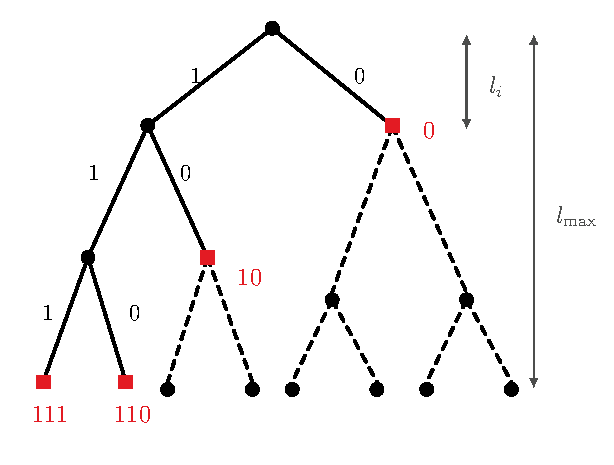
\includegraphics[width=0.5\linewidth]{kraft-mcmillan/kraft-mcmillan_vector.pdf}
    \caption{Rappresentazione albero d-ario Kraft-McMillan.}
    \label{fig:kraft-mcmillan}
\end{figure}

Scegliere un nodo significa 'consumare' una specifica porzione dell'albero. La disuguaglianza di Kraft-McMillan somma queste singole frazioni consumate per verificare che non superino il 100\% dello spazio disponibile. Per esempio, in un albero binario, usare un nodo al primo livello consuma fisicamente metà dell'albero; nella formula, questa scelta pesa esattamente per $2^{-1}$.

Questa lettura rende più intuitiva la selezione dei nodi e il taglio dei discendenti usati nella costruzione di un codice a prefisso.

\begin{proof}[\textbf{Dimostrazione della condizione necessaria}]
    Ipotizziamo che $C$ sia un codice univocamente decodificabile (UD) con $m$ parole di codifica con delle lunghezze rispettive di $\{l_1,l_2,\ldots,l_m\}$ su un alfabeto formato da $d$ simboli. Consideriamo la quantità:
    \[
        \left(\sum_{i=1}^m d^{-l_i}\right)^n = \left(d^{-l_1}+d^{-l_2}+\ldots+d^{-l_m} \right)^n
    \]
    sviluppando questa potenza, otteniamo $m^n$ termini. Ogni termine è il prodotto di un gruppo di $n$ termini per cui ha la forma\footnote{Avendo tutti la stessa base quando viene svolta la potenza tutti i termini vengono raggruppati sotto una sola potenza.} $d^{-l_{i_1}-l_{i_2}-\ldots-l_{i_n}}=d^{-k}$, dove $k$ è la somma delle lunghezze di $n$ parole ($k=l_{i_1}+l_{i_2}+\ldots+l_{i_n}$). Il valore minimo di $k$ è $n$ (se tutte le parole sono lunghe 1) e il massimo è $nL$ (se tutte sono lunghe L). Raggruppiamo tutti i termini che hanno lo stesso esponente $k$ e otteniamo:
    \[
        \sum_{k=n}^{nL} N_k \cdot d^{-k}
    \]
    dove $N_k$ rappresenta il numero di possibili sequenze (concatenazioni di parole) composte da $n$ parole che hanno una lunghezza totale pari a $k$, ovvero il numero di volte che compare il termine $d^{-k}$. Poiché il codice deve essere \textbf{UD per ipotesi}, ogni concatenazione valida di parole deve corrispondere a una stringa univoca di simboli. Il numero massimo di stringhe distinte di lunghezza $k$ creabili con $d$ lettere è $d^k$.\footnote{Si pensi al semplice e familiare caso binario le possibili combinazioni di simboli per $k$ sarebbero proprio $2^k$.}Pertanto, $N_k$ non può mai superare $d^k$ ovvero:
    \[
        N_k\leq d^k
    \]
    applicando il caso limite ($N_k=d^k$) otteniamo:
    \[
        \sum_{k=n}^{nL} d^k \cdot d^{-k} = \sum_{k=n}^{nL} 1 = nL-n+1 \approx nL
    \]
    ricapitolando vale:
    \[
        \left(\sum_{i=1}^m d^{-l_i}\right)^n \leq \sum_{k=n}^{nL} d^k \cdot d^{-k} \leq nL
    \]
    abbiamo quindi dimostrato che esiste un limite superiore pari proprio a $nL$ (questo se tutte le parole nelle combinazioni sono lunghe $L$). Per far sì che la disequazione sia verificata è necessario che la somma sia minore o uguale a $1$. Infatti, ponendo:
    \[
        X = \sum_{i=1}^m d^{-l_i},
    \]
    se per assurdo fosse $X > 1$, allora elevando alla $n$-esima si avrebbe $X^n \to +\infty$ per $n \to +\infty$. D'altra parte, dal lato opposto si ottiene una quantità che cresce al più linearmente in $n$\footnote{La potenza va all'infinito molto più velocemente di una funzione lineare. Si dice che la funzione potenza sia di ordine superiore alla funzione lineare.}. Ne segue che, per $n$ sufficientemente grande, la disuguaglianza non può più essere soddisfatta.

    Si conclude quindi che deve necessariamente valere:
    \[
        \sum_{i=1}^m d^{-l_i} \leq 1.
    \]
\end{proof}

\subsubsection{Proprietà}
Un aspetto rilevante da considerare è distinguere il caso in cui la disequazione sia strettamente minore di $1$ da quello in cui sia esattamente uguale a $1$.

\begin{itemize}
    \item Se la somma è \textbf{strettamente minore di 1}, il codice non è completo: ciò significa che, nella costruzione dell'albero associato al codice, rimangono ancora foglie libere, cioè combinazioni non assegnate ad alcuna parola di codice. In questo caso, quindi, esiste ancora spazio per aggiungere nuove parole senza violare la struttura del codice.

    \item Se la somma è \textbf{esattamente uguale a 1}, il codice è completo: tutte le possibilità compatibili con la struttura del codice sono state sfruttate. Nell'albero non rimangono più foglie utilizzabili per introdurre nuove parole senza compromettere le proprietà del codice stesso.
\end{itemize}

\uline{È importante osservare che questo non significa che ogni sequenza di simboli sia necessariamente una parola valida o una concatenazione decodificabile}. Significa invece che, nel caso di uguaglianza, lo spazio disponibile è stato saturato completamente, mentre nel caso di stretta disuguaglianza rimane ancora spazio inutilizzato.

Consideriamo ora il confronto tra i codici B e C, presenti nel prossimo esercizio. Il codice B è costituito dalle parole:
\[
    0,\quad 100,\quad 110,\quad 111,
\]
mentre il codice C è costituito dalle parole:
\[
    0,\quad 10,\quad 110,\quad 111.
\]

Nel codice B rimane ancora una combinazione disponibile, ad esempio $101$, che non è stata assegnata ad alcun simbolo. Questo mostra che il codice non sfrutta completamente tutte le possibilità offerte dalla sua struttura: infatti, si potrebbe aggiungere la parola $101$ senza distruggere la proprietà di prefisso.

Nel codice C, invece, una situazione del genere non si verifica. La parola $10$ è già presente nel codice e, proprio per questo, tutte le sequenze che iniziano con $10$, come $100$ e $101$, non possono più essere usate come nuove parole di codice. Di conseguenza, il codice C non lascia più spazio per ulteriori assegnazioni ed è quindi completo.

Si noti però che la sequenza $101$ \textbf{non è decodificabile} né nel codice B né nel codice C. Nel codice B ciò accade perché le uniche parole che iniziano con $1$ sono $100$, $110$ e $111$; di conseguenza, né $101$ né una sequenza che inizi con tale prefisso possono essere riconosciute nel loro tratto iniziale come parole valide del codice (proprio per questo è incompleto). Nel codice C, invece, il prefisso $10$ è effettivamente una parola di codice: per questo una sequenza che inizi con $101$ non è immediatamente impossibile, ma richiede la ricezione di ulteriori simboli per verificare se la parte rimanente possa completare una concatenazione valida. La differenza essenziale è quindi che il codice B lascia alcune \uline{combinazioni inutilizzate  senza poterle interpretare}, mentre il codice C \uline{sfrutta in modo più completo la propria struttura}.

\subsubsection{Esempi}
Data la tabella con i seguenti codici:
\begin{table}[htbp]
    \centering
    \begin{tabular}{|c|c|c|c|c|c|}
        \hline
        \textbf{Simbolo} & \textbf{Codice A} & \textbf{Codice B} & \textbf{Codice C} & \textbf{Codice D} & \textbf{Codice E} \\ \hline
        $s_1$            & \lbox{00}         & \lbox{0}          & \lbox{0}          & \lbox{0}          & \lbox{0}          \\ \hline
        $s_2$            & \lbox{01}         & \lbox{100}        & \lbox{10}         & \lbox{100}        & \lbox{10}         \\ \hline
        $s_3$            & \lbox{10}         & \lbox{110}        & \lbox{110}        & \lbox{110}        & \lbox{110}        \\ \hline
        $s_4$            & \lbox{11}         & \lbox{111}        & \lbox{111}        & \lbox{11}         & \lbox{11}         \\ \hline
    \end{tabular}
\end{table}

grazie alla disuguaglianza di Kraft-McMillan possiamo capire quali tra questi potrebbero essere codici istantanei.
\begin{itemize}
    \item Codice A:
          \[
              \sum_{i=1}^4 2^{-2}=\sum_{i=2}^2 4\cdot 2^{-i}=1
          \]
          ho usato entrambe le forme della dimostrazione. La disuguaglianza viene rispettata, si può quindi presumere che il codice A possa essere a prefisso visto che un codice binario con queste lunghezze può essere a prefisso. Per verificarlo bisogna usare l'algoritmo di Sardinas-Patterson (già verificato negli esempi precedenti).
    \item Codice B:
          \[
              \sum_{i=1}^4 2^{-l_i}=2^{-1}+2^{-3}+2^{-3}+2^{-3}=\frac{7}{8}\leq 1
          \]
          queste lunghezze sono valide per un codice a prefisso; da un'analisi più approfondita si può facilmente verificare che questo è un codice a prefisso.
    \item Codice C:
          \[
              \sum_{i=1}^4 2^{-l_i}=2^{-1}+2^{-2}+2^{-3}+2^{-3}=\frac{8}{8}= 1
          \]
          la condizione viene soddisfatta. Questo codice è a prefisso e sfrutta pienamente le possibili combinazioni delle varie lunghezze.
    \item Codice D:
          \[
              \sum_{i=1}^4 2^{-l_i}=2^{-1}+2^{-2}+2^{-3}+2^{-3}=\frac{8}{8}= 1
          \]
          questo codice soddisfa la condizione per essere a prefisso, come il codice C, ma al contrario di suddetto codice non è a prefisso. Infatti, solo per queste lunghezze viene assicurato che ci possa essere un codice a prefisso ma la scelta della concatenazione dei simboli è fondamentale per far si che questo codice sia veramente a prefisso. Si nota subito \textbf{che non è UD } visto che 11 è prefisso di 110 e il residuo è un'altra parola del codice.
    \item Codice E:
          \[
              \sum_{i=1}^4 2^{-l_i}=2^{-1}+2^{-2}+2^{-3}+2^{-2}=1+\frac{1}{8}
          \]
          questo codice non soddisfa la disuguaglianza, possiamo quindi concludere che non è istantaneo.
\end{itemize}
% Fare esercizio direttamente qua per fare capire come si costruisce il codice
\subsubsection{Esercizio guidato}
Si vuole codificare una sorgente con 9 simboli usando un codice a prefisso. L'alfabeto per le parole di codifica è {0,1,2} con delle lunghezze di 1,2,2,2,2,2,3,3,3.

Per prima cosa applichiamo il teorema di Kraft-McMillan per capire se con queste premesse può essere creato un codice a prefisso.
\[
    \sum_{i=1}^9 3^{l_i} = \sum_{k=1}^3 N_k\cdot 3^{-i} = 1\cdot 3^{-1} + 5\cdot 3^{-2} + 3\cdot 3^{-3}=1
\]
la disuguaglianza viene verificata si deduce che con questo alfabeto e queste lunghezze si può costruire un codice a prefisso.

\begin{figure}[htpb]
    \centering
    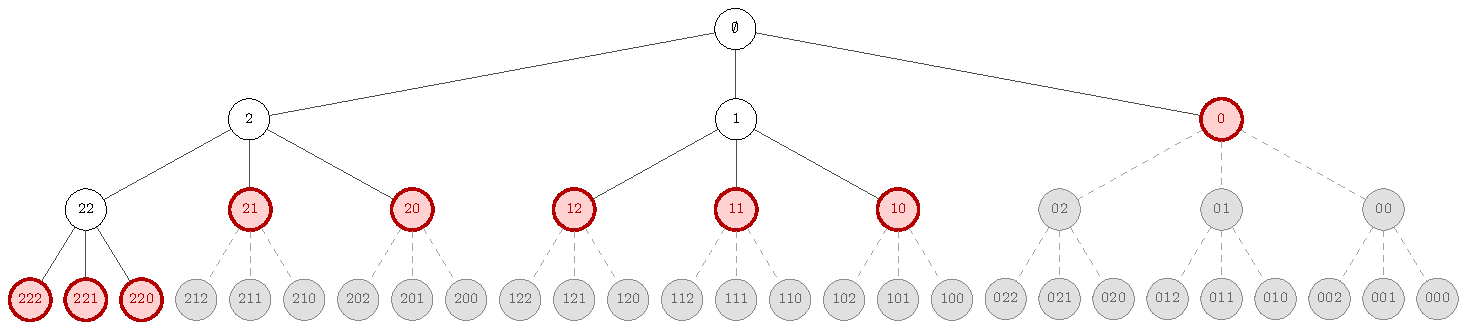
\includegraphics[width=\textwidth]{kraft-mcmillan/albero-ternario}
    \caption{Albero ternario verticale di profondità 3 con una possibile selezione di parole di codice. I nodi scelti sono evidenziati in rosso; i loro discendenti risultano oscurati perché non sono più disponibili.}
    \label{fig:albero-ternario}
\end{figure}

Come si nota in \autoref{fig:albero-ternario} la costruzione del codice a prefisso avviene selezionando i nodi dell'albero ternario in modo da rispettare le lunghezze specificate. Si parte dal livello più basso (lunghezza 1) e viene scelto uno dei nodi di questa lunghezza, ad esempio $0$. Questo nodo diventa una foglia e tutte le sue diramazioni (i suoi discendenti) vengono oscurati perché non possono più essere usati. Si passa poi al livello successivo (lunghezza 2) e si scelgono 5 nodi, ad esempio $10$, $11$, $12$, $20$ e $21$. Anche questi diventano foglie e i loro discendenti vengono oscurati. Infine, si passa all'ultimo livello (lunghezza 3) e si scelgono i 3 nodi rimanenti, ad esempio $220$, $221$ e $222$. In questo modo, si garantisce che il codice risultante sia a prefisso e quindi istantaneo. Una possibile assegnazione dei simboli è:
\begin{table}[htbp]
    \centering
    \begin{tabular}{|c|c|}
        \hline
        \textbf{Simbolo} & \textbf{Codice} \\ \hline
        $s_1$            & \lbox{0}        \\ \hline
        $s_2$            & \lbox{10}       \\ \hline
        $s_3$            & \lbox{11}       \\ \hline
        $s_4$            & \lbox{12}       \\ \hline
        $s_5$            & \lbox{20}       \\ \hline
        $s_6$            & \lbox{21}       \\ \hline
        $s_7$            & \lbox{220}      \\ \hline
        $s_8$            & \lbox{221}      \\ \hline
        $s_9$            & \lbox{222}      \\ \hline
    \end{tabular}
\end{table}

\subsection{Lunghezza media dei codici}
Per decidere quale sia il codice più adatto a rappresentare una certa sorgente è necessario calcolare la lunghezza media dei codici per capire quale sia il più efficiente.
\begin{definizione}
    Dato un codice $C$ con un alfabeto di sorgente $S=\{s_1,s_2,\ldots,s_m\}$ e un alfabeto di codifica $X=\{x_1,x_2,\ldots,x_d\}$. Siano $\{c_1,c_2,\ldots,c_m\}$ le parole di codifica con delle lunghezze rispettive $\{l_1,l_2,\ldots,l_m\}$ e siano $\{p_1,p_2,\ldots,p_m\}$ le probabilità dei simboli di sorgente. La lunghezza media del codice $C$ è definita come:
    \[
        L_S(C) = \sum_{i=1}^m p_i \cdot l_i
    \]
\end{definizione}
Il miglior codice che possa essere scelto per rappresentare una sorgente è quello che minimizza la lunghezza media.

\subsubsection{Limite inferiore della lunghezza media}
Il Teorema di Shannon stabilisce il limite matematico inferiore per la lunghezza media di un codice univocamente decodificabile (UD).
\begin{theorem}
    Se $C$ è un codice unicamente decodificabile (UD) per una sorgente $S$ con probabilità $p_1,p_2,\ldots,p_m$ e alfabeto di codifica $X$ caratterizzato da $d$ simboli differenti, allora vale:
    \begin{equation}
        L_S(C) \geq \frac{H(S)}{\log d}
    \end{equation}
    dove $H(S)$ è l'entropia della sorgente $S$ e $\log d$ rappresenta il numero di bit necessari per codificare ogni simbolo dell'alfabeto di codifica $X$. Per codici binari si può dedurre che il limite inferiore è proprio l'entropia della sorgente, ovvero:
    \[
        L_S(C) \geq H(S).
    \]
\end{theorem}
\begin{proof}
    Dalla disuguaglianza di Kraft-McMillan \eqref{eq:disequality_kraft_mcmillan} segue che, se $C$ è un codice univocamente decodificabile (UD), allora:
    \[
        \sum_{i=1}^m d^{-l_i} \leq 1,
    \]
    il che impone un vincolo sulle lunghezze $l_i$ delle parole di codice ammissibili.

    Per mettere in relazione tale vincolo con le probabilità della sorgente, introduciamo $m$ numeri non negativi $q_i$ (che rappresenta la distribuzione $\{q_i\}_{i=1}^m$) tali che $\sum_{i=1}^m q_i = 1$. Vale allora la seguente disuguaglianza\footnote{In questo modo si costruisce un collegamento diretto tra le probabilità della sorgente $(p_i)$, che determinano l’entropia, e una distribuzione $(q_i)$ che, nel contesto della codifica, rappresenta implicitamente le lunghezze del codice.}:
    \begin{equation}\label{eq:teorema_shannon_dimostrazione_passaggio_3}
        \sum_{i=1}^m p_i \log\!\left(\frac{1}{p_i}\right)
        \;\leq\;
        \sum_{i=1}^m p_i \log\!\left(\frac{1}{q_i}\right),
    \end{equation}

    con uguaglianza se e solo se $q_i = p_i$ per ogni $i$. La quantità a destra rappresenta la \textbf{media}, rispetto alla distribuzione vera $p$, del costo logaritmico $\log\!\left(\frac{1}{q_i}\right)$ associato ai simboli $s_i$\footnote{In altre parole, ad ogni simbolo $s_i$ è associato un costo rappresentato da $\log\!\left(\frac{1}{q_i}\right)$; la disuguaglianza afferma che la media di questi costi, calcolata con le probabilità reali $p_i$, è sempre maggiore o uguale all'entropia della sorgente.
        Scegliendo pesi che si discostano dalle probabilità reali $p_i$, si introduce un costo aggiuntivo che rende la media maggiore perchè non si riesce a rispecchiare la frequenza reale dei simboli.}.

    Questa relazione costituisce il passaggio chiave per derivare un limite inferiore alla lunghezza media dei codici. Per verificarla, considero la differenza tra i due membri e la riscrivo nella forma:
    \begin{align*}
        \sum_{i=1}^m p_i \log\!\left(\frac{1}{p_i}\right)
        - \sum_{i=1}^m p_i \log\!\left(\frac{1}{q_i}\right)
         & = \sum_{i=1}^m p_i \log\!\left(\frac{q_i}{p_i}\right)
    \end{align*}
    cambiando la base del logaritmo ottengo:
    \begin{align*}
        \sum_{i=1}^m p_i \log\!\left(\frac{q_i}{p_i}\right)
         & = \sum_{i=1}^m p_i\;\frac{\ln\left(\frac{q_i}{p_i}\right)}{\ln 2}   \\
         & = \frac{1}{\ln 2}\sum_{i=1}^m p_i \ln\!\left(\frac{q_i}{p_i}\right)
    \end{align*}
    A questo punto, usando la proprietà\footnote{Per capire questa proprietà basta tracciare i grafici delle due funzioni.} $\ln x \leq x-1$, segue che:
    \begin{align*}
        \sum_{i=1}^m p_i \log\!\left(\frac{q_i}{p_i}\right)
         & \leq \frac{1}{\ln 2}\sum_{i=1}^m p_i \!\left(\frac{q_i}{p_i} - 1\right) \\
         & = \frac{1}{\ln 2}\sum_{i=1}^m (q_i - p_i)                               \\
         & = \frac{1}{\ln 2}\left(\sum_{i=1}^m q_i - \sum_{i=1}^m p_i\right) = 0
    \end{align*}
    Quindi:
    \[
        \sum_{i=1}^m p_i \log\!\left(\frac{q_i}{p_i}\right) \leq 0,
    \]
    visto che entrambe sono distribuzioni le cui somme sono uguali a 1. In questi passaggi abbiamo dimostrato la disuguaglianza chiave che \uline{mette in relazione l'entropia della sorgente con una media logaritmica basata su una distribuzione arbitraria} $q_i$.

    Scegliamo:
    \[
        q_i=\frac{d^{-l_i}}{\sum_{j=1}^m d^{-l_j}}.
    \]
    Questa scelta è naturale: i valori $q_i$ vengono costruiti a partire dai termini $d^{-l_i}$ che compaiono nella disuguaglianza di Kraft-McMillan dipendendo direttamente dalle lunghezze $l_i$ delle codeword; si può quindi collegare il risultato del punto precedente proprio alla lunghezza del codice.\footnote{La normalizzazione al denominatore serve a fare in modo che i valori $q_i$ sommino a $1$, così da ottenere una distribuzione di probabilità e poter applicare il risultato precedente.}.

    Sostituendo nella formula \eqref{eq:teorema_shannon_dimostrazione_passaggio_3} otteniamo:
    \begin{align*}
        H(S)  = \sum_{i=1}^m p_i \log\!\left(\frac{1}{p_i}\right)
         & \leq \sum_{i=1}^m p_i \log\!\left(\frac{1}{q_i}\right)
        = \sum_{i=1}^m p_i \log\!\left(\frac{\sum_{j=1}^m d^{-l_j}}{d^{-l_i}}\right)                 \\
         & = \sum_{i=1}^m p_i \left[\log\!\left(\sum_{j=1}^m d^{-l_j}\right) - \log d^{-l_i}\right]  \\
         & = \sum_{i=1}^m p_i \log\!\left(\sum_{j=1}^m d^{-l_j}\right) + \sum_{i=1}^m p_i l_i \log d \\
         & = \log\!\left(\sum_{j=1}^m d^{-l_j}\right) + L_S(C)\cdot \log d
    \end{align*}
    visto che $C$ è per ipotesi un codice UD allora $\sum_{j=1}^m d^{-l_j} \leq 1$, segue che:
    \begin{align*}
        \log\!\left(\sum_{j=1}^m d^{-l_j}\right) + L_S(C)\cdot \log d
         & \leq L_S(C)\cdot \log d
    \end{align*}
    allora si conclude che:
    \[
        H(S) \leq L_S(C)\cdot \log d
        \quad\Rightarrow\quad
        L_S(C) \geq \frac{H(S)}{\log d}.
    \]
\end{proof}
Ricapitolando, la dimostrazione si basa su questi punti:
\begin{enumerate}
    \item \textbf{Punto di partenza:} Si utilizza la disuguaglianza di Kraft-McMillan per i codici univocamente decodificabili (UD).
    \item \textbf{Variabili ausiliarie:} Si introduce un set di numeri arbitrari ($q_i$) la cui somma è pari a 1.
    \item \textbf{Disuguaglianza logaritmica:} Si applica una proprietà matematica dei logaritmi per mettere in relazione le probabilità della sorgente ($p_i$) con i numeri $q_i$.
    \item \textbf{Sostituzione strategica:} Si assegna ai numeri $q_i$ un valore specifico basato sulle lunghezze delle parole di codifica.
    \item \textbf{Conclusione:} Si combinano i risultati per dimostrare che l'entropia è sempre minore o uguale alla lunghezza media.
\end{enumerate}

\subsubsection{Efficienza e ridondanza}
Per misurare l'efficienza di un codice $C$ si può usare la seguente formula:
\[
    \theta(C) = \frac{H_d(S)}{L_S(C)} = \frac{H(S)}{L_S(C)\cdot \log d}
\]
dove $0 \leq \theta(C) \leq 1$. Più il valore tende a 1 e più il codice è efficiente, mentre più si discosta da 1 e meno è efficiente. Se $C$ è un codice compatto allora $\theta(C)=1$.

Per misurare la ridondanza di un codice $C$ (quanto un codice si discosta dall'ottimalità) si può invece usare la seguente formula:
\[
    \rho(C) = 1- \theta(C) = \frac{L_S(C) - H_d(S)}{L_S(C)}
\]
dove $0 \leq \rho(C) \leq 1$. Più il valore tende a 1 e più il codice è ridondante, mentre più si discosta da 1 e meno ridondante risulta. Se $C$ è un codice compatto allora $\rho(C)=0$. La ridondanza rappresenta la porzione di lunghezza media che non è strettamente necessaria per rappresentare l'informazione della sorgente, ma che è invece dovuta a inefficienze nella progettazione del codice. Un codice con alta ridondanza utilizza più simboli di codifica del necessario, mentre un codice con bassa ridondanza si avvicina al limite inferiore stabilito dall'entropia della sorgente.

\subsection{Codici ottimali e compatti}
C'è una distinzione netta tra codici ottimali e codici compatti.
\begin{itemize}
    \item Un codice $C$ è detto \textbf{ottimale} se la sua lunghezza media $L_S(C)$ è minimizzata rispetto a tutti i codici UD ammessi per la stessa sorgente $S$. In altre parole, $C$ è ottimale se non esiste alcun altro codice UD che possa rappresentare la sorgente con una lunghezza media inferiore a quella di $C$.
    \item Un codice $C$ è detto \textbf{compatto} se la sua lunghezza media eguaglia l'entropia, ovvero:
          \[
              L_S(C) = H_d(S) = \frac{H(S)}{\log d}
          \]
          Essendo l'entropia il limite inferiore per la lunghezza media, raggiungerlo significa che non esiste alcun altro codice che possa rappresentare la sorgente con una lunghezza media più bassa. Quindi un codice compatto è anche ottimale, ma non vale il viceversa.
\end{itemize}
\paragraph{Nota:}
In un codice a prefisso ottimale, i \textbf{simboli più frequenti} tendono a essere associati a \textbf{parole di codice più corte}, mentre i \textbf{simboli meno frequenti} a \textbf{parole più lunghe}. Questa idea guida la costruzione di codici ottimali come il codice di Huffman.

Se invece la lunghezza media di un codice è \uline{superiore all'entropia}, allora il codice presenta un \textbf{margine di inefficienza}.

\subsubsection{Condizioni di esistenza dei codici compatti}\label{condizioni_codici_compatti}
Dopo aver distinto i codici ottimali dai codici compatti, sorge una domanda naturale: quando è possibile raggiungere esattamente il limite inferiore fornito dal teorema di Shannon? Il caso di uguaglianza caratterizza proprio le situazioni in cui un codice compatto può esistere.

Per un codice univocamente decodificabile (UD) d-ario, l'uguaglianza:
\[
    L_S(C)=H_d(S)
\]
si verifica se e solo se la disuguaglianza di Kraft-McMillan è soddisfatta con uguaglianza, ciò accade quando:
\[
    \left\{
    \begin{aligned}
        p_i & = d^{-l_i},                           \\
        l_i & = \log_d\!\left(\frac{1}{p_i}\right),
    \end{aligned}
    \right.
    \qquad i=1,\ldots,m.
\]
Questo è possibile \uline{solo se} le lunghezze delle parole di codice sono \textbf{numeri interi}\footnote{\`E ovvio che le lunghezze delle parole siano numeri interi, queste infatti misurano quanto ogni parola di codifica debba essere lunga. Quindi se questi valori sono numeri interi allora deve valere che anche il logaritmo sia un numero intero.}, ovvero se $l_i=\log_d\!\left(\frac{1}{p_i}\right)\in \mathbb{N}$ per ogni $i$.

Si nota che scegliendo:
\[
    p_i = \left(\frac{1}{d}\right)^{\alpha_i} = d^{-\alpha_i},
    \qquad \alpha_i \in \mathbb{N},\ \alpha_i > 0
\]
basta scegliere $l_i=\alpha_i$ per ogni $i$ per ottenere un codice compatto. Infatti, con questa scelta possiamo notare che:
\[
    \sum_{i=1}^m d^{-l_i} = \sum_{i=1}^m d^{-\alpha_i} = \sum_{i=1}^m p_i = 1
\]

\subsubsection{Esempio}
Dato la seguente sorgente con 4 simboli:
\begin{table}[htpb]
    \centering
    \begin{tabular}{|l|l|l|l|}
        \hline
        \textbf{Simbolo} & \textbf{Probabilità} & \textbf{Codice 1} & \textbf{Codice 2} \\ \hline
        $s_1$            & 0.5                  & 0                 & 0                 \\ \hline
        $s_2$            & 0.25                 & 10                & 10                \\ \hline
        $s_3$            & 0.125                & 110               & 110               \\ \hline
        $s_4$            & 0.125                & 111               & 1110              \\ \hline
    \end{tabular}
\end{table}

quale dei due codici è un codice compatto?

Per verificare se un codice è compatto, bisogna calcolare la lunghezza media di ciascun codice e confrontarla con l'entropia della sorgente. L'entropia della sorgente $S$ è calcolata come segue:
\[
    H(S) = \sum_{i=1}^4 p_i \log_2 \frac{1}{p_i} = \frac{1}{2}\log_2 2 + \frac{1}{4}\log_2 4 + \frac{1}{8}\log_2 8 + \frac{1}{8}\log_2 8 = 1.75 \text{ bit/symbol}.
\]
Calcoliamo ora la lunghezza media per ciascun codice:
\begin{itemize}
    \item \textbf{Codice 1:}
          \[
              L_S(C_1) = \sum_{i=1}^4 p_i \cdot l_i = 0.5\cdot 1 + 0.25\cdot 2 + 0.125\cdot 3 + 0.125\cdot 3 = 1.75 = H(S)
          \]
          La lunghezza media del Codice 1 è esattamente uguale all'entropia della sorgente, quindi il Codice 1 è un codice compatto.
    \item \textbf{Codice 2:}
          \[
              L_S(C_2) = \sum_{i=1}^4 p_i \cdot l_i = 0.5\cdot 1 + 0.25\cdot 2 + 0.125\cdot 3 + 0.125\cdot 4 = 1.875 > H(S)
          \]
          La lunghezza media del Codice 2 è superiore all'entropia della sorgente, quindi il Codice 2 non è un codice compatto.
\end{itemize}
\newpage
\subsubsection{Esercizio}
Data la seguente sorgente:
\begin{table}[htpb]
    \centering
    \begin{tabular}{|l|l|}
        \hline
        \textbf{Simbolo} & \textbf{Probabilità} \\ \hline
        $s_0$            & 1/3                  \\ \hline
        $s_1$            & 1/3                  \\ \hline
        $s_2$            & 1/9                  \\ \hline
        $s_3$            & 1/9                  \\ \hline
        $s_4$            & 1/27                 \\ \hline
        $s_5$            & 1/27                 \\ \hline
        $s_6$            & 1/27                 \\ \hline
    \end{tabular}
\end{table}

trovare un codice compatto per l'alfabeto di codifica $\{0,1,2\}$.
Il primo passo da fare è calcolare l'entropia della sorgente:
\begin{align*}
    H(S)
     & = \sum_{i=0}^6 p_i \log_3 \frac{1}{p_i}   \\
     & = 2 \cdot \frac{1}{3}\log_3 3
    + 2 \cdot \frac{1}{9}\log_3 9
    + 3 \cdot \frac{1}{27}\log_3 27              \\
     & = 2 \cdot \frac{1}{3}\cdot 1
    + 2 \cdot \frac{1}{9}\cdot 2
    + 3 \cdot \frac{1}{27}\cdot 3                \\
     & = \frac{2}{3} + \frac{4}{9} + \frac{1}{3} \\
     & = \frac{13}{9}
\end{align*}
Per costruire un codice compatto so che devo assegnare a ciascun simbolo una parola di codice la cui lunghezza sia pari a $l_i = \log_3\!\left(\frac{1}{p_i}\right)$. Calcoliamo quindi le lunghezze per ciascun simbolo:
\begin{align*}
    l_0 = l_1       & = \log_3 3 = 1,  \\
    l_2 = l_3       & = \log_3 9 = 2,  \\
    l_4 = l_5 = l_6 & = \log_3 27 = 3.
\end{align*}
Ricapitolando, le lunghezze delle parole di codice devono essere $\{1,1,2,2,3,3,3\}$ con le quali è possibile costruire un codice a prefisso, ad esempio:
\begin{table}[htpb]
    \centering
    \begin{tabular}{|l|l|}
        \hline
        \textbf{Simbolo} & \textbf{Codice} \\ \hline
        $s_0$            & 0               \\ \hline
        $s_1$            & 1               \\ \hline
        $s_2$            & 20              \\ \hline
        $s_3$            & 21              \\ \hline
        $s_4$            & 220             \\ \hline
        $s_5$            & 221             \\ \hline
        $s_6$            & 222             \\ \hline
    \end{tabular}
\end{table}

verificando che la lunghezza media di questo codice è:
\[
    L_S(C) = \sum_{i=0}^6 p_i \cdot l_i
    = 2 \cdot \left(\frac{1}{3}\cdot 1\right)
    + 2 \cdot \left(\frac{1}{9}\cdot 2\right)
    + 3 \cdot \left(\frac{1}{27}\cdot 3\right)
    = \frac{13}{9} = H(S)
\]
allora si conclude che il codice costruito è compatto.

\section{Algoritmi di codifica}
Nel seguente capitolo verranno affrontati le teorie e i relativi algoritmi per costruire codici a prefisso e ottimali.

\subsection{Codifica Shannon}
Nelle condizioni di esistenza viste nel paragrafo \eqref{condizioni_codici_compatti} abbiamo visto che, per ottenere un codice compatto, le lunghezze ideali devono soddisfare:
\[
    l_i = \log_d\!\left(\frac{1}{p_i}\right).
\]
Tuttavia tali valori non sono in generale interi, mentre le lunghezze delle parole di codice devono necessariamente esserlo.

La codifica di Shannon nasce proprio per superare questa difficoltà. Essa sostituisce alle lunghezze ideali delle lunghezze intere, ottenendo così un codice a prefisso effettivamente costruibile e con lunghezza media vicina al limite inferiore teorico.

\begin{theorem}\label{teorema_shannon_limite_sup_inf}
    Sia $S$ una sorgente con simboli $s_1, s_2, \ldots, s_m$ e probabilità associate $p_1, p_2, \ldots, p_m$, e sia $X$ un alfabeto di codifica d-ario. Se per ogni $i=1,\ldots,m$ si sceglie:
    \[
        l_i = \left\lceil \log_d\!\left(\frac{1}{p_i}\right) \right\rceil,
    \]
    allora esiste un codice a prefisso $C$ le cui parole di codice hanno lunghezza $l_i$ e la cui lunghezza media soddisfa:
    \[
        H_d(S) \leq L_S(C) < H_d(S) + 1.
    \]
\end{theorem}
\begin{proof}
    Per definizione di arrotondamento all'intero superiore, per ogni $i$ vale\footnote{Se poniamo $x=\log_d\!\left(\frac{1}{p_i}\right)$ e scegliamo $l_i=\lceil x \rceil$, allora $l_i$ è il più piccolo intero maggiore o uguale a $x$. Quindi deve valere $x \leq l_i < x+1$.}:
    \[
        \log_d\!\left(\frac{1}{p_i}\right) \leq l_i < \log_d\!\left(\frac{1}{p_i}\right)+1
    \]
    Dalla prima disuguaglianza, elevando a potenza con base $d$, otteniamo:
    \[
        d^{-l_i} \leq p_i
    \]
    Sommando su tutti gli $i$, segue che:
    \[
        \sum_{i=1}^m d^{-l_i} \leq \sum_{i=1}^m p_i = 1
    \]
    quindi, per la disuguaglianza di Kraft-McMillan, esiste un codice a prefisso $C$ con le lunghezze specificate.

    Moltiplicando ora la doppia disuguaglianza iniziale per $p_i$ e sommando su tutti gli $i$, otteniamo:
    \[
        \sum_{i=1}^m p_i \log_d\!\left(\frac{1}{p_i}\right)
        \leq
        \sum_{i=1}^m p_i l_i
        <
        \sum_{i=1}^m p_i \log_d\!\left(\frac{1}{p_i}\right) + \sum_{i=1}^m p_i
    \]
    Poiché
    \[
        H_d(S)=\sum_{i=1}^m p_i \log_d\!\left(\frac{1}{p_i}\right),
        \qquad
        L_S(C)=\sum_{i=1}^m p_i l_i,
        \qquad
        \sum_{i=1}^m p_i = 1,
    \]
    concludiamo che:
    \[
        H_d(S) \leq L_S(C) < H_d(S) + 1.
    \]
\end{proof}
\paragraph{Nota:}
La codifica di Shannon non produce in generale un codice compatto, ma garantisce che la lunghezza media del codice \uline{si discosti dall'entropia per meno di un simbolo di codifica}. Facendo riferimento al caso binario, l'eccesso rispetto all'entropia è quindi strettamente minore di $1$ bit per simbolo.

\subsubsection{Costruzione a sorgente singola}
Per costruire concretamente un codice secondo la codifica di Shannon bisogna distinguere due passaggi. Il primo passaggio consiste nel fissare le lunghezze:
\[
    l_i = \left\lceil \log_d\!\left(\frac{1}{p_i}\right) \right\rceil.
\]
Il secondo passaggio consiste nell'assegnare parole di codice effettive che abbiano proprio quelle lunghezze. Le lunghezze, infatti, indicano soltanto a quale livello dell'albero d-ario devono trovarsi le foglie, ma non determinano in modo unico quale parola di codice assegnare a ciascun simbolo.

In particolare:
\begin{enumerate}
    \item si ordinano i simboli in ordine di probabilità decrescente;
    \item si calcola per ciascun simbolo la lunghezza $l_i$;
    \item si scelgono nell'albero d-ario delle foglie poste ai livelli $l_i$, evitando che una parola scelta sia prefisso di un'altra;
    \item si associano ai simboli le parole di codice ottenute.
\end{enumerate}

La disuguaglianza di Kraft-McMillan assicura che una tale costruzione è possibile. In questo modo i simboli più probabili ricevono parole più corte, mentre quelli meno probabili ricevono parole più lunghe.

\paragraph{Nota sulle probabilità cumulative:}
Un modo canonico per scegliere le parole di codice, una volta fissate le lunghezze, usa le \textbf{probabilità cumulative}:
\[
    Q_i = \sum_{j=1}^{i-1} p_j.
\]
La probabilità cumulativa non serve a calcolare $l_i$, né modifica la lunghezza media del codice: serve solo a ricavare in modo sistematico una possibile parola di codice. Nel caso binario si prende lo sviluppo binario di $Q_i$ e si conservano le prime $l_i$ cifre dopo la virgola.

Ad esempio, per una sorgente con probabilità $\frac{1}{2}, \frac{1}{4}, \frac{1}{8}, \frac{1}{8}$ si ottengono le lunghezze $1,2,3,3$ e:
\begin{center}
    \begin{tabular}{|l|l|l|l|l|}
        \hline
        \textbf{Simbolo} & \textbf{$Q_i$} & \textbf{$Q_i$ in base 2} & \textbf{$l_i$} & \textbf{Codice} \\ \hline
        $s_1$            & $0$            & $0.000\ldots_2$          & $1$            & \lbox{0}        \\ \hline
        $s_2$            & $1/2$          & $0.100\ldots_2$          & $2$            & \lbox{10}       \\ \hline
        $s_3$            & $3/4$          & $0.110\ldots_2$          & $3$            & \lbox{110}      \\ \hline
        $s_4$            & $7/8$          & $0.111\ldots_2$          & $3$            & \lbox{111}      \\ \hline
    \end{tabular}
\end{center}
Quindi la cumulativa è solo un criterio ordinato per scegliere le parole di codice; se l'esercizio richiede soltanto lunghezza media, efficienza e ridondanza, non è necessario usarla.

Questa costruzione non va confusa con la codifica Shannon-Fano: qui le lunghezze sono già decise dalla formula logaritmica; in Shannon-Fano, invece, l'albero viene costruito dividendo ricorsivamente i simboli in gruppi di probabilità simile.

\subsubsection{Codifica di Shannon a blocchi}
La codifica di Shannon a sorgente singola non garantisce in generale di ottenere un codice compatto o ottimale. Per ridurre lo scarto medio rispetto all'entropia si può applicare la stessa idea non ai singoli simboli, ma a blocchi di simboli. Questa è un'estensione teorica della codifica di Shannon, non la codifica Shannon-Fano.

Si considera quindi la sorgente estesa $S^n$, i cui simboli sono tutte le n-uple di simboli della sorgente originaria (essa rappresenta l'insieme di tutti i possibili blocchi di lunghezza $n$) e la probabilità di ciascun blocco è il prodotto delle probabilità dei simboli che lo compongono.

\begin{theorem}
    Data una sorgente $S$ vale la seguente:
    \[
        H_d(S^n) = n \cdot H_d(S)
    \]
    ovvero, l'entropia della sorgente estesa $S^n$ è pari a $n$ volte l'entropia della sorgente originaria $S$.
\end{theorem}

Si definisce quindi come lunghezza media per simbolo di un codice $C$ per la sorgente estesa $S^n$ la quantità:
\[
    L_n(C) := \frac{L_{S^n}(C)}{n}
\]

\paragraph{Interpretazione}
Considerando la sorgente estesa:
\[
    S^n = \{(s_{i_1}, s_{i_2},\ldots, s_{i_n}) : s_{i_k} \in S\},
\]
la probabilità, come già detto, di ciascun blocco di simboli è:
\[
    P(s_{i_1}, s_{i_2},\ldots, s_{i_n}) = p_{i_1} \cdot p_{i_2} \cdot \ldots \cdot p_{i_n}
\]
essenzialmente, ogni blocco viene trattato come un simbolo unico con una probabilità che è il prodotto delle probabilità dei simboli che lo compongono. Allora considerando il \autoref{teorema_shannon_limite_sup_inf} per la sorgente estesa $S^n$ vale:
\[
    H_d(S^n) \leq L_{S^n}(C) < H_d(S^n) + 1
\]
dividendo per $n$ otteniamo:
\[
    \frac{H_d(S^n)}{n}  \leq \frac{L_{S^n}(C)}{n}  < \frac{H_d(S^n) + 1}{n}
\]
semplificando:
\[
    H_d(S) \leq L_n(C) < H_d(S) + \frac{1}{n}.
\]
Prendendo blocchi di lunghezza sempre maggiore, ovvero facendo tendere $n$ all'infinito, si ottiene proprio l'entropia della sorgente, cioè:
\[
    \lim_{n\to\infty} L_n(C) = H_d(S).
\]
Il termine $\frac{1}{n}$ rappresenta quindi un limite superiore dell'eccesso della lunghezza media per simbolo rispetto all'entropia: al crescere di $n$ esso tende a zero. Per ogni valore finito di $n$, però, la codifica di Shannon non garantisce in generale di ottenere un codice compatto o ottimale, ma assicura che la lunghezza media per simbolo possa avvicinarsi arbitrariamente all'entropia della sorgente.

Va però osservato che il numero di simboli della sorgente estesa cresce rapidamente con $n$: se la sorgente originaria ha $m$ simboli, allora $S^n$ contiene $m^n$ blocchi distinti. Per questo motivo, sebbene la codifica a blocchi abbia un grande valore teorico, essa diventa presto difficile da gestire in pratica.

\subsubsection{Esempi}
Vediamo ora due esempi in cui la codifica di Shannon non produce un codice compatto.

\paragraph{Sorgente con tre simboli}
Consideriamo la seguente sorgente con alfabeto binario:
\begin{table}[htpb]
    \centering
    \begin{tabular}{|l|l|}
        \hline
        \textbf{Simbolo} & \textbf{Probabilità} \\ \hline
        $s_0$            & 2/3                  \\ \hline
        $s_1$            & 2/9                  \\ \hline
        $s_2$            & 1/9                  \\ \hline
    \end{tabular}
\end{table}

calcoliamo le lunghezze:
\begin{align*}
    l_0 & = \left\lceil \log_2\!\left(\frac{1}{2/3}\right) \right\rceil = \left\lceil 0.58 \right\rceil = 1, \\
    l_1 & = \left\lceil \log_2\!\left(\frac{1}{2/9}\right) \right\rceil = \left\lceil 2.17 \right\rceil = 3, \\
    l_2 & = \left\lceil \log_2\!\left(\frac{1}{1/9}\right) \right\rceil = \left\lceil 3.17 \right\rceil = 4.
\end{align*}
Un possibile codice a prefisso con tali lunghezze è il seguente:
\begin{table}[htpb]
    \centering
    \begin{tabular}{|l|l|}
        \hline
        \textbf{Simbolo} & \textbf{Codice C} \\ \hline
        $s_0$            & \lbox{0}          \\ \hline
        $s_1$            & \lbox{100}        \\ \hline
        $s_2$            & \lbox{1010}       \\ \hline
    \end{tabular}
\end{table}

La lunghezza media di questo codice è:
\begin{align*}
    L_S(C) & = \sum_{i=0}^2 p_i \cdot l_i = \frac{2}{3}\cdot 1 + \frac{2}{9}\cdot 3 + \frac{1}{9}\cdot 4 = \frac{16}{9} \approx 1.78
\end{align*}
mentre l'entropia della sorgente è:
\begin{align*}
    H(S) & = \sum_{i=0}^2 p_i \log_2 \frac{1}{p_i} = \frac{2}{3}\log_2 \frac{3}{2} + \frac{2}{9}\log_2 \frac{9}{2} + \frac{1}{9}\log_2 9 \approx 1.22
\end{align*}
Quindi questo codice ottenuto con la codifica di Shannon \textbf{non è un codice compatto né ottimale}. Infatti è possibile costruire un altro codice a prefisso con lunghezza media più vicina all'entropia, ad esempio:
\begin{table}[htpb]
    \centering
    \begin{tabular}{|l|l|}
        \hline
        \textbf{Simbolo} & \textbf{Codice C'} \\ \hline
        $s_0$            & \lbox{0}           \\ \hline
        $s_1$            & \lbox{10}          \\ \hline
        $s_2$            & \lbox{11}          \\ \hline
    \end{tabular}
\end{table}

con lunghezza media:
\begin{align*}
    L_S(C') & = \frac{2}{3}\cdot 1 + \frac{2}{9}\cdot 2 + \frac{1}{9}\cdot 2 = \frac{4}{3} \approx 1.33
\end{align*}

\paragraph{Sorgente con due simboli}
Consideriamo ora la seguente sorgente con alfabeto binario:
\begin{center}
    \begin{tabular}{|l|l|}
        \hline
        \textbf{Simbolo} & \textbf{Probabilità} \\ \hline
        $s_0$            & 1/4                  \\ \hline
        $s_1$            & 3/4                  \\ \hline
    \end{tabular}
\end{center}

Applicando la codifica di Shannon si ottengono le lunghezze:
\begin{align*}
    l_0 & = \left\lceil \log_2\!\left(\frac{1}{1/4}\right) \right\rceil = \left\lceil 2 \right\rceil = 2,    \\
    l_1 & = \left\lceil \log_2\!\left(\frac{1}{3/4}\right) \right\rceil = \left\lceil 0.41 \right\rceil = 1.
\end{align*}

Un possibile codice a prefisso con tali lunghezze è:
\begin{table}[htpb]
    \centering
    \begin{tabular}{|l|l|}
        \hline
        \textbf{Simbolo} & \textbf{Codice C} \\ \hline
        $s_0$            & \lbox{10}         \\ \hline
        $s_1$            & \lbox{0}          \\ \hline
    \end{tabular}
\end{table}

La lunghezza media del codice è:
\begin{align*}
    L_S(C) & = \frac{1}{4}\cdot 2 + \frac{3}{4}\cdot 1 = \frac{5}{4} = 1.25
\end{align*}
mentre l'entropia della sorgente è:
\begin{align*}
    H(S) & = \frac{1}{4}\log_2 4 + \frac{3}{4}\log_2 \frac{4}{3} \approx 0.81
\end{align*}
quindi il codice ottenuto con la codifica di Shannon non è compatto (ma neanche ottimale).

Inoltre, in questo caso, esso non è nemmeno ottimale. Infatti possiamo considerare il codice:
\begin{table}[htpb]
    \centering
    \begin{tabular}{|l|l|}
        \hline
        \textbf{Simbolo} & \textbf{Codice C'} \\ \hline
        $s_0$            & \lbox{1}           \\ \hline
        $s_1$            & \lbox{0}           \\ \hline
    \end{tabular}
\end{table}

la cui lunghezza media è:
\begin{align*}
    L_S(C') & = \frac{1}{4}\cdot 1 + \frac{3}{4}\cdot 1 = 1.
\end{align*}
Il codice $C'$ è quindi ottimale. Esso non è compatto, perché la sua lunghezza media è ancora maggiore dell'entropia della sorgente, ma in questo caso non è possibile ottenere un codice binario a prefisso con lunghezza media inferiore a $1$.

\subsubsection{Esercizio sulla codifica di Shannon}\label{esercizio_codifica_shannon}
Data la seguente sorgente con alfabeto binario:
\begin{center}
    \begin{tabular}{|l|l|}
        \hline
        \textbf{Simbolo} & \textbf{Probabilità} \\ \hline
        $x_1$            & 0.09                 \\ \hline
        $x_2$            & 0.21                 \\ \hline
        $x_3$            & 0.05                 \\ \hline
        $x_4$            & 0.10                 \\ \hline
        $x_5$            & 0.36                 \\ \hline
        $x_6$            & 0.14                 \\ \hline
        $x_7$            & 0.05                 \\ \hline
    \end{tabular}
\end{center}
trovare la codifica secondo Shannon e calcolare efficienza e ridondanza. Nella codifica di Shannon le lunghezze sono calcolate con:
\[
    l_i = \left\lceil \log_2\!\left(\frac{1}{p_i}\right) \right\rceil.
\]
Otteniamo quindi:
\begin{align*}
    l_1 & = \left\lceil \log_2\left(\frac{1}{0.09}\right) \right\rceil = \left\lceil 3.47 \right\rceil = 4, \\
    l_2 & = \left\lceil \log_2\left(\frac{1}{0.21}\right) \right\rceil = \left\lceil 2.25 \right\rceil = 3, \\
    l_3 & = \left\lceil \log_2\left(\frac{1}{0.05}\right) \right\rceil = \left\lceil 4.32 \right\rceil = 5, \\
    l_4 & = \left\lceil \log_2\left(\frac{1}{0.10}\right) \right\rceil = \left\lceil 3.32 \right\rceil = 4, \\
    l_5 & = \left\lceil \log_2\left(\frac{1}{0.36}\right) \right\rceil = \left\lceil 1.47 \right\rceil = 2, \\
    l_6 & = \left\lceil \log_2\left(\frac{1}{0.14}\right) \right\rceil = \left\lceil 2.84 \right\rceil = 3, \\
    l_7 & = \left\lceil \log_2\left(\frac{1}{0.05}\right) \right\rceil = \left\lceil 4.32 \right\rceil = 5.
\end{align*}

Una possibile assegnazione delle parole di codice è:
\begin{table}[htpb]
    \centering
    \begin{tabular}{|l|l|l|l|l|}
        \hline
        \textbf{Simbolo} & \textbf{Probabilità} & \textbf{$l_i$} & \textbf{$Q_i$} & \textbf{Codice} \\ \hline
        $x_5$            & 0.36                 & 2              & 0              & \lbox{00}       \\ \hline
        $x_2$            & 0.21                 & 3              & 0.36           & \lbox{010}      \\ \hline
        $x_6$            & 0.14                 & 3              & 0.57           & \lbox{100}      \\ \hline
        $x_4$            & 0.10                 & 4              & 0.71           & \lbox{1011}     \\ \hline
        $x_1$            & 0.09                 & 4              & 0.81           & \lbox{1100}     \\ \hline
        $x_3$            & 0.05                 & 5              & 0.90           & \lbox{11100}    \\ \hline
        $x_7$            & 0.05                 & 5              & 0.95           & \lbox{11110}    \\ \hline
    \end{tabular}
\end{table}

La lunghezza media del codice è:
\begin{align*}
    L_S(C)
     & = 0.09\cdot 4 + 0.21\cdot 3 + 0.05\cdot 5 + 0.10\cdot 4
    + 0.36\cdot 2 + 0.14\cdot 3 + 0.05\cdot 5                  \\
     & = 3.03.
\end{align*}
L'entropia della sorgente è:
\[
    H(S) = -\sum_{i=1}^7 p_i \log_2 p_i \approx 2.478.
\]
Essendo il codice binario, l'efficienza è:
\[
    \theta(C) = \frac{H(S)}{L_S(C)} \approx \frac{2.478}{3.03} \approx 0.818.
\]
La ridondanza è quindi:
\[
    \rho(C) = 1-\theta(C) \approx 1-0.818 = 0.182.
\]

\subsection{Codifica Shannon-Fano}
La codifica \textbf{Shannon-Fano} è diversa dalla codifica di Shannon descritta nel paragrafo precedente. Entrambe cercano di assegnare parole più corte ai simboli più probabili, ma lo fanno con criteri differenti.

Nella codifica di Shannon le lunghezze vengono fissate direttamente tramite:
\[
    l_i = \left\lceil \log_d\!\left(\frac{1}{p_i}\right) \right\rceil.
\]
Nella codifica Shannon-Fano, invece, non si parte da questa formula per assegnare le lunghezze. Si costruisce direttamente un albero binario dividendo ricorsivamente i simboli in gruppi con probabilità totale il più possibile simile.

\subsubsection{Algoritmo di costruzione}
Nel caso binario, la costruzione Shannon-Fano procede nel modo seguente:
\begin{enumerate}
    \item si ordinano i simboli della sorgente in ordine di probabilità decrescente;
    \item si divide l'insieme ordinato in due gruppi la cui probabilità totale sia il più possibile bilanciata;
    \item si assegna il simbolo $0$ a un gruppo e il simbolo $1$ all'altro;
    \item si ripete ricorsivamente lo stesso procedimento su ciascun gruppo;
    \item quando un gruppo contiene un solo simbolo, la parola di codice di quel simbolo è completa.
\end{enumerate}

Il codice ottenuto è un codice a prefisso, perché ogni parola di codice corrisponde a una foglia dell'albero binario costruito dalle divisioni successive.

\subsubsection{Esercizio con Shannon-Fano}
Riprendiamo la sorgente dell'esercizio \eqref{esercizio_codifica_shannon}. Prima ordiniamo i simboli per probabilità decrescente:
\[
    x_5,\; x_2,\; x_6,\; x_4,\; x_1,\; x_3,\; x_7.
\]
Una prima divisione bilanciata è:
\[
    \{x_5,x_2\}
    \qquad\text{e}\qquad
    \{x_6,x_4,x_1,x_3,x_7\},
\]
con probabilità totali rispettivamente $0.57$ e $0.43$. Assegniamo il prefisso $0$ al primo gruppo e il prefisso $1$ al secondo gruppo.

Il primo gruppo contiene solo due simboli, quindi viene diviso subito in:
\[
    \{x_5\}
    \qquad\text{e}\qquad
    \{x_2\}.
\]
Poiché entrambi ereditano il prefisso $0$, otteniamo $x_5 \mapsto 00$ e $x_2 \mapsto 01$.

Il secondo gruppo, invece, deve essere diviso ancora. La divisione più equilibrata è:
\[
    \{x_6,x_4\}
    \qquad\text{e}\qquad
    \{x_1,x_3,x_7\},
\]
con probabilità totali rispettivamente $0.24$ e $0.19$. Poiché questo gruppo aveva già il prefisso $1$, il primo sottogruppo riceve il prefisso $10$ e il secondo riceve il prefisso $11$. Proseguendo con le ultime divisioni tra i simboli rimasti, si ottiene ad esempio:
\begin{table}[htpb]
    \centering
    \begin{tabular}{|l|l|l|}
        \hline
        \textbf{Simbolo} & \textbf{Probabilità} & \textbf{Codice Shannon-Fano} \\ \hline
        $x_5$            & 0.36                 & \lbox{00}                    \\ \hline
        $x_2$            & 0.21                 & \lbox{01}                    \\ \hline
        $x_6$            & 0.14                 & \lbox{100}                   \\ \hline
        $x_4$            & 0.10                 & \lbox{101}                   \\ \hline
        $x_1$            & 0.09                 & \lbox{110}                   \\ \hline
        $x_3$            & 0.05                 & \lbox{1110}                  \\ \hline
        $x_7$            & 0.05                 & \lbox{1111}                  \\ \hline
    \end{tabular}
\end{table}

La lunghezza media del codice Shannon-Fano è:
\begin{align*}
    L_S(C)
     & = 0.36\cdot 2 + 0.21\cdot 2 + 0.14\cdot 3 + 0.10\cdot 3
    + 0.09\cdot 3 + 0.05\cdot 4 + 0.05\cdot 4                  \\
     & = 2.53.
\end{align*}
Per la stessa sorgente avevamo:
\[
    H(S) \approx 2.478.
\]
Quindi:
\[
    \theta(C) = \frac{H(S)}{L_S(C)} \approx \frac{2.478}{2.53} \approx 0.979,
    \qquad
    \rho(C) = 1-\theta(C) \approx 0.021.
\]
\subsubsection{Confronto con la codifica di Shannon}
La distinzione più importante è la seguente:
\begin{itemize}
    \item nella \textbf{codifica di Shannon} si calcolano prima le lunghezze teoriche arrotondate e poi si costruiscono parole di codice compatibili con quelle lunghezze;
    \item nella \textbf{codifica Shannon-Fano} si costruisce direttamente l'albero dividendo ricorsivamente i simboli in due gruppi di probabilità simile;

\end{itemize}
entrambe producono codici a prefisso, ma nessuna delle due garantisce in generale un codice ottimale.

\subsection{Codifica Huffman}
Prima di affrontare la codifica vera e propria è meglio soffermarsi su delle proprietà che caratterizzano i codici ottimali (quei codici a prefisso che minimizzano la lunghezza media). Sia $S$ una sorgente con una distribuzione di probabilità data, supponiamo che $p_1 \geq p_2 \geq \cdots \geq p_m$, e sia $c_i$ la parola di codice associata al simbolo di probabilità $p_i$, allora:
\begin{enumerate}
    \item \uline{I simboli con probabilità più alta devono essere associati a parole di codice più corte}. Infatti, se $p_i > p_j$, allora $|c_j| \geq |c_i|$.
    \item \uline{I simboli meno probabili hanno parole di codice della stessa lunghezza}, ovvero se $m$ è il numero totale di simboli allora $|c_{m-1}| = |c_m|$. Se invece risulta che $|c_{m-1}| < |c_m|$, allora è possibile togliere l'ultimo simbolo da $c_m$ e continuare ad avere un codice a prefisso, ottenendo così un codice con lunghezza media inferiore.\footnote{Tutti i simboli fino ad arrivare a $s_{m-1}$, essendo almeno tanto probabili quanto $s_{m-1}$, per la prima proprietà non possono avere parole di codice più lunghe di $c_{m-1}$ (perché le probabilità sono ordinate in modo decrescente). Questo significa che $c_m$ sarebbe l'unica parola di codice più lunga. Togliendo l'ultimo simbolo da $c_m$, il codice resterebbe ancora a prefisso: nessuna parola già presente potrebbe diventare prefisso della nuova parola, altrimenti sarebbe stata prefisso anche di $c_m$; inoltre la nuova parola non potrebbe essere prefisso di parole più lunghe, perché $c_m$ era l'unica parola di lunghezza massima.}
    \item \uline{Tra le parole più lunghe, almeno due devono differire solo per l'ultimo simbolo}. Dato $M=\max_i |c_i|$, ovvero la massima lunghezza tra le parole di codice, nel caso binario devono esistere due parole di lunghezza $M$ della forma $t0$ e $t1$, cioè due parole con lo stesso prefisso $t$ e diverso ultimo simbolo. Se tutte le parole di lunghezza massima differissero per un simbolo diverso dall'ultimo, allora sarebbe possibile togliere l'ultimo simbolo da una di esse e ottenere un codice a prefisso con lunghezza media inferiore.

          In termini di albero, significa che tra le foglie più profonde devono esserci almeno due foglie sorelle, cioè due foglie che hanno lo stesso padre. Se una parola di lunghezza massima non avesse una sorella, il suo ultimo passo nell'albero sarebbe sprecato: potremmo risalire di un livello e usare come parola di codice il suo prefisso più corto.

          Il codice resterebbe a prefisso, perché la nuova parola di codice che si verrebbe a creare in quel nodo non esisterebbe già e non avrebbe altre foglie sotto di sé; però la lunghezza media diminuirebbe.
\end{enumerate}
\begin{theorem}
    Data una sorgente:
    \[
        S=
        \begin{pmatrix}
            s_1 & \cdots & s_m \\
            p_1 & \cdots & p_m
        \end{pmatrix}
    \]
    dove ogni simbolo è ordinato in modo decrescente in base alle probabilità $p_1 \geq p_2 \geq \cdots \geq p_m$. Denotiamo con $R(S)$ la \textbf{sorgente ridotta}, ottenuta rimpiazzando i due simboli meno probabili con un nuovo simbolo $\tilde{s}=(s_{m-1}, s_m)$, la cui probabilità è $p' = p_{m-1} + p_m$:
    \[
        R(S) =
        \begin{pmatrix}
            s_1 & \cdots & s_{m-2} & \tilde{s} \\
            p_1 & \cdots & p_{m-2} & p'
        \end{pmatrix}
    \]
    Se $C_R$ è un codice a prefisso per la sorgente ridotta $R(S)$ e $z$ è la parola di codice assegnata a $\tilde{s}$, allora $C$ sarà anch'esso un codice a prefisso per la sorgente originaria $S$ e si ottiene da $C_R$ sostituendo la parola $z$ con le due nuove parole che si ottengono appendendo ad essa, rispettivamente, $0$ e $1$:
    \begin{itemize}
        \item $c_m = z0$ (appendendo $0$ a $z$ si ottiene la parola di codice per $s_m$)
        \item $c_{m-1} = z1$ (appendendo $1$ a $z$ si ottiene la parola di codice per $s_{m-1}$)
    \end{itemize}
    Inoltre:
    \[
        L_S(C)=L_{R(S)}(C_R)+p_{m-1}+p_m
    \]
    Se $C_R$ è ottimale per $R(S)$, allora $C$ è ottimale per $S$.
\end{theorem}
\begin{proof}
    Per prima cosa osserviamo che $C$ è ancora un codice a prefisso. Infatti tutti i simboli $s_1,\ldots,s_{m-2}$ mantengono le stesse parole di codice che avevano in $C_R$, mentre la sola parola $z$ viene sostituita da $z0$ e $z1$. Poiché $C_R$ era già a prefisso, nessuna parola del codice poteva essere prefisso di $z$ o avere $z$ come prefisso; quindi aggiungendo i due simboli alla fine della parola $z$ non si avrà che un'altra parola risulti loro prefisso o viceversa. Inoltre $z0$ e $z1$ non possono essere prefisso l'una dell'altra, perché hanno la stessa lunghezza e differiscono nell'ultimo simbolo.

    Resta da mostrare l'ottimalità. Supponiamo per assurdo che $C_R$ sia ottimale per $R(S)$, ma che il codice $C$ costruito per $S$ non lo sia. Allora esisterebbe un codice a prefisso ottimale $D$ per $S$ tale che:
    \[
        L_S(D)<L_S(C).
    \]
    Per le proprietà viste prima, possiamo assumere che i due simboli meno probabili $s_{m-1}$ e $s_m$ corrispondano a due parole sorelle di lunghezza massima, cioè della forma $t0$ e $t1$. Fondendo queste due parole nella sola parola $t$, si ottiene un codice a prefisso $D_R$ per la sorgente ridotta $R(S)$. Per lo stesso ragionamento sulla lunghezza media:
    \[
        L_S(D)=L_{R(S)}(D_R)+p_{m-1}+p_m.
    \]
    Dalla disuguaglianza $L_S(D)<L_S(C)$ segue allora:
    \[
        L_{R(S)}(D_R)<L_{R(S)}(C_R),
    \]
    che contraddice l'ottimalità di $C_R$. Quindi $C$ deve essere ottimale per $S$.
\end{proof}

\subsubsection{Algoritmo di Huffman binario}
Il teorema precedente suggerisce direttamente il modo per costruire dei codice secondo Huffman. L'approccio è di tipo \textbf{bottom-up}: l'albero viene costruito a partire dai simboli meno probabili e procedere per fusioni successive fino ad arrivare alla radice. \uline{Ogni codice costruito seguendo questa procedura è ottimale}.
\begin{enumerate}
    \item Data una sorgente $S$, costruiamo la sequenza di sorgenti ridotte $\{S_0, S_1, \ldots, S_{m-2}\}$ si pone $S_0=S$.
    \item A ogni passo si riduce la sorgente, vengono presi i due simboli meno probabili della sorgente corrente e si sostituiscono con un unico simbolo, la cui probabilità è la somma delle due probabilità fuse:
          \[
              S_{i+1}=R(S_i).
          \]
    \item Si continua finché si arriva a una sorgente con due soli simboli. In questo caso il codice ottimale è immediato: a un simbolo si assegna $0$ e all'altro si assegna $1$.
    \item A questo punto, in modo ricorsivo, si risale all'indietro lungo tutte le fusioni fatte. Ogni volta che un simbolo fuso aveva parola di codice $z$, ai due simboli che lo componevano si assegnano le parole $z0$ e $z1$. In altre parole, il codice viene ricostruito in modo top-down dalla radice fino alle foglie, assegnando $0$ e $1$ a ogni biforcazione.
\end{enumerate}
\paragraph{Convenzione di ordinamento.}
\uline{Nella costruzione dell'albero di Huffman l'ordine scelto per disporre i nodi deve rimanere coerente dall'inizio alla fine}. Di solito, a ogni fusione, si collocano i simboli meno probabili \textbf{da sinistra verso destra} seguendo l'ordine con cui vengono selezionati; poi si assegnano le etichette degli archi nello stesso verso, ad esempio $0$ e $1$ nel caso binario oppure $0,1,\ldots,d-1$ nel caso $d$-ario. Questa convenzione non cambia l'ottimalità del codice, ma evita ambiguità: se si cambia l'ordine dei figli, possono cambiare le parole di codice associate ai simboli, pur rimanendo uguali le lunghezze e quindi la lunghezza media.

\paragraph{Esempio con cinque simboli.}
Consideriamo la sorgente:
\[
    S=
    \begin{pmatrix}
        a    & b    & c    & d    & e    \\
        0.25 & 0.25 & 0.20 & 0.15 & 0.15
    \end{pmatrix}.
\]
Una possibile sequenza di fusioni è:
\[
    (d,e)\rightarrow 0.30,
    \qquad
    (c,b)\rightarrow 0.45,
    \qquad
    ((d,e),a)\rightarrow 0.55.
\]

\begin{figure}[htpb]
    \centering
    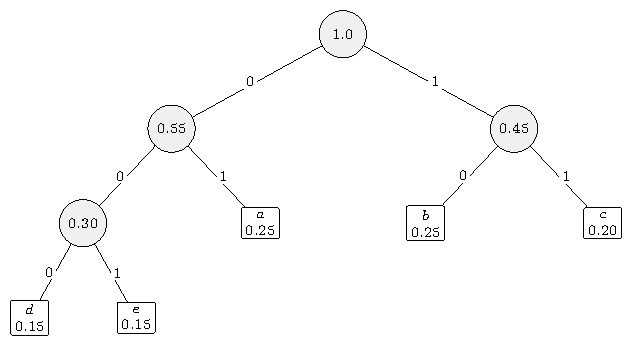
\includegraphics[width=0.72\textwidth]{huffman/huffman-five-symbol-tree}
    \caption{Albero di Huffman per la sorgente con cinque simboli.}
    \label{fig:huffman_five_symbol_tree}
\end{figure}

Infine si fondono i due simboli rimasti, di probabilità $0.45$ e $0.55$, e si risale all'indietro assegnando $0$ e $1$ a ogni biforcazione. Una possibile scelta è rappresentata in \autoref{fig:huffman_five_symbol_tree}: per leggere la parola di codice di un simbolo basta partire dalla radice e concatenare le etichette degli archi incontrati fino alla foglia. Ad esempio, si ottiene il seguente codice:

\begin{center}
    \begin{tabular}{|c|c|c|}
        \hline
        \textbf{Simbolo} & \textbf{Probabilità} & \textbf{Parola di codice} \\ \hline
        $a$              & $0.25$               & \lbox{01}                 \\ \hline
        $b$              & $0.25$               & \lbox{10}                 \\ \hline
        $c$              & $0.20$               & \lbox{11}                 \\ \hline
        $d$              & $0.15$               & \lbox{000}                \\ \hline
        $e$              & $0.15$               & \lbox{001}                \\ \hline
    \end{tabular}
\end{center}

La scelta non è necessariamente unica, soprattutto quando ci sono probabilità uguali; tuttavia qualunque codice ottenuto seguendo correttamente la procedura di Huffman è ottimale.

\paragraph{Esempio con albero di Huffman.}
Consideriamo ora la sorgente:
\[
    S=
    \begin{pmatrix}
        a    & b    & c    & d    & e    & f    & g    \\
        0.05 & 0.05 & 0.10 & 0.20 & 0.30 & 0.20 & 0.10
    \end{pmatrix}
\]
applicando l'algoritmo si ottiene l'albero in \autoref{fig:huffman_example_tree}. Ogni parola di codice si legge seguendo il cammino dalla radice alla foglia: a ogni arco sinistro si associa $0$, mentre a ogni arco destro si associa $1$.

\begin{figure}[htpb]
    \centering
    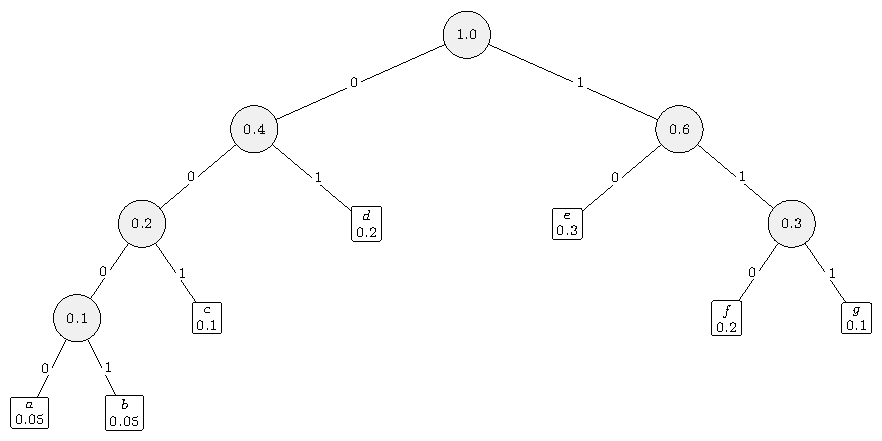
\includegraphics[width=0.82\textwidth]{huffman/huffman-example-tree}
    \caption{Albero di Huffman per una sorgente binaria con sette simboli.}
    \label{fig:huffman_example_tree}
\end{figure}

Leggendo i cammini nell'albero si ottiene:
\begin{center}
    \begin{tabular}{|c|c|c|}
        \hline
        \textbf{Simbolo} & \textbf{Probabilità} & \textbf{Parola di codice} \\ \hline
        $a$              & $0.05$               & \lbox{0000}               \\ \hline
        $b$              & $0.05$               & \lbox{0001}               \\ \hline
        $c$              & $0.10$               & \lbox{001}                \\ \hline
        $d$              & $0.20$               & \lbox{01}                 \\ \hline
        $e$              & $0.30$               & \lbox{10}                 \\ \hline
        $f$              & $0.20$               & \lbox{110}                \\ \hline
        $g$              & $0.10$               & \lbox{111}                \\ \hline
    \end{tabular}
\end{center}

La lunghezza media del codice è:
\[
    L_S(C)
    =
    0.05\cdot4
    +0.05\cdot4
    +0.10\cdot3
    +0.20\cdot2
    +0.30\cdot2
    +0.20\cdot3
    +0.10\cdot3
    =
    2.6.
\]
L'entropia della sorgente vale:
\[
    H(S)=-\sum_i p_i\log_2 p_i \approx 2.5464.
\]
Il codice è quindi molto vicino al limite teorico dato dall'entropia e, essendo stato costruito con l'algoritmo di Huffman, non esiste un altro codice a prefisso binario con lunghezza media inferiore.

\subsubsection{Codifica di Huffman per codici d-ari}
La stessa procedura di costruzione può essere estesa a codici d-ari, con $d>2$. In questo caso, invece di fondere i due simboli meno probabili, si fondono i $d$ simboli meno probabili in un unico simbolo, la cui probabilità è la somma delle probabilità dei simboli fusi. In questo modo, ogni sorgente ridotta avrà $d-1$ simboli rispetto a prima, e si continua a fondere fino ad arrivare a una sorgente con $d$ simboli. Si nota che la sorgente iniziale deve avere almeno $d+\alpha(d-1)$ simboli, dove $\alpha$ è un intero non negativo.

A questo punto, si assegnano i simboli di codice $0,1,\ldots,d-1$ ai simboli rimasti, e si risale all'indietro lungo tutte le fusioni fatte, appendendo a ogni parola di codice i simboli $0,1,\ldots,d-1$ a seconda della posizione del simbolo fuso. Se l'ultima sorgente da ridurre (ovvero la radice dell'albero) ha meno di $d$ simboli, si possono aggiungere simboli fittizi con probabilità $0$ per arrivare al numero desiderato. Dopo la crezione del codice questi simboli fittizi possono essere eliminati.

\paragraph{Esempio d-ario}
Consideriamo la sorgente:
\begin{center}
    \begin{tabular}{|c|c||c|c||c|c|}
        \hline
        \textbf{Simbolo} & \textbf{Prob.} &
        \textbf{Simbolo} & \textbf{Prob.} &
        \textbf{Simbolo} & \textbf{Prob.}                                                                   \\ \hline
        $a$              & $0.22$         & $b$ & $0.15$ & $c$                    & $0.12$                  \\ \hline
        $d$              & $0.10$         & $e$ & $0.10$ & $f$                    & $0.08$                  \\ \hline
        $g$              & $0.06$         & $h$ & $0.05$ & $i$                    & $0.05$                  \\ \hline
        $l$              & $0.04$         & $m$ & $0.03$ & \textcolor{red}{$n,o$} & \textcolor{red}{$0.00$} \\ \hline
    \end{tabular}
\end{center}
Vogliamo costruire un codice quaternario. Notiamo subito che gli 11 simboli presenti non bastano infatti per la formula $11 \neq 4 + \alpha\cdot (4-1)$ per nessun intero $\alpha$. Aggiungiamo quindi due simboli fittizi $n$ e $o$ con probabilità $0$ per arrivare così al numero di simboli necessario. Una possibile sequenza di fusioni, scegliendo ogni volta i quattro simboli meno probabili, è:
\[
    (n,o,m,l) \rightarrow 0.07,
    \quad
    (h,i,g,(n,o,m,l)) \rightarrow 0.23,
    \quad
    (f,d,e,c) \rightarrow 0.40,
\]
\[
    \bigl(b,a,(h,i,g,(n,o,m,l)),(f,d,e,c)\bigr)  \rightarrow 1.00.
\]

\begin{figure}[htpb]
    \centering
    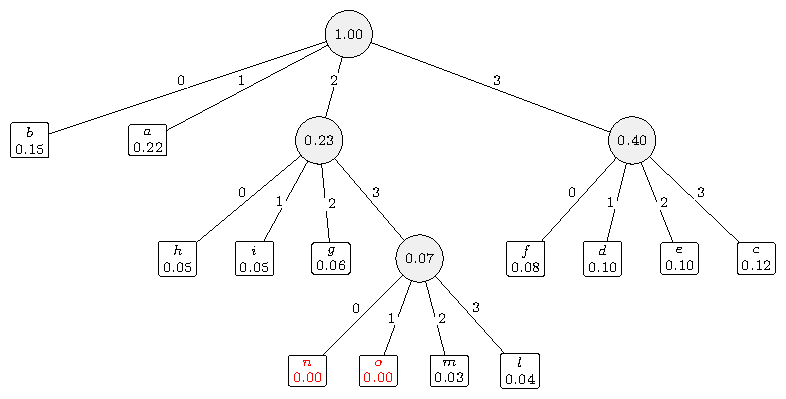
\includegraphics[width=0.95\textwidth]{huffman/huffman-quaternary-example-tree}
    \caption{Albero di Huffman quaternario per la sorgente dell'esempio.}
    \label{fig:huffman_quaternary_example_tree}
\end{figure}

In \autoref{fig:huffman_quaternary_example_tree} le parole di codice si leggono dalla radice alle foglie concatenando le etichette degli archi; i simboli fittizi $n$ e $o$ non fanno parte del codice finale. Quindi otteniamo ad esempio il seguente codice quaternario:

\begin{center}
    \begin{tabular}{|c|c|c|}
        \hline
        \textbf{Simbolo} & \textbf{Probabilità} & \textbf{Parola di codice} \\ \hline
        $a$              & $0.22$               & \lbox{1}                  \\ \hline
        $b$              & $0.15$               & \lbox{0}                  \\ \hline
        $c$              & $0.12$               & \lbox{33}                 \\ \hline
        $d$              & $0.10$               & \lbox{31}                 \\ \hline
        $e$              & $0.10$               & \lbox{32}                 \\ \hline
        $f$              & $0.08$               & \lbox{30}                 \\ \hline
        $g$              & $0.06$               & \lbox{22}                 \\ \hline
        $h$              & $0.05$               & \lbox{20}                 \\ \hline
        $i$              & $0.05$               & \lbox{21}                 \\ \hline
        $l$              & $0.04$               & \lbox{233}                \\ \hline
        $m$              & $0.03$               & \lbox{232}                \\ \hline
    \end{tabular}
\end{center}

\subsubsection{Huffman per un testo in input}
L'algoritmo di Huffman può essere usato anche per costruire un codice ottimale a partire da un testo in input, senza conoscere a priori la distribuzione di probabilità dei simboli. In questo caso, si contano le frequenze di ogni simbolo nel testo e si costruisce la sorgente associata, con probabilità calcolate come frequenza del simbolo diviso la lunghezza totale del testo. A questo punto, si applica l'algoritmo di Huffman alla sorgente così ottenuta per costruire il codice ottimale.

\paragraph{Esempio.}
Dato il testo in input: \texttt{LA BELLA LILLI BALLA} si contano le frequenze dei singoli simboli\footnote{Per semplicità i simboli che vengono considerati sono solo le lettere stesse, altrimenti potrebbero essere contati anche gli spazi, gli accenti e quant'altro.}:
\begin{center}
    \begin{tabular}{|c|c|c|}
        \hline
        \textbf{Simbolo} & \textbf{Frequenza} & \textbf{Probabilità} \\ \hline
        $A$              & 4                  & $4/17$               \\ \hline
        $B$              & 2                  & $2/17$               \\ \hline
        $E$              & 1                  & $1/17$               \\ \hline
        $I$              & 2                  & $2/17$               \\ \hline
        $L$              & 8                  & $8/17$               \\ \hline
    \end{tabular}
\end{center}
solo una volta calcolate le frequenze e le probabilità dei simboli, si può applicare l'algoritmo di Huffman. Allora facendo le seguenti fusioni:
\[
    (E,B) \rightarrow 0.176,
    \qquad
    ((E,B),I) \rightarrow 0.294,
    \qquad
    (A,((E,B),I)) \rightarrow 0.471,
\]
\[
    (L,(A,((E,B),I))) \rightarrow 1.00
\]
ottenendo, per esempio, il codice:
\begin{center}
    \begin{tabular}{|c|c|}
        \hline
        \textbf{Simbolo} & \textbf{Codice} \\ \hline
        $A$              & \lbox{10}       \\ \hline
        $B$              & \lbox{1110}     \\ \hline
        $E$              & \lbox{1111}     \\ \hline
        $I$              & \lbox{110}      \\ \hline
        $L$              & \lbox{0}        \\ \hline
    \end{tabular}
\end{center}
allora il testo di input, senza contare gli spazi, può essere codificato come:
\begin{center}
    \texttt{0 10 1110 1111 0 0 10 0 110 0 0 110 1110 10 0 0 10}
\end{center}
Concatenando le parole di codice si ottiene:
\begin{center}
    \texttt{0101110111100100110001101110100010}
\end{center}
La lunghezza complessiva del messaggio codificato è quindi pari a $34$ bit. Poiché il testo contiene $17$ simboli, la lunghezza media effettivamente ottenuta è:
\[
    \frac{34}{17}=2\quad \texttt{bit/symbol}
\]

La decodifica del messaggio è immediata, basta leggere il messaggio codificato da sinistra a destra e sostituire ogni parola di codice con il simbolo corrispondente. Essendo il codice a prefisso, non ci sono ambiguità: ogni parola di codice è riconoscibile non appena viene letta completamente, senza dover aspettare di leggere ulteriori simboli.

\paragraph{Compression ratio e compression factor.}
Per valutare la compressione si confronta il messaggio compresso con una rappresentazione standard a $8$ bit per carattere, la lunghezza non compressa sarebbe $17\cdot 8 = 136$ bit. Allora il \textbf{compression ratio} è:
\[
    \frac{\text{dimensione del testo compresso}}{\text{dimensione del testo non compresso }}
    =
    \frac{34}{136}
    =
    \frac{1}{4}
    =
    25\%,
\]
mentre il \textbf{compression factor} è il rapporto inverso:
\[
    \frac{\text{dimensione del testo non compresso}}{\text{dimensione del testo compresso}}
    =
    \frac{136}{34}
    =
    4.
\]
Il compression ratio dice quindi quale frazione della dimensione iniziale rimane dopo la compressione; il compression factor dice invece di quante volte il testo compresso è più piccolo rispetto al testo non compresso. In questo esempio, usando il confronto a $8$ bit per carattere, il messaggio occupa il $25\%$ della dimensione iniziale, cioè è $4$ volte più piccolo.

\paragraph{Algoritmo di compressione su un testo in input.}
Nel caso in cui la sorgente non sia nota a priori ma venga ricavata direttamente dal testo, l'applicazione dell'algoritmo di Huffman può essere riassunta nei seguenti passi:
\begin{enumerate}
    \item si legge l'intero testo in input $T$ e si contano le occorrenze $\operatorname{occ}(a)$ di ogni simbolo $a$;
    \item si calcola la probabilità empirica di ogni simbolo:
          \[
              p(a)=\frac{\operatorname{occ}(a)}{|T|};
          \]
    \item si ordinano i simboli in base alla probabilità, oppure si inseriscono direttamente in una coda di priorità;
    \item si costruisce l'albero di Huffman fondendo, a ogni passo, i due nodi con probabilità minore;
    \item quando resta un solo nodo, esso rappresenta la radice dell'albero di Huffman;
    \item si assegna una parola di codice a ogni simbolo leggendo il cammino dalla radice alla foglia corrispondente;
    \item si codifica il testo sostituendo ogni simbolo con la sua parola di codice.
\end{enumerate}
In una compressione reale, oltre al corpo del messaggio compresso, bisogna però conservare anche l'informazione necessaria alla decodifica, cioè l'albero di Huffman oppure una tabella equivalente dei codici. Per questo motivo, quando il testo è molto piccolo, il vantaggio teorico osservato sul solo corpo compresso può essere ridotto o perfino annullato dal costo di memorizzazione della tabella.



\subsubsection{Limiti pratici della codifica di Huffman}
La codifica di Huffman descritta finora è una codifica \textbf{statica}: il codice viene costruito a partire da una distribuzione di probabilità che deve essere nota prima della codifica vera e propria. Quando la distribuzione non è data, ma deve essere dedotta dal testo, è necessario analizzare preliminarmente l'intero input per contare le occorrenze dei simboli e stimare le probabilità empiriche.

Questo significa che la compressione avviene in due fasi distinte:
\begin{enumerate}
    \item \textbf{Costruzione del modello}, in cui si stimano le probabilità dei simboli e si costruisce l'albero di Huffman;
    \item \textbf{Codifica del messaggio}, in cui ogni simbolo del testo viene sostituito dalla parola di codice corrispondente.
\end{enumerate}
Questa distinzione è importante perché la prima fase può richiedere tempo e memoria, soprattutto quando il testo è grande o quando l'alfabeto contiene molti simboli distinti.

Inoltre, per poter decodificare il messaggio, il ricevitore deve conoscere lo stesso codice usato dall'encoder. Per questo motivo, oltre al corpo del messaggio compresso, bisogna memorizzare o trasmettere anche una descrizione del codice usato. In pratica, il file compresso è formato da due parti:
\begin{itemize}
    \item il corpo del messaggio compresso, cioè la sequenza di bit ottenuta concatenando le parole di codice dei simboli del testo;
    \item la tabella dei codici, oppure una rappresentazione equivalente dell'albero di Huffman; questa seconda parte ha dimensione $\mathcal{O}(|A|)$, dove $A$ è l'alfabeto della sorgente.
\end{itemize}
Questa parte introduttiva, cioè il preambolo del file compresso, aumenta la dimensione complessiva del file compresso e può diventare rilevante quando il testo è corto o quando l'alfabeto è grande. Infine, se la tabella o l'albero vengono persi o corrotti, la decompressione può diventare impossibile, perché il flusso di bit non contiene da solo il significato dei simboli originari.

\subsubsection{Complessità e decodifica}
\paragraph{Complessità di costruzione.}
La costruzione dell'albero di Huffman richiede di selezionare ripetutamente i due nodi con probabilità minore. Se si usa una coda di priorità implementata tramite \textbf{min-heap}, e se $n$ indica il numero di simboli distinti della sorgente, il costo complessivo dell'algoritmo è:
\[
    \mathcal{O}(n\log n).
\]
Infatti, a ogni iterazione si estraggono due nodi minimi e si reinserisce il nodo ottenuto dalla loro fusione. Se però i simboli sono già ordinati in base alla probabilità, la costruzione può essere resa lineare usando due code: una per le foglie iniziali e una per i nodi interni generati dalle fusioni.

\paragraph{Decodifica tramite l'albero.}
Una volta noto l'albero di Huffman, la decodifica è concettualmente semplice. Il decoder parte dalla radice dell'albero e legge il messaggio compresso un bit alla volta. Se legge $0$, si sposta verso il figlio sinistro; se legge $1$, si sposta verso il figlio destro. Quando raggiunge una foglia, emette il simbolo associato a quella foglia e torna alla radice per decodificare il simbolo successivo.

Il motivo per cui questa procedura funziona senza separatori tra le parole di codice è che il codice di Huffman è un codice a prefisso. Appena si raggiunge una foglia, la parola di codice letta è completa e non può essere l'inizio di una parola più lunga.

\subsubsection{Decodifica più veloce}
Attraversare l'albero bit per bit è un metodo naturale e facile da descrivere, ma può essere lento in un'implementazione reale. Il decoder deve infatti leggere il file compresso bit dopo bit e, per ogni bit, seguire un puntatore nell'albero. Questo può essere poco efficiente, soprattutto per file grandi o per alfabeti molto ricchi.

Per velocizzare la decodifica si possono usare delle \textbf{lookup table}, cioè tabelle parzialmente decodificate costruite a partire dal codice di Huffman. Invece di leggere un solo bit alla volta, il decoder legge blocchi di $k$ bit, ad esempio $8$ o $16$, e usa il blocco letto come indice di una tabella. L'elemento della tabella può indicare uno o più simboli già decodificati e, se necessario, quale tabella usare per continuare la decodifica.

L'idea si può vedere in questo modo: il flusso compresso viene spezzato in blocchi di lunghezza $k$ e ciascun blocco viene usato per anticipare parte del lavoro che l'attraversamento dell'albero avrebbe svolto passo dopo passo. Il vantaggio è una decodifica più rapida; lo svantaggio è che le tabelle richiedono spazio e devono essere costruite prima dell'inizio della decodifica. Valori più grandi di $k$ aumentano la velocità, ma fanno crescere anche la memoria richiesta e il costo di preparazione delle tabelle.

\subsubsection{Osservazioni su varianza e ridondanza}
A parità di lunghezza media, può essere preferibile un codice con \textbf{varianza minore} nelle lunghezze delle parole di codice, cioè un codice in cui le lunghezze siano meno sbilanciate. Questo aspetto è rilevante nelle applicazioni pratiche, perché molti sistemi di comunicazione o memorizzazione lavorano con buffer di dimensione fissata. Se alcune parole di codice sono molto più lunghe di altre, il flusso compresso può diventare meno regolare da gestire. Quando durante l'algoritmo sono possibili più fusioni equivalenti, scegliere opportunamente quali sottoalberi fondere può aiutare a ottenere codici con varianza più bassa.

La ridondanza dei codici di Huffman può essere studiata anche con bound più precisi\footnote{Esistono bound superiori e inferiori della ridondanza in funzione delle probabilità della sorgente; qui non servono i dettagli tecnici, ma il fenomeno intuitivo che descrivono.}. Qui basta l'idea intuitiva: se la sorgente è molto sbilanciata e un simbolo ha probabilità vicina a $1$, allora l'entropia tende a $0$ perché quasi tutta l'incertezza scompare. Huffman, però, deve comunque assegnare almeno un bit a quel simbolo, quindi la lunghezza media non può scendere altrettanto velocemente e può restare sensibilmente sopra il limite teorico.

\paragraph{Esempio concettuale.}
Consideriamo una sorgente binaria con $p(a)=0.99$ e $p(b)=0.01$. In questo caso l'entropia è molto piccola, perché quasi sempre viene emesso $a$; tuttavia un codice di Huffman binario deve comunque assegnare, ad esempio, $a\mapsto 0$ e $b\mapsto 1$, quindi la lunghezza media resta pari a $1$ bit per simbolo. Questo esempio mostra bene perché, per sorgenti molto sbilanciate, Huffman può essere ottimale tra i codici a prefisso e allo stesso tempo non essere particolarmente vicino all'entropia.

\subsection{Esercizio guidato}
** scrivere questo esercizio guidato che riassume tutte le codifiche fatte fino ad ora **

\subsection{Codifica di Huffman canonica}
Abbiamo già visto come la codifica classica di Huffman ha delle limitazioni, riassumendo:
\begin{itemize}
    \item la struttura ad albero deve essere memorizzata o trasmessa insieme al messaggio compresso, aumentando la dimensione complessiva del file compresso, questa potrebbe occupare una parte molto significativa del file compresso, soprattutto quando il testo è corto o quando l'alfabeto è grande;
    \item la decodifica tramite l'albero, sebbene concettualmente semplice, può risultare lenta, soprattutto per file grandi o per alfabeti molto ricchi, perché il decoder deve leggere il file compresso bit dopo bit e, per ogni bit, seguire un puntatore nell'albero;
    \item il codice ottenuto non è unico: a parità di distribuzione di probabilità possono esistere più alberi di Huffman, e quindi più assegnazioni diverse di parole di codice. Queste assegnazioni possono cambiare nella sequenza di bit associata ai simboli, ma conservano le stesse lunghezze delle parole e quindi la stessa lunghezza media.
\end{itemize}
Per ovviare a queste limitazioni, si può usare una variante della codifica di Huffman chiamata \textbf{codifica canonica di Huffman}, che non usa un albero o delle tabelle per la decodifica, ma si basa solo sulle lunghezze delle parole di codice. Esse sono sufficienti per poter decodificare il messaggio compresso. Questa tecnica è utile quando l'alfabeto è grande e quando la decodifica deve essere molto veloce.

Partendo proprio da questa osservazione, invece di memorizzare l'intero albero di Huffman, si conserva soltanto l'informazione essenziale: la lunghezza della parola di codice associata a ogni simbolo. A partire da queste lunghezze, associate già a determinati simboli, viene poi costruito un codice a prefisso ordinato secondo le seguenti regole standard:
\begin{itemize}
    \item le codewords della stessa lunghezza vengono assegnate in ordine crescente ai simboli, seguendo l'ordine dei simboli stessi\footnote{Ovvero, se $a$ e $b$ sono due simboli con la stessa lunghezza di parola di codice, e se $a$ viene prima di $b$ nell'ordinamento dei simboli, allora la parola di codice di $a$ sarà più piccola (in ordine lessicografico) della parola di codice di $b$.};
    \item in ordine lessicografico, le codewords compaiono anche dalle più lunghe alle più corte.
\end{itemize}

\textbf{Attenzione:} la codifica canonica \uline{non riassegna le lunghezze ai simboli}. Se l'algoritmo di Huffman classico ha stabilito che un simbolo deve avere una parola lunga $2$ bit, quel simbolo continuerà ad avere una parola lunga $2$ bit anche nel codice canonico. Ciò che cambia è soltanto la specifica sequenza di bit assegnata a quel simbolo. In altre parole, la canonizzazione mantiene fissa la corrispondenza:
\[
    \text{simbolo} \longmapsto \text{lunghezza},
\]
e ricostruisce in modo ordinato la corrispondenza:
\[
    \text{simbolo} \longmapsto \text{codewords}.
\]
Questo è essenziale perché le lunghezze determinano la lunghezza media del codice: assegnare una lunghezza diversa a un simbolo cambierebbe il codice ottenuto da Huffman e potrebbe distruggere l'ottimalità.

Il codice ottenuto è equivalente a quello di Huffman dal punto di vista della lunghezza media, ma è molto più comodo da memorizzare e da decodificare. Esempio di codice canonico:
\begin{table}[htpb]
    \centering
    \begin{tabular}{|c|c|}
        \hline
        \textbf{Simbolo} & \textbf{Codifica} \\ \hline
        $a$              & \lbox{000}        \\ \hline
        $b$              & \lbox{001}        \\ \hline
        $c$              & \lbox{010}        \\ \hline
        $d$              & \lbox{011}        \\ \hline
        $e$              & \lbox{10}         \\ \hline
        $f$              & \lbox{11}         \\ \hline
    \end{tabular}
\end{table}

Il vantaggio principale è pratico: in una compressione reale non basta trasmettere il corpo del messaggio compresso, ma bisogna anche permettere al decoder di ricostruire il codice usato. Se si trasmette l'intero albero, il preambolo può diventare costoso, soprattutto quando l'alfabeto è grande. Con la rappresentazione canonica, invece, non è necessario memorizzare la struttura dell'albero con puntatori; è sufficiente memorizzare una lista ordinata di simboli e un array che indica il primo codice disponibile per ogni lunghezza.

\subsubsection{Costruzione del codice canonico}
La costruzione canonica usa tre strutture principali:
\begin{itemize}
    \item $\text{num}[\ell]$, che contiene il numero di simboli codificati con parole di lunghezza $\ell$. Ovvero, conta quanti simboli hanno una parola di codice lunga $\ell$ bit partendo come prima posizione da $\ell=1$ fino alla lunghezza massima $L_{\max}$;
    \item $\text{symb}[\ell]$, che contiene la lista dei simboli aventi parola di codice lunga $\ell$ bit;
    \item $\text{fc}[\ell]$, cioè \emph{firstcode}, che contiene il primo codice canonico (in formato intero decimale) assegnabile ai simboli di lunghezza $\ell$.
\end{itemize}

Una volta noto $\text{fc}[\ell]$, i codici di lunghezza $\ell$ vengono assegnati in modo consecutivo ai simboli presenti in $\text{symb}[\ell]$. Se ad esempio $\text{fc}[3]=1$, allora il primo codice di lunghezza $3$ è $001$; i successivi saranno $010$, $011$, e così via, sempre scritti usando esattamente $3$ bit.

\begin{algorithm}[htpb]
    \caption{Costruzione dell'array $\text{fc}$}
    \label{alg:firstcode}
    \begin{algorithmic}[1]
        \Require $\text{num}[1\ldots L_{\max}]$, dove $\text{num}[\ell]$ conta i simboli con parole lunghe $\ell$ bit
        \Ensure $\text{fc}[1\ldots L_{\max}]$, dove $\text{fc}[\ell]$ è il primo codice canonico di lunghezza $\ell$
        \State $\text{fc}[L_{\max}] \gets 0$
        \For{$\ell \gets L_{\max}-1, L_{\max}-2, \ldots, 1$}
        \State $\text{fc}[\ell] \gets \dfrac{\text{fc}[\ell+1]+\text{num}[\ell+1]}{2}$
        \EndFor
        \State \Return $\text{fc}$
    \end{algorithmic}
\end{algorithm}

\paragraph{Costruzione dell'array firstcode.}
Nel ciclo for, l'indice $\ell$ rappresenta la lunghezza corrente delle parole di codice. La divisione per $2$ corrisponde a uno shift verso destra: si elimina l'ultimo bit a destra e si risale quindi dal livello $\ell+1$ al livello $\ell$ dell'albero.

Si parte dalla lunghezza massima $L_{\max}$ di una codeword. Il primo codice della lunghezza massima viene posto uguale a zero:
\[
    \text{fc}[L_{\max}] = 0.
\]
Questo significa che le parole di codice più lunghe vengono allocate partendo dalla parte più sinistra dell'albero binario, cioè da codici del tipo $000\ldots0$. Risalendo, le altre codewords saranno $000\ldots01$, $000\ldots10$, $000\ldots11$, e così via. Questo significa che l'albero che si viene a creare è sbilanciato a sinistra.

Continuando verso le lunghezze più corte usando la formula:
\[
    \text{fc}[\ell] =
    \frac{\text{fc}[\ell+1]+\text{num}[\ell+1]}{2}.
\]
Il termine $\text{fc}[\ell+1]+\text{num}[\ell+1]$ rappresenta il primo codice non ancora usato tra quelli lunghi $\ell+1$ bit. Dividere per $2$ equivale a eliminare il bit più a destra, cioè a risalire di un livello nell'albero. In altre parole, si prende il padre del primo nodo libero al livello successivo.

\paragraph{Esempio.}
Consideriamo le lunghezze:
\[
    |d|=|e|=2,\qquad
    |c|=|f|=|g|=3,\qquad
    |a|=|b|=4.
\]
Allora:
\begin{align*}
    \text{num}  & =[0,2,3,2]                          \\
    \text{symb} & =[\emptyset, (d,e), (c,f,g), (a,b)]
\end{align*}
dove le posizioni degli array partono da $1$, invece che da $0$. Invece, nelle liste dei simboli le posizioni partono da $0$, quindi $\text{symb}[2][0]=d$, $\text{symb}[2][1]=e$, $\text{symb}[3][0]=c$, e così via.

Si parte da:
\[
    \text{fc}[4]=0.
\]
Quindi:
\begin{align*}
    \text{fc}[3] & = \frac{\text{fc}[4]+\text{num}[4]}{2}
    = \frac{0+2}{2}=1,                                    \\
    \text{fc}[2] & = \frac{\text{fc}[3]+\text{num}[3]}{2}
    = \frac{1+3}{2}=2,                                    \\
    \text{fc}[1] & = \frac{\text{fc}[2]+\text{num}[2]}{2}
    = \frac{2+2}{2}=2.
\end{align*}
Quindi:
\[
    \text{fc}=[2,2,1,0].
\]

\textbf{NB:} Il valore $\text{fc}[1]=2$ sembra impossibile, perché con un solo bit si possono rappresentare solo i valori $0$ e $1$. Infatti non è un vero codice: è un valore sentinella usato nella decodifica per indicare che non esistono parole valide di lunghezza $1$ e che quindi bisogna leggere almeno un altro bit.

\medskip

I codici canonici si ottengono scrivendo ogni valore con il numero corretto di bit e assegnando parole consecutive ai simboli della stessa lunghezza, nell'ordine fissato.

I simboli con parola di codice lunga $4$ bit sono $a$ e $b$, le cui lunghezze sono state ricavate dall'algoritmo di Huffman classico. Poiché $\text{fc}[4]=0$, il primo codice di lunghezza $4$ è $0000$; il successivo, ottenuto incrementando il valore di uno, è $0001$.

Allo stesso modo, i simboli con parola lunga $3$ bit sono $c$, $f$ e $g$. Partendo da $\text{fc}[3]=1$, cioè da $001$ scritto su $3$ bit, si assegnano consecutivamente i codici $001$, $010$ e $011$. Infine, i simboli con parola lunga $2$ bit sono $d$ ed $e$: partendo da $\text{fc}[2]=2$, cioè da $10$ scritto su $2$ bit, si ottengono $10$ e $11$. Non essendoci simboli di lunghezza $1$ bit, a quella lunghezza non viene assegnata alcuna parola di codice. Il risultato finale è:
\[
    \begin{array}{c|c|c}
        \text{Simbolo} & \text{Lunghezza} & \text{Codice canonico} \\
        \hline
        a              & 4                & \lbox{0000}            \\
        b              & 4                & \lbox{0001}            \\
        c              & 3                & \lbox{001}             \\
        f              & 3                & \lbox{010}             \\
        g              & 3                & \lbox{011}             \\
        d              & 2                & \lbox{10}              \\
        e              & 2                & \lbox{11}
    \end{array}
\]
Il codice ottenuto è ancora un codice a prefisso: nessuna parola è prefisso di un'altra. Questo accade perché l'algoritmo assegna i nodi liberi dell'albero in modo ordinato, da sinistra verso destra, evitando di scegliere un nodo che sia antenato di una parola già assegnata.

\subsubsection{Decodifica del codice canonico}
La decodifica canonica non attraversa l'albero bit per bit. Il decoder legge progressivamente i bit e mantiene:
\begin{itemize}
    \item $v$, il valore numerico dei bit letti fino a quel momento;
    \item $\ell$, la lunghezza corrente.
\end{itemize}

\begin{algorithm}[htpb]
    \caption{Decodifica di una parola canonica}
    \label{alg:canonical_decoding}
    \begin{algorithmic}[1]
        \Require flusso di bit codificato, array $\text{fc}$, array $\text{symb}$
        \Ensure simbolo decodificato
        \State $v \gets \texttt{next\_bit()}$
        \State $\ell \gets 1$
        \While{$v < \text{fc}[\ell]$}
        \State $v \gets 2v+\texttt{next\_bit()}$
        \State $\ell \gets \ell+1$
        \EndWhile
        \State \Return $\text{symb}[\ell][v-\text{fc}[\ell]]$
    \end{algorithmic}
\end{algorithm}

Finché vale:
\[
    v < \text{fc}[\ell],
\]
il codice letto è ancora troppo piccolo per essere una parola valida di lunghezza $\ell$, quindi si legge un altro bit. Quando invece la condizione diventa falsa, il simbolo è individuato dalla posizione:
\[
    v-\text{fc}[\ell]
\]
nella lista $\text{symb}[\ell]$.

Per esempio, con $\text{fc}=[2,2,1,0]$, la sequenza $011$ viene letta così:
\[
    v = 0 < \text{fc}[1]=2,
\]
quindi si legge un altro bit:
\[
    v = 01_2 = 1 < \text{fc}[2]=2,
\]
quindi si legge ancora:
\[
    v = 011_2=3 \geq \text{fc}[3]=1.
\]
La lunghezza corretta è quindi $\ell=3$ e l'indice nella lista dei simboli di lunghezza $3$ è:
\[
    3-\text{fc}[3]=3-1=2.
\]
Se $\text{symb}[3]=(c,f,g)$, usando indici che partono da zero, il simbolo decodificato è $g$.

\subsubsection{Esempio completo}
Data la seguente sorgente:
\begin{center}
    \begin{tabular}{|c|c|}
        \hline
        \textbf{Simbolo} & \textbf{Probabilità} \\ \hline
        $a$              & $0.25$               \\ \hline
        $b$              & $0.03125$            \\ \hline
        $c$              & $0.03125$            \\ \hline
        $d$              & $0.125$              \\ \hline
        $e$              & $0.25$               \\ \hline
        $f$              & $0.03125$            \\ \hline
        $g$              & $0.03125$            \\ \hline
        $h$              & $0.25$               \\ \hline
    \end{tabular}
\end{center}
trovare un codice di Huffman canonico e decodificare il messaggio compresso $\texttt{00111100000001001}$. Per prima cosa applichiamo l'algoritmo di Huffman classico per trovare le lunghezze delle parole di codice, trovando ad esempio:
\begin{center}
    \begin{tabular}{|c|c|c|}
        \hline
        \textbf{Simbolo} & \textbf{Probabilità} & \textbf{Codice Huffman} \\ \hline
        $a$              & $0.25$               & \lbox{00}               \\ \hline
        $b$              & $0.03125$            & \lbox{11100}            \\ \hline
        $c$              & $0.03125$            & \lbox{11101}            \\ \hline
        $d$              & $0.125$              & \lbox{110}              \\ \hline
        $e$              & $0.25$               & \lbox{01}               \\ \hline
        $f$              & $0.03125$            & \lbox{11110}            \\ \hline
        $g$              & $0.03125$            & \lbox{11111}            \\ \hline
        $h$              & $0.25$               & \lbox{10}               \\ \hline
    \end{tabular}
\end{center}

Da questa tabella si usano soltanto le lunghezze delle parole di codice. Non bisogna riordinare i simboli assegnando, ad esempio, le lunghezze maggiori ai primi simboli della tabella: le lunghezze restano associate agli stessi simboli per cui sono state ottenute con Huffman classico. Quindi $a$, $e$ e $h$ continueranno ad avere lunghezza $2$, $d$ continuerà ad avere lunghezza $3$, mentre $b$, $c$, $f$ e $g$ continueranno ad avere lunghezza $5$. La codifica canonica modifica solo le sequenze di bit, scegliendole in modo ordinato e consecutivo.

Allora:
\begin{align*}
    \text{num}  & =[0        , 3      , 1  , 0        , 4        ]  \\
    \text{symb} & =[\emptyset, (a,e,h), (d), \emptyset, (b,c,f,g)].
\end{align*}

Si costruisce l'array firstcode:
\begin{align*}
    \text{fc}[5] & =0                                     \\
    \text{fc}[4] & = \frac{\text{fc}[5]+\text{num}[5]}{2}
    = \frac{0+4}{2}=2,                                    \\
    \text{fc}[3] & = \frac{\text{fc}[4]+\text{num}[4]}{2}
    = \frac{2+0}{2}=1,                                    \\
    \text{fc}[2] & = \frac{\text{fc}[3]+\text{num}[3]}{2}
    = \frac{1+1}{2}=1,                                    \\
    \text{fc}[1] & = \frac{\text{fc}[2]+\text{num}[2]}{2}
    = \frac{1+3}{2}=2.
\end{align*}
Quindi:
\[
    \text{fc}=[2,1,1,2,0].
\]

Una volta noto $\text{fc}$, si assegnano i codici canonici partendo dal primo codice disponibile per ogni lunghezza. I simboli di lunghezza $2$ sono $a$, $e$ e $h$: poiché $\text{fc}[2]=1$, i codici assegnati sono $01$, $10$ e $11$. Il simbolo di lunghezza $3$ è $d$, quindi riceve il codice $001$, che corrisponde a $\text{fc}[3]=1$ scritto su $3$ bit. Infine, i simboli di lunghezza $5$ sono $b$, $c$, $f$ e $g$: partendo da $\text{fc}[5]=0$, si ottengono $00000$, $00001$, $00010$ e $00011$.

Il codice canonico finale è:
\begin{center}
    \begin{tabular}{|c|c|c|c|}
        \hline
        \textbf{Simbolo} & \textbf{Probabilità} & \textbf{Lunghezza} & \textbf{Codice canonico} \\ \hline
        $a$              & $0.25$               & $2$                & \lbox{01}                \\ \hline
        $b$              & $0.03125$            & $5$                & \lbox{00000}             \\ \hline
        $c$              & $0.03125$            & $5$                & \lbox{00001}             \\ \hline
        $d$              & $0.125$              & $3$                & \lbox{001}               \\ \hline
        $e$              & $0.25$               & $2$                & \lbox{10}                \\ \hline
        $f$              & $0.03125$            & $5$                & \lbox{00010}             \\ \hline
        $g$              & $0.03125$            & $5$                & \lbox{00011}             \\ \hline
        $h$              & $0.25$               & $2$                & \lbox{11}                \\ \hline
    \end{tabular}
\end{center}

Decodifichiamo ora il messaggio:
\[
    \texttt{00111100000001001}.
\]
Applichiamo l'algoritmo di decodifica precedente. Ogni volta che viene riconosciuta una parola di codice, il decoder emette il simbolo corrispondente e poi ricomincia dalla posizione successiva del messaggio compresso. Ricordiamo che le liste in $\text{symb}$ sono indicizzate a partire da $0$.

Decodifichiamo ora la stringa bit per bit, applicando l'algoritmo canonico.

\begin{itemize}
    \item All'inizio leggiamo \texttt{001}. Dopo il primo bit abbiamo $v=0$ e $\ell=1$:
          poiché $0<\text{fc}[1]=2$, il prefisso non è ancora completo. Leggiamo allora
          un secondo bit, ottenendo ancora $v=0$ e $\ell=2$; anche in questo caso
          $0<\text{fc}[2]=1$, quindi continuiamo. Con il terzo bit si ottiene
          $v=1$ e $\ell=3$. Ora $1\not<\text{fc}[3]=1$, quindi l'algoritmo si ferma.
          L'indice del simbolo è
          \[
              1-\text{fc}[3]=0,
          \]
          e il simbolo corrispondente è $d$.

    \item I bit successivi sono \texttt{11}. Dopo il primo bit si ha $v=1$ e $\ell=1$;
          poiché $1<\text{fc}[1]=2$, serve ancora un bit. Leggendo il secondo bit si ottiene
          $v=3$ e $\ell=2$. A questo punto $3\not<\text{fc}[2]=1$, quindi il codice è
          terminato. L'indice è
          \[
              3-\text{fc}[2]=2,
          \]
          che corrisponde al simbolo $h$.

    \item Procedendo allo stesso modo, la parola \texttt{10} viene letta come segue:
          dopo il primo bit $v=1$ e $\ell=1$, quindi $1<\text{fc}[1]=2$ e si deve
          continuare; dopo il secondo bit $v=2$ e $\ell=2$, e poiché
          $2\not<\text{fc}[2]=1$ l'algoritmo si arresta. L'indice è
          \[
              2-\text{fc}[2]=1,
          \]
          perciò il simbolo decodificato è $e$.

    \item La parola seguente è \texttt{00000}. Finché si leggono i primi quattro bit,
          il valore $v$ rimane uguale a zero e le condizioni
          \[
              0<\text{fc}[1],\qquad
              0<\text{fc}[2],\qquad
              0<\text{fc}[3],\qquad
              0<\text{fc}[4]
          \]
          sono tutte soddisfatte. Dopo il quinto bit, invece, si ha $\ell=5$ e
          $\text{fc}[5]=0$, quindi
          \[
              0\not<\text{fc}[5]=0.
          \]
          Il codice termina e l'indice è
          \[
              0-\text{fc}[5]=0.
          \]
          Il simbolo corrispondente è $b$.

    \item Restano poi i bit \texttt{01}. Dopo il primo bit si ha $v=0$ e $\ell=1$,
          con $0<\text{fc}[1]=2$, quindi si legge ancora un bit. Dopo il secondo bit
          si ottiene $v=1$ e $\ell=2$; siccome $1\not<\text{fc}[2]=1$, il codice è
          completo. L'indice è
          \[
              1-\text{fc}[2]=0,
          \]
          e il simbolo ottenuto è $a$.

    \item Infine si incontra di nuovo la parola \texttt{001}, che viene decodificata
          come prima nel simbolo $d$.
\end{itemize}

La segmentazione ottenuta dall'algoritmo è quindi:
\[
    \texttt{001}\;\texttt{11}\;\texttt{10}\;\texttt{00000}\;\texttt{01}\;\texttt{001},
\]
che corrisponde a:
\[
    d\;h\;e\;b\;a\;d.
\]
Il messaggio decodificato è dunque:
\[
    \texttt{dhebad}.
\]

\subsubsection{Osservazioni}
Il risparmio ottenuto attraverso l'uso del codice canonico è significativo, a maggior ragione quando l'alfabeto è grande. Invece di dover memorizzare o trasmettere un albero con puntatori, è sufficiente memorizzare le lunghezze delle parole di codice e costruire il codice canonico in modo ordinato. Infatti, l'array $\text{num}$ serve durante la costruzione di $\text{fc}$, ma non deve essere salvato nel file compresso: per trasmettere la codifica canonica è sufficiente inviare gli array $\text{fc}$ e $\text{symb}$. Questo significa che:
\begin{itemize}
    \item per l'array $\text{fc}$ servono al massimo $L_{\max}^2$ bit, perché ci sono al più $L_{\max}$ valori di \emph{firstcode} e ciascuno può essere rappresentato con al più $L_{\max}$ bit;
    \item per l'array $\text{symb}$ servono al massimo $(|A| + L_{\max})\log_2(|A|+1)$ bit, dove $|A|$ è la dimensione dell'alfabeto: la struttura contiene complessivamente i $|A|$ simboli della sorgente, più l'informazione necessaria a separare le liste associate alle diverse lunghezze.
\end{itemize}

Il punto importante è che non bisogna memorizzare la struttura dell'albero tramite puntatori. Il risparmio rispetto alla rappresentazione esplicita dell'albero è quindi dell'ordine di:
\[
    \Theta(|A|\log_2(|A|+1)).
\]

Questa osservazione va letta insieme al limite generale dei codici di Huffman: se l'entropia della sorgente è molto grande, il possibile bit in più rispetto all'entropia diventa trascurabile. Se invece la sorgente è molto sbilanciata, Huffman resta limitato dal fatto che un codice a prefisso binario non può rappresentare un simbolo usando meno di $1$ bit. Perciò, se i simboli dell'alfabeto $A$ sono rappresentati originariamente con parole fisse di lunghezza $\log_2 |A|$, il rapporto tra dimensione compressa e dimensione originale non può scendere sotto:
\[
    \frac{1}{\log_2 |A|}.
\]
Nel caso del codice ASCII, in cui $|A|=256$, si ottiene $\log_2 |A|=8$: quindi Huffman non può comprimere un testo fino a occupare meno di $\frac{1}{8}$ della dimensione originale, cioè circa il $12{,}5\%$.

\subsection{Codifica di Huffman adattiva}
La codifica di Huffman vista finora è una codifica \textbf{statica}: prima si conosce o si stima la distribuzione dei simboli, poi si costruisce l'albero e infine si codifica il testo. Questo approccio funziona bene quando la sorgente è nota, ma richiede una fase preliminare di analisi oppure la trasmissione di informazioni aggiuntive, come le probabilità, l'albero o una tabella equivalente.

La \textbf{codifica di Huffman adattiva} elimina questa assunzione: non richiede di conoscere in anticipo le probabilità dei simboli. L'albero viene costruito e aggiornato dinamicamente mentre il testo viene letto. In questo modo il codice usato in un certo istante dipende soltanto dalla porzione di messaggio già osservata.

\subsubsection{Idea intuitiva}
L'idea di base è costruire, passo dopo passo, un albero di Huffman che sia adatto alla parte di messaggio già codificata. Dopo ogni simbolo letto, le frequenze vengono aggiornate e, se necessario, l'albero viene riorganizzato per conservare le proprietà tipiche di un albero di Huffman: i simboli più frequenti devono tendere a stare più vicini alla radice, mentre quelli meno frequenti possono stare più in profondità.

All'inizio l'albero può essere vuoto oppure contenere soltanto un nodo speciale, indicato con \textbf{NYT} (\emph{Not Yet Transmitted}), che rappresenta tutti i simboli non ancora comparsi nel testo. Questo nodo è necessario perché, quando arriva un simbolo nuovo, il decoder deve capire che non può ancora cercarlo nell'albero corrente.

\begin{algorithm}[htpb]
    \caption{Schema della codifica di Huffman adattiva}
    \label{alg:adaptive_huffman}
    \begin{algorithmic}[1]
        \Require testo in input, alfabeto $A$
        \Ensure flusso di bit compresso
        \State inizializza l'albero con il solo nodo NYT
        \For{ogni simbolo $a$ del testo}
        \If{$a$ è già presente nell'albero}
        \State emetti la parola di codice corrente di $a$
        \Else
        \State emetti la parola di codice corrente del nodo NYT
        \State emetti una rappresentazione esplicita di $a$
        \State sostituisci il nodo NYT con un nodo interno avente come figli un nuovo NYT e il simbolo $a$
        \EndIf
        \State incrementa la frequenza di $a$ e dei suoi antenati
        \State riorganizza l'albero, se necessario, per mantenere le proprietà di Huffman
        \EndFor
    \end{algorithmic}
\end{algorithm}

Quando un simbolo è già apparso, quindi, viene codificato usando la parola di codice che possiede nell'albero corrente. Quando invece il simbolo è nuovo, si trasmette prima il codice del nodo NYT e poi il simbolo stesso in forma esplicita, ad esempio con una codifica fissa concordata sull'alfabeto. Subito dopo, il simbolo viene inserito nell'albero con frequenza iniziale pari a $1$.

La decodifica funziona in modo sincronizzato con la codifica. Il decoder parte dallo stesso albero iniziale e aggiorna l'albero dopo ogni simbolo decodificato seguendo esattamente le stesse regole dell'encoder. Per questo motivo non è necessario trasmettere l'intero albero: encoder e decoder lo ricostruiscono nello stesso modo, passo dopo passo.

\subsubsection{Vantaggi e svantaggi}
La codifica adattiva usa una stima variabile delle probabilità dei simboli: all'inizio le frequenze sono povere, ma diventano più rappresentative man mano che il testo viene letto. Questo porta alcuni vantaggi pratici:
\begin{itemize}
    \item non serve una scansione preliminare del testo per calcolare tutte le frequenze;
    \item non è necessario trasmettere all'inizio l'albero di Huffman statico o la tabella delle probabilità;
    \item viene sfruttata meglio la \textbf{località} del testo, cioè il fatto che in certe zone del messaggio alcuni simboli possano comparire con frequenza temporaneamente alta.
\end{itemize}

Il vantaggio della località si vede bene in un caso semplice: se il messaggio inizia con una sequenza di caratteri che poi non si ripetono più, in una codifica statica questi caratteri risultano rari sul testo complessivo e quindi finiscono molto in basso nell'albero. Nella codifica adattiva, invece, i simboli vengono inseriti e usati subito rispetto al contesto corrente; solo in seguito, se altri simboli diventano più frequenti, verranno spinti più in profondità.

Il prezzo da pagare è che la codifica adattiva non sempre usa meno bit della codifica statica calcolata sull'intero testo. Se si ignora il costo del preambolo, cioè il costo necessario a trasmettere probabilità, albero o tabella, Huffman statico può risultare migliore perché conosce già la distribuzione finale. Tuttavia, se si considera anche questo overhead, la codifica adattiva diventa spesso competitiva: usa un solo passaggio sul testo e non deve allegare al file compresso una descrizione completa del modello.

\subsubsection{Osservazione sui compressori universali}
La codifica adattiva migliora la flessibilità del modello, ma non rende possibile comprimere bene ogni stringa. Non esiste un compressore universale senza perdita che riduca la lunghezza di tutti gli input.

Il motivo è un semplice argomento di conteggio. Le stringhe binarie di lunghezza $n$ sono esattamente $2^n$. Se un compressore senza perdita comprimesse tutte queste stringhe in stringhe più corte di $n$ bit, dovrebbe assegnare a ciascun input una codifica diversa, altrimenti il decoder non potrebbe ricostruire univocamente il messaggio originale. Ma le stringhe binarie di lunghezza minore di $n$ sono:
\[
    1+2+2^2+\cdots+2^{n-1}=2^n-1,
\]
quindi sono meno degli input possibili. Di conseguenza, qualche stringa non può essere compressa. Più in generale, la frazione di stringhe di lunghezza $n$ comprimibili fino a $m$ bit è al più $2^{m-n}$. Ogni compressore, quindi, comprime bene alcuni input, ma ne lascia invariati o ne espande altri.

Questa osservazione prepara il passaggio successivo: la codifica di Huffman è ottimale solo se si resta dentro il suo quadro, cioè con un modello fissato e con parole di codice associate ai singoli simboli. La \autoref{fig:beyond_huffman_arithmetic} riassume le principali vie d'uscita da questi vincoli.

\begin{figure}[htpb]
    \centering
    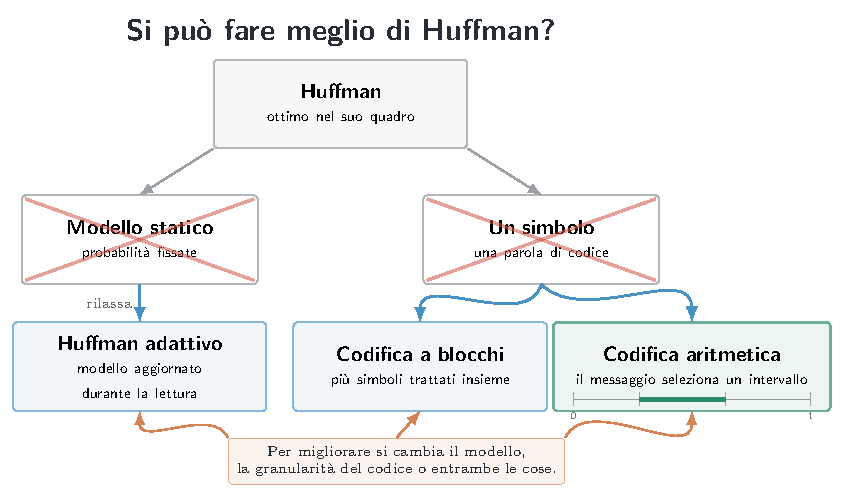
\includegraphics[width=0.92\textwidth]{arithmetic-coding/beyond-huffman}
    \caption{Possibili modi per superare i vincoli entro cui la codifica di Huffman è ottimale: aggiornare il modello, codificare blocchi di simboli o rappresentare l'intero messaggio mediante un intervallo.}
    \label{fig:beyond_huffman_arithmetic}
\end{figure}

\subsection{Codifica aritmetica}
La codifica di Huffman resta ottimale finché si lavora dentro il suo modello: a ogni simbolo viene assegnata una parola di codice intera, e quindi un simbolo non può essere rappresentato con meno di un bit. Questo vincolo diventa molto evidente quando la distribuzione è sbilanciata. Se, ad esempio, una sorgente binaria ha $p(a)=0.99$ e $p(b)=0.01$, l'entropia è:
\[
    H(S)
    =
    0.99\log_2\frac{1}{0.99}
    +
    0.01\log_2\frac{1}{0.01}
    \simeq 0.08056
    \quad \text{bit/simbolo}.
\]
Qualunque codice a prefisso binario sui singoli simboli usa però almeno un bit per ogni simbolo. La \textbf{codifica aritmetica} supera questo limite cambiando punto di vista: non associa una parola di codice a ogni simbolo, ma rappresenta l'intero messaggio come un numero reale in un sottointervallo di $[0,1)$.

L'idea è questa: si parte dall'intervallo $[0,1)$ e, per ogni simbolo letto, lo si suddivide in sottointervalli proporzionali alle probabilità dei simboli. Il sottointervallo corrispondente al simbolo corrente diventa il nuovo intervallo corrente. Alla fine, qualunque numero interno all'intervallo finale identifica l'intero messaggio, purché encoder e decoder condividano lo stesso modello probabilistico e lo stesso ordine dei simboli.

\subsubsection{Bit stream e frazioni dyadiche}
Un bit stream finito $b_1b_2\ldots b_k$ rappresenta la frazione binaria:
\[
    0.b_1b_2\ldots b_k
    =
    \sum_{i=1}^{k} b_i2^{-i}.
\]
Equivalentemente, se $\operatorname{val}(b_1b_2\ldots b_k)$ indica il valore intero della stringa binaria, allora:
\[
    0.b_1b_2\ldots b_k
    =
    \frac{\operatorname{val}(b_1b_2\ldots b_k)}{2^k}.
\]
Le frazioni di questa forma, cioè $v/2^k$, sono dette \textbf{frazioni dyadiche}. Per produrre un output binario, la codifica aritmetica deve quindi scegliere una frazione dyadica contenuta nell'intervallo finale. Più l'intervallo finale è grande, meno bit servono per specificare un suo punto interno; più è piccolo, più bit sono necessari.

In altre parole, quando si parla di frazioni dyadiche il denominatore è sempre una potenza di $2$, per cui la sua conversione binaria è rappresentata da una sequenza di bit finita.

Per convertire un numero reale $x\in[0,1)$ nella sua rappresentazione binaria frazionaria si usa un procedimento molto semplice: si moltiplica ripetutamente per $2$ e, a ogni passo, si guarda se il risultato ha superato oppure no la parte intera $1$. Il bit emesso è proprio quella parte intera.

\begin{algorithm}[htpb]
    \caption{Conversione di un numero frazionario in binario}
    \label{alg:fractional_binary_converter}
    \begin{algorithmic}[1]
        \Require numero reale $x\in[0,1)$
        \Ensure bit stream che rappresenta $x$ alla precisione scelta
        \State $\text{output} \gets \varepsilon$
        \Repeat
        \State $x \gets 2x$
        \If{$x<1$}
        \State $\text{output} \gets \text{output}\mathbin{::}0$
        \Else
        \State $\text{output} \gets \text{output}\mathbin{::}1$
        \State $x \gets x-1$
        \EndIf
        \Until{$x=0$ oppure è stata raggiunta la precisione richiesta}
        \State \Return output
    \end{algorithmic}
\end{algorithm}

Il simbolo $::$ indica la concatenazione di un nuovo bit alla stringa già prodotta. Se durante l'algoritmo si arriva a $x=0$, la rappresentazione binaria è finita: questo è esattamente ciò che accade per le frazioni dyadiche. Se invece il resto non diventa mai zero, la rappresentazione è infinita o periodica, e allora bisogna fermarsi dopo un numero di bit stabilito.

\subsubsection{Algoritmo di codifica}
Sia $A=\{\sigma_1,\ldots,\sigma_m\}$ un alfabeto ordinato. Per ogni simbolo $\sigma\in A$, indichiamo con $p(\sigma)$ la sua probabilità e con:
\[
    F(\sigma)
    =
    \sum_{\tau < \sigma} p(\tau)
\]
la probabilità cumulativa dei simboli che lo precedono nell'ordine fissato. Il simbolo $\sigma$ occupa quindi, nell'intervallo unitario, la porzione:
\[
    [F(\sigma),F(\sigma)+p(\sigma)).
\]

Durante la codifica non è necessario memorizzare continuamente sia l'estremo inferiore sia quello superiore. È spesso più comodo mantenere:
\begin{itemize}
    \item $l_i$, l'estremo inferiore dell'intervallo dopo aver letto i primi $i$ simboli;
    \item $s_i$, la lunghezza dell'intervallo dopo aver letto i primi $i$ simboli.
\end{itemize}
Si inizializza $l_0=0$ e $s_0=1$. Se il simbolo letto al passo $i$ è $S[i]$, allora:
\begin{equation}\label{eq:arithmetic_update_size}
    s_i=s_{i-1}\cdot p(S[i]),
\end{equation}
\begin{equation}\label{eq:arithmetic_update_low}
    l_i=l_{i-1}+s_{i-1}\cdot F(S[i]).
\end{equation}
L'intervallo corrente è quindi:
\[
    I_i=[l_i,l_i+s_i).
\]

\begin{algorithm}[htpb]
    \caption{Codifica aritmetica statica}
    \label{alg:arithmetic_coding}
    \begin{algorithmic}[1]
        \Require sequenza $S=s_1s_2\ldots s_n$, probabilità $p(\sigma)$ e cumulative $F(\sigma)$
        \Ensure un numero dyadico $x\in[l_n,l_n+s_n)$ e la lunghezza $n$
        \State $s_0 \gets 1$
        \State $l_0 \gets 0$
        \For{$i=1,\ldots,n$}
        \State $s_i \gets s_{i-1}\cdot p(S[i])$
        \State $l_i \gets l_{i-1}+s_{i-1}\cdot F(S[i])$
        \EndFor
        \State scegli una frazione dyadica $x\in[l_n,l_n+s_n)$
        \State \Return $\langle x,n\rangle$
    \end{algorithmic}
\end{algorithm}

La lunghezza $n$ è necessaria perché un singolo numero reale non dice da solo quando fermare la decodifica. In alternativa si può aggiungere al modello un simbolo speciale di fine file, spesso indicato come \texttt{EOF}, e fermarsi quando il decoder lo ricostruisce. Il valore $x$ è solitamente l'intervallo inferiore $l_n$, ma si può scegliere qualsiasi frazione dyadica contenuta in $[l_n,l_n+s_n)$.

Un fatto importante segue subito dalla \eqref{eq:arithmetic_update_size}. Dopo $n$ simboli si ha:
\begin{equation}\label{eq:arithmetic_final_size}
    s_n
    =
    \prod_{i=1}^{n} p(S[i]).
\end{equation}
La lunghezza dell'intervallo finale dipende quindi dalle probabilità dei simboli che compaiono nel messaggio, con le loro molteplicità, ma non dall'ordine in cui compaiono. L'ordine cambia la posizione dell'intervallo, non la sua ampiezza.

\subsubsection{Esempio statico: codifica di \texttt{BBBC}}
Consideriamo l'alfabeto $A=\{A,B,C\}$ con:
\[
    p(A)=0.4,\qquad p(B)=0.5,\qquad p(C)=0.1.
\]
Con l'ordine $A<B<C$, l'intervallo unitario viene diviso come:
\[
    A:[0,0.4),\qquad
    B:[0.4,0.9),\qquad
    C:[0.9,1).
\]
Codifichiamo il messaggio \texttt{BBBC}. A ogni passo il sotto intervallo associato al simbolo corrente diventa il nuovo intervallo corrente:
\begin{center}
    \begingroup
    \footnotesize
    \setlength{\tabcolsep}{3pt}
    \renewcommand{\arraystretch}{1.28}
    \begin{tabular}{|c|c|c|c|c|c|}
        \hline
        \textbf{Intervallo corrente}  & \textbf{$A$}          & \textbf{$B$}               & \textbf{$C$}                  & \textbf{Input} & \textbf{Azione} \\ \hline
        $[0,1)$                       & $[0,0.4)$             & $\boldsymbol{[0.4,0.9)}$   & $[0.9,1)$                     & $B$            & Dividi          \\ \hline
        $[0.4,0.9)$                   & $[0.4,0.6)$           & $\boldsymbol{[0.6,0.85)}$  & $[0.85,0.9)$                  & $B$            & Dividi          \\ \hline
        $[0.6,0.85)$                  & $[0.6,0.7)$           & $\boldsymbol{[0.7,0.825)}$ & $[0.825,0.85)$                & $B$            & Dividi          \\ \hline
        $[0.7,0.825)$                 & $[0.7,0.75)$          & $[0.75,0.8125)$            & $\boldsymbol{[0.8125,0.825)}$ & $C$            & Stop            \\ \hline
        $\boldsymbol{[0.8125,0.825)}$ & \multicolumn{5}{c|}{}                                                                                                 \\ \hline
    \end{tabular}
    \endgroup
\end{center}
L'intervallo finale è dunque $[0.8125,0.825)$. Una possibile frazione dyadica contenuta in questo intervallo è:
\[
    0.8125
    =
    \frac{13}{16}.
\]
Convertiamola ora in binario:
\begin{center}
    \begin{tabular}{|c|c|c|c|}
        \hline
        \textbf{Passo} & \textbf{Moltiplicazione} & \textbf{Bit emesso} & \textbf{Nuovo resto} \\ \hline
        $1$            & $0.8125\cdot 2=1.625$    & $1$                 & $0.625$              \\ \hline
        $2$            & $0.625\cdot 2=1.25$      & $1$                 & $0.25$               \\ \hline
        $3$            & $0.25\cdot 2=0.5$        & $0$                 & $0.5$                \\ \hline
        $4$            & $0.5\cdot 2=1.0$         & $1$                 & $0$                  \\ \hline
    \end{tabular}
\end{center}
Quindi:
\[
    0.8125=0.1101_2.
\]
Gli zeri finali dopo la virgola non cambiano il valore, perciò possiamo scrivere anche:
\[
    0.1101_2
    =
    0.1101000_2
    =
    \frac{104}{128}.
\]
La stringa di bit trasmessa è quindi:
\[
    \texttt{1101000}.
\]
Il decoder, conoscendo le probabilità e la lunghezza del messaggio, ripete la stessa suddivisione: il numero $0.8125$ cade prima nel sotto intervallo di $B$, poi ancora in quello di $B$, poi ancora in quello di $B$, e infine in quello di $C$. L'output ricostruito è quindi \texttt{BBBC}.

\subsubsection{Algoritmo di decodifica}
La decodifica è simmetrica rispetto alla codifica. L'encoder usa il simbolo corrente per scegliere il sotto intervallo; il decoder usa il numero trasmesso per capire in quale sotto intervallo cade. Se $x=0.b$ è il numero rappresentato dalla stringa binaria compressa, il decoder parte da $[0,1)$ e ripete la suddivisione per $n$ passi.

\begin{algorithm}[htpb]
    \caption{Decodifica aritmetica statica}
    \label{alg:arithmetic_decoding}
    \begin{algorithmic}[1]
        \Require numero $x$, lunghezza $n$, probabilità $p(\sigma)$ e cumulative $F(\sigma)$
        \Ensure sequenza originale $S$
        \State $S \gets \varepsilon$
        \State $s_0 \gets 1$
        \State $l_0 \gets 0$
        \For{$i=1,\ldots,n$}
        \State trova l'unico simbolo $\sigma$ tale che $x\in[l_{i-1}+s_{i-1}F(\sigma),\,l_{i-1}+s_{i-1}(F(\sigma)+p(\sigma)))$
        \State $S \gets S::\sigma$
        \State $s_i \gets s_{i-1}\cdot p(\sigma)$
        \State $l_i \gets l_{i-1}+s_{i-1}\cdot F(\sigma)$
        \EndFor
        \State \Return $S$
    \end{algorithmic}
\end{algorithm}

La correttezza dipende dalla sincronizzazione tra encoder e decoder. Entrambi devono usare lo stesso ordine dei simboli, le stesse probabilità e la stessa regola di aggiornamento. Se uno di questi elementi cambia, il numero trasmesso viene interpretato rispetto a una partizione diversa e la decodifica non ricostruisce più il messaggio originale.

\subsubsection{Esempio completo: \texttt{abac}}
Consideriamo il messaggio:
\[
    S=\texttt{abac}
\]
con:
\[
    p(a)=\frac{1}{2},
    \qquad
    p(b)=p(c)=\frac{1}{4}.
\]
Con l'ordine $a<b<c$, le probabilità cumulative sono:
\[
    F(a)=0,\qquad F(b)=\frac{1}{2},\qquad F(c)=\frac{3}{4}.
\]
Applicando le formule di aggiornamento si ottiene:
\begin{center}
    \begingroup
    \footnotesize
    \setlength{\tabcolsep}{3pt}
    \renewcommand{\arraystretch}{1.28}
    \begin{tabular}{|c|c|c|c|c|c|}
        \hline
        \textbf{Intervallo corrente} & \textbf{$a$}              & \textbf{$b$}             & \textbf{$c$}                & \textbf{Input} & \textbf{Azione} \\ \hline
        $[0,1)$                      & $\boldsymbol{[0,1/2)}$    & $[1/2,3/4)$              & $[3/4,1)$                   & $a$            & Dividi          \\ \hline
        $[0,1/2)$                    & $[0,1/4)$                 & $\boldsymbol{[1/4,3/8)}$ & $[3/8,1/2)$                 & $b$            & Dividi          \\ \hline
        $[1/4,3/8)$                  & $\boldsymbol{[1/4,5/16)}$ & $[5/16,11/32)$           & $[11/32,3/8)$               & $a$            & Dividi          \\ \hline
        $[1/4,5/16)$                 & $[1/4,9/32)$              & $[9/32,19/64)$           & $\boldsymbol{[19/64,5/16)}$ & $c$            & Stop            \\ \hline
        $\boldsymbol{[19/64,5/16)}$  & \multicolumn{5}{c|}{}                                                                                                 \\ \hline
    \end{tabular}
    \endgroup
\end{center}
L'intervallo finale è:
\[
    \left[\frac{19}{64},\frac{5}{16}\right)
    =
    \left[\frac{38}{128},\frac{40}{128}\right).
\]
Il punto centrale dell'intervallo è:
\[
    \frac{19}{64}+\frac{1}{2}\cdot\frac{1}{64}
    =
    \frac{39}{128}.
\]
Essendo $\frac{39}{128}$ una frazione dyadica, la sua rappresentazione binaria su $7$ bit frazionari è:
\begin{center}
    \begin{tabular}{|c|c|c|c|}
        \hline
        \textbf{Passo} & \textbf{Moltiplicazione} & \textbf{Bit emesso} & \textbf{Nuovo resto} \\ \hline
        $1$            & $39/128\cdot 2=39/64$    & $0$                 & $39/64$              \\ \hline
        $2$            & $39/64\cdot 2=39/32$     & $1$                 & $7/32$               \\ \hline
        $3$            & $7/32\cdot 2=7/16$       & $0$                 & $7/16$               \\ \hline
        $4$            & $7/16\cdot 2=7/8$        & $0$                 & $7/8$                \\ \hline
        $5$            & $7/8\cdot 2=7/4$         & $1$                 & $3/4$                \\ \hline
        $6$            & $3/4\cdot 2=3/2$         & $1$                 & $1/2$                \\ \hline
        $7$            & $1/2\cdot 2=1$           & $1$                 & $0$                  \\ \hline
    \end{tabular}
\end{center}
Quindi:
\[
    \frac{39}{128}
    =
    0.0100111_2.
\]
La codifica può quindi trasmettere:
\[
    \texttt{0100111}.
\]

Vediamo anche la decodifica. Il numero $x=\frac{39}{128}$ rimane fisso: a ogni passo si ridivide l'intervallo corrente e si sceglie il sotto intervallo che contiene $x$.
\begin{center}
    \begingroup
    \scriptsize
    \setlength{\tabcolsep}{2pt}
    \renewcommand{\arraystretch}{1.28}
    \begin{tabular}{|c|c|c|c|c|}
        \hline
        \textbf{Intervallo corrente} & \textbf{$a$}              & \textbf{$b$}             & \textbf{$c$}                & \textbf{Simbolo decodificato} \\ \hline
        $[0,1)$                      & $\boldsymbol{[0,1/2)}$    & $[1/2,3/4)$              & $[3/4,1)$                   & $a$                           \\ \hline
        $[0,1/2)$                    & $[0,1/4)$                 & $\boldsymbol{[1/4,3/8)}$ & $[3/8,1/2)$                 & $b$                           \\ \hline
        $[1/4,3/8)$                  & $\boldsymbol{[1/4,5/16)}$ & $[5/16,11/32)$           & $[11/32,3/8)$               & $a$                           \\ \hline
        $[1/4,5/16)$                 & $[1/4,9/32)$              & $[9/32,19/64)$           & $\boldsymbol{[19/64,5/16)}$ & $c$                           \\ \hline
    \end{tabular}
    \endgroup
\end{center}
In forma discorsiva, la stessa procedura è:
\begin{itemize}
    \item in $[0,1/2)$, quindi il primo simbolo è $a$;
    \item poi, restringendo l'intervallo a $[0,1/2)$, cade in $[1/4,3/8)$, quindi il secondo simbolo è $b$;
    \item poi, restringendo l'intervallo a $[1/4,3/8)$, cade in $[1/4,5/16)$, quindi il terzo simbolo è $a$;
    \item infine cade in $[19/64,5/16)$, quindi il quarto simbolo è $c$.
\end{itemize}
Il messaggio ricostruito è dunque \texttt{abac}.

\subsubsection{Quanti bit servono?}
Dato un intervallo finale $[l,l+s)$, vogliamo scegliere una frazione dyadica interna usando meno bit possibile. Il criterio è scegliere il punto centrale $l+s/2$ e troncarne la rappresentazione binaria a un numero sufficiente di bit.

\begin{theorem}
    Sia $x=0.b_1b_2\ldots$ un numero reale in $[0,1)$ e sia $\operatorname{trunc}_d(x)$ il numero ottenuto mantenendo solo i primi $d$ bit della sua rappresentazione binaria. Allora:
    \[
        \operatorname{trunc}_d(x)\in[x-2^{-d},x].
    \]
\end{theorem}
\begin{proof}
    La differenza tra $x$ e la sua troncatura dipende solo dai bit dopo la posizione $d$:
    \[
        x-\operatorname{trunc}_d(x)
        =
        \sum_{i=1}^{\infty} b_{d+i}2^{-(d+i)}
        \leq
        \sum_{i=1}^{\infty} 2^{-(d+i)}
        =
        2^{-d} \sum_{i=1}^{\infty} 2^{-i} =
        2^{-d}.
    \]
    Inoltre la troncatura non può essere maggiore di $x$, perché sostituisce alcuni bit successivi con zeri. Quindi abbiamo che:
    \[
        x-\operatorname{trunc}_d(x) \leq 2^{-d} \quad \rightarrow \quad x-2^{-d} \leq \operatorname{trunc}_d(x) \leq x.
    \]
\end{proof}

Il punto importante è interpretare la troncatura come un errore controllato. Troncando la rappresentazione binaria a $d$ bit, infatti, non si può ottenere un numero più grande di quello di partenza: si cancellano solo i bit successivi, cioè si sostituisce la coda binaria con zeri. Per questo la troncatura può soltanto spostare il punto verso sinistra.

Il teorema dice inoltre quanto può essere grande questo spostamento. Se il punto di partenza è $x$, allora:
\[
    x-\operatorname{trunc}_d(x)\leq 2^{-d}.
\]
Quindi $2^{-d}$ è una stima del massimo errore possibile quando si conservano solo $d$ bit.

Nel nostro caso scegliamo come punto di partenza il centro dell'intervallo finale:
\[
    x=l+\frac{s}{2}.
\]
Questo punto dista esattamente $s/2$ dal bordo sinistro $l$. Se la troncatura può spostarlo verso sinistra di al massimo $2^{-d}$, allora vogliamo imporre che questo spostamento massimo non superi la distanza dal bordo sinistro:
\[
    2^{-d}\leq \frac{s}{2}.
\]
In questo modo, anche nel caso peggiore, il punto troncato non può uscire dall'intervallo passando sotto $l$.

Risolviamo ora la condizione rispetto a $d$:
\[
    2^{-d}\leq \frac{s}{2}
    \quad\Longleftrightarrow\quad
    2^d\geq \frac{2}{s}
    \quad\Longleftrightarrow\quad
    d\geq \log_2\frac{2}{s}.
\]
Poiché $d$ deve essere un numero intero di bit, scegliamo il più piccolo intero che soddisfa questa disuguaglianza:
\[
    d=\left\lceil\log_2\frac{2}{s}\right\rceil.
\]
Con questa scelta si ha infatti $2^{-d}\leq s/2$, quindi:
\[
    \operatorname{trunc}_d\left(l+\frac{s}{2}\right)
    \geq
    l+\frac{s}{2}-2^{-d}
    \geq
    l+\frac{s}{2}-\frac{s}{2}
    =
    l
\]
e, allo stesso tempo:
\[
    \operatorname{trunc}_d\left(l+\frac{s}{2}\right)
    \leq
    l+\frac{s}{2}
    <
    l+s.
\]
La troncatura cade quindi dentro l'intervallo finale.

\begin{theorem}[Costo della codifica aritmetica]
    Sia $S$ una sequenza di lunghezza $n$ e sia $s_n$ l'ampiezza dell'intervallo finale prodotto dalla codifica aritmetica statica. Il numero di bit sufficienti per rappresentare una frazione dyadica interna all'intervallo finale è al più:
    \[
        2-\sum_{i=1}^{n}\log_2 p(S[i]).
    \]
    Se le probabilità sono stimate dalle frequenze empiriche della sequenza, allora il costo totale è al più:
    \[
        2+nH(S),
    \]
    e quindi il costo medio è al più:
    \[
        H(S)+\frac{2}{n}
        \quad \text{bit/simbolo}.
    \]
\end{theorem}

\begin{proof}
    Dal risultato precedente sappiamo che è sufficiente scegliere:
    \[
        d=\left\lceil\log_2\frac{2}{s_n}\right\rceil
    \]
    bit. Poiché per ogni numero reale $y$ vale $\lceil y\rceil\leq y+1$, otteniamo:
    \[
        d
        =
        \left\lceil\log_2\frac{2}{s_n}\right\rceil
        \leq
        \log_2\frac{2}{s_n}+1
        =
        2-\log_2 s_n.
    \]
    Usando \eqref{eq:arithmetic_final_size}, cioè $s_n=\prod_{i=1}^{n}p(S[i])$, segue:
    \[
        d
        \leq
        2-\log_2\prod_{i=1}^{n}p(S[i])
        =
        2-\sum_{i=1}^{n}\log_2 p(S[i]).
    \]
    Se le probabilità sono stimate dalle frequenze empiriche, cioè $p(\sigma)=n_\sigma/n$, possiamo raggruppare i termini uguali:
    \[
        2-\sum_{i=1}^{n}\log_2 p(S[i])
        =
        2-\sum_{\sigma\in A} n_\sigma \log_2 p(\sigma)
        =
        2+nH(S),
    \]
    dove $n_\sigma$ è il numero di occorrenze di $\sigma$ nella sequenza e, in questo caso, $H(S)$ è l'entropia empirica. Dividendo per $n$ si ottiene il costo medio per simbolo:
    \[
        H(S)+\frac{2}{n}
        \quad \text{bit/simbolo}.
    \]
\end{proof}

Il termine aggiuntivo di due bit è pagato sull'intera sequenza, non su ogni simbolo; per messaggi lunghi il contributo medio $2/n$ diventa quindi trascurabile. Questo è il punto in cui la codifica aritmetica supera il limite pratico di Huffman sui singoli simboli: invece di arrotondare la lunghezza di ogni parola di codice, arrotonda una sola volta il numero che rappresenta l'intero messaggio.

\paragraph{Nota pratica.}
Il vantaggio appena descritto riguarda il numero di bit emessi, non necessariamente la velocità dell'algoritmo. Nelle implementazioni reali, \textbf{Huffman canonico} è spesso più veloce della codifica aritmetica: le parole di codice sono organizzate in modo regolare, quindi encoder e decoder possono usare tabelle di ricerca molto semplici. Inoltre, se si conosce l'inizio di una parola di codice, Huffman permette di decomprimere anche una porzione del file compresso. La codifica aritmetica, invece, rappresenta l'intera sequenza attraverso un unico intervallo finale e il decoder deve ricostruire i simboli in ordine; per questo, di norma, non consente di saltare direttamente a una porzione arbitraria del messaggio. In sintesi: la codifica aritmetica può essere migliore dal punto di vista del rapporto di compressione, mentre Huffman canonico resta spesso più conveniente dal punto di vista computazionale.

\subsubsection{Modello dinamico}
Finora abbiamo considerato un modello statico: le probabilità sono fissate prima di iniziare e restano uguali per tutta la codifica. La codifica aritmetica, però, si presta bene anche a un \textbf{modello dinamico}, in cui le probabilità vengono aggiornate dopo ogni simbolo letto.

Nel modello dinamico encoder e decoder partono dallo stesso modello iniziale e lo aggiornano nello stesso modo. Per esempio, si può partire da un conteggio iniziale uniforme, cioè assegnare una occorrenza fittizia a ogni simbolo dell'alfabeto. Dopo aver codificato o decodificato un simbolo, si incrementa il suo conteggio e si ricalcolano le probabilità. Questo permette al modello di adattarsi localmente al testo, senza conoscere in anticipo l'intera distribuzione.

\paragraph{Esempio dinamico.}
Codifichiamo il messaggio \texttt{bccb} sull'alfabeto $A=\{a,b,c\}$, partendo dai conteggi iniziali:
\[
    \operatorname{occ}(a)=\operatorname{occ}(b)=\operatorname{occ}(c)=1.
\]
All'inizio le probabilità sono tutte $1/3$. Dopo ogni simbolo, il conteggio del simbolo osservato viene incrementato. La tabella va quindi letta riga per riga: le occorrenze indicate sono quelle usate per codificare il simbolo corrente; solo dopo aver scelto il suo sottointervallo il modello viene aggiornato per il passo successivo.
\begin{center}
    \small
    \begin{tabular}{|c|c|c|c|c|}
        \hline
        \textbf{Passo} & \textbf{Simbolo} & \textbf{Occ. prima $(a,b,c)$} & \textbf{Prob. usate $(a,b,c)$} & \textbf{Intervallo scelto} \\ \hline
        $1$            & $b$              & $(1,1,1)$                     & $\left(1/3,1/3,1/3\right)$     & $\left[1/3,2/3\right)$     \\ \hline
        $2$            & $c$              & $(1,2,1)$                     & $\left(1/4,2/4,1/4\right)$     & $\left[7/12,2/3\right)$    \\ \hline
        $3$            & $c$              & $(1,2,2)$                     & $\left(1/5,2/5,2/5\right)$     & $\left[19/30,2/3\right)$   \\ \hline
        $4$            & $b$              & $(1,2,3)$                     & $\left(1/6,2/6,3/6\right)$     & $\left[23/36,13/20\right)$ \\ \hline
    \end{tabular}
\end{center}

\begin{figure}[htpb]
    \centering
    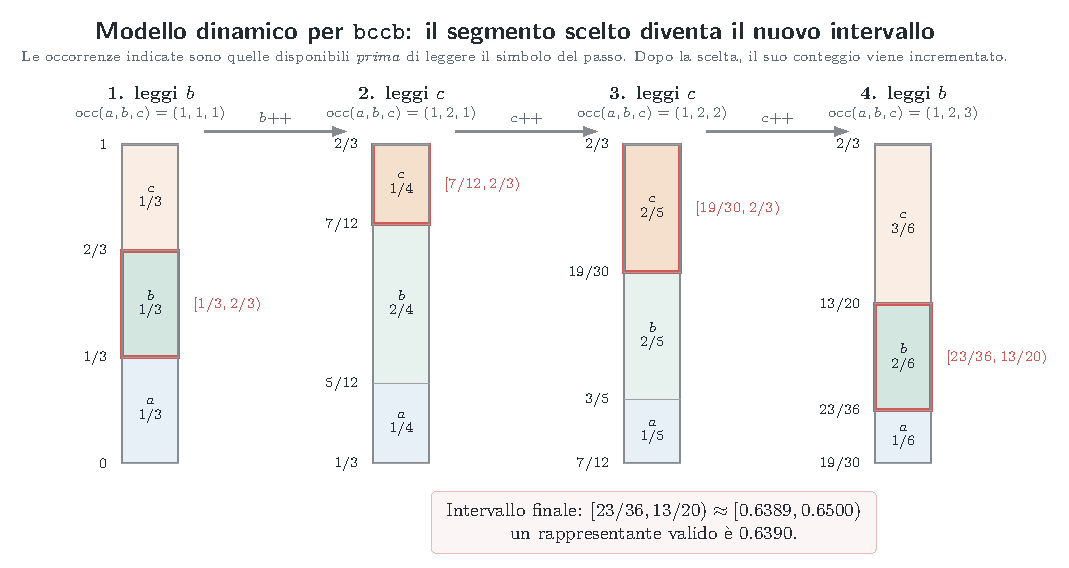
\includegraphics[width=\textwidth]{images/arithmetic-coding/dynamic-model-updates.pdf}
    \caption{Aggiornamento del modello dinamico per la sequenza \texttt{bccb}. Ogni colonna mostra l'intervallo corrente riscalato e suddiviso secondo le occorrenze disponibili prima di leggere il simbolo del passo. Il segmento evidenziato è quello scelto dal simbolo corrente e diventa l'intervallo corrente del passo successivo.}
    \label{fig:arithmetic_dynamic_model_updates}
\end{figure}

La figura mette in evidenza il punto più importante: non cambia solo l'intervallo corrente, cambiano anche le soglie con cui l'intervallo viene suddiviso. Per esempio, dopo aver letto il primo $b$, il conteggio di $b$ passa da $1$ a $2$; per questo, al passo successivo, la parte assegnata a $b$ occupa $2/4$ dell'intervallo corrente invece di $1/3$.

In forma decimale, l'intervallo finale è circa:
\[
    [0.6389,0.6500).
\]
Scegliamo come rappresentante il valore $0.6390$, che cade dentro l'intervallo. Il decoder, partendo dallo stesso modello uniforme, riconosce:
\[
    0.6390\in\left[\frac{1}{3},\frac{2}{3}\right)
    \quad \Rightarrow \quad b.
\]
Poi aggiorna le probabilità, restringe l'intervallo, e trova:
\[
    0.6390\in\left[\frac{7}{12},\frac{2}{3}\right)
    \quad \Rightarrow \quad c.
\]
Continuando con gli stessi aggiornamenti, ricostruisce i simboli successivi $c$ e $b$. L'aspetto essenziale è che il numero trasmesso non cambia: cambia invece, passo dopo passo, la partizione dell'intervallo usata per interpretarlo.

\subsubsection{Aspetti pratici e confronto con Huffman}
La descrizione matematica della codifica aritmetica usa numeri reali e intervalli arbitrariamente piccoli. In una implementazione reale questo non è possibile, quindi si usano versioni a precisione finita. Una variante pratica molto importante è il \textbf{range coding}, matematicamente equivalente alla codifica aritmetica ma implementato con estremi interi e rinormalizzazioni.

Ci sono due problemi pratici da tenere presenti:
\begin{itemize}
    \item il numero finale sarebbe noto solo dopo aver letto tutto l'input; per lavorare in streaming si può dividere il testo in blocchi oppure emettere man mano i prefissi binari comuni agli estremi dell'intervallo corrente;
    \item se l'intervallo diventa molto piccolo, gli estremi richiedono sempre più precisione; per questo le implementazioni confrontano e riscalano periodicamente gli intervalli.
\end{itemize}

Rispetto a Huffman, la codifica aritmetica ha un vantaggio teorico molto forte: può avvicinarsi all'entropia anche quando le probabilità sono molto sbilanciate, perché non è costretta a usare un numero intero di bit per ogni simbolo. D'altra parte, Huffman canonico è più semplice, spesso più veloce, e permette una decodifica più locale: se si conosce un punto di ingresso valido nel flusso compresso, si può ripartire da lì. Nella codifica aritmetica, invece, il significato di un bit dipende dall'intero intervallo corrente, quindi è molto più difficile iniziare la decodifica a metà del flusso.

In pratica, se il modello probabilistico è accurato, la codifica aritmetica può comprimere meglio, specialmente su sorgenti molto sbilanciate o dati come immagini. Se invece il modello è povero o il costo computazionale è prioritario, Huffman resta una scelta robusta e conveniente.

\subsection{Codifica universale degli interi}
Finora abbiamo studiato codici per simboli di una sorgente discreta, assumendo di conoscere o stimare una distribuzione di probabilità. In molti algoritmi di compressione, però, nasce un problema leggermente diverso: bisogna rappresentare una sequenza di \textbf{interi positivi}
\[
    S=s_1,s_2,\ldots,s_n,
    \qquad s_i\in\mathbb{N},\ s_i\geq 1,
\]
senza sapere in anticipo quanto grandi potranno essere gli interi e senza voler trasmettere una tabella di probabilità. L'obiettivo è costruire rappresentazioni binarie:
\begin{itemize}
    \item \textbf{a lunghezza variabile}, così da usare poche cifre per interi piccoli;
    \item \textbf{autolimitanti}, cioè decodificabili senza separatori esterni;
    \item \textbf{a prefisso}, così che la decodifica sia istantanea.
\end{itemize}

La richiesta sugli interi positivi non è davvero restrittiva. Se si vogliono rappresentare anche lo zero e gli interi negativi, si può prima applicare una trasformazione biunivoca verso gli interi positivi, ad esempio:
\begin{equation}\label{eq:integer_positive_mapping}
    z\mapsto
    \begin{cases}
        2z+1, & z\geq 0, \\
        -2z,  & z<0.
    \end{cases}
\end{equation}
In questo modo:
\[
    0\mapsto 1,\quad -1\mapsto 2,\quad 1\mapsto 3,\quad -2\mapsto 4,\quad 2\mapsto 5,\ldots
\]
e qualsiasi codice per interi positivi può essere usato anche per interi con segno.

\paragraph{Dove compare questo problema.}
Un caso molto importante è quello dei motori di ricerca. Per ogni termine $t$ viene memorizzata una lista di documenti in cui $t$ compare. Se i documenti hanno identificativi interi ordinati:
\[
    d_1<d_2<\cdots<d_m,
\]
conviene memorizzare non direttamente gli identificativi, ma i \textbf{gap}
\[
    d_1,\ d_2-d_1,\ d_3-d_2,\ldots,d_m-d_{m-1}.
\]
Questi gap tendono spesso a essere piccoli, quindi un codice a lunghezza variabile può risparmiare molto spazio rispetto a una rappresentazione fissa a $32$ o $64$ bit. Lo stesso tipo di esigenza appare anche in algoritmi come LZ77, LZ78 o in passaggi intermedi di schemi basati su trasformate: il compressore produce interi, e gli interi piccoli sono generalmente più frequenti di quelli grandi.

\subsubsection{Perché il binario semplice non basta}
La rappresentazione binaria naturale di un intero $x$ ha lunghezza:
\[
    |B(x)|=\left\lfloor\log_2 x\right\rfloor+1.
\]
Questa è molto compatta, ma \uline{non è un codice a prefisso}. Per esempio:
\[
    B(1)=\texttt{1},
    \qquad
    B(2)=\texttt{10},
    \qquad
    B(3)=\texttt{11},
    \qquad
    B(4)=\texttt{100},
\]
se si riceve una stringa come \texttt{11011}, non è chiaro dove finisca il primo intero e dove inizi il successivo. Si nota subito come $B(2)$ sia un prefisso di $B(4)$, questo significa che la rappresentazione binaria naturale non può essere usata come codice a prefisso per interi positivi.

Una soluzione semplice, quando si conosce un massimo $m=\max_j s_j$, è usare una rappresentazione fissa di lunghezza:
\begin{equation}\label{eq:fixed_length_integer_code}
    \left\lfloor\log_2 m\right\rfloor+1
\end{equation}
bit per ogni intero. Questo funziona bene se tutti gli interi sono concentrati nello stesso intervallo e hanno dimensioni simili, ma è inefficiente quando molti valori sono piccoli e pochi valori sono grandi. In quel caso il valore massimo costringe tutti gli interi a pagare la stessa lunghezza.

\begin{definizione}
    Un \textbf{codice universale per interi} è un codice binario a prefisso che associa a ogni intero positivo $x$ una parola di codice. Intuitivamente, il codice è universale quando, anche senza conoscere la distribuzione esatta degli interi, assegna a $x$ una lunghezza dell'ordine di $\log x$:
    \[
        l(x)=O(\log x).
    \]
    Nella definizione classica, inoltre, per ogni distribuzione monotona sugli interi, cioè con $p(i)\geq p(i+1)$, la lunghezza media del codice universale resta proporzionale, a meno di una costante, alla lunghezza media di un codice ottimo costruito conoscendo quella distribuzione.
\end{definizione}

L'aggettivo \emph{universale} va quindi letto in questo senso: non si pretende di essere ottimi per una singola distribuzione nota, come accade con Huffman; si vuole invece un codice ragionevolmente vicino al comportamento ottimo per un'intera famiglia di distribuzioni decrescenti, senza dover trasmettere al decoder alcuna tabella di probabilità.

Se la distribuzione è nota sia all'encoder sia al decoder, un codice di Huffman può essere più conveniente. Se invece la distribuzione non è nota con precisione, oppure è nota solo al mittente ma non al ricevente, Huffman richiederebbe anche il costo di comunicare l'albero o le lunghezze delle parole di codice. I codici universali per interi evitano proprio questo costo: \uline{encoder e decoder condividono una regola fissa}.

\subsubsection{Lunghezze ideali e distribuzioni compatibili}
Prima di vedere i codici concreti conviene chiarire il criterio usato. L'idea è la stessa vista con il teorema di Shannon: se un intero $x$ ha probabilità $p(x)$, allora la sua lunghezza ideale dovrebbe essere:
\begin{equation}\label{eq:ideal_integer_code_length}
    l^*(x)=\log_2\frac{1}{p(x)}.
\end{equation}
Questa formula dice che valori più probabili devono avere parole più corte, mentre valori meno probabili possono permettersi parole più lunghe.

\textbf{Parliamo di lunghezze ideali}. Nella pratica le lunghezze di un codice binario devono essere intere e devono anche soddisfare il vincolo di prefisso. Quindi la formula \eqref{eq:ideal_integer_code_length} non produce automaticamente un codice reale, ma descrive il profilo di lunghezze che un codice ottimo dovrebbe cercare di imitare.

Questa formula può essere usata anche al contrario. Se un certo codice assegna lunghezza $l(x)$ all'intero $x$, possiamo chiederci:
\begin{quote}
    Per quale distribuzione di probabilità questa scelta di lunghezze sarebbe naturale?
\end{quote}
Per rispondere si impone:
\[
    l(x)=\log_2\frac{1}{p(x)}
\]
e si risolve rispetto a $p(x)$.

\paragraph{Caso della codifica fissa.}
Se tutti gli interi in $\{1,2,\ldots,m\}$ sono rappresentati con la stessa lunghezza, il codice sta implicitamente trattando tutti i valori come ugualmente probabili. Infatti, se:
\[
    p(x)=\frac{1}{m},
    \qquad x=1,2,\ldots,m,
\]
allora:
\[
    \log_2\frac{1}{p(x)}
    =
    \log_2 m,
\]
che è uguale per ogni $x$. Per questo la codifica fissa è sensata quando i valori sono distribuiti in modo circa uniforme dentro un intervallo noto. Se invece molti valori sono piccoli e pochi sono grandi, la lunghezza fissa spreca spazio sui valori piccoli.

\subsubsection{Codice unario}
Il codice unario è il più semplice codice istantaneo per interi positivi. L'intero $x$ viene rappresentato da $x-1$ zeri seguiti da un uno:
\begin{equation}\label{eq:unary_code}
    U(x)=^{x-1}1.
\end{equation}
I primi valori sono:
\[
    U(1)=\texttt{1},\quad
    U(2)=\texttt{01},\quad
    U(3)=\texttt{001},\quad
    U(4)=\texttt{0001}.
\]
La decodifica è immediata: si contano gli zeri fino al primo $1$. La lunghezza della parola è:
\[
    |U(x)|=x.
\]
Il codice è quindi a prefisso, ma \textbf{non è universale}, perché la sua lunghezza cresce linearmente in $x$ invece che come $\log x$.

\paragraph{Per quale distribuzione è adatto.}
Applichiamo adesso il ragionamento precedente al codice unario. Poiché il codice unario assegna all'intero $x$ una parola di lunghezza $|U(x)|=x$, cerchiamo la distribuzione per cui questa lunghezza coincide con la lunghezza ideale:
\[
    |U(x)|=x=\log_2\frac{1}{p(x)}
\]
risolvendo:
\[
    2^x=\frac{1}{p(x)}
    \quad\Longleftrightarrow\quad
    p(x)=2^{-x}.
\]
Questa è una distribuzione valida sugli interi positivi, perché:
\[
    \sum_{x=1}^{+\infty}2^{-x}=1.
\]
Dunque il codice unario è adatto quando le probabilità decrescono molto rapidamente:
\[
    p(1)=\frac{1}{2},
    \quad
    p(2)=\frac{1}{4},
    \quad
    p(3)=\frac{1}{8},
    \quad
    p(4)=\frac{1}{16},
    \ldots
\]
In questa situazione quasi tutto il peso probabilistico è concentrato sui primi interi, quindi pagare $x$ bit per rappresentare $x$ non è troppo grave. Appena però gli interi grandi diventano abbastanza frequenti, l'unario diventa inefficiente: per rappresentare $1000$ usa $1000$ bit, mentre la rappresentazione binaria naturale ne usa solo $\left\lfloor\log_2 1000\right\rfloor+1=10$.

\subsubsection{Codici di Elias: gamma e delta}
I due codici universali più classici sono i codici di Elias, introdotti da Peter Elias nel 1975: il \textbf{codice gamma} e il \textbf{codice delta}. Entrambi partono da una stessa idea: la rappresentazione binaria di $x$ è compatta, ma non dice dove finisce; allora si codifica anche la sua lunghezza in modo autolimitante.

\paragraph{Codice gamma.}
Sia $B(x)$ la rappresentazione binaria naturale di $x$ e sia:
\[
    N=\left\lfloor\log_2 x\right\rfloor.
\]
Allora $|B(x)|=N+1$, cioè:
\[
    2^N\leq x<2^{N+1}.
\]
Il codice gamma di $x$ è:
\begin{equation}\label{eq:gamma_code}
    \gamma(x)=0^N B(x).
\end{equation}
In altre parole, si scrivono prima $N$ zeri e poi la rappresentazione binaria di $x$ su $N+1$ bit. La lunghezza è:
\begin{equation}\label{eq:gamma_length}
    |\gamma(x)|
    =
    N+(N+1)
    =
    2\left\lfloor\log_2 x\right\rfloor+1.
\end{equation}
Perciò il codice gamma usa circa $2\log_2 x+1$ bit, quindi è universale.

\begin{table}[htpb]
    \centering
    \small
    \begin{tabular}{|l|l|l|}
        \hline
        \textbf{$x$} & \textbf{$B(x)$} & \textbf{$\gamma(x)$} \\ \hline
        $1$          & \texttt{1}      & \texttt{1}           \\ \hline
        $2$          & \texttt{10}     & \texttt{010}         \\ \hline
        $3$          & \texttt{11}     & \texttt{011}         \\ \hline
        $4$          & \texttt{100}    & \texttt{00100}       \\ \hline
        $5$          & \texttt{101}    & \texttt{00101}       \\ \hline
        $6$          & \texttt{110}    & \texttt{00110}       \\ \hline
        $7$          & \texttt{111}    & \texttt{00111}       \\ \hline
        $8$          & \texttt{1000}   & \texttt{0001000}     \\ \hline
        $9$          & \texttt{1001}   & \texttt{0001001}     \\ \hline
    \end{tabular}
    \caption{Primi valori del codice gamma di Elias.}
    \label{tab:gamma_codewords}
\end{table}

\paragraph{Decodifica gamma.}
Per decodificare una parola gamma:
\begin{enumerate}
    \item si contano gli zeri iniziali fino al primo $1$; sia $N$ il loro numero;
    \item il primo $1$ incontrato è il bit più significativo di $B(x)$;
    \item si leggono in totale $N+1$ bit a partire da quel $1$;
    \item la stringa ottenuta viene interpretata come rappresentazione binaria di $x$.
\end{enumerate}

\paragraph{Esempio 1: codifica e decodifica gamma di $9$.}
Poiché:
\[
    9=(1001)_2,
    \qquad
    \left\lfloor\log_2 9\right\rfloor=3,
\]
si scrivono tre zeri seguiti da $1001$:
\[
    \gamma(9)=\texttt{0001001}.
\]
In decodifica, leggendo \texttt{0001001}, si incontrano tre zeri prima del primo $1$, quindi $N=3$. Si leggono allora $N+1=4$ bit a partire dal primo $1$:
\[
    \texttt{1001}_2=9.
\]

L'inefficienza del codice gamma sta nel modo in cui codifica la lunghezza $|B(x)|$: usa una parte unaria, quindi per interi molto grandi questa intestazione diventa costosa. Si può mostrare che il gamma è particolarmente adatto a distribuzioni circa del tipo:
\[
    p(x)\simeq \frac{1}{2x^2}.
\]
Infatti la sua lunghezza è circa $2\log_2 x$, e quindi corrisponde a probabilità proporzionali a $x^{-2}$.

\paragraph{Codice delta.}
Il codice delta migliora il gamma codificando in modo più efficiente la lunghezza di $B(x)$. Sia ancora:
\[
    N=\left\lfloor\log_2 x\right\rfloor,
    \qquad |B(x)|=N+1.
\]
Il codice delta è formato da due parti:
\begin{equation}\label{eq:delta_code}
    \delta(x)=\gamma(N+1)\ \operatorname{tail}(B(x)),
\end{equation}
dove $\operatorname{tail}(B(x))$ indica la rappresentazione binaria di $x$ privata del bit più significativo. Il bit più significativo non serve, perché per un intero positivo è sempre $1$.

La lunghezza è:
\begin{equation}\label{eq:delta_length}
    |\delta(x)|
    =
    |\gamma(N+1)|+N
    =
    2\left\lfloor\log_2(N+1)\right\rfloor+1+N.
\end{equation}
Poiché $N\simeq\log_2 x$, per $x$ grande si ottiene:
\[
    |\delta(x)|
    \simeq
    1+\log_2 x+2\log_2\log_2 x.
\]
Il codice delta è quindi ancora universale, ma per interi grandi è più corto rispetto al codice gamma.

\paragraph{Esempio 2: codifica delta di $14$.}
Per $x=14$ si ha:
\[
    B(14)=\texttt{1110},
    \qquad
    N=\left\lfloor\log_2 14\right\rfloor=3,
    \qquad
    N+1=4.
\]
Ora:
\[
    \gamma(4)=\texttt{00100},
\]
mentre la rappresentazione binaria di $14$ senza il primo bit è:
\[
    \operatorname{tail}(B(14))=\texttt{110}.
\]
Quindi:
\[
    \delta(14)=\texttt{00100}\,\texttt{110}
    =
    \texttt{00100110}.
\]

\paragraph{Decodifica delta.}
Per decodificare una parola delta:
\begin{enumerate}
    \item si decodifica anzitutto una parola gamma iniziale; il risultato è $N+1$;
    \item si calcola $N=(N+1)-1$;
    \item si leggono i successivi $N$ bit;
    \item si antepone un $1$ a questi $N$ bit e si interpreta il risultato in binario.
\end{enumerate}

Per esempio, decodifichiamo:
\[
    \texttt{001010011}.
\]
La parte iniziale \texttt{00101} è una parola gamma:
\[
    \gamma(5)=\texttt{00101}.
\]
Quindi $N+1=5$ e $N=4$. I successivi $4$ bit sono:
\[
    \texttt{0011}.
\]
Anteponendo il bit più significativo si ottiene:
\[
    \texttt{1}\,\texttt{0011}=\texttt{10011}_2=19.
\]
Dunque:
\[
    \delta(19)=\texttt{001010011}.
\]

Anche per il delta si può leggere la lunghezza come indizio della distribuzione per cui il codice è più naturale. Poiché:
\[
    |\delta(x)|\simeq \log_2 x+2\log_2\log_2 x,
\]
il codice delta è adatto a distribuzioni circa del tipo:
\[
    p(x)\simeq \frac{1}{2x(\log x)^2}.
\]

\begin{theorem}[Proprietà di prefisso dei codici gamma e delta]
    I codici $\gamma$ e $\delta$ di Elias sono codici a prefisso, quindi sono istantaneamente decodificabili.
\end{theorem}

\begin{proof}
    Questa dimostrazione non introduce un risultato difficile da imparare a memoria: serve soprattutto a rendere esplicito il motivo per cui la decodifica dei codici di Elias non ha bisogno di separatori esterni.

    Consideriamo prima il codice gamma. Per definizione:
    \[
        \gamma(x)=0^N B(x),
        \qquad
        N=\left\lfloor\log_2 x\right\rfloor.
    \]
    La rappresentazione binaria $B(x)$ ha sempre lunghezza $N+1$ e inizia sempre con $1$. Quando il decoder legge una parola gamma, non conosce ancora $x$, ma può contare gli zeri iniziali. Se incontra $N$ zeri prima del primo $1$, allora sa immediatamente che la parte binaria completa deve essere lunga $N+1$ bit, contando anche quel primo $1$.

    Per esempio, se il flusso inizia con:
    \[
        \texttt{0001001}\ldots
    \]
    il decoder vede tre zeri iniziali, quindi deduce $N=3$. A questo punto non deve indovinare dove termina la parola: deve leggere esattamente $N+1=4$ bit a partire dal primo $1$, cioè:
    \[
        \texttt{1001}.
    \]
    La parola gamma completa è quindi:
    \[
        \texttt{000}\,\texttt{1001}.
    \]
    Tutti i bit successivi appartengono alla parola di codice seguente, non a quella corrente. Questo mostra il punto essenziale: una parola gamma contiene al suo interno l'informazione necessaria per sapere dove finisce.

    Da qui segue la proprietà di prefisso. Se una parola gamma completa potesse essere prefisso di un'altra parola gamma più lunga, il decoder, dopo aver letto la prima parola completa, dovrebbe rimanere incerto se fermarsi oppure continuare. Ma questo non accade: il numero di zeri iniziali determina esattamente quanti bit leggere dopo il primo $1$. Quindi, appena quei bit sono stati letti, la parola è chiusa in modo univoco. Nessuna parola gamma completa può essere prefisso di un'altra.

    Il codice delta usa lo stesso principio, ma in due livelli. Per definizione:
    \[
        \delta(x)=\gamma(N+1)\operatorname{tail}(B(x)),
        \qquad
        N=\left\lfloor\log_2 x\right\rfloor.
    \]
    La prima parte è una parola gamma, quindi, per quanto appena visto, il decoder può riconoscerne la fine in modo univoco. Decodificando questa prima parte ottiene $N+1$, cioè la lunghezza della rappresentazione binaria completa di $x$. A quel punto sa che mancano esattamente $N$ bit, perché il bit più significativo di $B(x)$ è sempre $1$ ed è stato omesso nella seconda parte del delta.

    Anche nel delta, dunque, il decoder sa dove fermarsi: prima legge una parola gamma completa, poi legge un numero fissato di bit successivi. La fine della parola di codice è determinata dalla parola stessa, quindi anche il codice delta è a prefisso.
\end{proof}

\subsubsection{Codice di Fibonacci}
Il codice di Fibonacci usa una struttura diversa. Si basa sul seguente risultato.

\begin{theorem}[Teorema di Zeckendorf]
    Ogni intero positivo può essere rappresentato in modo unico come somma di numeri di Fibonacci distinti, di indice almeno $2$, senza usare due numeri di Fibonacci consecutivi.
\end{theorem}

Usiamo la convenzione:
\[
    F_0=0,\quad
    F_1=1,\quad
    F_2=1,\quad
    F_3=2,\quad
    F_4=3,\quad
    F_5=5,\quad
    F_6=8,\ldots
\]
Per esempio:
\[
    110=89+21.
\]
La rappresentazione alternativa $110=89+13+8$ non è la rappresentazione di Zeckendorf, perché usa due numeri consecutivi, $13$ e $8$.

Formalmente, se:
\begin{equation}\label{eq:zeckendorf_representation}
    N=\sum_{i=0}^{k-1} d_i F_{i+2},
    \qquad d_i\in\{0,1\},
\end{equation}
e l'ultima cifra usata nella rappresentazione è $d_{k-1}=1$, il codice di Fibonacci è:
\begin{equation}\label{eq:fibonacci_code}
    \operatorname{Fib}(N)=d_0d_1\cdots d_{k-1}1.
\end{equation}
L'ultimo $1$ non rappresenta un numero di Fibonacci: è un bit aggiuntivo di terminazione.
Nella rappresentazione di Zeckendorf non compaiono mai due $1$ consecutivi. Aggiungendo un $1$ finale, ogni parola di codice termina invece con la sotto stringa \texttt{11}. Poiché \texttt{11} non può comparire all'interno della rappresentazione, il decoder riconosce la fine della parola appena vede due $1$ consecutivi. Per questo il codice è a prefisso.

\paragraph{Algoritmo di codifica.}
Il passaggio da fissare è la scelta iniziale: alla prima iterazione si prende il massimo numero di Fibonacci $F_j$ tale che $F_j\leq N$. In altre parole, se $N$ non è esso stesso un numero di Fibonacci, si prende il termine della sequenza immediatamente precedente a $N$. Dopo la sottrazione, la stessa regola si applica al resto corrente.

\begin{algorithm}[htpb]
    \caption{Codifica di Fibonacci di un intero positivo}
    \label{alg:fibonacci_encoding}
    \begin{algorithmic}[1]
        \Require intero positivo $N$
        \Ensure parola di codice $\operatorname{Fib}(N)$
        \State $r \gets N$
        \State inizializza tutti i bit $d_i$ a $0$
        \While{$r>0$}
        \State trova il massimo indice $j\geq 2$ tale che $F_j\leq r$
        \State $d_{j-2}\gets 1$
        \State $r\gets r-F_j$
        \EndWhile
        \State sia $k$ tale che $d_{k-1}$ sia l'ultimo bit uguale a $1$
        \State \Return $d_0d_1\cdots d_{k-1}1$
    \end{algorithmic}
\end{algorithm}

\begin{table}[htpb]
    \centering
    \small
    \begin{tabular}{|c|c|c|}
        \hline
        \textbf{$N$} & \textbf{Rappresentazione di Zeckendorf} & \textbf{Codice di Fibonacci} \\ \hline
        $1$          & $F_2$                                   & \texttt{11}                  \\ \hline
        $2$          & $F_3$                                   & \texttt{011}                 \\ \hline
        $3$          & $F_4$                                   & \texttt{0011}                \\ \hline
        $4$          & $F_2+F_4$                               & \texttt{1011}                \\ \hline
        $5$          & $F_5$                                   & \texttt{00011}               \\ \hline
        $6$          & $F_2+F_5$                               & \texttt{10011}               \\ \hline
        $7$          & $F_3+F_5$                               & \texttt{01011}               \\ \hline
        $8$          & $F_6$                                   & \texttt{000011}              \\ \hline
        $9$          & $F_2+F_6$                               & \texttt{100011}              \\ \hline
    \end{tabular}
    \caption{Primi valori del codice di Fibonacci.}
    \label{tab:fibonacci_codewords}
\end{table}

\paragraph{Esempio 3: codifica di Fibonacci di $73$.}
Seguendo l'algoritmo, il primo termine scelto non è un Fibonacci qualsiasi: è il massimo termine della sequenza che non supera $73$, cioè $F_{10}=55$. A ogni passo si ripete la stessa scelta sul resto corrente:
\[
    \begin{aligned}
        73 & \xrightarrow{\;F_{10}=55\;} 18, \\
        18 & \xrightarrow{\;F_7=13\;} 5,     \\
        5  & \xrightarrow{\;F_5=5\;} 0.
    \end{aligned}
\]
Dunque la decomposizione di Zeckendorf è:
\[
    73=55+13+5
    =
    F_{10}+F_7+F_5.
\]
Le posizioni del codice corrispondono, da sinistra a destra, ai coefficienti di:
\[
    F_2,F_3,F_4,F_5,F_6,F_7,F_8,F_9,F_{10}.
\]
Quindi mettiamo $1$ nelle posizioni associate a $F_5$, $F_7$ e $F_{10}$:
\[
    d_0d_1\cdots d_8=\texttt{000101001},
\]
come è stato detto in precedenza, si parte da $i=2$ quindi $d_0=F_2$ e così via. Aggiungendo il bit finale di terminazione:
\[
    \operatorname{Fib}(73)=\texttt{0001010011}.
\]

La decodifica è altrettanto diretta: si rimuove l'ultimo $1$, si associa ai bit rimanenti la sequenza:
\[
    1,2,3,5,8,13,21,34,55,\ldots
\]
e si sommano i valori in corrispondenza dei bit uguali a $1$.

Per esempio:
\[
    \texttt{100011}
\]
termina con \texttt{11}. Rimuovendo l'ultimo $1$ resta:
\[
    \texttt{10001}.
\]
I bit $1$ corrispondono a $F_2=1$ e $F_6=8$, quindi:
\[
    1+8=9.
\]

Il codice di Fibonacci è universale: si può dimostrare che l'intero $x$ viene rappresentato usando al più:
\begin{equation}\label{eq:fibonacci_length_bound}
    1+\log_{\varphi}\left(\sqrt{5}\,x\right)
\end{equation}
bit, dove:
\[
    \varphi=\frac{1+\sqrt{5}}{2}\simeq 1.61803
\]
è il rapporto aureo. Inoltre è un codice \textbf{sincronizzante}: la sotto stringa \texttt{11} permette di riconoscere il confine della parola di codice. Questo è utile in presenza di errori, perché dopo una corruzione locale il decoder può ritrovare un punto di allineamento leggendo fino al successivo terminatore.

\begin{theorem}[Universalità dei codici gamma, delta e Fibonacci]
    I codici gamma, delta e Fibonacci rappresentano ogni intero positivo $x$ usando $O(\log x)$ bit.
\end{theorem}

\begin{proof}
    Per il codice gamma, da \eqref{eq:gamma_length}:
    \[
        |\gamma(x)|
        =
        2\left\lfloor\log_2 x\right\rfloor+1
        =
        O(\log x).
    \]
    Per il codice delta, da \eqref{eq:delta_length}:
    \[
        |\delta(x)|
        =
        \left\lfloor\log_2 x\right\rfloor
        +
        2\left\lfloor\log_2\left(\left\lfloor\log_2 x\right\rfloor+1\right)\right\rfloor
        +
        1.
    \]
    Il termine dominante è $\log_2 x$, mentre $\log_2\log_2 x$ cresce più lentamente; dunque anche $|\delta(x)|=O(\log x)$. Per Fibonacci, il limite \eqref{eq:fibonacci_length_bound} è logaritmico in $x$, quindi anche quel codice è universale.
\end{proof}

\subsubsection{Codici di Rice}
I \textbf{codici di Rice} sono codici per interi molto usati in compressione audio e immagine, ma vanno distinti dai codici universali in senso stretto: per un parametro fissato, la lunghezza di un codice di Rice può crescere linearmente con $x$. Sono però estremamente utili quando gli interi sono concentrati attorno a un valore caratteristico e si vuole una decodifica veloce.

Un codice di Rice dipende da un intero $k\geq 0$. Dato $x\geq 1$, si definiscono:
\begin{equation}\label{eq:rice_parameters}
    q=\left\lfloor\frac{x-1}{2^k}\right\rfloor,
    \qquad
    r=x-2^kq-1.
\end{equation}
Il resto $r$ appartiene all'intervallo:
\[
    0\leq r<2^k,
\]
quindi può essere rappresentato con esattamente $k$ bit. Il codice di Rice è formato da:
\[
    R_k(x)=U(q+1)\ \operatorname{bin}_k(r),
\]
dove $U(q+1)$ è il codice unario di $q+1$ e $\operatorname{bin}_k(r)$ è la rappresentazione binaria di $r$ su $k$ bit. La lunghezza totale è:
\begin{equation}\label{eq:rice_length}
    |R_k(x)|=q+k+1.
\end{equation}

\paragraph{Esempio 4: codice di Rice $R_4(83)$.}
Qui $k=4$, quindi $2^k=16$. Calcoliamo:
\[
    q=\left\lfloor\frac{83-1}{16}\right\rfloor
    =
    \left\lfloor\frac{82}{16}\right\rfloor
    =
    5,
\]
e:
\[
    r=83-16\cdot 5-1=2.
\]
Il quoziente viene codificato come $U(q+1)=U(6)$:
\[
    U(6)=\texttt{000001}.
\]
Il resto $r=2$ su $4$ bit è:
\[
    \operatorname{bin}_4(2)=\texttt{0010}.
\]
Perciò:
\[
    R_4(83)=\texttt{000001}\,\texttt{0010}
    =
    \texttt{0000010010}.
\]
La decodifica legge prima l'unario \texttt{000001}, che restituisce $q+1=6$, quindi $q=5$; poi legge i successivi $4$ bit, cioè \texttt{0010}, ottenendo $r=2$. Infine ricostruisce:
\[
    x=2^kq+r+1=16\cdot 5+2+1=83.
\]

Il parametro $k$ controlla il compromesso tra parte unaria e parte binaria. Se $2^k$ è vicino alla scala tipica dei valori da codificare, il quoziente $q$ resta piccolo e la parte unaria si decodifica rapidamente. Per questo, nelle applicazioni, $k$ viene scelto in modo che $2^k$ sia vicino alla media dei valori della sequenza. I codici di Rice sono un caso particolare dei codici di Golomb e sono ottimali per distribuzioni geometriche:
\[
    p(x)=(1-p)^{x-1}p.
\]
Nel caso geometrico, una scelta approssimata è:
\[
    2^k=\ln\left(\frac{2}{p}\right)\simeq 0.69\,\operatorname{mean}(S),
\]
che produce un codice a prefisso ottimale per quella famiglia di distribuzioni.

\subsubsection{Confronto tra i codici}
I codici visti nella sezione rispondono a esigenze diverse:
\begin{itemize}
    \item \textbf{unario}: semplicissimo e istantaneo, ottimo solo quando quasi tutti i valori sono molto piccoli;
    \item \textbf{gamma}: universale, facile da costruire, ma paga una codifica unaria della lunghezza;
    \item \textbf{delta}: universale e più efficiente del gamma per interi grandi, perché codifica la lunghezza con un gamma;
    \item \textbf{Fibonacci}: universale e sincronizzante, grazie al terminatore \texttt{11};
    \item \textbf{Rice}: parametrico e molto veloce, adatto quando si conosce la scala dei valori o quando i dati seguono circa una distribuzione geometrica.
\end{itemize}

La scelta dipende quindi da ciò che si sa della sorgente. Se non si conoscono le probabilità e si vuole una regola generale per interi non limitati, gamma, delta e Fibonacci sono scelte naturali. Se invece si conosce una scala tipica dei valori, Rice può essere più conveniente, soprattutto dal punto di vista pratico della velocità di decodifica.

\paragraph{Esercizio operativo.}
Un buon modo per fissare le differenze tra questi codici è scrivere una funzione di codifica e decodifica per ciascuno di essi e confrontare le lunghezze prodotte sui primi $n$ interi positivi. Il confronto mostra bene il comportamento asintotico: il gamma raddoppia circa la lunghezza binaria, il delta aggiunge un costo più piccolo per la lunghezza, Fibonacci resta logaritmico ma con base $\varphi$, mentre Rice dipende fortemente dalla scelta del parametro $k$.

** provare ad implementarli **


\section{Trasformazioni per la compressione e indicizzazione}
Gli algoritmi studiati finora producono direttamente parole di codice: Shannon, Shannon-Fano, Huffman, codifica aritmetica e codici universali trasformano simboli o interi in bit. La \textbf{\texten{Burrows-Wheeler Transform}} ha una natura diversa. Non è, da sola, un codice di compressione: è una \textbf{trasformazione reversibile} che riordina i caratteri di un testo in modo da rendere più evidente la ridondanza locale. Per questo motivo viene usata come fase di pre-processing prima di tecniche come \texten{Move-to-Front}, \texten{Run-Length Encoding}, Huffman o codifica aritmetica.

La BWT sta ancora dentro il tema della compressione dati, ma collega gli algoritmi di codifica con strutture dati per testi, come \textbf{\texten{suffix array}}, \textbf{\texten{suffix tree}} e indici compressi. In particolare, il legame con l'\textbf{\texten{FM-index}} spiega perché la BWT sia importante anche per il \texten{pattern matching} su testo compresso e per applicazioni in bioinformatica, dove strumenti come BWA e Bowtie2 usano idee basate sulla BWT per allineare sequenze a un genoma di riferimento.

\subsection{Burrows-Wheeler Transform}
La \texten{Burrows-Wheeler Transform} fu introdotta da M. Burrows e D. Wheeler nel 1994 nel lavoro \emph{\texten{"A block sorting lossless data compression algorithm"}}. L'idea centrale è semplice: invece di comprimere direttamente il testo, si ordinano lessicograficamente le sue rotazioni cicliche e si conserva l'ultima colonna della matrice ordinata. Questa operazione non riduce ancora la dimensione del testo, ma tende a raggruppare caratteri che hanno contesti simili.

\begin{definizione}
    Sia $w=w[0]w[1]\cdots w[n-1]$ una parola di lunghezza $n$. Si costruisce la matrice $M$ le cui righe sono tutte le rotazioni cicliche di $w$:
    \[
        w[i]w[i+1]\cdots w[n-1]w[0]\cdots w[i-1],
        \qquad
        0\leq i<n.
    \]
    Ordinando lessicograficamente le righe di $M$, si indicano con $F$ la prima colonna e con $L$ l'ultima colonna. La \textbf{\texten{Burrows-Wheeler Transform}} di $w$ è la coppia:
    \[
        \operatorname{BWT}(w)=(L,I),
    \]
    dove $I$ è l'indice della riga ordinata che contiene la parola originale $w$.
\end{definizione}

L'indice $I$ è necessario quando si lavora con rotazioni cicliche della parola senza simbolo di terminazione. In molte implementazioni pratiche si aggiunge invece un simbolo speciale di fine stringa, indicato con \texttt{\$}, minore di tutti gli altri simboli e presente una sola volta. In quel caso l'informazione di fine stringa rende univoco il punto di partenza.

\begin{algorithm}[htpb]
    \caption{\texten{Burrows-Wheeler Transform} tramite rotazioni cicliche}
    \begin{algorithmic}[1]
        \Require parola $w$ di lunghezza $n$
        \Ensure coppia $(L,I)$
        \State costruisci l'insieme delle $n$ rotazioni cicliche di $w$
        \State ordina lessicograficamente le rotazioni ottenute
        \State $L\gets$ concatenazione degli ultimi caratteri delle rotazioni ordinate
        \State $I\gets$ posizione della rotazione uguale alla parola originale $w$
        \State \Return $(L,I)$
    \end{algorithmic}
\end{algorithm}

\subsubsection{Esempio: \texttt{abraca}}
Consideriamo:
\[
    w=\texttt{abraca}.
\]
Le rotazioni cicliche ordinate lessicograficamente sono:
\begin{center}
    \begin{tabular}{|c|c|c|c|}
        \hline
        \textbf{Indice} & \textbf{Rotazione ordinata} & \textbf{Prima colonna $F$} & \textbf{Ultima colonna $L$} \\ \hline
        $0$             & \texttt{aabrac}             & \texttt{a}                 & \texttt{c}                  \\ \hline
        $1$             & \texttt{abraca}             & \texttt{a}                 & \texttt{a}                  \\ \hline
        $2$             & \texttt{acaabr}             & \texttt{a}                 & \texttt{r}                  \\ \hline
        $3$             & \texttt{bracaa}             & \texttt{b}                 & \texttt{a}                  \\ \hline
        $4$             & \texttt{caabra}             & \texttt{c}                 & \texttt{a}                  \\ \hline
        $5$             & \texttt{racaab}             & \texttt{r}                 & \texttt{b}                  \\ \hline
    \end{tabular}
\end{center}
La riga contenente la parola originale \texttt{abraca} ha indice $I=1$, mentre l'ultima colonna è:
\[
    L=\texttt{caraab}.
\]
Quindi:
\[
    \operatorname{BWT}(\texttt{abraca})=(\texttt{caraab},1).
\]

Un secondo esempio riportato potrebbe essere:
\[
    v=\texttt{mathematics}.
\]
In questo caso:
\[
    \operatorname{BWT}(v)=(\texttt{mmihttsecaa},6).
\]

\subsubsection{Proprietà fondamentali}
La trasformazione è reversibile grazie a tre proprietà delle colonne $F$ e $L$:
\begin{itemize}
    \item per ogni riga $i\neq I$, il carattere $L[i]$ è seguito in $w$ dal carattere $F[i]$;
    \item il primo carattere della parola originale è $F[I]$;
    \item per ogni carattere $x$, la $j$-esima occorrenza di $x$ in $F$ corrisponde alla $j$-esima occorrenza di $x$ in $L$.
\end{itemize}

L'ultima proprietà è la più importante: anche se $F$ e $L$ sono colonne diverse, le occorrenze uguali vengono abbinate preservando il loro ordine relativo. Questo permette di costruire una permutazione che collega le due colonne.

Nel caso di \texttt{abraca}, sappiamo che:
\[
    L=\texttt{caraab},
    \qquad
    F=\texttt{aaabcr},
    \qquad
    I=1.
\]
Associando ogni occorrenza in $F$ alla stessa occorrenza in $L$, si ottiene la permutazione:
\[
    \tau=
    \begin{pmatrix}
        0 & 1 & 2 & 3 & 4 & 5 \\
        1 & 3 & 4 & 5 & 0 & 2
    \end{pmatrix}.
\]
La parola si ricostruisce da sinistra verso destra con:
\begin{equation}\label{eq:bwt_fl_reconstruction}
    w[i]=F[\tau^i[I]],
    \qquad
    0\leq i<n,
\end{equation}
dove $\tau^0[x]=x$ e $\tau^{i+1}[x]=\tau[\tau^i[x]]$. Infatti:
\[
    F[1]F[3]F[5]F[2]F[4]F[0]
    =
    \texttt{abraca}.
\]
Come si può notare $\tau$ rappresenta una mappa tra gli elementi di $L$ e quelli di $F$, utile a ricostruire la parola originale.

\paragraph{LF-mapping.}
Si può anche ricostruire la parola da destra verso sinistra. In questo caso si usa la permutazione inversa, chiamata \textbf{LF-mapping}, che manda una posizione della colonna $L$ alla posizione corrispondente nella colonna $F$. Se $C(x)$ indica il numero di caratteri strettamente minori di $x$ e $\operatorname{rank}_x(L,j)$ il numero di occorrenze di $x$ in $L[0..j]$, allora:
\begin{equation}\label{eq:lf_mapping_formula}
    \operatorname{LF}(j)
    =
    C(L[j])+\operatorname{rank}_{L[j]}(L,j)-1.
\end{equation}
Questa formula è una versione operativa della proprietà sulle occorrenze: la posizione finale in $F$ dipende da quanti simboli più piccoli vengono prima e da quale occorrenza del simbolo corrente si sta considerando.

Dato $L=\operatorname{BWT}(v)$ e l'indice $I$, la ricostruzione da destra verso sinistra è:
\begin{equation}\label{eq:bwt_lf_reconstruction}
    v[n-1-i]=L[\operatorname{LF}^i[I]],
    \qquad
    0\leq i<n.
\end{equation}
Per esempio, per $v=\texttt{mathematics}$ si ottiene:
\[
    L=\texttt{mmihttsecaa},
    \qquad
    I=6,
\]
e:
\[
    \operatorname{LF}=
    \left(
    \begin{array}{ccccccccccc}
        0 & 1 & 2 & 3 & 4 & 5  & 6 & 7 & 8 & 9 & 10 \\
        6 & 7 & 5 & 4 & 9 & 10 & 8 & 3 & 2 & 0 & 1
    \end{array}
    \right).
\]
Per vedere come si applica la formula, osserviamo che:
\[
    F=\texttt{aacehimmstt}.
\]
Quindi $C(x)$ indica l'inizio del blocco dei caratteri $x$ dentro $F$:
\[
    C(\texttt{a})=0,\quad
    C(\texttt{c})=2,\quad
    C(\texttt{e})=3,\quad
    C(\texttt{h})=4,\quad
    C(\texttt{i})=5,\quad
    C(\texttt{m})=6,\quad
    C(\texttt{s})=8,\quad
    C(\texttt{t})=9.
\]
Il termine $\operatorname{rank}_x(L,j)$ dice invece quale occorrenza di $x$ si sta guardando in $L[0..j]$. Per esempio:
\[
    L[6]=\texttt{s},
    \qquad
    \operatorname{rank}_{\texttt{s}}(L,6)=1,
\]
perciò:
\[
    \operatorname{LF}(6)
    =
    C(\texttt{s})+\operatorname{rank}_{\texttt{s}}(L,6)-1
    =
    8+1-1
    =
    8.
\]
Analogamente, poiché $L[10]=\texttt{a}$ è la seconda \texttt{a} incontrata in $L$, si ha:
\[
    \operatorname{LF}(10)
    =
    C(\texttt{a})+\operatorname{rank}_{\texttt{a}}(L,10)-1
    =
    0+2-1
    =
    1.
\]
Partendo da $I=6$, gli indici visitati sono:
\[
    6\to 8\to 2\to 5\to 10\to 1\to 7\to 3\to 4\to 9\to 0.
\]
Leggendo i caratteri di $L$ in queste posizioni si ottiene:
\[
    \texttt{s c i t a m e h t a m},
\]
cioè la parola \texttt{mathematics} ricostruita da destra verso sinistra.

\subsubsection{Perché la BWT aiuta la compressione?}
La BWT tende a produrre una stringa $L$ \textbf{localmente omogenea}: caratteri che compaiono in contesti simili vengono messi vicini. In un testo naturale, se molte occorrenze sono precedute o seguite da contesti simili, l'ordinamento delle rotazioni avvicina i caratteri che precedono quei contesti.

Un'intuizione tipica è data da parole inglesi come \texttt{the}, \texttt{The}, \texttt{she}, \texttt{those}, \texttt{that}: ordinando le rotazioni, molte righe con prefissi simili finiscono vicine, e nella colonna $L$ compaiono gruppi di lettere uguali o quasi uguali. Il risultato non è ancora compresso, ma è più adatto a un compressore di ordine zero.

\paragraph{Controesempio utile.}
La BWT non garantisce da sola una riduzione della dimensione. Per esempio:
\[
    \operatorname{BWT}(\texttt{abcdef})=(\texttt{fabcde},0).
\]
Il risultato contiene gli stessi caratteri, quasi senza raggruppamenti utili. Questo mostra che la BWT è una trasformazione, non un compressore. La compressione nasce quando la nuova disposizione viene data in input a tecniche capaci di sfruttare run, frequenze sbilanciate o piccoli alfabeti locali.

\subsection{Schema di compressione basato su BWT}
Lo schema classico proposto da Burrows e Wheeler applica tre fasi:
\[
    \text{BWT}
    \quad\longrightarrow\quad
    \text{Move-to-Front}
    \quad\longrightarrow\quad
    \text{compressore di ordine zero}.
\]
Il compressore finale può essere Huffman oppure la codifica aritmetica. In molti sistemi pratici si aggiunge anche una fase di \texten{Run-Length Encoding}, perché dopo la BWT e la MTF compaiono spesso lunghe sequenze di zeri.

\subsubsection{Move-to-Front Encoding}
Il \textbf{\texten{Move-to-Front Encoding}} è una tecnica di ranking dei simboli. Mantiene una lista ordinata dei simboli dell'alfabeto; ogni carattere viene sostituito dalla sua posizione corrente nella lista, poi spostato in testa. Se un carattere ricompare presto, avrà posizione piccola, spesso $0$.

\begin{algorithm}[htpb]
    \caption{\texten{Move-to-Front Encoding}}
    \begin{algorithmic}[1]
        \Require stringa $L$ e lista $X$ dei simboli dell'alfabeto in ordine lessicografico
        \Ensure vettore di interi $R$
        \For{$i=0$ \textbf{to} $|L|-1$}
        \State trova la posizione $p$ di $L[i]$ in $X$
        \State $R[i]\gets p$
        \State sposta $L[i]$ in testa alla lista $X$
        \EndFor
        \State \Return $R$
    \end{algorithmic}
\end{algorithm}

\paragraph{Esempio.}
Per:
\[
    L=\texttt{caraab},
    \qquad
    X=(\texttt{a},\texttt{b},\texttt{c},\texttt{r}),
\]
si ottiene:
\[
    R=(2,1,3,1,0,3).
\]
La tabella mostra i passi principali:
\begin{center}
    \begin{tabular}{|c|c|c|c|}
        \hline
        \textbf{Carattere} & \textbf{Lista prima} & \textbf{Posizione emessa} & \textbf{Lista dopo} \\ \hline
        \texttt{c}         & \texttt{a b c r}     & $2$                       & \texttt{c a b r}    \\ \hline
        \texttt{a}         & \texttt{c a b r}     & $1$                       & \texttt{a c b r}    \\ \hline
        \texttt{r}         & \texttt{a c b r}     & $3$                       & \texttt{r a c b}    \\ \hline
        \texttt{a}         & \texttt{r a c b}     & $1$                       & \texttt{a r c b}    \\ \hline
        \texttt{a}         & \texttt{a r c b}     & $0$                       & \texttt{a r c b}    \\ \hline
        \texttt{b}         & \texttt{a r c b}     & $3$                       & \texttt{b a r c}    \\ \hline
    \end{tabular}
\end{center}

La decodifica è simmetrica: dato $R[i]$, si prende il carattere in posizione $R[i]$ della lista, lo si scrive in $L[i]$ e lo si sposta in testa.

\begin{algorithm}[htpb]
    \caption{\texten{Move-to-Front Decoding}}
    \begin{algorithmic}[1]
        \Require vettore $R$ e lista $X$ dei simboli dell'alfabeto in ordine lessicografico
        \Ensure stringa $L$
        \For{$i=0$ \textbf{to} $|R|-1$}
        \State $c\gets X[R[i]]$
        \State $L[i]\gets c$
        \State sposta $c$ in testa alla lista $X$
        \EndFor
        \State \Return $L$
    \end{algorithmic}
\end{algorithm}

La MTF è utile perché trasforma i cluster locali prodotti dalla BWT in molti numeri piccoli, soprattutto zeri. Per esempio, una stringa come:
\[
    \texttt{abaaaabbbbbcccccaaaaa}
\]
può produrre molti valori $0$ e $1$ dopo la MTF. A quel punto Huffman, codifica aritmetica o RLE possono rappresentare la sequenza in modo molto più efficiente.

\paragraph{La MTF è sempre necessaria?}
Una questione importante è che la MTF è molto utile nella pipeline classica, ma non è teoricamente indispensabile. Giancarlo e Scaturro hanno mostrato nel 2003 che si possono ottenere buoni limiti anche senza MTF; Ferragina et al. hanno poi proposto nel 2005 una tecnica basata su partizioni, anche se non efficiente nella prima implementazione. Dal punto di vista didattico, però, la catena BWT+MTF+compressore di ordine zero resta la più semplice da interpretare.

\subsubsection{Run-Length Encoding}
Il \textbf{\texten{Run-Length Encoding}} è una tecnica efficace quando l'input contiene lunghe sequenze dello stesso simbolo. Una \texten{run}:
\[
    ddddd
\]
può essere rappresentata codificando il simbolo $d$ e la lunghezza $5$, per esempio come coppia $(d,\texttt{101})$. Alcune versioni codificano la lunghezza in binario usando un alfabeto distinto da quello dei dati; altre scartano il bit più significativo della lunghezza per risparmiare un bit quando la lunghezza è già nota essere positiva.

Nel contesto BWT, il RLE è naturale perché l'obiettivo della trasformazione è proprio creare poche run lunghe. Una pipeline frequente è quindi:
\[
    \text{BWT}
    \quad\longrightarrow\quad
    \text{MTF}
    \quad\longrightarrow\quad
    \text{RLE}
    \quad\longrightarrow\quad
    \text{Huffman/aritmetica}.
\]

\subsection{Entropia empirica e analisi della BWT}
Per valutare un compressore basato su BWT non basta dire che ``produce run''. Serve una misura quantitativa. Entra in gioco l'\textbf{entropia empirica}, che misura la compressibilità del testo a partire dalle frequenze osservate nel testo stesso, senza assumere un modello probabilistico della sorgente.

\subsubsection{Entropia empirica di ordine zero}
Sia $s$ una stringa di lunghezza $n$ su un alfabeto di $h$ simboli. Se $n_i$ è il numero di occorrenze dell'$i$-esimo simbolo, l'entropia empirica di ordine zero è:
\begin{equation}\label{eq:zero_order_empirical_entropy}
    H_0(s)
    =
    -\sum_{i=1}^{h}
    \frac{n_i}{n}
    \log_2\left(\frac{n_i}{n}\right),
\end{equation}
con la convenzione $0\log 0=0$.

Il valore $nH_0(s)$ rappresenta la lunghezza ideale, in bit, di un compressore che assegna a ogni simbolo un numero di bit pari a:
\[
    -\log_2\left(\frac{n_i}{n}\right).
\]
Quindi $H_0$ guarda solo le frequenze globali dei simboli, ignorando l'ordine e i contesti.

\paragraph{Esempi.}
Se tutti i simboli hanno la stessa frequenza, cioè:
\[
    n_1=n_2=\cdots=n_h,
\]
significa che ogni simbolo è equiprobabile, cioè $n_i = \frac{n}{h}$ allora:
\[
    H_0(s) =-\sum_{i=1}^{h}\frac{1}{h}\log_2\left(\frac{1}{h}\right)
    =\log_2 h.
\]
Se invece un simbolo domina fortemente tutti gli altri, per esempio:
\[
    n_1\gg n_2,n_3,\ldots,n_h,
\]
allora:
\[
    H_0(s)\simeq 0.
\]

Consideramo la seguente parola:
\[
    s=\texttt{mississippi},
\]
le frequenze sono $1,4,4,2$ sui simboli $\texttt{m},\texttt{i},\texttt{s},\texttt{p}$, quindi:
\[
    H_0(s)
    =
    -\frac{1}{11}\log_2\frac{1}{11}
    -\frac{4}{11}\log_2\frac{4}{11}
    -\frac{4}{11}\log_2\frac{4}{11}
    -\frac{2}{11}\log_2\frac{2}{11}
    \simeq 1.82.
\]

Un compressore di ordine zero, come Huffman o la codifica aritmetica, produce una lunghezza vicina a $|s|H_0(s)$:
\begin{align}
    |\operatorname{Huff}(s)|
     & \leq |s|H_0(s)+|s|,
    \label{eq:huffman_zero_order_bound} \\
    |\operatorname{Arit}(s)|
     & \leq |s|H_0(s)+\mu |s|,
    \label{eq:arithmetic_zero_order_bound}
\end{align}
dove $\mu$ è una piccola costante dovuta alle implementazioni a precisione finita della codifica aritmetica ($\mu\approx0.01$).

\subsubsection{Entropia empirica di ordine k}
L'ordine zero considera solo le frequenze globali dei simboli e quindi può essere insufficiente per valutare le prestazioni di un compressore. In un testo naturale, infatti, non conta soltanto quante volte compare una lettera, ma anche \textbf{in quale contesto} compare: dopo \texttt{th}, dopo \texttt{qu}, oppure dopo un altro fattore, la distribuzione del simbolo successivo può essere molto diversa.

L'entropia empirica di ordine $k$ misura proprio questo effetto. Si fissano tutti i possibili contesti $w$ di lunghezza $k$ e, per ciascuno di essi, si raccolgono i simboli che seguono le sue occorrenze nel testo. Formalmente, sia $A$ l'alfabeto e sia $w\in A^k$. Indichiamo con $w_s$ la stringa ausiliaria formata da tutti e soli i simboli che seguono un'occorrenza di $w$ in $s$.\footnote{La stringa $w_s$ non è necessariamente una sottostringa contigua di $s$: è una raccolta ordinata dei caratteri osservati dopo il contesto $w$. Per esempio, se ogni volta che compare $w$ il carattere successivo è quasi sempre lo stesso, allora $H_0(w_s)$ sarà piccolo.} Allora:
\begin{equation}\label{eq:k_order_empirical_entropy}
    H_k(s)
    =
    \frac{1}{|s|}
    \sum_{w\in A^k}
    |w_s|H_0(w_s).
\end{equation}
La formula dice quindi di calcolare un'entropia di ordine zero separata per ogni contesto $w$, e poi fare una media pesata: i contesti che compaiono molte volte pesano di più, quelli che non compaiono non contribuiscono. La stessa idea può essere definita considerando i simboli che precedono il contesto, invece di quelli che lo seguono. Il valore $|s|H_k(s)$ rappresenta un \uline{limite ideale} per un compressore che usa una memoria di lunghezza $k$.

In generale:
\begin{equation}\label{eq:empirical_entropy_monotonicity}
    H_{k+1}(s)\leq H_k(s),
\end{equation}
perché un contesto più lungo può solo aumentare le informazioni disponibili al modello. Esiste anche una variante detta \textbf{entropia empirica modificata}, indicata con $H_k^*(s)$, che usa statistiche più accurate, includendo per esempio anche le occorrenze dei fattori di lunghezza minore o uguale a $k$.

\paragraph{Esempio: \texttt{mississippi} con $k=1$.}
Consideriamo i caratteri che seguono ogni simbolo:
\[
    \begin{array}{rcl}
        \texttt{m}_s & = & \texttt{i},    \\
        \texttt{i}_s & = & \texttt{ssp},  \\
        \texttt{s}_s & = & \texttt{sisi}, \\
        \texttt{p}_s & = & \texttt{pi}.
    \end{array}
\]
Le entropie di ordine zero dei quattro gruppi sono:
\[
    H_0(\texttt{i})=0,
    \qquad
    H_0(\texttt{ssp})\simeq 0.92,
    \qquad
    H_0(\texttt{sisi})=1,
    \qquad
    H_0(\texttt{pi})=1.
\]
Quindi:
\[
    H_1(s)
    =
    \frac{1}{11}(0+3\cdot 0.92+4\cdot 1+2\cdot 1)
    \simeq 0.79.
\]
Il confronto:
\[
    H_1(\texttt{mississippi})\simeq 0.79
    \qquad
    \text{contro}
    \qquad
    H_0(\texttt{mississippi})\simeq 1.82
\]
mostra perché il contesto può cambiare molto la valutazione della compressibilità.

\subsubsection{Teoremi di Manzini per compressori BWT-based}
Il risultato teorico importante, dovuto a Manzini, collega la BWT all'entropia empirica di ordine $k$. Il punto non è che la BWT comprima già il testo, ma che lo riordina secondo i contesti. Se più occorrenze del testo hanno lo stesso contesto, nell'ordinamento delle rotazioni finiscono nello stesso intervallo; di conseguenza, nella stringa trasformata compaiono blocchi formati da simboli che, nel testo originale, erano osservati dopo contesti uguali.

Questo è esattamente il tipo di raggruppamento che compare nella definizione di $H_k(s)$: per calcolare l'entropia empirica di ordine $k$, infatti, si separano i simboli in base al contesto di lunghezza $k$ che li precede, si calcola un'entropia di ordine zero per ogni gruppo, e poi si fa una media pesata. La BWT rende questa separazione visibile come una fattorizzazione della stringa trasformata.

\begin{theorem}[Manzini]
    Sia $u=\operatorname{BWT}(s^R)$, dove $s^R$ è il testo $s$ letto al contrario. Per ogni intero positivo $k$, esiste una fattorizzazione:
    \[
        u=u_1u_2\cdots u_m
    \]
    tale che:
    \begin{equation}\label{eq:manzini_partition}
        H_k(s)
        =
        \frac{1}{|u|}
        \sum_{i=1}^{m}
        |u_i|H_0(u_i).
    \end{equation}
\end{theorem}

Il rovesciamento $s^R$ serve solo ad allineare la convenzione usata nella definizione di $H_k(s)$: si può ragionare sui simboli che seguono un contesto oppure, dopo aver letto il testo al contrario, sui simboli che lo precedono.

La formula non va letta come un algoritmo che il compressore esegue esplicitamente. Dice piuttosto che, dopo la BWT, esiste una partizione ideale della stringa trasformata in cui ogni blocco $u_i$ raccoglie simboli con lo stesso tipo di contesto. Per questo motivo la quantità:
\[
    \sum_{i=1}^{m}|u_i|H_0(u_i)
\]
è la stessa informazione che, prima della trasformazione, era misurata da $|s|H_k(s)$. In altre parole, la BWT riduce idealmente il problema di comprimere con un modello di ordine $k$ al problema di comprimere diversi blocchi con modelli di ordine zero.

Se fossimo in grado di trovare esattamente questa partizione e avessimo un compressore $A$ capace di comprimere ogni blocco quasi fino alla sua entropia di ordine zero, cioè:
\[
    |A(u_i)|\leq |u_i|H_0(u_i)
    \qquad
    \text{per ogni } i,
\]
allora:
\[
    |A(u)|\leq |s|H_k(s).
\]
Il membro sinistro è la lunghezza, in bit, dell'output compresso; il membro destro è il limite ideale suggerito dall'entropia empirica di ordine $k$. Quindi il messaggio teorico è: una compressione BWT-based può sfruttare regolarità di ordine alto anche se, dopo la trasformazione, usa strumenti molto semplici come MTF, RLE e un compressore di ordine zero. In pratica, il compressore non conosce la partizione perfetta e non raggiunge il bound ideale; cerca però di approssimare entrambi gli effetti.

\paragraph{Limiti pratici.}
Manzini analizza poi pipeline concrete. Sia $\operatorname{Order}_0$ un compressore di ordine zero tale che, per una costante $\mu$:
\[
    |\operatorname{Order}_0(s)|
    \leq
    |s|H_0(s)+\mu |s|.
\]
Questa ipotesi significa che il compressore finale produce una lunghezza vicina a quella ideale di ordine zero, con un piccolo sovraccosto lineare.

Se:
\[
    \operatorname{bwt}_0(s)
    =
    \operatorname{Order}_0(\operatorname{MTF}(\operatorname{BWT}(s))),
\]
allora per ogni $k$:
\begin{equation}\label{eq:manzini_bwt0_bound}
    |\operatorname{bwt}_0(s)|
    \leq
    8|s|H_k(s)
    +
    \left(\mu+\frac{2}{25}\right)|s|
    +
    h^k(2h\log h+9),
\end{equation}
dove $h$ è la dimensione dell'alfabeto. La notazione $\operatorname{bwt}_0(s)$ indica quindi l'intera pipeline formata da BWT, MTF e compressore di ordine zero, non la sola trasformata. Il bound dice che la lunghezza compressa è controllata da $|s|H_k(s)$, a meno di un fattore costante e di termini aggiuntivi. Il parametro $k$ non è un parametro dell'algoritmo: è un parametro dell'analisi. Il risultato vale per ogni $k$, quindi mostra che la stessa pipeline riesce a sfruttare, entro certi limiti, regolarità presenti a diversi ordini di contesto.

Se invece si usa anche il \texten{Run-Length Encoding}:
\[
    \operatorname{bwt}_{RL}(s)
    =
    \operatorname{Order}_0(\operatorname{RLE}(\operatorname{MTF}(\operatorname{BWT}(s)))),
\]
allora:
\begin{equation}\label{eq:manzini_bwtrl_bound}
    |\operatorname{bwt}_{RL}(s)|
    \leq
    (5+3\mu)|s|H_k^*(s)+g_k,
\end{equation}
dove $g_k$ dipende solo da $k$ e dalla dimensione dell'alfabeto $h$. Questo secondo risultato è più adatto alla pipeline classica, perché dopo BWT e MTF compaiono spesso molte occorrenze di $0$, anche in lunghe run. Il RLE comprime proprio queste run e permette di ottenere un limite espresso tramite l'entropia empirica modificata $H_k^*(s)$, che tiene conto anche del costo minimo necessario a descrivere blocchi molto regolari, per esempio stringhe formate da molte ripetizioni dello stesso simbolo.

\paragraph{Nota:}
Questi risultati non dicono soltanto che la BWT ``funziona bene in pratica'': mostrano che una pipeline BWT-based può essere analizzata rispetto a misure empiriche del testo, quindi senza assumere una sorgente probabilistica prefissata. Il confronto non è con una sorgente ideale scelta a priori, ma con la regolarità effettivamente presente nella singola stringa da comprimere.

\subsection{Calcolo efficiente della BWT}
La definizione tramite rotazioni è chiara ma inefficiente. Per una parola lunga $n$, costruire e ordinare esplicitamente $n$ rotazioni di lunghezza $n$ significa confrontare molte stringhe lunghe: il collo di bottiglia della BWT è proprio l'ordinamento delle rotazioni cicliche.

La strategia standard consiste nell'aggiungere al testo un simbolo speciale di fine stringa:
\[
    T=s\texttt{\$},
\]
minore di tutti gli altri simboli e presente una sola volta. In questo modo l'ordinamento delle rotazioni cicliche di $T$ può essere ricondotto all'ordinamento dei suffissi di $T$. Infatti, la rotazione che inizia in posizione $i$ comincia con il suffisso $T[i,n)$ e, solo dopo il simbolo \texttt{\$}, continua con il prefisso iniziale del testo. Poiché \texttt{\$} è unico e più piccolo di ogni altro simbolo, confrontare due rotazioni equivale a confrontare i due suffissi da cui iniziano.

In questa versione si calcola quindi la BWT di $T=s\texttt{\$}$, non direttamente quella della parola senza terminatore. Il simbolo \texttt{\$} sostituisce il ruolo dell'indice $I$: identifica in modo non ambiguo la fine del testo e rende la trasformazione invertibile senza dover memorizzare separatamente la riga originale.

\subsubsection{Suffix tree e suffix array}
Dato un testo:
\[
    T=T[0]T[1]\cdots T[n-1],
\]
il suffisso che parte dalla posizione $i$ è:
\[
    T[i,n)=T[i]T[i+1]\cdots T[n-1].
\]
Indichiamo con:
\[
    \operatorname{Suff}(T)=\{T[i,n)\mid 0\leq i<n\}
\]
l'insieme dei suffissi di $T$.

Due strutture dati classiche per rappresentare questi suffissi sono:
\begin{itemize}
    \item \textbf{\texten{suffix tree}}: struttura compatta simile a un trie compresso\footnote{Un \texten{trie} \`e un albero radicato usato per rappresentare insiemi di stringhe: gli archi sono etichettati con simboli e i cammini dalla radice leggono prefissi comuni. Non si usa semplicemente la parola \emph{albero} perch\'e questa descrive solo la forma gerarchica della struttura, mentre \texten{trie} indica la propriet\`a specifica di condividere i prefissi lungo gli stessi cammini. Un \texten{suffix tree} pu\`o essere visto come un trie dei suffissi, di solito compresso.}; ogni cammino dalla radice a una foglia rappresenta un suffisso;
    \item \textbf{\texten{suffix array}}: array che memorizza le posizioni iniziali dei suffissi in ordine lessicografico.
\end{itemize}

Il \texten{suffix tree} permette di cercare un pattern di lunghezza $m$ in tempo $O(m)$, perché basta seguire nell'albero le etichette degli archi corrispondenti ai caratteri del pattern. Inoltre può essere costruito in tempo lineare. Il suo costo in memoria, però, è alto: la struttura contiene nodi, archi, etichette e puntatori. Il \texten{suffix array}, introdotto da Manber e Myers, conserva invece soltanto l'ordine lessicografico dei suffissi tramite un array di interi.

Entrambe le strutture hanno dimensione lineare in $n$, ma il \texten{suffix array} è spesso più conveniente in memoria.

\paragraph{L'ordine di grandezza pratico.}
Un \texten{suffix array} occupa circa $4n$ \texten{byte} se gli interi occupano 4 \texten{byte}, mentre un \texten{suffix tree} può occupare circa $16n$ \texten{byte}. Su testi enormi, come genomi da molti \texten{gigabyte}, questa differenza diventa decisiva: un testo di $10$ \texten{GB} può richiedere centinaia di \texten{GB} se rappresentato tramite \texten{suffix tree}.

\begin{definizione}
    Il \textbf{\texten{suffix array}} di un testo $T[0,n)$ è un array $SA$ di interi tale che $SA[r]=i$ se il suffisso $T[i,n)$ è il suffisso di rango $r$ nell'ordinamento lessicografico dei suffissi di $T$.
\end{definizione}

\paragraph{Esempio: \texttt{banana\$}.}
Per:
\[
    T=\texttt{banana\$},
\]
prima si elencano tutti i suffissi, cioè tutte le stringhe ottenute tagliando $T$ a partire da una certa posizione:

\begin{table}[H]
    \centering
    \begin{tabular}{c|c|c}
        \textbf{rango $r$} & \textbf{$SA[r]$} & \textbf{suffisso $T[SA[r],n)$} \\ \hline
        $0$                & $6$              & \texttt{\$}                    \\
        $1$                & $5$              & \texttt{a\$}                   \\
        $2$                & $3$              & \texttt{ana\$}                 \\
        $3$                & $1$              & \texttt{anana\$}               \\
        $4$                & $0$              & \texttt{banana\$}              \\
        $5$                & $4$              & \texttt{na\$}                  \\
        $6$                & $2$              & \texttt{nana\$}
    \end{tabular}
    \caption{\texten{Suffix array} di \texttt{banana\$}}
    \label{tab:suffix_array_banana}
\end{table}

La seconda colonna è il \texten{suffix array}:
\[
    SA=(6,5,3,1,0,4,2).
\]
Si noti che l'array non memorizza i suffissi, ma solo le loro posizioni iniziali. I suffissi veri e propri compaiono nella tabella solo per rendere visibile l'ordinamento. Per esempio, i suffissi che iniziano con \texttt{a} occupano ranghi consecutivi:
\[
    SA[1]=5,\qquad SA[2]=3,\qquad SA[3]=1,
\]
perché:
\[
    \texttt{a\$}<\texttt{ana\$}<\texttt{anana\$}.
\]
Questa proprietà è importante anche per il \texten{pattern matching}: tutti i suffissi che hanno lo stesso prefisso formano un intervallo contiguo nel \texten{suffix array}.

\begin{figure}[H]
    \centering
    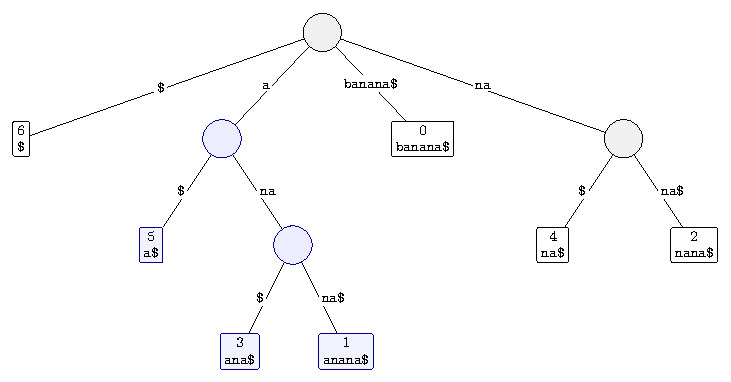
\includegraphics[width=0.82\textwidth]{images/suffix-array/banana-suffix-tree.pdf}
    \caption{\texten{Suffix tree} compatto di \texttt{banana\$}}
    \label{fig:banana_suffix_tree}
\end{figure}

\autoref{fig:banana_suffix_tree} mostra lo stesso esempio come albero dei suffissi. Ogni foglia contiene la posizione iniziale del suffisso corrispondente; leggendo le foglie da sinistra a destra si ritrova:
\[
    6,5,3,1,0,4,2,
\]
cioè il \texten{suffix array}. Il sottoalbero evidenziato sotto l'arco \texttt{a} contiene proprio le foglie $5,3,1$, che corrispondono ai suffissi \texttt{a\$}, \texttt{ana\$} e \texttt{anana\$}. Questa è la versione ad albero dell'intervallo $SA[1,3]$ nella rappresentazione tramite \texten{suffix array}.

\subsubsection{BWT da suffix array}
Una volta costruito il \texten{suffix array} di $T=s\texttt{\$}$, la BWT si ottiene in modo diretto. Se $SA[r]=i$, allora la riga di rango $r$ corrisponde alla rotazione che inizia in $i$, oppure, equivalentemente, al suffisso che parte da $i$. Il carattere della colonna $L$ è il carattere che precede quel suffisso nel testo:
\begin{equation}\label{eq:bwt_from_suffix_array}
    L[r]=
    \begin{cases}
        T[SA[r]-1]=T[i-1], & \text{se } i>0, \\
        \texttt{\$},       & \text{se } i=0.
    \end{cases}
\end{equation}
Il secondo caso gestisce la rotazione ciclica: se il suffisso parte dall'inizio del testo, il carattere precedente è il simbolo finale \texttt{\$}, cioè $T[n-1]$.

\paragraph{Esempio: \texttt{abaaba\$}.}
Per:
\[
    T=\texttt{abaaba\$},
\]
il \texten{suffix array} è:
\[
    SA=(6,5,2,3,0,4,1).
\]
Per costruire la BWT non serve scrivere tutta la matrice delle rotazioni: basta prendere, per ogni suffisso ordinato, il carattere immediatamente precedente nel testo.

\begin{table}[H]
    \centering
    \begin{tabular}{c|c|c|c}
        \textbf{rango $r$} & \textbf{$SA[r]$} & \textbf{suffisso} & \textbf{$L[r]$} \\ \hline
        $0$                & $6$              & \texttt{\$}       & \texttt{a}      \\
        $1$                & $5$              & \texttt{a\$}      & \texttt{b}      \\
        $2$                & $2$              & \texttt{aaba\$}   & \texttt{b}      \\
        $3$                & $3$              & \texttt{aba\$}    & \texttt{a}      \\
        $4$                & $0$              & \texttt{abaaba\$} & \texttt{\$}     \\
        $5$                & $4$              & \texttt{ba\$}     & \texttt{a}      \\
        $6$                & $1$              & \texttt{baaba\$}  & \texttt{a}
    \end{tabular}
    \caption{Calcolo della BWT di \texttt{abaaba\$} dal \texten{suffix array}}
    \label{tab:bwt_from_suffix_array_abaaba}
\end{table}

Leggendo l'ultima colonna della tabella:
\[
    \operatorname{BWT}(T)=\texttt{abba\$aa}.
\]
Il vantaggio è che non abbiamo dovuto ordinare esplicitamente tutte le rotazioni: è sufficiente costruire il \texten{suffix array} e poi leggere un carattere per ogni posizione dell'array.

\subsection{Algoritmo DC3 per costruire il suffix array}
Il tempo di calcolo della BWT dipende dal tempo necessario a costruire il \texten{suffix array}. Se il \texten{suffix array} si costruisce in tempo lineare, allora anche la fase BWT, una volta noto l'array, richiede solo tempo lineare.

Per la costruzione di SA esistono e sono stati creati diversi algoritmi, tra cui:
\begin{itemize}
    \item \textbf{DC3}, basato su \texten{difference cover sampling};
    \item \textbf{SA-IS}, basato su \texten{induced sorting};
    \item approcci non ricorsivi più recenti, come quello di Baier;
\end{itemize}
qui ci concentriamo su DC3.

\subsubsection{Schema ricorsivo generale}
L'idea è ordinare prima una parte dei suffissi, codificare quell'ordine in una stringa più corta e poi usare tale informazione per ordinare tutti i suffissi del testo.

Gli algoritmi come DC3 e SA-IS usano una strategia di campionamento. Supponiamo che l'alfabeto sia rappresentato da interi positivi e che:
\[
    T[n]=0
\]
sia un simbolo di fine stringa minore di tutti gli altri.

Lo schema generale è:
\begin{enumerate}
    \item scegliere un sottoinsieme di posizioni $C\subseteq [0,n]$;
    \item ordinare i suffissi che partono da posizioni in $C$;
    \item usare l'ordine dei suffissi campionati per ordinare tutti gli altri suffissi;
    \item fondere le liste ordinate in un unico \texten{suffix array}.
\end{enumerate}

Il punto cruciale è che $C$ deve essere abbastanza piccolo da permettere una chiamata ricorsiva su un input più corto, ma abbastanza informativo da permettere confronti in tempo costante durante la fusione. Se:
\[
    |C|\leq \alpha n
    \qquad
    \text{con } \alpha<1,
\]
e tutte le fasi non ricorsive costano $O(n)$, la complessità soddisfa:
\begin{equation}\label{eq:recursive_sa_recurrence}
    T(n)=T(\alpha n)+O(n),
\end{equation}
e quindi:
\[
    T(n)=O(n).
\]

\subsubsection{I tre passi di DC3}
DC3 costruisce il \texten{suffix array} senza ordinare direttamente tutti i suffissi del testo. L'idea è dividere le posizioni in due gruppi: prima si ordinano circa due terzi dei suffissi, poi si usa l'ordine ottenuto per ordinare il terzo rimasto e per fondere tutto.

La divisione è fatta usando le classi di resto modulo $3$:
\[
    P_{1,2}=\{i\mid i\bmod 3=1 \text{ oppure } i\bmod 3=2\},
    \qquad
    P_0=\{i\mid i\bmod 3=0\}.
\]
Il campione $P_{1,2}$ contiene circa $\frac{2}{3}$ delle $n$ posizioni; il resto $P_0$ ne contiene circa $\frac{1}{3}$. Quando servono caratteri oltre la fine del testo, si usa il simbolo finale minimo come \texten{padding}: serve solo a completare le ultime triplette, non ad aggiungere nuovi suffissi da ordinare.

\begin{algorithm}[htpb]
    \caption{Schema dell'algoritmo DC3}
    \begin{algorithmic}[1]
        \Require testo $T[0,n)$ con simbolo finale minimo
        \Ensure \texten{suffix array} $SA$ di $T$
        \Statex \textbf{Passo 1: suffissi campionati}
        \State dividi le posizioni in $P_{1,2}$ e $P_0$
        \State costruisci le triplette che iniziano nelle posizioni di $P_{1,2}$
        \State ordina le triplette e assegna un rango a ogni tripletta distinta
        \State concatena i ranghi ottenendo la stringa ridotta $T^{1,2}$
        \State calcola il \texten{suffix array} $SA'$ di $T^{1,2}$, ricorsivamente se i ranghi non sono tutti distinti
        \State traduci le posizioni di $SA'$ nelle corrispondenti posizioni del testo, ottenendo $SA^{1,2}$
        \State costruisci l'array inverso $\operatorname{pos}$ dei ranghi dei suffissi in $SA^{1,2}$
        \Statex \textbf{Passo 2: suffissi non campionati}
        \State per ogni $i\in P_0$, rappresenta $T[i,n)$ con $\langle T[i],\operatorname{pos}(i+1)\rangle$
        \State ordina queste coppie con \texten{radix sort}, ottenendo $SA^0$
        \Statex \textbf{Passo 3: fusione}
        \State fondi $SA^{1,2}$ e $SA^0$ usando confronti in tempo costante basati sui ranghi già calcolati
        \State \Return $SA$
    \end{algorithmic}
\end{algorithm}

\begin{figure}[H]
    \centering
    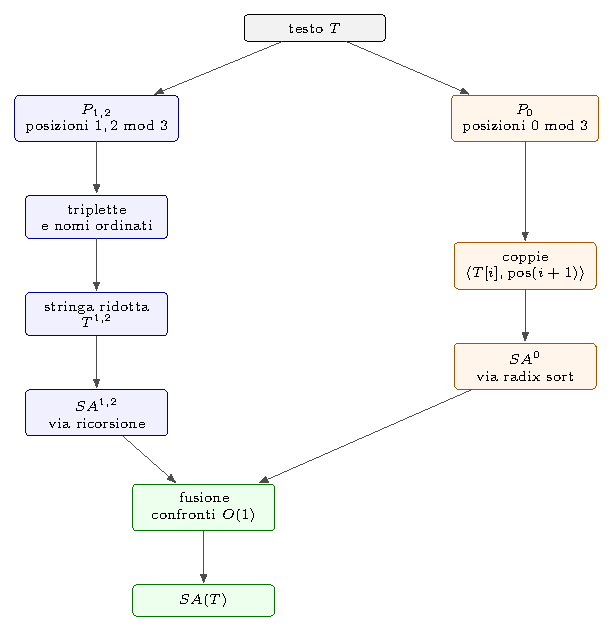
\includegraphics[width=0.72\textwidth]{images/suffix-array/dc3-overview.pdf}
    \caption{Schema ricorsivo dei tre passi principali di DC3}
    \label{fig:dc3_overview}
\end{figure}

La \autoref{fig:dc3_overview} riassume il flusso logico. La parte blu è quella ricorsiva: dai suffissi campionati si costruisce una stringa ridotta e se ne calcola il \texten{suffix array}. La parte arancione ordina i suffissi non campionati usando i ranghi già noti. La parte verde fonde le due liste ordinate. Il punto importante è che, dopo il primo passo, non conosciamo solo una lista ordinata: conosciamo anche il rango dei suffissi campionati, e questi ranghi diventano abbreviazioni usabili nei passi successivi.

\paragraph{Passo 1: ordinare i suffissi in $P_{1,2}$.}
Si vogliono ordinare solo i suffissi che partono nelle posizioni di $P_{1,2}$. Per farlo, DC3 costruisce una stringa ridotta $T^{1,2}$ lunga circa $\frac{2}{3}n$: ogni simbolo di questa nuova stringa è il rango lessicografico di una tripletta di caratteri del testo originale.

Le triplette si ottengono guardando due sequenze:
\[
    T[1,\cdot]
    =
    [T[1],T[2],T[3]]
    [T[4],T[5],T[6]]
    [T[7],T[8],T[9]]
    \cdots
\]
e:
\[
    T[2,\cdot]
    =
    [T[2],T[3],T[4]]
    [T[5],T[6],T[7]]
    [T[8],T[9],T[10]]
    \cdots
\]
La prima sequenza descrive le posizioni dove il primo indice della tripletta è congruente a $1$ modulo $3$, la seconda quelle congruenti a $2$ modulo $3$. Concatenando i ranghi delle triplette di $T[1,\cdot]$ e poi quelli delle triplette di $T[2,\cdot]$ si ottiene $T^{1,2}$.

Perché questo è utile? Un suffisso che parte in $P_{1,2}$ può essere letto come una sequenza di triplette: confrontare due di questi suffissi equivale quindi a confrontare due suffissi della stringa di ranghi $T^{1,2}$. Se due triplette sono diverse, il loro rango decide subito; se sono uguali, si passa alla tripletta successiva, cioè al simbolo successivo di $T^{1,2}$.

Per esempio, con:
\[
    T=\texttt{mississippi\$},
\]
le posizioni sono:
\[
    P_{1,2}=\{1,2,4,5,7,8,10,11\},
    \qquad
    P_0=\{0,3,6,9\}.
\]
Si considerano:
\[
    T[1,\cdot]
    =
    [\texttt{i s s}]
    [\texttt{i s s}]
    [\texttt{i p p}]
    [\texttt{i \$ \$}],
\]
e:
\[
    T[2,\cdot]
    =
    [\texttt{s s i}]
    [\texttt{s s i}]
    [\texttt{p p i}]
    [\texttt{\$ \$ \$}].
\]
Ora si applica il \textbf{\texten{lexicographic naming}} delle triplette. Il rango non è ancora il rango del suffisso intero: è solo un nuovo nome numerico assegnato alla tripletta in base alla sua posizione nell'ordine lessicografico. Si ordinano quindi le triplette distinte:
\[
    [\texttt{\$ \$ \$}]<[\texttt{i \$ \$}]<[\texttt{i p p}]<[\texttt{i s s}]<[\texttt{p p i}]<[\texttt{s s i}],
\]
e si assegna rango $0$ alla più piccola, rango $1$ alla successiva, e così via:

\[
    \begin{array}{c|cccccc}
        \text{tripletta} & \texttt{\$ \$ \$} & \texttt{i \$ \$} & \texttt{i p p} & \texttt{i s s} & \texttt{p p i} & \texttt{s s i} \\ \hline
        \text{rango}     & 0                 & 1                & 2              & 3              & 4              & 5
    \end{array}
\]

Le occorrenze uguali ricevono lo stesso rango. Tornando allora all'ordine in cui le triplette erano state concatenate, si ottiene la seguente sostituzione:

\begin{center}
    \begin{tabular}{c|cccccccc}
        \textbf{posizione in $T$} & $1$          & $4$          & $7$          & $10$           & $2$          & $5$          & $8$          & $11$            \\ \hline
        \textbf{tripletta}        & \texttt{iss} & \texttt{iss} & \texttt{ipp} & \texttt{i\$\$} & \texttt{ssi} & \texttt{ssi} & \texttt{ppi} & \texttt{\$\$\$} \\
        \textbf{rango}            & $3$          & $3$          & $2$          & $1$            & $5$          & $5$          & $4$          & $0$
    \end{tabular}
\end{center}

La stringa ridotta è quindi:
\[
    T^{1,2}=(3,3,2,1,5,5,4,0).
\]
Se tutti i simboli di $T^{1,2}$ fossero distinti, i suffissi campionati sarebbero già ordinabili guardando il primo rango. Qui invece compaiono ripetizioni, per esempio i ranghi $3$ e $5$, quindi bisogna ordinare i suffissi di $T^{1,2}$ ricorsivamente. Per costruire il \texten{suffix array}, trattiamo $T^{1,2}$ come una normale stringa di interi e ordiniamo lessicograficamente i suoi suffissi. Nella tabella seguente il rango è la posizione del suffisso nell'ordine lessicografico finale:

\begin{center}
    \begin{tabular}{c|c|l}
        \textbf{rango} & \textbf{posizione in $T^{1,2}$} & \textbf{suffisso} \\ \hline
        $0$            & $7$                             & $0$               \\
        $1$            & $3$                             & $1,5,5,4,0$       \\
        $2$            & $2$                             & $2,1,5,5,4,0$     \\
        $3$            & $1$                             & $3,2,1,5,5,4,0$   \\
        $4$            & $0$                             & $3,3,2,1,5,5,4,0$ \\
        $5$            & $6$                             & $4,0$             \\
        $6$            & $5$                             & $5,4,0$           \\
        $7$            & $4$                             & $5,5,4,0$
    \end{tabular}
\end{center}

Le posizioni lette nella seconda colonna formano quindi il \texten{suffix array}. Quindi otteniamo:
\[
    SA(T^{1,2})=(7,3,2,1,0,6,5,4).
\]
Questo array però è espresso in posizioni della stringa ridotta. Per tornare al testo originale si usa il modo in cui $T^{1,2}$ è stato costruito: le prime quattro posizioni corrispondono ai suffissi che partono da $1,4,7,10$, mentre le ultime quattro corrispondono ai suffissi che partono da $2,5,8,11$:
\[
    \begin{array}{c|cccccccc}
        \text{posizione in }T^{1,2} & 0 & 1 & 2 & 3  & 4 & 5 & 6 & 7  \\ \hline
        \text{posizione in }T       & 1 & 4 & 7 & 10 & 2 & 5 & 8 & 11
    \end{array}
\]
Applicando questa conversione a $SA(T^{1,2})$:
\[
    SA^{1,2}=(11,10,7,4,1,8,5,2).
\]

\paragraph{Passo 2: ordinare i suffissi in $P_0$.}
Ora mancano i suffissi che partono nelle posizioni di $P_0$. Se $i\in P_0$, allora $i+1\in P_{1,2}$, quindi il suffisso $T[i+1,n)$ è già stato ordinato nel passo precedente. Per questo si può decomporre:
\[
    T[i,n)=T[i]\;T[i+1,n)
\]
e rappresentare $T[i,n)$ con la coppia:
\[
    \langle T[i],\operatorname{pos}(i+1)\rangle,
\]
dove $\operatorname{pos}(i+1)$ è il rango del suffisso $T[i+1,n)$ dentro $SA^{1,2}$. L'array $\operatorname{pos}$ è quindi l'inverso di $SA^{1,2}$: se un suffisso compare in posizione $r$ dentro $SA^{1,2}$, il suo rango è $r$. Per le posizioni oltre la fine del testo si usa rango $0$, coerentemente con il \texten{padding}.

Questa coppia non contiene tutto il suffisso, ma contiene esattamente l'informazione necessaria per confrontare due suffissi che partono in $P_0$. Se due suffissi $T[i,n)$ e $T[h,n)$ hanno primo carattere diverso, decide il confronto tra $T[i]$ e $T[h]$; se invece hanno lo stesso primo carattere, resta da confrontare $T[i+1,n)$ con $T[h+1,n)$. Poiché $i+1$ e $h+1$ appartengono a $P_{1,2}$, il loro ordine è già noto attraverso $\operatorname{pos}$. Per questo ordinare le coppie $\langle T[i],\operatorname{pos}(i+1)\rangle$ equivale a ordinare i suffissi di $P_0$, ma costa solo tempo lineare con \texten{radix sort}.

Nel caso:
\[
    T=\texttt{mississippi\$},
    \qquad
    SA^{1,2}=(11,10,7,4,1,8,5,2),
\]
si costruisce prima:
\[
    \begin{array}{c|cccccccc}
        k                     & 11 & 10 & 7 & 4 & 1 & 8 & 5 & 2 \\ \hline
        \operatorname{pos}(k) & 0  & 1  & 2 & 3 & 4 & 5 & 6 & 7
    \end{array}
\]
e poi, per $P_0=\{0,3,6,9\}$, le seguenti coppie:

\begin{center}
    \begin{tabular}{c|c|c}
        \textbf{posizione $i$} & \textbf{suffisso $T[i,n)$} & \textbf{coppia}               \\ \hline
        $0$                    & \texttt{mississippi\$}     & $\langle \texttt{m},4\rangle$ \\
        $3$                    & \texttt{sissippi\$}        & $\langle \texttt{s},3\rangle$ \\
        $6$                    & \texttt{sippi\$}           & $\langle \texttt{s},2\rangle$ \\
        $9$                    & \texttt{pi\$}              & $\langle \texttt{p},1\rangle$
    \end{tabular}
\end{center}

Ordinando queste coppie con \texten{radix sort}:
\[
    SA^0=(0,9,6,3).
\]

\paragraph{Passo 3: fusione.}
Resta da fondere $SA^{1,2}$ e $SA^0$. Questa è una fusione tra due liste già ordinate, come nel \texten{merge sort}; l'unica difficoltà è decidere quale dei due suffissi in testa alle liste venga prima in ordine lessicografico. DC3 evita confronti carattere per carattere usando ancora i ranghi già calcolati.

La scelta delle classi $1$ e $2$ modulo $3$ serve proprio a questo: se un suffisso parte in $P_0$, dopo aver saltato uno o due caratteri si arriva sempre a una posizione campionata, quindi a un suffisso di rango già noto. Sia $i\in P_0$ e sia $j\in P_{1,2}$. Ci sono due casi\footnote{Il motivo della distinzione è modulare. Se $j\bmod 3=1$, allora $j+1\bmod 3=2$, quindi dopo un carattere si arriva ancora in $P_{1,2}$ e il rango è noto. Se invece $j\bmod 3=2$, allora $j+1\bmod 3=0$, quindi dopo un solo carattere si finirebbe in $P_0$, dove il rango non è noto; bisogna avanzare di un altro carattere, arrivando a $j+2\bmod 3=1$.}:
\begin{itemize}
    \item se $j\bmod 3=1$, allora si confrontano le coppie:
          \[
              \langle T[i],\operatorname{pos}(i+1)\rangle
              \quad
              \text{e}
              \quad
              \langle T[j],\operatorname{pos}(j+1)\rangle;
          \]
    \item se $j\bmod 3=2$, allora si confrontano le triplette:
          \[
              \langle T[i],T[i+1],\operatorname{pos}(i+2)\rangle
              \quad
              \text{e}
              \quad
              \langle T[j],T[j+1],\operatorname{pos}(j+2)\rangle.
          \]
\end{itemize}
In entrambi i casi il confronto costa $O(1)$, perché dopo uno o due caratteri si arriva a suffissi il cui rango è già noto in $SA^{1,2}$.

Per l'esempio:
\[
    T=\texttt{mississippi\$},
\]
partendo da:
\[
    SA^{1,2}=(11,10,7,4,1,8,5,2),
    \qquad
    SA^0=(0,9,6,3),
\]
conviene tenere esplicite le chiavi che saranno usate durante la fusione. Per gli elementi di $SA^0$ si preparano sia la coppia sia la tripletta, perché il tipo di confronto dipende dall'elemento di $SA^{1,2}$ con cui verranno confrontati:

\begin{table}[htpb]
    \centering
    \small
    \begin{minipage}{0.44\textwidth}
        \centering
        \[
            \begin{array}{c|c|c}
                \multicolumn{3}{c}{SA^0=(0,9,6,3)}                                       \\
                i & \text{coppia}               & \text{tripletta}                       \\ \hline
                0 & \langle \texttt{m},4\rangle & \langle \texttt{m},\texttt{i},7\rangle \\
                9 & \langle \texttt{p},1\rangle & \langle \texttt{p},\texttt{i},0\rangle \\
                6 & \langle \texttt{s},2\rangle & \langle \texttt{s},\texttt{i},5\rangle \\
                3 & \langle \texttt{s},3\rangle & \langle \texttt{s},\texttt{i},6\rangle
            \end{array}
        \]
    \end{minipage}
    \hfill
    \begin{minipage}{0.52\textwidth}
        \centering
        \[
            \begin{array}{c|c|c}
                \multicolumn{3}{c}{SA^{1,2}=(11,10,7,4,1,8,5,2)}                 \\
                j  & \text{caso}      & \text{chiave usata}                      \\ \hline
                11 & \text{tripletta} & \langle \texttt{\$},\texttt{\$},0\rangle \\
                10 & \text{coppia}    & \langle \texttt{i},0\rangle              \\
                7  & \text{coppia}    & \langle \texttt{i},5\rangle              \\
                4  & \text{coppia}    & \langle \texttt{i},6\rangle              \\
                1  & \text{coppia}    & \langle \texttt{i},7\rangle              \\
                8  & \text{tripletta} & \langle \texttt{p},\texttt{p},1\rangle   \\
                5  & \text{tripletta} & \langle \texttt{s},\texttt{s},2\rangle   \\
                2  & \text{tripletta} & \langle \texttt{s},\texttt{s},3\rangle
            \end{array}
        \]
    \end{minipage}
    \caption{Chiavi locali usate nella fusione tra $SA^0$ e $SA^{1,2}$ per $T=\texttt{mississippi\$}$.}
    \label{tab:dc3_merge_keys_mississippi}
\end{table}

La colonna ``caso'' di $SA^{1,2}$ indica quale chiave confrontare: se è una coppia si usa anche la coppia dell'elemento di $SA^0$, mentre se è una tripletta si usa la tripletta. Per esempio, confrontando $i=0$ con $j=1$ si confrontano $\langle\texttt{m},4\rangle$ e $\langle\texttt{i},7\rangle$; confrontando $i=0$ con $j=8$ si confrontano invece $\langle\texttt{m},\texttt{i},7\rangle$ e $\langle\texttt{p},\texttt{p},1\rangle$.

La fusione produce:
\[
    SA=(11,10,7,4,1,0,9,8,6,3,5,2).
\]

\subsubsection{Esercizio guidato: \texttt{yabbadabbado\$}}
Applichiamo DC3 alla stringa:
\[
    T=\texttt{yabbadabbado\$}.
\]
Il \texten{suffix array} finale atteso è:
\[
    SA=(12,1,6,4,9,3,8,2,7,5,10,11,0).
\]

Nel primo passo si prendono le posizioni congruenti a $1$ e $2$ modulo $3$:
\[
    \{1,4,7,10,2,5,8,11\}.
\]
Le triplette sono:
\[
    [\texttt{abb}]
    [\texttt{ada}]
    [\texttt{bba}]
    [\texttt{do\$}]
    [\texttt{bba}]
    [\texttt{dab}]
    [\texttt{bad}]
    [\texttt{o\$\$}].
\]
Ordinandole e sostituendole con i rispettivi ranghi, si ottiene:
\[
    u'=(1,2,4,6,4,5,3,7),
\]
a cui si aggiunge un simbolo di fine stringa. Da questa stringa ridotta si ottiene:
\[
    SA(u')=(0,1,6,4,2,5,3,7).
\]
Da qui si ricava:
\[
    SA^{1,2}=(1,4,8,2,7,5,10,11).
\]
Per le posizioni in $P_0$ si ottiene:
\[
    SA^0=(12,6,9,3,0),
\]
perché:
\[
    (\texttt{\$},0)<(\texttt{a},5)<(\texttt{a},7)<(\texttt{b},2)<(\texttt{y},1).
\]
La fusione delle due liste dà il \texten{suffix array} finale indicato sopra.

\subsubsection{Complessità e Master Theorem}
La complessità di DC3 è modellata dalla ricorrenza:
\begin{equation}\label{eq:dc3_recurrence}
    T(n)=T\left(\frac{2}{3}n\right)+O(n).
\end{equation}
La chiamata ricorsiva lavora infatti sulla stringa ridotta associata a $P_{1,2}$, lunga circa $\frac{2}{3}n$, mentre le altre fasi costano tempo lineare grazie a \texten{radix sort} e alla fusione con confronti in tempo costante. La soluzione della ricorrenza è:
\[
    T(n)=O(n).
\]

Richiamiamo anche la forma classica del Master Theorem. Se:
\[
    T(n)=aT(n/b)+f(n),
    \qquad
    T(1)=c,
\]
con $a\geq 1$, $b>1$ e $f(n)\in \Theta(n^d)$, allora:
\[
    T(n)=
    \begin{cases}
        \Theta(n^d),          & \text{se } a<b^d, \\
        \Theta(n^d\log n),    & \text{se } a=b^d, \\
        \Theta(n^{\log_b a}), & \text{se } a>b^d.
    \end{cases}
\]
Per esempio:
\[
    T(n)=T(n/2)+\frac{1}{2}n^2+n
\]
ha $a=1$, $b=2$, $d=2$ e $1<2^2$, quindi:
\[
    T(n)\in\Theta(n^2).
\]
Nel caso DC3, invece, la ricorrenza non ha due sottoproblemi: c'è una sola chiamata ricorsiva su una frazione stretta dell'input, più lavoro lineare. La somma dei costi sui livelli della ricorsione è:
\[
    n+\frac{2}{3}n+\left(\frac{2}{3}\right)^2n+\cdots=O(n).
\]

\subsubsection{Difference cover}
Il campionamento di DC3 è un caso particolare di \textbf{difference cover}. Un difference cover $D_q$ modulo $q$ è un sottoinsieme di $[0,q)$ tale che ogni valore modulo $q$ può essere espresso come differenza di due elementi di $D_q$:
\begin{equation}\label{eq:difference_cover_definition}
    [0,q)
    =
    \{i-j \bmod q \mid i,j\in D_q\}.
\end{equation}

Per esempio:
\[
    D_7=\{1,2,4\}
\]
è un difference cover modulo $7$, perché:
\[
    \begin{array}{rclcrcl}
        1-1 & \equiv & 0 & \pmod 7, & 1-4 & \equiv & 4 \pmod 7, \\
        2-1 & \equiv & 1 & \pmod 7, & 2-4 & \equiv & 5 \pmod 7, \\
        4-2 & \equiv & 2 & \pmod 7, & 1-2 & \equiv & 6 \pmod 7, \\
        4-1 & \equiv & 3 & \pmod 7. &
    \end{array}
\]
DC3 usa il più semplice difference cover non banale:
\[
    D_3=\{1,2\}.
\]
Infatti, modulo $3$, le differenze tra elementi di $D_3$ producono tutte le classi:
\[
    \begin{aligned}
        1-1 & \equiv 0 \pmod 3, \\
        2-1 & \equiv 1 \pmod 3, \\
        1-2 & \equiv 2 \pmod 3.
    \end{aligned}
\]
La generalizzazione dell'algoritmo seleziona posizioni congruenti agli elementi di un difference cover modulo $q$, forma $q$-uple invece di triplette, costruisce una stringa ridotta $R$, la ordina ricorsivamente e poi fonde i suffissi. La complessità diventa $O(qn)$; questa generalizzazione è utile soprattutto per implementazioni più attente allo spazio.

\subsection{Proprietà combinatorie della BWT}
La BWT ha anche proprietà combinatorie indipendenti dall'uso come compressore. Due parole $x$ e $y$ su un alfabeto finito $\Sigma$ si dicono \textbf{coniugate} se una è una rotazione ciclica dell'altra.

Se non si considera l'indice $I$ nella BWT, allora valgono le seguenti proprietà:
\begin{itemize}
    \item due testi $x$ e $y$ sono coniugati se e solo se:
          \[
              \operatorname{BWT}(x)=\operatorname{BWT}(y);
          \]
    \item dati due testi $u$ e $v$, $u$ è coniugato di $v^d$ se e solo se, ponendo:
          \[
              \operatorname{BWT}(v)=a_0a_1\cdots a_{n-1},
          \]
          si ha:
          \[
              \operatorname{BWT}(u)=a_0^d a_1^d\cdots a_{n-1}^d.
          \]
\end{itemize}

Queste proprietà chiariscono anche un punto pratico: i testi più favorevoli a una compressione BWT-based sono quelli la cui trasformata contiene poche run di lettere uguali. In altre parole, la BWT è particolarmente utile quando l'ordinamento dei contesti produce \textbf{clustering}.

\paragraph{Perfect clustering nel caso binario.}
Nel caso di alfabeti binari, è stato dimostrato che la BWT produce un clustering perfetto, cioè una stringa del tipo:
\[
    1^p0^q,
\]
con $p$ e $q$ coprimi, se e solo se il testo è una rotazione ciclica di una parola Sturmiana standard. Le parole di Fibonacci sono un caso particolare di parole Sturmiane standard. Questo collegamento è naturale perché le parole Sturmiane codificano linee digitali, cioè traiettorie discrete che approssimano rette nel piano.

Per alfabeti più grandi, il problema è stato risolto nel 2013 da Ferenczi e Zamboni tramite la codifica di particolari traiettorie nel piano. Per gli scopi della compressione, la morale è più semplice: la BWT è efficace quando trasforma la struttura contestuale del testo in poche run visibili nella colonna $L$.

\subsection{Pattern matching e FM-index}
Finora la BWT è stata vista soprattutto come trasformazione utile alla compressione. La stessa struttura, però, permette anche di costruire indici compressi: invece di decomprimere un testo e poi cercare un pattern, si conserva una rappresentazione compressa che supporta direttamente operazioni di ricerca. L'obiettivo di questa sezione è quello di spiegare come funziona la ricerca di pattern nel testo e come un indice compresso basato sulla BWT, chiamato \textbf{\texten{FM-index}}, permette di eseguire questa ricerca in modo efficiente.

Dato un testo $T[1..n]$ e un pattern $P[1..p]$, vogliamo:
\begin{itemize}
    \item \textbf{\texten{count}}: contare quante volte $P$ compare in $T$;
    \item \textbf{\texten{locate}}: restituire le posizioni di tutte le occorrenze.
\end{itemize}

Un algoritmo classico come Knuth-Morris-Pratt cerca $P$ in tempo $O(n+p)$ senza costruire un indice. Se però il testo o la collezione sono noti in anticipo, conviene pagare una fase di preprocessing e costruire una struttura dati che renda molte ricerche successive più veloci.

\subsubsection{Ricerca tramite suffix array}
Il \texten{suffix array} è un indice naturale per il \texten{pattern matching}: se $P$ compare in $T$ alla posizione $i$, allora $P$ è prefisso del suffisso $T[i..n]$. Poiché il \texten{suffix array} ordina lessicograficamente tutti i suffissi, le occorrenze di $P$ formano un intervallo contiguo dell'array.

Per cercare $P$ si può quindi fare una ricerca binaria tra i suffissi ordinati. A ogni confronto si confrontano al più $p$ caratteri, quindi il tempo è:
\[
    O(p\log n).
\]
Con informazioni ausiliarie, per esempio basate sugli \texten{LCP}, il tempo può essere ridotto a:
\[
    O(p+\log n).
\]

Il costo in spazio è però alto. Un \texten{suffix array} contiene $n$ interi nell'intervallo $[1,n]$, quindi richiede idealmente:
\[
    n\log n
    \quad
    \text{bit}.
\]
Nelle implementazioni comuni, se ogni posizione occupa $4$ \texten{byte}, un testo da $100$ \texten{MB} può richiedere circa $400$ \texten{MB} solo per il \texten{suffix array}. Il punto degli indici compressi è proprio combinare due esigenze che sembrano in tensione: \textbf{poco spazio} e \textbf{ricerca veloce}.

Una compressione generica del testo non basta a risolvere questo problema. Strumenti come gzip o bzip2 possono ridurre molto lo spazio occupato, ma se il risultato è soltanto un file compresso, per cercare un pattern bisogna in genere decomprimere almeno una parte consistente del testo. Un \textbf{indice compresso} ha invece un obiettivo più ambizioso: conservare una rappresentazione vicina alla dimensione compressa del testo e supportare direttamente le operazioni di ricerca.

\subsubsection{Backward search sulla BWT}
L'idea dell'\textbf{\texten{FM-index}}, introdotto da Ferragina e Manzini, è usare la BWT come se fosse un \texten{suffix array} compresso. Le righe della matrice BWT sono le rotazioni ordinate del testo, e quindi sono strettamente legate ai suffissi ordinati. Per contare le occorrenze di $P$ non serve ricostruire $T$: basta lavorare sulla colonna $L=\operatorname{BWT}(T)$ e su due strutture ausiliarie.

Usiamo indici da $1$ a $n$ e indichiamo con:
\begin{itemize}
    \item $C(c)$ il numero di caratteri di $T$ strettamente minori di $c$;
    \item $\operatorname{Occ}(c,q)$ il numero di occorrenze di $c$ nel prefisso $L[1..q]$, con $\operatorname{Occ}(c,0)=0$.
\end{itemize}

La formula LF-mapping, nella convenzione a indici da $1$, diventa:
\[
    \operatorname{LF}(i)
    =
    C(L[i])+\operatorname{Occ}(L[i],i).
\]
Più precisamente, se la riga $i$ rappresenta il suffisso che inizia in posizione $k$, allora $\operatorname{LF}(i)$ rappresenta il suffisso che inizia in posizione $k-1$.\footnote{Quando $k=1$, il passo attraversa il simbolo di fine testo e si interpreta il testo in modo circolare. L'idea è che $L[i]$ è proprio il carattere che precede, nel testo originale, il suffisso rappresentato dalla riga $i$; la LF-mapping sposta quindi la riga verso il suffisso ottenuto aggiungendo quel carattere a sinistra.}

Lo schema mentale è il seguente. Se una riga inizia con un certo testo $Q$ e nella sua colonna $L$ compare il carattere $c$, allora LF porta alla riga che inizia con $cQ$:
\[
    \boxed{
        \begin{array}{c}
            \text{riga } i                    \\
            \text{suffisso rappresentato: } Q \\
            L[i]=c
        \end{array}
    }
    \quad
    \xrightarrow{\operatorname{LF}}
    \quad
    \boxed{
        \begin{array}{c}
            \text{riga } \operatorname{LF}(i) \\
            \text{suffisso rappresentato: } cQ
        \end{array}
    }
\]
Per esempio, se la riga corrente rappresenta un suffisso che inizia con \texttt{i} e in $L$ compare \texttt{s}, allora LF porta alla riga del suffisso che inizia con \texttt{si}.

La \textbf{\texten{backward search}} mantiene l'intervallo di righe che hanno come prefisso il suffisso già letto del pattern. All'inizio l'intervallo è tutto $[1,n]$. Se il prossimo carattere da aggiungere a sinistra è $c=P[j]$, l'intervallo si aggiorna con:
\begin{align}
    \textit{First}' & =
    C(c)+\operatorname{Occ}(c,\textit{First}-1)+1,
    \label{eq:fm_backward_first} \\
    \textit{Last}'  & =
    C(c)+\operatorname{Occ}(c,\textit{Last}).
    \label{eq:fm_backward_last}
\end{align}
Se dopo un aggiornamento $\textit{First}>\textit{Last}$, il pattern non compare. Altrimenti, dopo aver processato tutti i caratteri da destra verso sinistra, il numero di occorrenze è:
\[
    \textit{Last}-\textit{First}+1.
\]

\begin{algorithm}[htpb]
    \caption{\texten{Backward search}}
    \begin{algorithmic}[1]
        \Require pattern $P[1..p]$, colonna BWT $L$, strutture $C$ e $\operatorname{Occ}$
        \Ensure intervallo delle righe prefissate da $P$
        \State $\textit{First}\gets 1$
        \State $\textit{Last}\gets n$
        \For{$j=p$ \textbf{downto} $1$}
        \State $c\gets P[j]$
        \State $\textit{First}\gets C(c)+\operatorname{Occ}(c,\textit{First}-1)+1$
        \State $\textit{Last}\gets C(c)+\operatorname{Occ}(c,\textit{Last})$
        \If{$\textit{First}>\textit{Last}$}
        \State \Return intervallo vuoto
        \EndIf
        \EndFor
        \State \Return $[\textit{First},\textit{Last}]$
    \end{algorithmic}
\end{algorithm}

L'aspetto importante è che il numero di iterazioni è $p$: una per carattere del pattern. Se $\operatorname{Occ}$ è disponibile in tempo $O(1)$, il conteggio richiede tempo $O(p)$.

Un modo banale per ottenere questa prestazione sarebbe memorizzare una tabella completa:
\[
    \operatorname{OCC}[c][q]
    =
    \operatorname{Occ}(c,q),
    \qquad
    c\in\Sigma,\ 1\leq q\leq n.
\]
In questo caso la \texten{backward search} sarebbe effettivamente veloce, ma la tabella richiederebbe:
\[
    O(|\Sigma|\,n\log n)
\]
bit. Per alfabeti costanti questo è ancora $O(n\log n)$ bit, cioè dello stesso ordine di grandezza di un \texten{suffix array} esplicito. Il punto tecnico dell'FM-index è quindi implementare $\operatorname{Occ}$ in tempo costante senza pagare una tabella completa.

\paragraph{Esempio intuitivo.}
Nel testo \texttt{mississippi\#}, tutti i suffissi che iniziano con \texttt{i} occupano un intervallo contiguo della matrice ordinata. Per cercare \texttt{si}, la ricerca parte dall'ultimo carattere \texttt{i}: l'intervallo corrente contiene quindi le righe che iniziano con il suffisso già letto, cioè \texttt{i}. Aggiungere a sinistra il carattere \texttt{s} significa chiedersi quali di quelle occorrenze di \texttt{i} erano precedute da una \texttt{s} nel testo originale.

Questa informazione è contenuta nella colonna $L$: se una riga $r$ dell'intervallo corrente ha $L[r]=\texttt{s}$, allora il suffisso rappresentato da quella riga è preceduto da \texttt{s}, quindi corrisponde a un'occorrenza di \texttt{si}. Tuttavia l'algoritmo non scorre davvero tutte le righe dell'intervallo per filtrare quelle con $L=\texttt{s}$. Usa invece $\operatorname{Occ}$ per sapere quali occorrenze di \texttt{s} cadono dentro l'intervallo corrente.

In generale, se l'intervallo corrente è $[\textit{First},\textit{Last}]$ e il carattere da aggiungere a sinistra è $c$, allora:
\[
    \operatorname{Occ}(c,\textit{First}-1)+1,
    \ldots,
    \operatorname{Occ}(c,\textit{Last})
\]
sono i numeri d'ordine delle occorrenze di $c$ in $L$ che cadono dentro l'intervallo. La proprietà LF dice che la $j$-esima occorrenza di $c$ in $L$ corrisponde alla $j$-esima occorrenza di $c$ in $F$; poiché in $F$ tutte le righe che iniziano con $c$ formano un blocco che comincia in $C(c)+1$, quei numeri d'ordine diventano direttamente i nuovi estremi. Le formule \eqref{eq:fm_backward_first} e \eqref{eq:fm_backward_last} traducono esattamente questo filtro logico in un calcolo sugli indici.

\paragraph{Esempio numerico.}
Per $T=\texttt{mississippi\#}$ si ha:
\[
    C(\texttt{i})=1,
    \qquad
    C(\texttt{m})=5,
    \qquad
    C(\texttt{p})=6,
    \qquad
    C(\texttt{s})=8.
\]
Cercando $P=\texttt{si}$, il primo carattere letto da destra è \texttt{i}. Partendo da $[\textit{First},\textit{Last}]=[1,12]$ si ottiene:
\[
    [\textit{First},\textit{Last}]
    =
    [C(\texttt{i})+\operatorname{Occ}(\texttt{i},0)+1,\,
        C(\texttt{i})+\operatorname{Occ}(\texttt{i},12)]
    =
    [2,5].
\]
Questo è l'intervallo delle righe prefissate da \texttt{i}. Aggiungendo a sinistra il carattere \texttt{s}:
\[
    [\textit{First},\textit{Last}]
    =
    [C(\texttt{s})+\operatorname{Occ}(\texttt{s},1)+1,\,
        C(\texttt{s})+\operatorname{Occ}(\texttt{s},5)]
    =
    [9,10].
\]
Quindi \texttt{si} compare $10-9+1=2$ volte.

Ora continuiamo lo stesso esempio cercando $P=\texttt{ssi}$. Abbiamo già l'intervallo delle righe prefissate da \texttt{si}, cioè $[9,10]$. Per aggiungere a sinistra un'altra \texttt{s}, si aggiorna:
\[
    [\textit{First},\textit{Last}]
    =
    [C(\texttt{s})+\operatorname{Occ}(\texttt{s},8)+1,\,
        C(\texttt{s})+\operatorname{Occ}(\texttt{s},10)]
    =
    [8+2+1,\,8+4]
    =
    [11,12].
\]
L'intervallo non è vuoto, quindi anche \texttt{ssi} compare:
\[
    12-11+1=2
\]
volte. In termini logici, le due occorrenze di \texttt{si} erano entrambe precedute da una \texttt{s}.

Consideriamo infine $P=\texttt{pssi}$. Ripartiamo dall'intervallo appena ottenuto per \texttt{ssi}, cioè $[11,12]$, e proviamo ad aggiungere \texttt{p} a sinistra:
\[
    [\textit{First},\textit{Last}]
    =
    [C(\texttt{p})+\operatorname{Occ}(\texttt{p},10)+1,\,
        C(\texttt{p})+\operatorname{Occ}(\texttt{p},12)]
    =
    [6+2+1,\,6+2]
    =
    [9,8].
\]
Qui $\textit{First}>\textit{Last}$, quindi l'intervallo è vuoto: non esistono occorrenze di \texttt{ssi} precedute da \texttt{p}, e dunque \texttt{pssi} non compare nel testo.

\subsubsection{Da L a Z: la compressione nell'FM-index}
Finora la \texten{backward search} è stata descritta come se la colonna $L=\operatorname{BWT}(T)$ fosse disponibile esplicitamente. Nell'FM-index vero, però, l'obiettivo è più ambizioso: non conservare né il \texten{suffix array} completo né tutta $L$ in forma non compressa. La parte compressa dell'indice è una stringa binaria $Z$, ottenuta applicando alla BWT una pipeline di compressione:
\[
    Z
    =
    \operatorname{BW\_RLX}(T)
    =
    \operatorname{PC}(
    \operatorname{RLE}(
    \operatorname{MTF}(
    \operatorname{BWT}(T)))).
\]
Questo passaggio va letto insieme al bound di Manzini già introdotto in \eqref{eq:manzini_bwtrl_bound}. Nella forma sintetica usata spesso nelle slide, per $n=|T|$ la lunghezza della stringa compressa soddisfa:
\[
    |Z|
    \leq
    5nH_k(T)+O(\log n).
\]
Il significato è che $Z$ non è una stringa compressa arbitraria: è l'output di una pipeline BWT-based la cui lunghezza è controllata dall'entropia empirica di ordine $k$ del testo. La versione più tecnica richiamata in \eqref{eq:manzini_bwtrl_bound} esprime lo stesso tipo di controllo usando l'entropia empirica modificata:
\[
    |Z|
    \leq
    (5+3\mu)nH_k^*(T)+g_k,
\]
dove $g_k$ raccoglie termini dipendenti da $k$ e dall'alfabeto.
I passaggi hanno ruoli diversi:
\begin{itemize}
    \item la \textbf{BWT} produce $L$, dove caratteri con contesti simili tendono a finire vicini;
    \item la \textbf{\texten{Move-to-Front}} trasforma questi gruppi locali in molti numeri piccoli, spesso zeri;
    \item il \textbf{\texten{Run-Length Encoding}} comprime le run di zeri prodotte dalla MTF;
    \item il \textbf{codice a prefisso} finale trasforma i simboli ottenuti in una stringa di bit $Z$.
\end{itemize}

Per esempio, per $T=\texttt{mississippi\#}$ si ha:
\[
    L=\operatorname{BWT}(T)=\texttt{ipssm\#pissii}.
\]
Partendo dalla lista MTF iniziale ordinata lessicograficamente:
\[
    (\texttt{\#},\texttt{i},\texttt{m},\texttt{p},\texttt{s}),
\]
la MTF produce:
\[
    L^{\operatorname{MTF}}
    =
    1,3,4,0,4,4,3,4,4,0,1,0.
\]
Il primo simbolo di $L$ è \texttt{i}, che inizialmente occupa la posizione $1$ nella lista; quindi si emette $1$ e \texttt{i} viene spostata in testa. Il secondo simbolo è \texttt{p}, che nella nuova lista occupa la posizione $3$, quindi si emette $3$, e così via. Quando un carattere si ripete subito, come la seconda \texttt{s}, la sua posizione diventa $0$: questo è il motivo per cui la MTF trasforma le run della BWT in run di zeri.

L'esempio \texttt{mississippi\#} è piccolo e non mostra una grande compressione, perché le run di zeri sono corte. Il meccanismo però è questo: una run di $m$ zeri viene rappresentata scrivendo $m+1$ in binario, leggendo i bit dal meno significativo al più significativo e scartando il bit più significativo. Per esempio:
\[
    0\mapsto 0,
    \qquad
    00\mapsto 1,
    \qquad
    000\mapsto 00.
\]
Quindi, se in $L^{\operatorname{MTF}}$ comparisse un tratto:
\[
    4,0,0,5,0,5,
\]
dopo il RLE diventerebbe:
\[
    4,\mathtt{run1},5,\mathtt{run0},5,
\]
dove $\mathtt{run1}$ rappresenta la run $00$ e $\mathtt{run0}$ rappresenta la run $0$. La decodifica segue la stessa idea al contrario: se il codice della run è $b_0b_1\cdots b_t$, letto nell'ordine in cui è stato scritto, la lunghezza recuperata è:
\[
    m=\sum_{j=0}^{t}(b_j+1)2^j.
\]
\paragraph{Esempio.}
Consideriamo una run più lunga, per esempio nove zeri:
\[
    000000000.
\]
La sua lunghezza è $m=9$, quindi si parte da $m+1=10$. In binario:
\[
    10=(1010)_2.
\]
Ora si leggono i bit dal meno significativo al più significativo:
\[
    1010
    \quad\leadsto\quad
    0101.
\]
Il bit finale $1$ è quello che garantisce la fine della rappresentazione e viene scartato. Rimane quindi:
\[
    010.
\]
Di conseguenza, dopo il RLE, la run di nove zeri viene rappresentata con la sequenza:
\[
    \mathtt{run0},\mathtt{run1},\mathtt{run0}.
\]
Durante la decodifica si fa il passaggio inverso. La sequenza precedente corrisponde ai bit $b_0=0$, $b_1=1$, $b_2=0$; applicando la sommatoria si recupera:
\[
    m
    =
    (0+1)2^0+(1+1)2^1+(0+1)2^2
    =
    1+4+4
    =
    9.
\]
Questo mostra anche perché non si introducono simboli come $\mathtt{run2}$, $\mathtt{run3}$ o $\mathtt{run9}$: le lunghezze delle run vengono scritte usando solo i due simboli $\mathtt{run0}$ e $\mathtt{run1}$, come se fossero bit. Infatti una run di tre zeri, come nell'esempio precedente $000\mapsto 00$, diventa $\mathtt{run0},\mathtt{run0}$, non un singolo simbolo $\mathtt{run2}$.
Il codice a prefisso finale usa due codici brevi per i simboli speciali introdotti dal RLE, per esempio:
\[
    \mathtt{run0}\mapsto 10,
    \qquad
    \mathtt{run1}\mapsto 11,
\]
mentre un valore MTF ordinario $a\geq 1$ viene codificato con:
\[
    ^{\lfloor\log(a+1)\rfloor}\operatorname{bin}(a+1),
\]
dove $\operatorname{bin}(a+1)$ è la rappresentazione binaria di $a+1$ con $1+\lfloor\log(a+1)\rfloor$ bit. La lunghezza complessiva è quindi $1+2\lfloor\log(a+1)\rfloor$ bit.

\paragraph{Esempio.}
Per i primi valori ordinari della MTF si ottiene:
\[
    \begin{array}{c|c|c|c|c}
        a & a+1 & \lfloor\log(a+1)\rfloor & \operatorname{bin}(a+1) & \text{codice} \\
        \hline
        1 & 2   & 1                       & 10                      & 010           \\
        2 & 3   & 1                       & 11                      & 011           \\
        3 & 4   & 2                       & 100                     & 00100
    \end{array}
\]
Per esempio, quando $a=3$ si ha $a+1=4=(100)_2$ e $\lfloor\log(a+1)\rfloor=2$: quindi si mettono due zeri davanti al binario di $4$, ottenendo $00\,100=00100$. In questo modo i valori ordinari $a\geq 1$ sono distinguibili dai simboli speciali $\mathtt{run0}$ e $\mathtt{run1}$, che invece usano i codici brevi $10$ e $11$.

\subsubsection{Da count a locate}
La \texten{backward search} restituisce un intervallo di righe, non direttamente le posizioni nel testo. Se la riga $i$ corrisponde al suffisso che inizia in $\operatorname{pos}(i)$, allora applicando LF si ottiene una riga $i'$ tale che:
\[
    \operatorname{pos}(i')
    =
    \operatorname{pos}(i)-1
    \pmod n.
\]
Questa operazione è spesso chiamata \textbf{\texten{backward step}}.

Nella versione compressa non vogliamo memorizzare esplicitamente $L[i]$. Usando $Z$ per riuscire a calcolare comunque il \texten{backward step}, si può identificare il carattere $c=L[i]$ confrontando:
\[
    \operatorname{Occ}(c,i)
    \quad\text{e}\quad
    \operatorname{Occ}(c,i-1)
    \qquad
    (c\in\Sigma\cup\{\#\}).
\]
L'unico carattere per cui i due valori differiscono è proprio il carattere in posizione $i$ di $L$. Una volta trovato $c$, si calcola:
\[
    \operatorname{backward\_step}(i)
    =
    C(c)+\operatorname{Occ}(c,i).
\]

\begin{algorithm}[H]
    \caption{Calcolo del \texten{backward step}}
    \label{alg:fm_backward_step}
    \begin{algorithmic}[1]
        \Require riga $i$, strutture $C$ e $\operatorname{Occ}$
        \Ensure riga $i'$ tale che $\operatorname{pos}(i')=\operatorname{pos}(i)-1 \pmod n$
        \ForAll{$a\in\Sigma\cup\{\#\}$}
        \If{$\operatorname{Occ}(a,i)-\operatorname{Occ}(a,i-1)=1$}
        \State $c\gets a$
        \EndIf
        \EndFor
        \State \Return $C(c)+\operatorname{Occ}(c,i)$
    \end{algorithmic}
\end{algorithm}

Se $c=\# \rightarrow \operatorname{pos}=1$, la rotazione attraversa il simbolo di fine testo e la posizione corrispondente è la prima posizione del testo, considerando il testo in modo circolare. Quando l'alfabeto è costante e $\operatorname{Occ}$ costa $O(1)$, anche il \texten{backward step} costa $O(1)$.

La \autoref{fig:fm-index-backward-step-occ} mostra il meccanismo sul caso $i=9$ della BWT di \texttt{mississippi\#}: passando da $L[1,8]$ a $L[1,9]$, l'unico conteggio che aumenta è quello di $s$, quindi $L[9]=s$.

\begin{figure}[H]
    \centering
    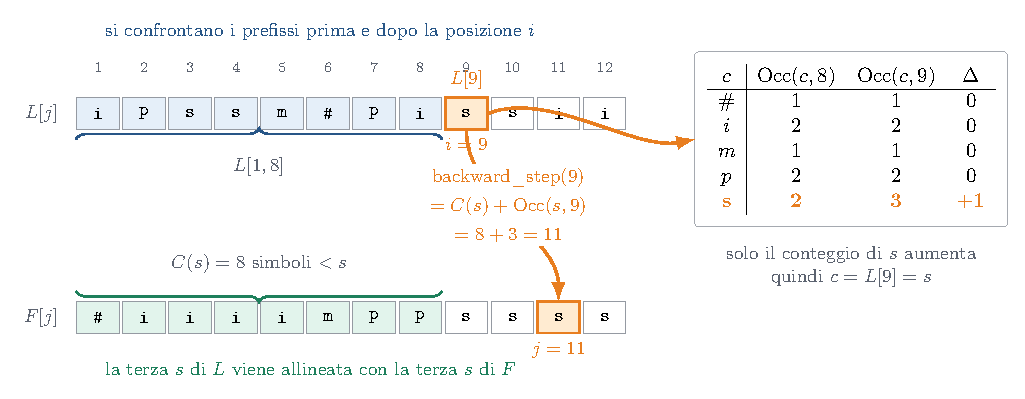
\includegraphics[width=\textwidth]{images/fm-index/backward-step-occ.pdf}
    \caption{Identificazione del carattere $L[i]$ e calcolo del \texten{backward step}. Per $i=9$, il confronto tra $\operatorname{Occ}(c,8)$ e $\operatorname{Occ}(c,9)$ individua $c=s$; la terza occorrenza di $s$ in $L$ viene quindi allineata alla terza occorrenza di $s$ in $F$, alla riga $C(s)+\operatorname{Occ}(s,9)=8+3=11$.}
    \label{fig:fm-index-backward-step-occ}
\end{figure}

\paragraph{Campionamento delle righe.}
Per localizzare le occorrenze senza memorizzare tutto il \texten{suffix array}, l'FM-index campiona alcune righe della matrice BWT. Si pone:
\[
    d
    =
    \left\lceil \log^{1+\varepsilon} n\right\rceil,
    \qquad
    0<\varepsilon<1,
\]
e si marcano le righe che corrispondono a suffissi che iniziano in posizioni del testo multiple di $d$. Per ogni riga marcata $r$ si conserva la sua posizione nel testo in una struttura dati apposita che indichiamo con $S_{\operatorname{loc}}$\footnote{Nelle slide questa struttura è indicata semplicemente con $S$.}:
\[
    S_{\operatorname{loc}}(r)=\operatorname{pos}(r).
\]
Per visualizzare il campionamento, consideriamo di nuovo:
\[
    T=\texttt{mississippi\#}.
\]
Nel piccolo esempio scegliamo $d=4$, così le posizioni testuali campionate sono le multiple di $4$:
\begin{center}
    \small
    \setlength{\tabcolsep}{4pt}
    \begin{tabular}{c|cccccccccccc}
        \textbf{posizione} &
        $1$                & $2$        & $3$        & \textcolor{red}{$4$}         &
        $5$                & $6$        & $7$        & \textcolor{red}{$8$}         &
        $9$                & $10$       & $11$       & \textcolor{red}{$12$}          \\
        \hline
        $T$                &
        \texttt{m}         & \texttt{i} & \texttt{s} & \textcolor{red}{\texttt{s}}  &
        \texttt{i}         & \texttt{s} & \texttt{s} & \textcolor{red}{\texttt{i}}  &
        \texttt{p}         & \texttt{p} & \texttt{i} & \textcolor{red}{\texttt{\#}}   \\
        \textbf{campione}  &
                           &            &            & \textcolor{red}{$\star$}     &
                           &            &            & \textcolor{red}{$\star$}     &
                           &            &            & \textcolor{red}{$\star$}
    \end{tabular}
\end{center}
Queste sono posizioni nel testo, non righe consecutive della matrice BWT. Nell'ordine lessicografico dei suffissi, infatti, i campioni corrispondenti diventano\footnote{Le righe della matrice BWT sono ordinate lessicograficamente e la prima colonna $F$ conserva questo stesso ordine: alla riga $r$ corrisponde quindi la cella $F[r]$. L'indice $r$ identifica la riga, e dunque il suffisso nell'ordine lessicografico, mentre $S_{\operatorname{loc}}(r)=\operatorname{pos}(r)$ conserva la posizione iniziale di quel suffisso nel testo originale.}:
\[
    S_{\operatorname{loc}}(10)=4,
    \qquad
    S_{\operatorname{loc}}(3)=8,
    \qquad
    S_{\operatorname{loc}}(1)=12.
\]
Nel seguito useremo soprattutto il primo di questi campioni, cioè $S_{\operatorname{loc}}(10)=4$.


\paragraph{Algoritmo di localizzazione.}
Se la riga $i$ è marcata, la sua posizione si legge direttamente da $S_{\operatorname{loc}}$. Se non è marcata, si applica ripetutamente il \texten{backward step} descritto nell'Algoritmo~\ref{alg:fm_backward_step}: ogni passo porta a una riga che rappresenta il suffisso spostato di una posizione verso sinistra nel testo. Quando si raggiunge una riga marcata, basta sommare il numero di passi fatti.

\begin{algorithm}[H]
    \caption{Localizzazione di una riga nell'FM-index}
    \label{alg:fm_locate_row}
    \begin{algorithmic}[1]
        \Require riga $i$, struttura dei campioni $S_{\operatorname{loc}}$, procedura $\operatorname{backward\_step}$ dell'Algoritmo~\ref{alg:fm_backward_step}
        \Ensure posizione $\operatorname{pos}(i)$ nel testo
        \State $r\gets i$
        \State $t\gets 0$
        \While{$r$ non è marcata}
        \State $r\gets \operatorname{backward\_step}(r)$
        \State $t\gets t+1$
        \EndWhile
        \State \Return $S_{\operatorname{loc}}(r)+t \pmod n$
    \end{algorithmic}
\end{algorithm}

\paragraph{Esempio.}
Nel caso di \texttt{mississippi\#}, la \texten{backward search} per $P=\texttt{si}$ restituisce l'intervallo $[\textit{First},\textit{Last}]=[9,10]$. Supponiamo che la riga $10$ sia marcata e che:
\[
    S_{\operatorname{loc}}(10)=\operatorname{pos}(10)=4.
\]
Quindi una delle due occorrenze è già localizzata: parte dalla posizione $4$ del testo.

Per la riga $9$, invece, si procede con i \texten{backward step}:
\[
    9
    \xrightarrow{\operatorname{backward\_step}}
    11
    \xrightarrow{\operatorname{backward\_step}}
    4
    \xrightarrow{\operatorname{backward\_step}}
    10.
\]
Dopo $t=3$ passi si raggiunge la riga marcata $10$. Poiché ogni \texten{backward step} ha spostato la posizione testuale indietro di una unità, la posizione originaria della riga $9$ si recupera sommando i passi:
\[
    \operatorname{pos}(9)
    =
    \operatorname{pos}(10)+3
    =
    4+3
    =
    7.
\]
Le due occorrenze di \texttt{si} sono quindi nelle posizioni a partire da $4$ e $7$ del testo $T$.

\paragraph{Analisi.}
Poiché le righe marcate corrispondono a posizioni del testo distanti al più $d=\lceil\log^{1+\varepsilon}n\rceil$, dopo al massimo $d$ \texten{backward step} si raggiunge una riga marcata. Se il test ``$r$ è marcata?'' e l'accesso a $S_{\operatorname{loc}}$ costano $O(1)$, e se anche $\operatorname{backward\_step}$ costa $O(1)$, allora localizzare una singola riga costa:
\begin{equation}\label{eq:fm_marked_rows_bound}
    O(\log^{1+\varepsilon} n).
\end{equation}
Quindi, se il pattern compare $\operatorname{occ}$ volte, la localizzazione di tutte le occorrenze richiede:
\[
    O\!\left(\operatorname{occ}\log^{1+\varepsilon} n\right),
\]
oltre al tempo $O(p)$ necessario per il conteggio.

Il parametro $\varepsilon$ controlla il compromesso spazio-tempo. Le righe marcate sono circa:
\[
    O\!\left(\frac{n}{\log^{1+\varepsilon}n}\right),
\]
e per ciascuna si conserva una posizione del testo, cioè $O(\log n)$ bit. Lo spazio dei campioni è quindi:
\[
    O\!\left(\frac{n}{\log^\varepsilon n}\right)
    \text{ bit}.
\]
Aumentare $\varepsilon$ riduce il numero di campioni e quindi lo spazio, ma aumenta il numero massimo di \texten{backward step} necessari per localizzare una posizione.

\subsubsection{Come calcolare Occ senza decomprimere}
La difficoltà vera è implementare $\operatorname{Occ}(c,q)$ senza conservare tutta la matrice e, nella versione compressa, senza conservare nemmeno esplicitamente la colonna $L$. Dopo la pipeline descritta in precedenza, infatti, l'indice dispone principalmente della stringa di bit $Z$, non di $L$ già pronta da scandire. Tuttavia sia la \texten{backward search} sia il \texten{backward step} richiedono continuamente valori della forma:
\[
    \operatorname{Occ}(c,q)
    =
    |\{j\leq q:L[j]=c\}|.
\]

Il problema diventa quindi: \textbf{come contare le occorrenze di un carattere nei primi $q$ simboli di $L$ leggendo soltanto una quantità costante di informazioni ausiliarie e un piccolo blocco di $Z$?}

Dire che il calcolo avviene ``senza decomprimere'' non significa che nessun bit venga mai decodificato. Significa che non si ricostruiscono né l'intero testo $T$ né l'intera BWT $L$: al più si identifica il piccolo blocco compresso che contiene la posizione $q$ e se ne ricava il contributo locale mediante una tabella precalcolata.

\paragraph{Partizione in bucket e superblocchi.}
Si sceglie una lunghezza:
\[
    \ell=\Theta(\log n)
\]
e si divide logicamente $L$ in \textbf{\texten{bucket}} di $\ell$ caratteri:
\[
    BL_i
    =
    L[(i-1)\ell+1..i\ell],
    \qquad
    i=1,\ldots,\left\lceil\frac{n}{\ell}\right\rceil.
\]
Gruppi di $\ell$ bucket consecutivi formano un \textbf{superblocco}, che contiene quindi $\ell^2=\Theta(\log^2 n)$ caratteri di $L$. Per semplicità si assume che $\ell$ divida $n$; un eventuale ultimo bucket incompleto si tratta allo stesso modo. Il termine $BL_i$ indica il bucket prima della compressione. La partizione di $L$ induce una partizione della sequenza MTF ottenuta elaborando $L$ da sinistra verso destra; applicando poi RLE e il codice a prefisso alla porzione associata a ciascun bucket si ottiene il corrispondente blocco compresso $BZ_i$.

I bucket hanno tutti la stessa lunghezza logica in $L$, ma i blocchi $BZ_i$ hanno lunghezze in bit diverse, perché dipendono dal contenuto da comprimere. Per semplificare la costruzione si assume inoltre che ogni run di zeri prodotta dalla MTF sia interamente contenuta in un bucket. In alternativa, bisognerebbe salvare ai confini anche lo stato necessario a continuare una run iniziata nel bucket precedente.

Per una query $\operatorname{Occ}(c,q)$, con $1\leq q\leq n$, si individuano:
\[
    i=\left\lceil\frac{q}{\ell}\right\rceil,
    \qquad
    h=q-(i-1)\ell,
    \qquad
    t=\left\lfloor\frac{i-1}{\ell}\right\rfloor,
    \qquad
    r=i-t\ell.
\]
L'indice $i$ identifica il bucket che contiene $L[q]$, $h$ è il numero di caratteri da considerare dentro quel bucket, $t$ è il numero di superblocchi completi che lo precedono e $r\in\{1,\ldots,\ell\}$ è la posizione locale di $BL_i$ nel superblocco corrente. Il prefisso $L[1..q]$ viene così diviso in tre parti:
\begin{enumerate}
    \item i primi $t$ superblocchi completi, cioè $L[1..t\ell^2]$;
    \item i bucket completi del superblocco corrente che precedono $BL_i$;
    \item il prefisso $BL_i[1..h]$ del bucket contenente $q$.
\end{enumerate}
La struttura per $\operatorname{Occ}$ deve calcolare separatamente questi tre contributi e poi sommarli.

\paragraph{Conteggi ai confini dei blocchi.}
Per non ricontare ogni volta i caratteri già attraversati si memorizzano due livelli di somme prefisse:
\begin{itemize}
    \item $NO_t[c]$ è il numero di occorrenze di $c$ nei primi $t$ superblocchi, quindi in $L[1..t\ell^2]$; per convenzione $NO_0[c]=0$;
    \item $NO'_{t,r-1}[c]$ conta le occorrenze di $c$ nei primi $r-1$ bucket del superblocco corrente; per convenzione $NO'_{t,0}[c]=0$.
\end{itemize}
Il primo valore risponde alla parte 1 della decomposizione, mentre il secondo risponde alla parte 2. Entrambi si ottengono con un singolo accesso a una tabella.

Il doppio livello è essenziale per lo spazio. Salvare un conteggio globale per ogni bucket richiederebbe $\Theta(\log n)$ bit per ogni contatore; dentro un singolo superblocco, invece, ciascuna cella di $NO'$ contiene un valore non superiore a $\ell^2$, quindi per rappresentare una cella bastano:
\[
    O(\log \ell^2)=O(\log\log n)
\]
bit. Questo bound riguarda quindi \textbf{un singolo contatore relativo di $NO'$}, non l'intera struttura. \uline{I superblocchi forniscono dunque pochi contatori grandi, mentre i bucket forniscono molti contatori piccoli}.

\paragraph{Come trovare il bucket compresso in \(Z\).}
La posizione logica di $BL_i$ non permette di conoscere direttamente la posizione di $BZ_i$ in $Z$, perché i blocchi compressi hanno lunghezza variabile. Si usano perciò altre due somme prefisse:
\begin{itemize}
    \item $W[t]$ è il numero complessivo di bit occupati in $Z$ dai primi $t$ superblocchi compressi;
    \item $W'[t,r-1]$ è il numero di bit occupati dai primi $r-1$ bucket compressi del superblocco corrente; per convenzione $W'[t,0]=0$.
\end{itemize}
Il primo bit di $BZ_i$ si trova quindi nella posizione:
\begin{equation}\label{eq:fm_occ_bucket_start}
    W[t]+W'[t,r-1]+1.
\end{equation}
La lunghezza di $BZ_i$ si ricava da $W'[t,r]-W'[t,r-1]$, poiché $W'[t,r]$ include anche il bucket corrente. In questo modo si estrae da $Z$ esattamente il blocco necessario, senza scorrere tutti quelli precedenti.

\paragraph{Come interpretare il contenuto di \(BZ_i\).}
Conoscere i bit di $BZ_i$ non è ancora sufficiente. La MTF è una trasformazione con stato: lo stesso valore MTF può indicare caratteri diversi a seconda dell'ordine corrente della lista. Per ogni bucket si salva quindi:
\[
    MTF_i
    =
    \text{stato della lista MTF all'inizio di }BL_i.
\]
La coppia $(BZ_i,MTF_i)$ determina univocamente il bucket originale $BL_i$: il codice a prefisso permette di recuperare i simboli RLE, il RLE ricostruisce la sequenza MTF e lo stato iniziale $MTF_i$ permette di invertire la MTF.

Non si esegue però questa decodifica simbolo per simbolo durante ogni query. Si costruisce una \textbf{tabella universale}:
\[
    S[c,h,BZ_i,MTF_i],
\]
che restituisce direttamente il numero di occorrenze di $c$ nei primi $h$ caratteri del bucket $BL_i$. Gli argomenti $BZ_i$ e $MTF_i$ descrivono completamente il bucket, mentre $c$ e $h$ specificano quale conteggio locale serve.

\paragraph{Formula completa.}
Riunendo i tre contributi si ottiene:
\begin{equation}\label{eq:fm_occ_three_parts}
    \operatorname{Occ}(c,q)
    =
    \underbrace{NO_t[c]}_{\text{superblocchi completi}}
    +
    \underbrace{NO'_{t,r-1}[c]}_{\text{bucket completi}}
    +
    \underbrace{S[c,h,BZ_i,MTF_i]}_{\text{prefisso del bucket}}.
\end{equation}
La procedura operativa è quindi:
\begin{enumerate}
    \item calcolare $i$, $h$, $t$ e $r$ con operazioni aritmetiche;
    \item leggere $NO_t[c]$ e $NO'_{t,r-1}[c]$;
    \item localizzare $BZ_i$ in $Z$ mediante \eqref{eq:fm_occ_bucket_start};
    \item leggere lo stato $MTF_i$;
    \item ottenere il contributo locale dalla tabella $S$;
    \item sommare i tre valori secondo \eqref{eq:fm_occ_three_parts}.
\end{enumerate}

\paragraph{Esempio completo.}
La \autoref{fig:fm-index-occ-buckets} usa valori piccoli soltanto per rendere visibile la struttura. Si pone $\ell=4$, quindi ogni bucket contiene $4$ caratteri e ogni superblocco ne contiene $\ell^2=16$. Consideriamo:
\[
    L=\texttt{abacaabbccaabacaabbacaac}.
\]
I blocchi $BZ_i$ mostrati nella figura sono quelli ottenuti usando la lista MTF iniziale $(\texttt{a},\texttt{b},\texttt{c})$ e i codici RLE e a prefisso definiti in precedenza.
Vogliamo calcolare $\operatorname{Occ}(\texttt{a},22)$. Si ha:
\[
    i=\left\lceil\frac{22}{4}\right\rceil=6,
    \qquad
    h=22-(6-1)4=2,
    \qquad
    t=\left\lfloor\frac{6-1}{4}\right\rfloor=1,
    \qquad
    r=6-1\cdot4=2.
\]

Prima di sommare i tre contributi, vediamo esplicitamente come si ottiene quello locale. I primi quattro bucket formano il superblocco completo e occupano:
\[
    W[1]=43
\]
bit di $Z$. Nel superblocco corrente, il bucket $BZ_5$ occupa:
\[
    W'[1,1]=10
\]
bit, mentre $BZ_5$ e $BZ_6$ insieme ne occupano $W'[1,2]=21$. Di conseguenza, usando \eqref{eq:fm_occ_bucket_start}, il primo bit di $BZ_6$ è:
\[
    43+10+1=54,
\]
e la sua lunghezza è:
\[
    W'[1,2]-W'[1,1]=21-10=11
\]
bit. Dunque non si assume di avere già $BL_6$: dalla rappresentazione compressa si estrae soltanto:
\[
    BZ_6
    =
    Z[54..64]
    =
    \texttt{01101010010}.
\]
Separando i codici a prefisso si ottiene:
\[
    \texttt{011}\mid\texttt{010}\mid\texttt{10}\mid\texttt{010}
    \quad\longrightarrow\quad
    2,1,\mathtt{run0},1
    \quad\longrightarrow\quad
    2,1,0,1.
\]
L'ultimo passaggio inverte il RLE: $\mathtt{run0}$ rappresenta una run formata da un solo zero. Lo stato salvato all'inizio del bucket è:
\[
    MTF_6=(\texttt{a},\texttt{b},\texttt{c}).
\]
Invertendo la MTF sui valori $2,1,0,1$ si ricostruisce localmente:
\[
    \begin{array}{c|c|c|c}
        \textbf{valore MTF} & \textbf{lista prima}               & \textbf{carattere} & \textbf{lista dopo}                \\
        \hline
        2                   & (\texttt{a},\texttt{b},\texttt{c}) & \texttt{c}         & (\texttt{c},\texttt{a},\texttt{b}) \\
        1                   & (\texttt{c},\texttt{a},\texttt{b}) & \texttt{a}         & (\texttt{a},\texttt{c},\texttt{b}) \\
        0                   & (\texttt{a},\texttt{c},\texttt{b}) & \texttt{a}         & (\texttt{a},\texttt{c},\texttt{b}) \\
        1                   & (\texttt{a},\texttt{c},\texttt{b}) & \texttt{c}         & (\texttt{c},\texttt{a},\texttt{b})
    \end{array}
\]
e quindi:
\[
    BL_6=\texttt{caac}.
\]
Poiché $h=2$, interessa soltanto il prefisso \texttt{ca}, che contiene una occorrenza di \texttt{a}. Questa decodifica locale serve a capire il contenuto della tabella universale: \uline{durante la query reale non viene ripetuta passo per passo}, ma il valore:
\[
    S[\texttt{a},2,BZ_6,MTF_6]=1
\]
\uline{viene letto direttamente dalla tabella precalcolata}.

Il prefisso $L[1..22]$ contiene quindi:
\begin{itemize}
    \item il primo superblocco completo $BL_1\cdots BL_4$, con $NO_1[\texttt{a}]=8$;
    \item il bucket completo $BL_5=\texttt{abba}$, con $NO'_{1,1}[\texttt{a}]=2$;
    \item il prefisso di lunghezza $h=2$ di $BL_6$, il cui contributo locale appena ricavato è pari a $1$.
\end{itemize}
Pertanto:
\[
    \operatorname{Occ}(\texttt{a},22)
    =
    8+2+1
    =
    11.
\]
La parte inferiore della figura mostra anche perché servono $W$ e $W'$: benché $BL_1,\ldots,BL_6$ abbiano tutti quattro caratteri, i corrispondenti $BZ_i$ occupano numeri diversi di bit.

\begin{figure}[H]
    \centering
    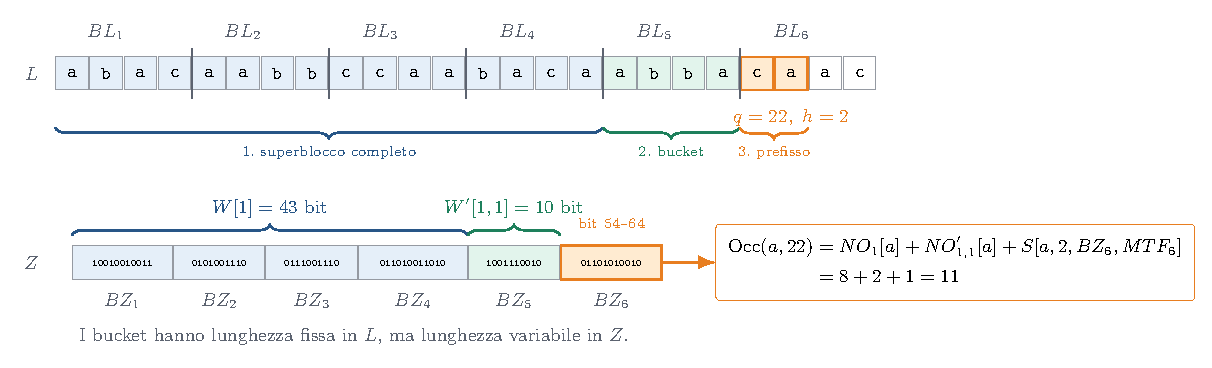
\includegraphics[width=\textwidth]{images/fm-index/occ-buckets.pdf}
    \caption{Calcolo di $\operatorname{Occ}(\texttt{a},22)$ mediante un superblocco completo, un bucket completo e un prefisso del bucket corrente. I bit dei blocchi $BZ_i$ derivano dalla codifica effettiva della BWT di esempio; le strutture $W$ e $W'$ trasformano il numero logico del bucket nella posizione del corrispondente blocco a lunghezza variabile dentro $Z$.}
    \label{fig:fm-index-occ-buckets}
\end{figure}

\paragraph{Costo delle strutture ausiliarie.}
Per evitare ambiguità, in questa analisi indichiamo con $\#X$ il \textbf{numero di celle} della struttura $X$ e con $\operatorname{space}(X)$ il suo \textbf{spazio complessivo in bit}. Ogni stima viene ottenuta come:
\[
    \operatorname{space}(X)
    =
    \#X
    \cdot
    \text{bit necessari per una cella}.
\]
Assumiamo che l'alfabeto $\Sigma$ abbia dimensione costante e ricordiamo che $\ell=\Theta(\log n)$.

\begin{itemize}
    \item \textbf{Contatori globali $NO$.} Esistono $O(n/\ell^2)$ superblocchi e, per ciascuno, si conservano $|\Sigma|$ contatori. Ogni contatore può arrivare fino a $n$ e richiede quindi $O(\log n)$ bit:
          \[
              \#NO
              =
              O\!\left(\frac{n}{\ell^2}|\Sigma|\right),
              \qquad
              \operatorname{space}(NO)
              =
              O\!\left(\frac{n}{\ell^2}|\Sigma|\log n\right)
              =
              O\!\left(\frac{n}{\log n}\right).
          \]

    \item \textbf{Offset globali $W$.} Si conserva un offset per ciascun superblocco, dunque $\#W=O(n/\ell^2)$. Un offset è una posizione in $Z$ e richiede $O(\log n)$ bit:
          \[
              \operatorname{space}(W)
              =
              O\!\left(\frac{n}{\ell^2}\log n\right)
              =
              O\!\left(\frac{n}{\log n}\right).
          \]

    \item \textbf{Contatori relativi $NO'$.} Esistono $O(n/\ell)$ bucket e per ogni confine si conservano $|\Sigma|$ contatori. Ogni valore conta soltanto dentro un superblocco, quindi è al più $\ell^2$ e occupa $O(\log\ell)=O(\log\log n)$ bit:
          \[
              \#NO'
              =
              O\!\left(\frac{n}{\ell}|\Sigma|\right),
              \qquad
              \operatorname{space}(NO')
              =
              O\!\left(\frac{n}{\ell}|\Sigma|\log\ell\right)
              =
              O\!\left(\frac{n\log\log n}{\log n}\right).
          \]

    \item \textbf{Offset relativi $W'$.} Anche $W'$ contiene un valore per bucket, quindi $\#W'=O(n/\ell)$. L'offset misura una posizione interna a un solo superblocco compresso, la cui lunghezza massima è $O(\ell^2)$ bit; ogni cella di $W'$ richiede perciò $O(\log\ell)=O(\log\log n)$ bit:
          \[
              \operatorname{space}(W')
              =
              O\!\left(\frac{n}{\ell}\log\ell\right)
              =
              O\!\left(\frac{n\log\log n}{\log n}\right).
          \]

    \item \textbf{Stati $MTF_i$.} Si salva uno stato per ciascuno degli $O(n/\ell)$ bucket. Uno stato è una permutazione dell'alfabeto e occupa $O(|\Sigma|\log|\Sigma|)=O(1)$ bit:
          \[
              \operatorname{space}(MTF)
              =
              O\!\left(\frac{n}{\ell}|\Sigma|\log|\Sigma|\right)
              =
              O\!\left(\frac{n}{\log n}\right).
          \]
\end{itemize}

Resta da analizzare separatamente la \textbf{tabella universale $S$}. Un bucket compresso ha lunghezza massima:
\[
    b_{\max}
    =
    \ell\bigl(1+2\lfloor\log|\Sigma|\rfloor\bigr)
    \text{ bit}.
\]
Si sceglie la costante nascosta in $\ell=\Theta(\log n)$ in modo che:
\[
    b_{\max}
    =
    \alpha\log n,
    \qquad
    0<\alpha<1.
\]
Il numero di possibili stringhe binarie $BZ_i$ di lunghezza non superiore a $b_{\max}$ è:
\[
    O(2^{b_{\max}})
    =
    O(2^{\alpha\log n})
    =
    O(n^\alpha).
\]
Gli altri indici di $S[c,h,BZ_i,MTF_i]$ hanno:
\begin{itemize}
    \item $|\Sigma|=O(1)$ possibili caratteri $c$;
    \item $\ell=O(\log n)$ possibili lunghezze $h$;
    \item al più $|\Sigma|!=O(1)$ possibili stati MTF.
\end{itemize}
Di conseguenza, il numero di celle della tabella è:
\[
    \#S
    =
    O\!\left(
    |\Sigma|
    \cdot
    \ell
    \cdot
    n^\alpha
    \cdot
    |\Sigma|!
    \right)
    =
    O(n^\alpha\log n).
\]
Ogni cella contiene un conteggio compreso tra $0$ e $\ell$, quindi richiede $O(\log\ell)=O(\log\log n)$ bit. Pertanto:
\[
    \operatorname{space}(S)
    =
    \underbrace{O(n^\alpha\log n)}_{\text{numero di celle}}
    \cdot
    \underbrace{O(\log\log n)}_{\text{bit per cella}}
    =
    O\!\left(n^\alpha\log n\log\log n\right).
\]
\uline{Il fattore $\log\log n$ appartiene allo spazio in bit, non al numero di celle di $S$}. Inoltre, per ogni costante $\alpha<1$:
\[
    \frac{
        n^\alpha\log n\log\log n
    }{
        n\log\log n/\log n
    }
    =
    \frac{\log^2 n}{n^{1-\alpha}}
    \longrightarrow
    0,
\]
e quindi:
\[
    \operatorname{space}(S)
    =
    o\!\left(\frac{n\log\log n}{\log n}\right).
\]
La tabella universale è dunque asintoticamente più piccola delle strutture relative $NO'$ e $W'$.

\paragraph{Riepilogo dei costi.}
Considerando soltanto le strutture ausiliarie necessarie a $\operatorname{Occ}$, e non ancora la stringa compressa $Z$, si ha:
\begin{itemize}
    \item $NO$ e $W$ occupano ciascuna $O(n/\log n)$ bit;
    \item $NO'$ e $W'$ occupano ciascuna $O(n\log\log n/\log n)$ bit e costituiscono il termine dominante;
    \item gli stati MTF occupano complessivamente $O(n/\log n)$ bit;
    \item la tabella universale $S$ occupa $O(n^\alpha\log n\log\log n)$ bit, che è $o(n\log\log n/\log n)$ per $\alpha<1$.
\end{itemize}
Questi sono \textbf{spazi complessivi in bit}, non numeri di celle. Sommando i quattro contributi:
\[
    \operatorname{space}(NO,NO',W,W',MTF,S)
    =
    O\!\left(\frac{n\log\log n}{\log n}\right)
    \text{ bit}.
\]

Tutte le operazioni della query sono accessi diretti a tabelle e parole di macchina. Nel modello RAM con parola di $\Theta(\log n)$ bit e alfabeto costante si ottiene:
\[
    \operatorname{Occ}(c,q)\text{ in tempo }O(1)
\]
Aggiungendo la stringa compressa $Z$, lo spazio della componente dell'indice che supporta il conteggio è:
\begin{equation}\label{eq:fm_occ_space}
    |Z|
    +
    O\!\left(\frac{n\log\log n}{\log n}\right)
    \text{ bit}.
\end{equation}
Questo è il risultato tecnico che rende effettivamente lineare in $p$ la \texten{backward search}: senza questa implementazione, l'ipotesi di accesso costante a $\operatorname{Occ}$ rimarrebbe ingiustificata.

Il termine \eqref{eq:fm_occ_space} va infine combinato con lo spazio dei campioni usati per la localizzazione:
\[
    \operatorname{space}(\text{campioni})
    =
    O\!\left(\frac{n}{\log^\varepsilon n}\right)
\]
bit. Per ogni costante $0<\varepsilon<1$ vale:
\[
    \frac{n\log\log n}{\log n}
    =
    o\!\left(\frac{n}{\log^\varepsilon n}\right),
\]
quindi il costo delle strutture per $\operatorname{Occ}$ viene assorbito dal termine dei campioni. Si ottiene così il limite complessivo enunciato nel teorema seguente.

\begin{theorem}[Ferragina-Manzini]
    Per ogni testo $T[1..n]$, per ogni $k\geq 0$ fissato e per ogni costante $0<\varepsilon<1$, esiste un indice compresso che conta le occorrenze di un pattern $P[1..p]$ in tempo $O(p)$ e localizza tutte le $\operatorname{occ}$ occorrenze in tempo:
    \[
        O\!\left(p+\operatorname{occ}\log^{1+\varepsilon}n\right).
    \]
    Lo spazio è:
    \[
        5nH_k(T)+O\!\left(\frac{n}{\log^\varepsilon n}\right)
    \]
    bit, dove il termine additivo raccoglie le strutture ausiliarie per $\operatorname{Occ}$ e per il campionamento delle righe.
\end{theorem}

Il significato del teorema è forte: l'indice non è solo più piccolo del \texten{suffix array}, ma ha dimensione controllata dall'entropia empirica del testo. Quando il testo è molto comprimibile, l'indice può essere vicino alla dimensione del testo compresso e permettere comunque la ricerca.

\subsubsection{Testi ripetitivi e r-index}
Molte collezioni moderne non sono soltanto comprimibili in senso statistico: sono \textbf{altamente ripetitive}. Succede, per esempio, in pangenomi, versioni successive di pagine web, archivi software e collezioni di documenti quasi uguali. In questi casi l'entropia empirica non sempre cattura tutta la ridondanza utile, perché la caratteristica dominante è la presenza di lunghe ripetizioni tra copie simili.

Una misura molto efficace per questi testi è il numero $r$ di \textbf{run} nella BWT. Se:
\[
    L=\operatorname{BWT}(T)
\]
contiene pochi blocchi massimali di caratteri uguali, allora il testo ha una struttura favorevole a indici basati su run. L'\textbf{\texten{r-index}}, descritto da Gagie, Navarro e Prezza, è un'evoluzione dell'FM-index che sfrutta proprio questo parametro: conserva campioni e informazioni ausiliarie vicino agli inizi delle run della BWT, invece di campionare uniformemente rispetto a $n$.

Per esempio, per:
\[
    W=\texttt{AGAAGAAGAG\$}
\]
la BWT è:
\[
    \operatorname{BWT}(W)=\texttt{GGGG\$AAAAAA}.
\]
Questa trasformata ha soltanto tre run:
\[
    \texttt{G}^4,
    \qquad
    \texttt{\$},
    \qquad
    \texttt{A}^6,
\]
quindi $r=3$ anche se $|W|=11$. L'idea dell'r-index è che, in collezioni molto ripetitive, il numero di run può crescere molto più lentamente della lunghezza totale del testo. Invece di conservare molte posizioni distribuite uniformemente, si conservano informazioni vicino agli inizi delle run e si usa la LF-mapping per propagare le posizioni lungo caratteri uguali consecutivi.

L'idea resta la stessa dell'FM-index: si usa la LF-mapping per muoversi tra righe corrispondenti a suffissi vicini. La differenza è che, quando $r\ll n$, le strutture principali dipendono da $r$ più che da $n$. Per collezioni molto ripetitive questo può essere decisivo: si mantiene la possibilità di contare e localizzare pattern lavorando direttamente sulla rappresentazione compressa, ma lo spazio segue meglio la ridondanza reale della collezione.
























\section{Compressione basata su dizionario}
Gli algoritmi studiati finora comprimono soprattutto tramite modelli probabilistici o trasformazioni che rendono più semplice una successiva codifica statistica. Huffman e la codifica aritmetica richiedono una distribuzione, stimata o nota, dei simboli; la BWT riorganizza il testo per creare contesti più favorevoli a MTF, RLE e codificatori di ordine zero. Queste tecniche funzionano molto bene quando le statistiche della sorgente sono disponibili, stabili o stimabili con un costo accettabile.

In molte situazioni pratiche, però, questa ipotesi è debole. La sorgente può essere sconosciuta, non stazionaria, troppo irregolare, oppure può contenere dipendenze a lunga distanza che non emergono osservando solo le frequenze dei singoli simboli. In questi casi costruire un buon modello probabilistico può essere costoso o poco affidabile: se il modello è povero, anche un codificatore teoricamente molto efficiente finisce per comprimere male.

I \textbf{compressori basati su dizionario}, invece, partono da un'altra idea: se una sottostringa è già comparsa, non conviene riscriverla per intero, ma si può sostituirla con un riferimento. La ridondanza non viene quindi descritta primariamente come una distribuzione di probabilità, ma come \textbf{ripetizione di frasi, parole o blocchi} all'interno dello stesso testo.

Questa famiglia è spesso indicata come famiglia \textbf{Lempel-Ziv} o \textbf{LZ}. Il vantaggio centrale è che non serve conoscere in anticipo la sorgente: la struttura utile viene dedotta dal testo già letto. Per questo motivo i metodi LZ sono particolarmente adatti a testi naturali, codice sorgente, log, file strutturati, archivi con parti ripetute e, più in generale, dati in cui le stesse sottostringhe ricompaiono più volte. Non sono però automaticamente migliori dei compressori statistici: su testi molto brevi, poco ripetitivi o quasi casuali il costo dei riferimenti può superare il risparmio ottenuto.

Il confronto corretto, quindi, non è ``dizionario contro statistica'' in senso assoluto. I metodi a dizionario sono utili perché imparano localmente dal testo e non richiedono una descrizione preventiva della sorgente; i metodi statistici sono utili perché rappresentano in modo molto compatto simboli o eventi con probabilità sbilanciate. Nei compressori reali le due idee vengono spesso combinate: una fase LZ trova le ripetizioni e una fase Huffman o aritmetica codifica in modo efficiente letterali, lunghezze, distanze o indici.

\begin{definizione}
    Sia $T$ un testo. Un \textbf{dizionario} per $T$ è un insieme di coppie
    \[
        D=\{(f,c)\mid f\in F,\ c\in C\},
    \]
    dove $F$ è un insieme di fattori, cioè sottostringhe, di $T$, mentre $C$ è l'insieme delle parole di codice associate. La compressione consiste nel sostituire alcune occorrenze dei fattori $f$ con le corrispondenti parole di codice $c$.
\end{definizione}

Un dizionario può essere \textbf{statico}, se è fissato prima della compressione, oppure \textbf{adattivo}, se viene costruito mentre il testo viene letto. Nel primo caso encoder e decoder devono già conoscere lo stesso dizionario, oppure bisogna trasmetterlo insieme al file compresso. Nel secondo caso, invece, il dizionario non viene normalmente trasmesso: il decoder lo ricostruisce perché segue la stessa regola deterministica dell'encoder.

\subsection{Dizionari statici e dizionari dipendenti dal testo}
Un dizionario statico contiene una lista predefinita di stringhe o pattern che si ritengono frequenti. Può essere costruito usando statistiche su testi tipici, ma resta fisso durante codifica e decodifica. Questa scelta è semplice, ma \uline{funziona bene solo se il dizionario è davvero adatto alla sorgente}.

Qui compare il compromesso fondamentale. Se il dizionario è \textbf{indipendente dalla sorgente}, cioè viene scelto una volta per tutte e poi riutilizzato su molti tipi di testo, non bisogna trasmetterlo e il decoder può conoscerlo in anticipo. Però questa indipendenza ha un costo: il dizionario potrebbe contenere frasi frequenti in generale, ma poco utili per il file corrente. Se invece il dizionario è \textbf{dipendente dalla sorgente}, allora può contenere le frasi davvero ricorrenti in quel dominio o in quel testo, e quindi può comprimere meglio; in cambio, bisogna in qualche modo renderlo disponibile anche al decoder.

Il punto non è quindi che un dizionario indipendente comprima meglio. Al contrario, per migliorare il rapporto di compressione conviene che il dizionario sia il più possibile rappresentativo della sorgente. Il problema è pratico: più il dizionario è specializzato, più aumenta il costo di costruirlo, memorizzarlo o trasmetterlo. Gli algoritmi Lempel-Ziv nascono proprio per aggirare questo costo, perché costruiscono un dizionario che dipende dal testo, ma lo fanno in modo sincronizzato tra encoder e decoder.

\subsubsection{Dizionari di digrammi}
Un esempio elementare di dizionario statico è la codifica dei \textbf{digrammi}, cioè coppie di caratteri. Il dizionario contiene tutti i caratteri singoli dell'alfabeto e, in più, alcune coppie frequenti.

Supponiamo di avere l'alfabeto:
\[
    A=\{\texttt{a},\texttt{b},\texttt{c},\texttt{d},\texttt{r}\}
\]
e il seguente dizionario:
\begin{table}[htpb]
    \centering
    \begin{tabular}{c|c||c|c}
        \textbf{Codice} & \textbf{Entrata} & \textbf{Codice} & \textbf{Entrata} \\ \hline
        \texttt{000}    & \texttt{a}       & \texttt{100}    & \texttt{r}       \\
        \texttt{001}    & \texttt{b}       & \texttt{101}    & \texttt{ab}      \\
        \texttt{010}    & \texttt{c}       & \texttt{110}    & \texttt{ac}      \\
        \texttt{011}    & \texttt{d}       & \texttt{111}    & \texttt{ad}
    \end{tabular}
    \caption{Dizionario statico con caratteri singoli e alcuni digrammi.}
    \label{tab:static_digram_dictionary}
\end{table}

Per codificare \texttt{abracadabra}, l'encoder legge due caratteri alla volta. Se la coppia è nel dizionario, emette il codice della coppia; se non lo è, emette il codice del primo carattere e usa il secondo come inizio del prossimo tentativo. In questo caso la scansione è:
\[
    \texttt{ab}\quad \texttt{r}\quad \texttt{ac}\quad \texttt{ad}\quad
    \texttt{ab}\quad \texttt{r}\quad \texttt{a},
\]
quindi l'output è:
\[
    \texttt{101100110111101100000}.
\]

Il limite di questa tecnica è evidente: se le coppie frequenti del testo non sono quelle nel dizionario, la compressione peggiora. Un dizionario costruito per un libro di economia, ad esempio, può essere poco adatto a un articolo sportivo. Si potrebbe allora costruire un dizionario specifico per ogni file, ma questo introduce un costo aggiuntivo, perché il dizionario va memorizzato o trasmesso.

\subsubsection{Perché servono dizionari adattivi}
I dizionari adattivi risolvono questo problema costruendo il dizionario durante la compressione. Il testo già letto diventa la sorgente naturale dei pattern futuri: se una certa frase, parola o sottostringa è comparsa nella parte precedente del file, è ragionevole cercarla anche nella parte successiva.

In questo senso LZ realizza una via intermedia molto importante: il dizionario non è indipendente dal testo, perché nasce proprio dalle ripetizioni del testo corrente; però non deve essere trasmesso come oggetto separato, perché il decoder lo ricostruisce passo dopo passo seguendo la stessa regola dell'encoder. Si ottiene quindi un adattamento alla sorgente senza il costo esplicito di allegare un dizionario già pronto.

L'idea Lempel-Ziv è proprio questa:
\begin{itemize}
    \item il dizionario viene costruito dinamicamente mentre il messaggio viene compresso;
    \item encoder e decoder aggiornano il dizionario nello stesso modo;
    \item non è necessario trasmettere un dizionario esplicito;
    \item le varianti differiscono soprattutto per il tipo di riferimento usato e per le restrizioni su ciò che può essere referenziato.
\end{itemize}

\subsection{LZ77}
L'algoritmo LZ77, introdotto da Ziv e Lempel nel 1977, è alla base di molti compressori pratici, tra cui DEFLATE, gzip e zlib. La sua idea è usare una \textbf{finestra scorrevole} sul testo. La finestra è divisa in due parti:
\begin{itemize}
    \item il \textbf{\texten{search buffer}}, che contiene una porzione già codificata;
    \item il \textbf{\texten{look-ahead buffer}}, che contiene la parte ancora da codificare.
\end{itemize}

Il puntatore $i$ identifica l'inizio del \texten{look-ahead buffer}, cioè la prossima posizione da codificare. Un secondo puntatore $j$ viene usato per indicare l'inizio di una possibile occorrenza precedente dentro il \texten{search buffer}. La distanza tra $i$ e $j$ diventa l'offset del riferimento.

\begin{figure}[htpb]
    \centering
    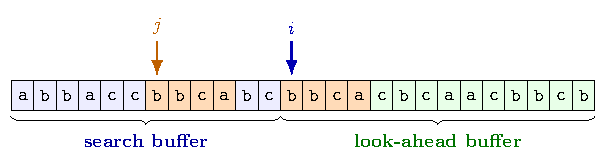
\includegraphics[width=0.82\textwidth]{lz77/lz77-window-overview.pdf}
    \caption{Finestra scorrevole di LZ77. Le celle evidenziate indicano il prefisso del \texten{look-ahead buffer} che compare già nel \texten{search buffer}.}
    \label{fig:lz77_sliding_window_overview}
\end{figure}

In \autoref{fig:lz77_sliding_window_overview} il prefisso
$\alpha=\texttt{bbca}$ del \texten{look-ahead buffer} è già presente nel
\texten{search buffer}. Il puntatore $i$ indica la posizione corrente,
mentre $j$ indica l'occorrenza precedente scelta come riferimento. La
distanza tra $i$ e $j$ è $6$, quindi l'offset è $o=6$; la lunghezza del
match è $\ell=4$ e il simbolo che segue il match è $s=\texttt{c}$. Se
l'encoder sceglie questa occorrenza, emette quindi:
\[
    \langle 6,4,\texttt{c}\rangle.
\]

In generale, alla posizione corrente l'encoder cerca nel \texten{search buffer} la sottostringa più lunga che coincide con un prefisso del \texten{look-ahead buffer}. Se trova un match, lo rappresenta tramite una tripla:
\[
    \langle o,\ell,s\rangle,
\]
dove:
\begin{itemize}
    \item $o$ è l'\textbf{offset}, cioè la distanza all'indietro dall'inizio del match;
    \item $\ell$ è la \textbf{lunghezza} del match;
    \item $s$ è il simbolo che segue il match nel \texten{look-ahead buffer}.
\end{itemize}
Se non c'è nessun match utile, si emette una tripla del tipo $\langle 0,0,s\rangle$, cioè un carattere letterale.

\subsubsection{Algoritmi di codifica e decodifica}
Conviene separare lo schema generale dagli esempi concreti. La
\textbf{codifica} è la parte più costosa: a ogni posizione deve cercare
nel \texten{search buffer} il prefisso più lungo possibile del
\texten{look-ahead buffer}. Dopo avere emesso la tripla, l'encoder avanza
oltre la frase appena rappresentata.

\begin{algorithm}[H]
    \caption{Schema di codifica LZ77}
    \begin{algorithmic}[1]
        \Require testo $S[1..N]$, ampiezza massima della finestra $W$
        \State $p\gets 1$
        \While{$p\leq N$}
        \State cerca il match più lungo di $S[p..]$ in $S[\max(1,p-W)..p-1]$
        \State sia il match a distanza $o$ e lunghezza $\ell$
        \State emetti $\langle o,\ell,S[p+\ell]\rangle$
        \State $p\gets p+\ell+1$
        \EndWhile
    \end{algorithmic}
    \label{alg:lz77_encoding}
\end{algorithm}

La \textbf{decodifica}, invece, non deve cercare nessun match: riceve già
offset e lunghezza. Per ogni tripla copia $\ell$ caratteri dalla posizione
corrente meno $o$, poi aggiunge il simbolo $s$. Per questo il decoder è
molto più semplice e veloce dell'encoder.

\begin{algorithm}[H]
    \caption{Schema di decodifica LZ77}
    \begin{algorithmic}[1]
        \Require sequenza di triple LZ77
        \State $p\gets 1$
        \ForAll{triple $\langle o,\ell,s\rangle$}
        \For{$k=0$ \textbf{to} $\ell-1$}
        \State $S[p+k]\gets S[p-o+k]$
        \EndFor
        \State $S[p+\ell]\gets s$
        \State $p\gets p+\ell+1$
        \EndFor
    \end{algorithmic}
    \label{alg:lz77_decoding}
\end{algorithm}

\subsubsection{Esempio di codifica}
Consideriamo la stringa:
\[
    \texttt{abaababaabb}.
\]
L'encoder procede da sinistra verso destra. A ogni passo guarda il
prefisso ancora da codificare, cerca il match più lungo nel testo già
prodotto e poi emette una tripla. La simulazione completa è:

\begin{center}
    \small
    \renewcommand{\arraystretch}{1.25}
    \begin{tabular}{|c|c|p{0.22\textwidth}|p{0.34\textwidth}|p{0.18\textwidth}|}
        \hline
        \textbf{Passo}                                                                                    & \textbf{$p$} & \textbf{Testo già prodotto} & \textbf{Scelta dell'encoder} & \textbf{Tripla} \\ \hline
        1                                                                                                 & 1            & \emph{vuoto}                &
        nessun match: si emette il letterale \texttt{a}                                                   &
        $\langle 0,0,\texttt{a}\rangle$                                                                                                                                                                 \\ \hline
        2                                                                                                 & 2            & \texttt{a}                  &
        nessun match utile per \texttt{b}: si emette il letterale \texttt{b}                              &
        $\langle 0,0,\texttt{b}\rangle$                                                                                                                                                                 \\ \hline
        3                                                                                                 & 3            & \texttt{ab}                 &
        il prefisso \texttt{a} compare a distanza $2$; si copia \texttt{a} e poi si scrive \texttt{a}     &
        $\langle 2,1,\texttt{a}\rangle$                                                                                                                                                                 \\ \hline
        4                                                                                                 & 5            & \texttt{abaa}               &
        il prefisso \texttt{ba} compare a distanza $3$; si copia \texttt{ba} e poi si scrive \texttt{b}   &
        $\langle 3,2,\texttt{b}\rangle$                                                                                                                                                                 \\ \hline
        5                                                                                                 & 8            & \texttt{abaabab}            &
        il prefisso \texttt{aab} compare a distanza $5$; si copia \texttt{aab} e poi si scrive \texttt{b} &
        $\langle 5,3,\texttt{b}\rangle$                                                                                                                                                                 \\ \hline
    \end{tabular}
\end{center}

La figura seguente visualizza l'ultimo passo della tabella: il
\texten{search buffer} contiene il testo già prodotto, il
\texten{look-ahead buffer} inizia dalla posizione $i$ e il match
\texttt{aab} viene ripreso dalla posizione $j$.

\begin{figure}[htpb]
    \centering
    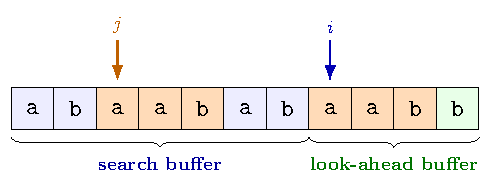
\includegraphics[width=0.62\textwidth]{lz77/lz77-window-example.pdf}
    \caption{Ultimo passo della codifica LZ77 di \texttt{abaababaabb}. Il match evidenziato è \texttt{aab}; il simbolo successivo è \texttt{b}.}
    \label{fig:lz77_encoding_example_last_step}
\end{figure}

Mettendo in fila le triple, si ottiene quindi:
\[
    \langle 0,0,\texttt{a}\rangle\quad
    \langle 0,0,\texttt{b}\rangle\quad
    \langle 2,1,\texttt{a}\rangle\quad
    \langle 3,2,\texttt{b}\rangle\quad
    \langle 5,3,\texttt{b}\rangle.
\]
Le frasi prodotte dalle cinque triple sono, rispettivamente,
\texttt{a}, \texttt{b}, \texttt{aa}, \texttt{bab} e \texttt{aabb}; la
loro concatenazione ricostruisce esattamente \texttt{abaababaabb}.

Un secondo esempio più esteso permette di vedere lo stesso meccanismo su
frasi più lunghe. Consideriamo la stringa\footnote{Ci potrebbe essere una errore nella sequenza di triple
    seguente che ricostruisce \texttt{babbababbaabbaabaabaaa}. Con la variante
    \texttt{babbababbbaabbaabaabaaa}, cioè con una \texttt{b} in più dopo il
    prefisso \texttt{babbaba}, queste triple non tornerebbero.}:
\[
    \texttt{babbababbaabbaabaabaaa}.
\]
Il procedimento è:

\begin{center}
    \scriptsize
    \renewcommand{\arraystretch}{1.25}
    \begin{tabular}{|c|c|p{0.20\textwidth}|p{0.39\textwidth}|p{0.17\textwidth}|}
        \hline
        \textbf{Passo}                                                                                                                 & \textbf{$p$} & \textbf{Testo già prodotto}                   & \textbf{Scelta dell'encoder} & \textbf{Tripla} \\ \hline
        1                                                                                                                              & 1            & \emph{vuoto}                                  &
        nessun match: si emette il letterale \texttt{b}                                                                                &
        $\langle 0,0,\texttt{b}\rangle$                                                                                                                                                                                                                \\ \hline
        2                                                                                                                              & 2            & \texttt{b}                                    &
        nessun match utile per \texttt{a}: si emette il letterale \texttt{a}                                                           &
        $\langle 0,0,\texttt{a}\rangle$                                                                                                                                                                                                                \\ \hline
        3                                                                                                                              & 3            & \texttt{ba}                                   &
        il prefisso \texttt{b} compare a distanza $2$; si copia \texttt{b} e poi si scrive \texttt{b}, producendo \texttt{bb}          &
        $\langle 2,1,\texttt{b}\rangle$                                                                                                                                                                                                                \\ \hline
        4                                                                                                                              & 5            & \texttt{babb}                                 &
        il prefisso \texttt{ab} compare a distanza $3$; si copia \texttt{ab} e poi si scrive \texttt{a}, producendo \texttt{aba}       &
        $\langle 3,2,\texttt{a}\rangle$                                                                                                                                                                                                                \\ \hline
        5                                                                                                                              & 8            & \texttt{babbaba}                              &
        il prefisso \texttt{bba} compare a distanza $5$; si copia \texttt{bba} e poi si scrive \texttt{a}, producendo \texttt{bbaa}    &
        $\langle 5,3,\texttt{a}\rangle$                                                                                                                                                                                                                \\ \hline
        6                                                                                                                              & 12           & \texttt{babbababbaa}                          &
        il prefisso \texttt{bbaa} compare a distanza $4$; si copia \texttt{bbaa} e poi si scrive \texttt{b}, producendo \texttt{bbaab} &
        $\langle 4,4,\texttt{b}\rangle$                                                                                                                                                                                                                \\ \hline
        7                                                                                                                              & 17           & \texttt{babbabab}\allowbreak\texttt{baabbaab} &
        a distanza $3$ si copia progressivamente \texttt{aabaa} e poi si scrive \texttt{a}, producendo \texttt{aabaaa}                 &
        $\langle 3,5,\texttt{a}\rangle$                                                                                                                                                                                                                \\ \hline
    \end{tabular}
\end{center}

Mettendo in fila le triple, si ottiene:
\[
    \langle 0,0,\texttt{b}\rangle\quad
    \langle 0,0,\texttt{a}\rangle\quad
    \langle 2,1,\texttt{b}\rangle\quad
    \langle 3,2,\texttt{a}\rangle\quad
    \langle 5,3,\texttt{a}\rangle\quad
    \langle 4,4,\texttt{b}\rangle\quad
    \langle 3,5,\texttt{a}\rangle.
\]
Le frasi prodotte sono:
\[
    \texttt{b}\quad
    \texttt{a}\quad
    \texttt{bb}\quad
    \texttt{aba}\quad
    \texttt{bbaa}\quad
    \texttt{bbaab}\quad
    \texttt{aabaaa}.
\]
La loro concatenazione restituisce:
\[
    \texttt{babbababbaabbaabaabaaa}.
\]
Questo secondo esempio mostra bene il comportamento progressivo della finestra:
più testo è stato emesso, più aumentano le possibilità di trovare match lunghi.
In particolare, l'ultimo passo anticipa un dettaglio importante della
decodifica: poiché $\ell=5$ è maggiore dell'offset $o=3$, la copia non è
un blocco già interamente disponibile. I primi caratteri vengono letti dal
testo già prodotto e gli ultimi caratteri vengono letti da ciò che si sta
copiando in quello stesso momento.

\subsubsection{Decodifica e copie auto-referenziali}
La parte delicata della decodifica non è la ricerca del match, ma il modo
in cui viene eseguita la copia. È importante che la copia venga fatta
\textbf{simbolo per simbolo}, non come copia in blocco già completamente
disponibile. Infatti LZ77 permette copie auto-referenziali: il riferimento
può puntare a una zona che si sta ancora producendo.

Più precisamente, se la posizione corrente è $p$, una tripla
$\langle o,\ell,s\rangle$ copia, per $k=0,1,\ldots,\ell-1$, il simbolo in
posizione $p-o+k$. Quando $k<o$, il decoder legge simboli che erano già
presenti prima della tripla; quando invece $k\geq o$, il decoder può
leggere simboli appena scritti dalla stessa copia. Per questo, se
$\ell>o$, il riferimento si comporta come una ripetizione periodica di
periodo $o$.

Per esempio, nell'ultimo passo dell'esempio precedente si aveva
$\langle 3,5,\texttt{a}\rangle$. Prima della tripla, gli ultimi tre simboli
disponibili erano:
\[
    \texttt{aab}.
\]
Con offset $3$ e lunghezza $5$, il decoder copia prima questi tre simboli:
\[
    \texttt{aab}.
\]
Poi deve ancora copiare due simboli, ma a quel punto può leggere ciò che ha
appena prodotto: riparte quindi dalle prime due lettere della stessa copia,
cioè \texttt{aa}. Alla fine aggiunge il simbolo esplicito
$s=\texttt{a}$, ottenendo la frase:
\[
    \underbrace{\texttt{aab}}_{\text{già disponibile}}
    \quad
    \underbrace{\texttt{aa}}_{\text{copiato durante la produzione}}
    \quad
    \texttt{a}
    =
    \texttt{aabaaa}.
\]
In altri termini: il decoder copia \texttt{a}, \texttt{a}, \texttt{b},
poi ricomincia dai simboli appena prodotti, copia ancora \texttt{a},
\texttt{a}, e infine aggiunge la \texttt{a} della terza componente della
tripla.

Un caso ancora più evidente si ottiene con offset $1$. Per esempio:
\[
    \langle 0,0,\texttt{a}\rangle
    \langle 0,0,\texttt{c}\rangle
    \langle 2,1,\texttt{a}\rangle
    \langle 4,2,\texttt{b}\rangle
    \langle 1,10,\texttt{a}\rangle
\]
produce prima:
\[
    \texttt{a},\quad \texttt{c},\quad \texttt{aa},\quad \texttt{acb},
\]
cioè, dopo le prime quattro triple, il testo decodificato è:
\[
    \texttt{acaaacb}.
\]
Ora si deve decodificare l'ultima tripla:
\[
    \langle 1,10,\texttt{a}\rangle.
\]
Il valore $o=1$ dice di copiare dal simbolo immediatamente precedente alla
posizione corrente. All'inizio quel simbolo è l'ultima \texttt{b} di
\texttt{acaaacb}; appena il decoder copia questa \texttt{b}, la nuova
\texttt{b} appena prodotta diventa a sua volta il simbolo precedente e può
essere copiata nel passo successivo. Quindi la copia procede così:
\[
    \begin{array}{c|c|c}
        \textbf{stato prima della tripla} & \textbf{tripla}                & \textbf{frase prodotta} \\ \hline
        \texttt{acaaacb}                  & \langle 1,10,\texttt{a}\rangle & \texttt{bbbbbbbbbba}
    \end{array}
\]
La frase prodotta contiene dieci \texttt{b}, ottenute copiando sempre a
distanza $1$, e poi il simbolo finale \texttt{a}. Il risultato complessivo
della decodifica è quindi:
\[
    \texttt{acaaacb}\,\texttt{bbbbbbbbbba}
    =
    \texttt{acaaacbbbbbbbbbbba}.
\]
Questo è il punto essenziale: il riferimento non deve per forza puntare a
un blocco già interamente scritto prima della tripla. Può anche
``inseguire'' il testo che sta producendo, purché la copia venga eseguita
un simbolo alla volta.

\subsubsection{Finestra, lunghezza massima e fattore di compressione}
In pratica LZ77 limita sia la distanza massima del puntatore sia la lunghezza massima del match. Se la finestra è troppo piccola, si perdono ripetizioni lontane; se è troppo grande, la ricerca del match diventa più costosa. Analogamente, aumentare molto la lunghezza massima dei match può non valere il costo se i match lunghi sono rari.

Un caso istruttivo è quello in cui la compressione può addirittura peggiorare la dimensione. Si codifica:
\[
    \texttt{010020\$0110\$\$0111}
\]
su un alfabeto di dimensione $4$, quindi $2$ bit per carattere. La stringa non compressa usa:
\[
    17\cdot 2=34\ \text{bit}.
\]
Con una finestra di $7$ simboli e match lunghi al massimo $3$, servono $3$ bit per l'offset, $2$ bit per la lunghezza e $2$ bit per il carattere, quindi $7$ bit per tripla. La codifica riportata è:
\[
    \begin{aligned}
         & \langle 0,0,\texttt{0}\rangle
        \langle 0,0,\texttt{1}\rangle
        \langle 2,1,\texttt{0}\rangle
        \langle 0,0,\texttt{2}\rangle     \\
         & \langle 2,1,\texttt{\$}\rangle
        \langle 7,2,\texttt{1}\rangle
        \langle 5,2,\texttt{\$}\rangle
        \langle 6,3,\texttt{1}\rangle.
    \end{aligned}
\]
Ci sono $8$ triple, cioè $8\cdot 7=56$ bit. Il rapporto:
\[
    \frac{34}{56}\simeq 0{,}607
\]
è minore di $1$, quindi in questo esempio il formato compresso è più grande del testo originario. Questo non contraddice il principio dell'algoritmo: mostra solo che il guadagno dipende dalla ripetitività effettiva e dal costo dei riferimenti.

\subsubsection{Parsing ed encoding}
Per LZ77 conviene distinguere due fasi:
\begin{itemize}
    \item il \textbf{parsing}, che trasforma il testo in una sequenza di triple o frasi;
    \item l'\textbf{encoding}, che rappresenta queste triple come bit.
\end{itemize}
La fase di encoding può usare un compressore statistico, come Huffman o codifica aritmetica, sulle componenti delle triple, oppure un codice universale per interi. Questo chiarisce perché molti compressori reali siano ibridi: LZ individua le ripetizioni, poi un codificatore statistico rappresenta in modo compatto letterali, lunghezze e distanze.

La ricerca del prefisso più lungo è il collo di bottiglia dell'encoder. Una ricerca ingenua, che controlla tutte le possibili occorrenze nel \texten{search buffer}, è troppo lenta su file grandi. Il decoder, invece, è molto veloce: deve solo copiare caratteri da posizioni già ricostruite.

\subsubsection{Varianti pratiche di LZ77}
La descrizione vista finora specifica il \textbf{parsing} di LZ77, cioè il modo in cui il testo viene diviso in riferimenti della forma:
\[
    \langle o,\ell,s\rangle.
\]
Non specifica però in modo unico come queste triple debbano essere rappresentate in bit. Questa distinzione è importante perché, nelle implementazioni reali, le tre componenti non hanno tutte lo stesso comportamento statistico. Per ottimizzare la compressione, conviene quindi trattarle in modo diverso, usando codifiche più adatte a ciascuna di esse.
\begin{itemize}
    \item L'\textbf{offset} $o$, indica quanto bisogna tornare indietro nella finestra. In molti testi i match più utili sono spesso abbastanza recenti: parole, frammenti o pattern tendono a ripetersi vicino al punto in cui sono già comparsi. Per questo motivo gli offset piccoli compaiono spesso più degli offset grandi. Codificarli tutti con lo stesso numero di bit può essere uno spreco; conviene invece usare una \textbf{codifica a lunghezza variabile}, assegnando parole di codice più corte agli offset piccoli e parole più lunghe agli offset grandi.
    \item La \textbf{lunghezza} $\ell$ del match. Anche $\ell$ è un intero, e in molti casi valori piccoli sono più frequenti di valori molto grandi. Una variante pratica può quindi usare codici a lunghezza variabile anche per le lunghezze, evitando di pagare sempre il costo massimo previsto dalla finestra.
    \item Il \textbf{simbolo esplicito} $s$, è ancora più delicata. Nella forma base di LZ77 ogni riferimento contiene sempre anche il simbolo successivo al match. Questo è comodo perché garantisce l'avanzamento della codifica, ma non è sempre necessario: se il match è abbastanza lungo, quel simbolo può essere trattato come inizio della frase successiva; se invece non c'è un match utile, scrivere una tripla del tipo $\langle 0,0,c\rangle$ significa pagare due componenti nulle solo per trasmettere un letterale.
\end{itemize}

Per questo alcune varianti aggiungono la terza componente solo quando serve, usando un bit di flag per indicare se essa è presente oppure assente. La variante \textbf{LZss} nasce proprio da questa idea: invece di forzare sempre la forma a tre componenti, distingue tra letterali e riferimenti, rappresentando ciascun caso nel modo più economico.

\subsection{LZss}
Storer e Szymanski proposero nel 1982 una variante di LZ77, chiamata \textbf{LZss}. L'osservazione è che una tripla LZ77 contiene sempre tre componenti, anche quando non tutte sono davvero utili:
\begin{itemize}
    \item se è stato trovato un match lungo, il carattere successivo può essere gestito come inizio della frase successiva, quindi non è sempre necessario aggiungerlo nella stessa tripla;
    \item se non è stato trovato un match, emettere $\langle 0,0,c\rangle$ spreca due componenti nulle.
\end{itemize}

LZss emette quindi sempre una coppia, ma di due tipi:
\[
    \langle d,\ell\rangle
    \quad\text{oppure}\quad
    \langle 0,c\rangle.
\]
Nel primo caso si copia una frase già apparsa a distanza $d$ e lunga $\ell$; nel secondo caso si emette un letterale $c$. Nelle implementazioni reali si usa spesso un bit di flag per distinguere letterali e riferimenti.

Per la stringa:
\[
    \texttt{aabbabab},
\]
una possibile codifica LZss è:
\[
    \langle 0,\texttt{a}\rangle
    \langle 1,1\rangle
    \langle 0,\texttt{b}\rangle
    \langle 1,1\rangle
    \langle 3,2\rangle
    \langle 2,2\rangle.
\]
L'idea è la stessa di LZ77, ma i letterali e i riferimenti sono trattati in modo più economico.

\subsubsection{Confronto tra parsing LZ77 e LZss}
Indichiamo con $z$ il numero di frasi nel parsing LZ77 di una stringa $s$ e con $z'$ il numero di frasi nel parsing LZss. Consideriamo una decomposizione di $s$ in stringhe non vuote:
\[
    s=t_1t_2\cdots t_r
\]
Distinguiamo due tipi di fattorizzazione:
\begin{itemize}
    \item Una fattorizzazione è di tipo \textbf{LZss} se ogni $t_i$ è:
          \begin{itemize}
              \item un singolo carattere;
              \item una stringa che ha un'occorrenza nel prefisso che termina prima dell'ultimo simbolo di $t_i$:
                    \[
                        s[1..|t_1t_2\cdots t_i|-1].
                    \]
          \end{itemize}

    \item Una fattorizzazione è di tipo \textbf{LZ77} se, per ogni frase $t_i$, il prefisso
          \[
              t_i[1..|t_i|-1]
          \]
          ha un'occorrenza nel prefisso
          \[
              s[1..|t_1t_2\cdots t_i|-2].
          \]
          Anche qui l'occorrenza può essere autosovrapposta alla frase corrente, come nella copia progressiva di LZ77.
\end{itemize}

\begin{theorem}[Lempel-Ziv, 1976]
    Per ogni stringa $s$, il numero $z'$ di frasi prodotte dal parsing LZss è minore o uguale alla dimensione di qualunque fattorizzazione di tipo LZss. Analogamente, il numero $z$ di frasi prodotte dal parsing LZ77 è minore o uguale alla dimensione di qualunque fattorizzazione di tipo LZ77.
\end{theorem}

\begin{theorem}[Kosolobov-Shur, 2019]
    Per ogni stringa $s$ vale:
    \[
        \frac{1}{2}z' < z \leq z'.
    \]
\end{theorem}
\begin{proof}
    La disuguaglianza $z\leq z'$ segue dal fatto che una fattorizzazione di tipo LZss è automaticamente anche una fattorizzazione di tipo LZ77. Infatti LZss richiede che sia copiabile tutta la frase, oppure che la frase sia un singolo carattere; LZ77 richiede solo che sia copiabile la frase senza l'ultimo carattere. È quindi una richiesta più debole. Il parsing LZss, che ha $z'$ frasi, è allora una fattorizzazione LZ77 valida; poiché il parsing LZ77 è minimo tra le fattorizzazioni LZ77, deve valere $z\leq z'$.

    Per l'altra disuguaglianza, partiamo invece dal parsing LZ77 di $s$, formato da $z$ frasi. Ogni frase LZ77 può essere vista come:
    \begin{itemize}
        \item una parte iniziale copiata dal testo disponibile;
        \item un carattere finale scritto esplicitamente.
    \end{itemize}
    La parte copiata, se non è vuota, è una frase valida per una fattorizzazione LZss; il carattere finale è comunque valido come letterale. Dunque ogni frase LZ77 può essere sostituita da al più due frasi LZss.

    La prima frase LZ77, però, non può copiare nulla da sinistra, perché all'inizio non esiste testo già disponibile: quindi è necessariamente un solo carattere e contribuisce una sola frase LZss. In totale otteniamo una fattorizzazione LZss con al più $2z-1$ frasi. Per la minimalità del parsing LZss:
    \[
        z' \leq 2z-1 < 2z,
    \]
    da cui segue $\frac{1}{2}z' < z$.
\end{proof}

Il significato è che LZ77 non produce più frasi di LZss, ma il vantaggio non può essere arbitrariamente grande: il numero di frasi LZss è al più quasi il doppio del numero di frasi LZ77.

\subsection{Gzip e DEFLATE}
Gzip è una variante pratica molto importante della famiglia LZ77. Usa l'algoritmo \textbf{DEFLATE}, che combina LZ77 con codifica di Huffman. In modo schematico:
\begin{itemize}
    \item LZ77 produce letterali, lunghezze e distanze;
    \item Huffman codifica in modo compatto questi valori;
    \item l'output finale non contiene triple grezze, ma una rappresentazione statistica dei loro componenti.
\end{itemize}

Il problema implementativo principale è trovare velocemente il prefisso più lungo $\alpha$ del \texten{look-ahead buffer} $B$ che compare nella finestra precedente $W$. Gzip accelera questa ricerca usando una tabella hash di \textbf{3-grammi}:
\begin{enumerate}
    \item si cerca il trigramma $B[1..3]$ nella tabella;
    \item se non esiste, si emette un letterale e si avanza di un carattere;
    \item se esiste, si recuperano le posizioni precedenti in cui il trigramma compare;
    \item da quelle posizioni si estende il confronto per trovare il prefisso comune più lungo;
    \item si sceglie il match migliore e si emette una coppia distanza-lunghezza.
\end{enumerate}

Quando la finestra scorre, la tabella hash deve essere aggiornata: si rimuovono i 3-grammi che escono dalla finestra e si inseriscono quelli che entrano. Le distanze e le lunghezze sono poi codificate con Huffman. In gzip, il formato usa due alfabeti: uno per letterali e lunghezze, e uno per le distanze. Se il decoder legge un letterale, lo emette direttamente; se legge una lunghezza, sa che deve leggere anche una distanza.

La dimensione della finestra è un compromesso. gzip usa una finestra di $32\cdot 2^{10}=32768$ byte, mentre 7-zip può usare finestre molto più grandi, fino a dimensioni dell'ordine di $2^{30}$. Finestre più grandi possono trovare ripetizioni più lontane, ma richiedono più memoria e più tempo di ricerca.

\subsection{LZ78}
LZ78, introdotto da Ziv e Lempel nel 1978, usa un dizionario esplicito di frasi già parsate. A differenza di LZ77, non si può puntare a qualunque sottostringa della finestra: si possono referenziare solo frasi complete già presenti nel dizionario.

Questa restrizione ha due effetti:
\begin{itemize}
    \item evita alcune rappresentazioni ridondanti o parziali tipiche di LZ77;
    \item richiede di mantenere un dizionario vero e proprio, quindi la decodifica usa più memoria ed è meno locale.
\end{itemize}

Il dizionario parte da una frase vuota, con indice $0$. A ogni passo l'encoder cerca il prefisso più lungo già presente nel dizionario, poi emette la coppia:
\[
    \langle \text{indice della frase precedente},\ \text{prossimo carattere}\rangle.
\]
La concatenazione tra la frase precedente e il prossimo carattere diventa una nuova frase del dizionario.

\begin{algorithm}[htpb]
    \caption{Schema di codifica LZ78}
    \begin{algorithmic}[1]
        \Require testo $S$
        \State inizializza $D[0]\gets \epsilon$
        \State $p\gets 1$
        \While{$p\leq |S|$}
        \State sia $w$ il prefisso più lungo di $S[p..]$ presente in $D$
        \State sia $c$ il carattere che segue $w$
        \State emetti $\langle \operatorname{index}(w),c\rangle$
        \State aggiungi $wc$ al dizionario con un nuovo indice
        \State $p\gets p+|w|+1$
        \EndWhile
    \end{algorithmic}
    \label{alg:lz78_encoding}
\end{algorithm}

In parole, LZ78 legge il testo una frase alla volta: cerca la frase già nota più lunga che coincide con il testo corrente, la identifica tramite il suo indice nel dizionario e aggiunge il primo carattere nuovo che la estende. La coppia emessa descrive proprio questi due elementi, mentre la nuova frase viene salvata nel dizionario per i passi successivi.

\subsubsection{Esempio di parsing}
Per la stringa:
\[
    \texttt{abaababaa},
\]
conviene leggere il testo da sinistra a destra, aggiornando il dizionario dopo ogni emissione. Il passo $0$ è già il primo passo di codifica: il dizionario disponibile contiene solo la frase vuota, con indice $0$. A ogni passo si prende il prefisso già noto più lungo $w$, si legge il carattere successivo $c$, si emette $\langle\operatorname{index}(w),c\rangle$ e si aggiunge $wc$ al dizionario:
\begin{table}[htpb]
    \centering
    \small
    \begin{tabular}{l|l|l|l|l}
        \textbf{Passo} & \textbf{Dizionario disponibile}                                      & \textbf{$w$ trovato} & \textbf{Output}               & \textbf{Nuova frase} \\ \hline
        $0$            & $\{\,\}$                                                             & $\epsilon$           & $\langle 0,\texttt{a}\rangle$ & $\texttt{a}$         \\
        $1$            & $\{ 1:\texttt{a}\,\}$                                                & $\epsilon$           & $\langle 0,\texttt{b}\rangle$ & $\texttt{b}$         \\
        $2$            & $\{ 1:\texttt{a},\ 2:\texttt{b}\,\}$                                 & \texttt{a}           & $\langle 1,\texttt{a}\rangle$ & $\texttt{aa}$        \\
        $3$            & $\{ 1:\texttt{a},\ 2:\texttt{b},\ 3:\texttt{aa}\,\}$                 & \texttt{b}           & $\langle 2,\texttt{a}\rangle$ & $\texttt{ba}$        \\
        $4$            & $\{ 1:\texttt{a},\ 2:\texttt{b},\ 3:\texttt{aa},\ 4:\texttt{ba}\,\}$ & \texttt{ba}          & $\langle 4,\texttt{a}\rangle$ & $\texttt{baa}$
    \end{tabular}
    \caption{Costruzione passo-passo del parsing LZ78 di \texttt{abaababaa}.}
    \label{tab:lz78_abaababaa_steps}
\end{table}

In questo modo il primo elemento della coppia è sempre l'indice della frase $w$ nel dizionario disponibile: per esempio, in $\langle 2,\texttt{a}\rangle$ il numero $2$ rimanda alla voce $2:\texttt{b}$, e la nuova frase diventa \texttt{ba}.

Concatenando le nuove frasi prodotte nelle cinque emissioni si recupera il testo originale:
\[
    \texttt{a}\ \texttt{b}\ \texttt{aa}\ \texttt{ba}\ \texttt{baa}
    = \texttt{abaababaa}.
\]
La sequenza di coppie emessa è quindi:
\[
    \langle 0,\texttt{a}\rangle
    \langle 0,\texttt{b}\rangle
    \langle 1,\texttt{a}\rangle
    \langle 2,\texttt{a}\rangle
    \langle 4,\texttt{a}\rangle.
\]
Il dizionario costruito è:
\begin{table}[H]
    \centering
    \begin{tabular}{c|cccccc}
        \textbf{Indice} & $0$        & $1$        & $2$        & $3$         & $4$         & $5$          \\ \hline
        \textbf{Frase}  & $\epsilon$ & \texttt{a} & \texttt{b} & \texttt{aa} & \texttt{ba} & \texttt{baa}
    \end{tabular}
    \caption{Dizionario LZ78 costruito per \texttt{abaababaa}.}
    \label{tab:lz78_abaababaa}
\end{table}

Consideriamo ora un secondo esempio:
\[
    \texttt{aabbababbbaababaa},
\]
il cui parsing LZ78 è:
\[
    \langle 0,\texttt{a}\rangle
    \langle 1,\texttt{b}\rangle
    \langle 0,\texttt{b}\rangle
    \langle 2,\texttt{a}\rangle
    \langle 3,\texttt{b}\rangle
    \langle 3,\texttt{a}\rangle
    \langle 4,\texttt{b}\rangle
    \langle 1,\texttt{a}\rangle.
\]

\subsubsection{Memorizzazione con trie}
Per implementare LZ78 in modo efficiente si usa un \textbf{trie}. La radice rappresenta la frase vuota e ogni cammino dalla radice a un nodo rappresenta una frase del dizionario. Il numero del nodo è l'indice della frase.

Nel caso dell'esempio precedente, il dizionario della \autoref{tab:lz78_abaababaa} può essere rappresentato come nella \autoref{fig:lz78_trie_example}. Per cercare una frase, l'encoder parte dalla radice e segue gli archi etichettati con i caratteri in input. Se il prossimo testo fosse \texttt{baab}, il cammino \texttt{b}\(\to\)\texttt{a}\(\to\)\texttt{a} porterebbe al nodo $5$, cioè alla frase già nota \texttt{baa}; il carattere successivo \texttt{b} non è ancora nel trie, quindi si emette $\langle 5,\texttt{b}\rangle$ e si aggiunge il nuovo nodo \texttt{baab}.

\begin{figure}[htpb]
    \centering
    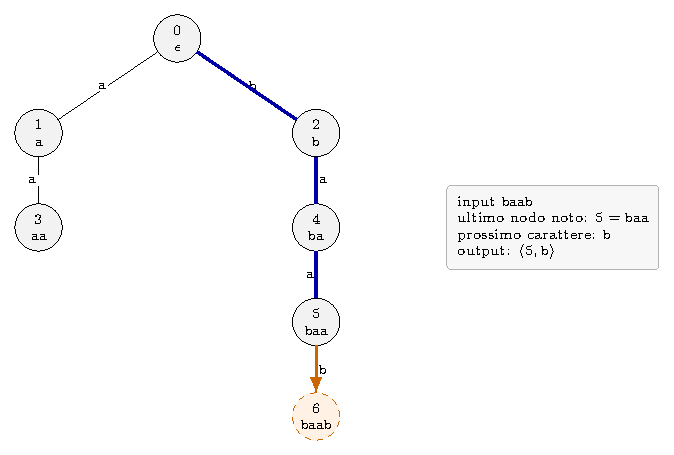
\includegraphics[width=0.78\textwidth]{lz78/lz78-trie-example.pdf}
    \caption{Trie associato al dizionario LZ78 dell'esempio su \texttt{abaababaa}. Il cammino evidenziato mostra come verrebbe codificato il testo successivo \texttt{baab}.}
    \label{fig:lz78_trie_example}
\end{figure}

Durante la codifica:
\begin{itemize}
    \item i caratteri in input vengono usati per scendere nel trie;
    \item l'ultimo nodo raggiunto rappresenta la frase più lunga già nota;
    \item si emette l'indice di quel nodo insieme al prossimo carattere;
    \item si aggiunge un nuovo nodo per rappresentare la frase estesa.
\end{itemize}

\subsubsection{Decodifica LZ78}
La decodifica è simmetrica. Per ogni coppia $\langle i,c\rangle$, il decoder recupera la frase $D[i]$, aggiunge $c$, emette $D[i]c$ e inserisce la stessa nuova frase nel dizionario.

\begin{algorithm}[htpb]
    \caption{Schema di decodifica LZ78}
    \begin{algorithmic}[1]
        \Require sequenza di coppie $\langle i,c\rangle$
        \State inizializza $D[0]\gets \epsilon$
        \ForAll{coppie $\langle i,c\rangle$}
        \State $w\gets D[i]c$
        \State emetti $w$
        \State aggiungi $w$ al dizionario
        \EndFor
    \end{algorithmic}
    \label{alg:lz78_decoding}
\end{algorithm}

Per esempio:
\[
    \langle 0,\texttt{c}\rangle
    \langle 1,\texttt{a}\rangle
    \langle 1,\texttt{c}\rangle
    \langle 0,\texttt{b}\rangle
    \langle 2,\texttt{b}\rangle
    \langle 5,\texttt{a}\rangle
\]
ricostruisce:
\[
    \texttt{c}\quad \texttt{ca}\quad \texttt{cc}\quad \texttt{b}\quad
    \texttt{cab}\quad \texttt{caba},
\]
cioè:
\[
    \texttt{ccacccabcaba}.
\]

\subsubsection{Limiti pratici di LZ78}
Il trie cresce durante la compressione e, se non viene limitato, può occupare molta memoria. Per controllarne la dimensione si usano alcune strategie:
\begin{itemize}
    \item ricostruire il trie da zero quando diventa troppo grande;
    \item congelarlo e continuare a usarlo senza aggiungere nuove frasi;
    \item ricostruirlo parzialmente usando solo dati recenti.
\end{itemize}

Rispetto a LZ77, LZ78 non ha una finestra che impedisce di referenziare pattern molto lontani, ma deve memorizzare frasi esplicite. L'encoding può essere veloce se il trie è ben implementato; il decoding è in genere più pesante perché deve conservare e ricostruire le frasi.

\subsection{LZW}
LZW è una variante di LZ78 proposta da Welch nel 1984. È stata usata in formati e strumenti molto noti, tra cui GIF, TIFF e l'utility Unix \texttt{compress}.

La differenza principale rispetto a LZ78 è che LZW emette \textbf{solo indici di frasi}, senza trasmettere il carattere aggiuntivo. Per rendere possibile questa scelta, il dizionario iniziale contiene già tutti i simboli dell'alfabeto. Le nuove frasi vengono costruite concatenando la frase appena codificata con il primo carattere della frase successiva.

\begin{algorithm}[htpb]
    \caption{Schema di codifica LZW}
    \begin{algorithmic}[1]
        \Require testo $S$, dizionario iniziale con tutti i caratteri dell'alfabeto
        \State $w\gets$ primo carattere di $S$
        \ForAll{caratteri successivi $k$}
        \If{$wk$ è nel dizionario}
        \State $w\gets wk$
        \Else
        \State emetti $\operatorname{code}(w)$
        \State aggiungi $wk$ al dizionario
        \State $w\gets k$
        \EndIf
        \EndFor
        \State emetti $\operatorname{code}(w)$
    \end{algorithmic}
    \label{alg:lzw_encoding}
\end{algorithm}

\subsubsection{Esempio di codifica}
Consideriamo il dizionario iniziale:
\[
    \texttt{a}\mapsto 1,\qquad
    \texttt{b}\mapsto 2,\qquad
    \texttt{c}\mapsto 3
\]
e il testo:
\[
    \texttt{bcababbcbcbaaaabbc}.
\]
La codifica procede cercando ogni volta la frase più lunga $w$ già presente nel dizionario. Quando il carattere successivo $k$ non permette più di estendere $w$, si emette il codice di $w$ e si aggiunge la nuova frase $wk$. Nella tabella seguente, la parte sottolineata è la sequenza appena testata e inserita nel codebook; la parte rossa, invece, è il prefisso già noto di cui viene prodotto il codice in output.
\begin{table}[H]
    \centering
    \small
    \begin{tabular}{c|l|c|l}
        \textbf{Passo} & \textbf{Input corrente}                                                & \textbf{Output} & \textbf{Codebook}                            \\ \hline
        $0$            & \texttt{bcababbcbcbaaaabbc}                                            & --              & $1:\texttt{a},\ 2:\texttt{b},\ 3:\texttt{c}$ \\
        $1$            & \uline{\textcolor{red}{\texttt{b}}\texttt{c}}\texttt{ababbcbcbaaaabbc} & $2$             & $4:\texttt{bc}$                              \\
        $2$            & \uline{\textcolor{red}{\texttt{c}}\texttt{a}}\texttt{babbcbcbaaaabbc}  & $3$             & $5:\texttt{ca}$                              \\
        $3$            & \uline{\textcolor{red}{\texttt{a}}\texttt{b}}\texttt{abbcbcbaaaabbc}   & $1$             & $6:\texttt{ab}$                              \\
        $4$            & \uline{\textcolor{red}{\texttt{b}}\texttt{a}}\texttt{bbcbcbaaaabbc}    & $2$             & $7:\texttt{ba}$                              \\
        $5$            & \uline{\textcolor{red}{\texttt{ab}}\texttt{b}}\texttt{cbcbaaaabbc}     & $6$             & $8:\texttt{abb}$                             \\
        $6$            & \uline{\textcolor{red}{\texttt{bc}}\texttt{b}}\texttt{cbaaaabbc}       & $4$             & $9:\texttt{bcb}$                             \\
        $7$            & \uline{\textcolor{red}{\texttt{bcb}}\texttt{a}}\texttt{aaaabbc}        & $9$             & $10:\texttt{bcba}$                           \\
        $8$            & \uline{\textcolor{red}{\texttt{a}}\texttt{a}}\texttt{aabbc}            & $1$             & $11:\texttt{aa}$                             \\
        $9$            & \uline{\textcolor{red}{\texttt{aa}}\texttt{a}}\texttt{bbc}             & $11$            & $12:\texttt{aaa}$                            \\
        $10$           & \uline{\textcolor{red}{\texttt{abb}}\texttt{c}}                        & $8$             & $13:\texttt{abbc}$                           \\
        $11$           & \textcolor{red}{\texttt{c}}                                            & $3$             & --
    \end{tabular}
    \caption{Passi della codifica LZW di \texttt{bcababbcbcbaaaabbc}.}
    \label{tab:lzw_encoding_bcababb}
\end{table}

Leggendo la colonna degli output si ottiene:
\[
    2,\ 3,\ 1,\ 2,\ 6,\ 4,\ 9,\ 1,\ 11,\ 8,\ 3.
\]
Il passaggio sulla sequenza di \texttt{a} mostra bene come compaiono le frasi \texttt{aa} e \texttt{aaa}; la regola dell'algoritmo resta quella appena descritta.

\subsubsection{Decodifica e caso speciale}
Il decoder parte dallo stesso dizionario iniziale. Dopo aver decodificato una frase corrente $w$, legge il codice successivo. Se il codice è già nel dizionario, lo traduce normalmente; poi aggiunge al dizionario la concatenazione:
\[
    w + \text{primo carattere della frase appena decodificata}.
\]

Esiste però un caso speciale: il decoder può leggere un codice che non è ancora nel dizionario. Questo accade quando l'encoder ha appena creato una frase del tipo:
\[
    w + \operatorname{first}(w).
\]
Allora il decoder può ricostruirla comunque, perché conosce $w$ e conosce il suo primo carattere.

\begin{algorithm}[htpb]
    \caption{Schema di decodifica LZW}
    \begin{algorithmic}[1]
        \Require sequenza di codici LZW
        \State leggi il primo codice e decodificalo come $w$
        \State emetti $w$
        \ForAll{codici successivi $k$}
        \If{$k$ è nel dizionario}
        \State $e\gets D[k]$
        \Else
        \State $e\gets w\,\operatorname{first}(w)$
        \EndIf
        \State emetti $e$
        \State aggiungi $w\,\operatorname{first}(e)$ al dizionario
        \State $w\gets e$
        \EndFor
    \end{algorithmic}
    \label{alg:lzw_decoding}
\end{algorithm}

Per la sequenza:
\[
    2,\ 3,\ 1,\ 2,\ 6,\ 4,\ 9,\ 1,\ 11,\ 8,\ 3
\]
con dizionario iniziale $\texttt{a}=1,\texttt{b}=2,\texttt{c}=3$, possiamo seguire i passaggi in modo parallelo alla codifica. In decodifica, però, la nuova voce non si ottiene concatenando tutta la frase successiva: si usa solo il suo primo carattere. Quindi, se la frase corrente è $w$ e la frase successiva è $e$, il decoder aggiunge
\[
    w\,\operatorname{first}(e).
\]
Nella tabella, il codice rosso è quello decodificato in quel passo; la colonna ``primo carattere successivo'' esplicita quale carattere viene usato per costruire la nuova voce:
\begin{table}[H]
    \centering
    \small
    \begin{tabular}{c|l|c|c|l}
        \textbf{Passo} & \textbf{Codici correnti}                    & \textbf{Output}               & \textbf{Primo car. succ.} & \textbf{Codebook}                                    \\ \hline
        $0$            & $2,3,1,2,6,4,9,1,11,8,3$                    & --                            & --                        & $1:\texttt{a},\ 2:\texttt{b},\ 3:\texttt{c}$         \\
        $1$            & \textcolor{red}{$2$},$3,1,2,6,4,9,1,11,8,3$ & \textcolor{red}{\texttt{b}}   & \texttt{c}                & $4:\uline{\textcolor{red}{\texttt{b}}\texttt{c}}$    \\
        $2$            & \textcolor{red}{$3$},$1,2,6,4,9,1,11,8,3$   & \textcolor{red}{\texttt{c}}   & \texttt{a}                & $5:\uline{\textcolor{red}{\texttt{c}}\texttt{a}}$    \\
        $3$            & \textcolor{red}{$1$},$2,6,4,9,1,11,8,3$     & \textcolor{red}{\texttt{a}}   & \texttt{b}                & $6:\uline{\textcolor{red}{\texttt{a}}\texttt{b}}$    \\
        $4$            & \textcolor{red}{$2$},$6,4,9,1,11,8,3$       & \textcolor{red}{\texttt{b}}   & \texttt{a}                & $7:\uline{\textcolor{red}{\texttt{b}}\texttt{a}}$    \\
        $5$            & \textcolor{red}{$6$},$4,9,1,11,8,3$         & \textcolor{red}{\texttt{ab}}  & \texttt{b}                & $8:\uline{\textcolor{red}{\texttt{ab}}\texttt{b}}$   \\
        $6$            & \textcolor{red}{$4$},$9,1,11,8,3$           & \textcolor{red}{\texttt{bc}}  & \texttt{b}                & $9:\uline{\textcolor{red}{\texttt{bc}}\texttt{b}}$   \\
        $7$            & \textcolor{red}{$9$},$1,11,8,3$             & \textcolor{red}{\texttt{bcb}} & \texttt{a}                & $10:\uline{\textcolor{red}{\texttt{bcb}}\texttt{a}}$ \\
        $8$            & \textcolor{red}{$1$},$11,8,3$               & \textcolor{red}{\texttt{a}}   & \texttt{a}                & $11:\uline{\textcolor{red}{\texttt{a}}\texttt{a}}$   \\
        $9$            & \textcolor{red}{$11$},$8,3$                 & \textcolor{red}{\texttt{aa}}  & \texttt{a}                & $12:\uline{\textcolor{red}{\texttt{aa}}\texttt{a}}$  \\
        $10$           & \textcolor{red}{$8$},$3$                    & \textcolor{red}{\texttt{abb}} & \texttt{c}                & $13:\uline{\textcolor{red}{\texttt{abb}}\texttt{c}}$ \\
        $11$           & \textcolor{red}{$3$}                        & \textcolor{red}{\texttt{c}}   & --                        & --
    \end{tabular}
    \caption{Passi della decodifica LZW della sequenza $2,3,1,2,6,4,9,1,11,8,3$.}
    \label{tab:lzw_decoding_bcababb}
\end{table}

Leggendo la colonna degli output il decoder ricostruisce:
\[
    \texttt{bcababbcbcbaaaabbc}.
\]
Durante la decodifica compaiono proprio due casi speciali: quando il decoder deve usare i codici $9$ e $11$, quelle voci non sono ancora presenti nel codebook. Non è un'ambiguità: significa che l'encoder ha appena creato una frase della forma ``frase precedente più il suo primo carattere''. Perciò il decoder può ricostruire $9$ come \texttt{bcb} e $11$ come \texttt{aa}, questo succede al passo 6 e al passo 8 della tabella.

\subsection{Ottimalità dei compressori Lempel-Ziv}
Dire che un compressore Lempel-Ziv è ``ottimale'' può voler dire cose diverse, a seconda del modello con cui si misura la compressione. Nei primi risultati di Lempel e Ziv il testo è pensato come una sequenza infinita prodotta da una sorgente stazionaria ergodica su alfabeto finito. In quel quadro, il rapporto di compressione di un algoritmo $A$ su un prefisso $s$ è:
\begin{equation}\label{eq:lz_compression_ratio}
    \rho_A(s)
    =
    \frac{|A(s)|}{|s|},
\end{equation}
dove $|A(s)|$ è la lunghezza in bit dell'output compresso. L'ottimalità asintotica significa che, quasi certamente:
\[
    \rho_A(s)
    \longrightarrow
    H,
\]
dove $H$ è l'entropia della sorgente.

In questo senso probabilistico, LZ77 e LZ78 hanno risultati molto forti: LZ77 è ottimale per opportune classi di sorgenti, mentre LZ78 raggiunge il miglior rapporto ottenibile da compressori a stati finiti. Questa nozione è importante perché spiega perché gli algoritmi LZ siano detti \textbf{universali}: non richiedono di conoscere prima la distribuzione della sorgente, ma imparano regolarità dal testo già letto.

\paragraph{Perché serve una nozione empirica.}
Nelle applicazioni reali, però, spesso abbiamo solo il file da comprimere, non la sorgente probabilistica che lo ha generato. Per questo Kosaraju e Manzini analizzano LZ77 e LZ78 in termini di entropie empiriche $H_k(s)$, già introdotte nella sezione sulla BWT. Il valore $|s|H_k(s)$ rappresenta il limite ideale di un compressore che sfrutta contesti di lunghezza $k$ osservati direttamente nel testo.

Questa analisi mette in luce una criticità di LZ78. Consideriamo una stringa con una sola occorrenza di \texttt{0} seguita da una lunga run di \texttt{1}:
\[
    s=\texttt{0}\texttt{1}^{n-1}.
\]
La sua entropia empirica di ordine zero è molto piccola:
\[
    H_0(s)=\Theta\!\left(\frac{\log n}{n}\right),
\]
perché quasi tutti i simboli sono uguali. LZ78, però, non rappresenta una run lunghissima con una sola coppia: costruisce frasi crescenti come \texttt{1}, \texttt{11}, \texttt{111}, e così via. Il parsing contiene infatti $\Theta(\sqrt n)$ frasi: per coprire una run di lunghezza circa $n$ con blocchi di lunghezza crescente $1,2,3,\ldots,m$, serve $m=\Theta(\sqrt n)$. Già contando un costo costante per frase, il rapporto di compressione è quindi almeno dell'ordine di $1/\sqrt n$; poiché $H_0(s)=\Theta(\log n/n)$, questo significa che il rapporto tra la lunghezza prodotta da LZ78 e il limite ideale $nH_0(s)$ può crescere almeno come un fattore $\sqrt n/\log n$. Quindi LZ78 è universale nel senso asintotico classico, ma può essere poco adatto a stringhe di bassissima entropia empirica.

\subsubsection{Ottimalità grossolana}
Una prima nozione deterministica è la \textbf{ottimalità grossolana}. Un compressore $A$ è grossolanamente ottimale se, per ogni $k$, esiste una funzione $f_k(n)$ tale che:
\[
    f_k(n)\to 0
    \qquad
    \text{per } n\to\infty,
\]
e per ogni stringa $s$ di lunghezza $n$ vale:
\[
    \rho_A(s)
    \leq
    H_k(s)+f_k(n).
\]

LZ77 e LZ78 soddisfano risultati di questo tipo. Il problema è che il termine additivo $f_k(n)$ può dominare quando $H_k(s)$ è molto piccolo. Se, per esempio, $H_k(s)\ll f_k(n)$, allora il rapporto di compressione può essere molto più grande dell'entropia empirica pur rispettando formalmente la definizione. È lo stesso tipo di fenomeno già visto con Huffman su sorgenti molto sbilanciate: un costo additivo piccolo in assoluto può diventare grande rispetto a un limite ideale quasi nullo.

Inoltre, la versione pratica di LZ77 con \textbf{finestra limitata} perde parte della forza teorica. Se la finestra ha dimensione fissata $L$, scegliendo $k=L-1$ si possono costruire stringhe come:
\[
    s=(\texttt{0}^{k}\texttt{1}^{k})^n\texttt{1}.
\]
Le ripetizioni che permetterebbero frasi lunghe cadono fuori dalla finestra, quindi il parsing produce solo frasi di lunghezza al più $k$ e il numero di frasi cresce come $\Theta(n)$. Tuttavia l'entropia empirica di ordine $k$ resta molto bassa: quasi ogni contesto di lunghezza $k$ determina in modo univoco il simbolo successivo, e il contributo non deterministico è solo dell'ordine di $\log n$. In particolare, per questa famiglia di stringhe vale $|s|H_k(s)=\Theta(\log n)$. Per questo LZ77 con finestra limitata non è grossolanamente ottimale in generale.

\subsubsection{\texorpdfstring{$\lambda$-ottimalità}{lambda-ottimalità}}
Per evitare che un termine additivo mascheri i casi a entropia quasi nulla, si usa una nozione più esigente. Un compressore $A$ è \textbf{$\lambda$-ottimale} rispetto a $H_k$ se:
\begin{equation}\label{eq:lz_lambda_optimality}
    \rho_A(s)
    \leq
    \lambda H_k(s)+o(H_k(s)).
\end{equation}
Qui l'errore deve essere piccolo rispetto all'entropia stessa, non solo rispetto alla lunghezza del testo.

Con questa misura, LZ78 non è $\lambda$-ottimale rispetto a nessuna entropia empirica $H_k$, nemmeno per $k=0$. La ragione è proprio la cattiva gestione delle run lunghe. Per correggere questo difetto, Kosaraju e Manzini propongono una variante che combina LZ78 con il \texten{Run-Length Encoding}: prima si rappresentano le run, poi si applica LZ78 alla stringa così trasformata. Questa variante, indicata come LZ78-RL, soddisfa:
\begin{equation}\label{eq:lz78_rl_bound}
    |LZ78\text{-}RL(s)|
    \leq
    3|s|H_0(s)
    +
    \text{termini di ordine inferiore}.
\end{equation}
Quindi è $3$-ottimale rispetto a $H_0$, ma non rispetto a $H_k$ per $k\geq 1$.

Per LZ77 si ottiene un risultato diverso:
\begin{equation}\label{eq:lz77_zero_order_bound}
    |LZ77(s)|
    \leq
    8|s|H_0(s)
    +
    \text{termini di ordine inferiore}.
\end{equation}
Anche qui il risultato riguarda l'ordine zero. LZ77 non è $\lambda$-ottimale rispetto a $H_k$ per $k\geq 1$: le dipendenze contestuali di ordine alto possono rendere $H_k(s)$ molto più piccolo di $H_0(s)$, ma il parsing LZ77 non garantisce di seguire quel limite con un fattore costante.

\paragraph{Confronto con i compressori statistici.}
Huffman e codifica aritmetica, se usati come compressori statistici di ordine zero, sono valutati naturalmente rispetto a:
\[
    |s|H_0(s).
\]
Però non sono sensibili alla ripetitività globale. Se un testo $X$ viene ripetuto $t$ volte, cioè si considera $X^t$, le frequenze dei simboli restano essenzialmente le stesse:
\[
    H_0(X^t)=H_0(X).
\]
Un compressore di ordine zero tende quindi a produrre una dimensione che cresce linearmente con $t$.

Un compressore LZ, invece, può sfruttare il fatto che dopo la prima copia le copie successive sono già apparse: il numero di frasi o riferimenti può crescere molto meno della lunghezza totale. Anche la BWT mostra un comportamento affine sulla ripetitività: per molte ripetizioni, il numero di run della trasformata può restare piccolo. Questo chiarisce il ruolo complementare delle famiglie viste fin qui:
\begin{itemize}
    \item i compressori statistici sfruttano frequenze sbilanciate;
    \item i compressori LZ sfruttano ripetizioni esplicite nel testo;
    \item i compressori BWT-based trasformano il testo per rendere visibili contesti e run.
\end{itemize}

Nelle misure sperimentali, per confrontare compressori diversi non basta guardare il rapporto di compressione. Contano anche la velocità di compressione, il tempo di decompressione e il \textbf{\texten{compression saving}}, cioè la percentuale di spazio risparmiata rispetto alla dimensione originale. Compressori come LZMA, LZO, ZIP e varianti BWT-based occupano punti diversi di questo compromesso: alcuni comprimono di più ma sono più lenti, altri decomprimono rapidamente ma risparmiano meno spazio.

\subsection{Confronto finale}
Le tre famiglie discusse fin qui possono essere riassunte così:
\begin{itemize}
    \item \textbf{LZ77} referenzia sottostringhe nel testo precedente tramite distanza e lunghezza. Decodifica velocemente, ma l'encoder deve cercare match in una finestra.
    \item \textbf{LZss} elimina alcune ridondanze di LZ77 distinguendo meglio letterali e riferimenti.
    \item \textbf{LZ78} costruisce un dizionario esplicito di frasi e referenzia solo frasi complete già parse.
    \item \textbf{LZW} parte da un dizionario iniziale con i simboli dell'alfabeto ed emette solo indici, rendendo implicito il carattere aggiuntivo.
\end{itemize}

Il filo comune è che questi algoritmi non modellano direttamente le probabilità dei simboli, ma sfruttano la ripetizione delle sottostringhe. Per questo sono detti anche \textbf{compressori universali}: cercano regolarità nel testo stesso, senza richiedere una descrizione probabilistica completa della sorgente. Nei compressori reali, però, la parte LZ è spesso solo una fase del sistema: dopo il parsing a dizionario, letterali, lunghezze, distanze o indici vengono ulteriormente codificati con Huffman, codifica aritmetica o codici per interi.

\subsubsection{Esercizi di riepilogo}
Per esercitarsi sui passaggi meccanici degli algoritmi, si possono usare in particolare questi esercizi:
\begin{itemize}
    \item trovare la codifica LZ77 di $\texttt{aacaacabcabaaac}$;
    \item ripetere la codifica LZ77 della stessa stringa con finestra di $8$ caratteri e match lungo al massimo $4$;
    \item codificare con LZss $\texttt{abcabcabcabcabc}$ e confrontare il risultato con LZ77;
    \item simulare LZ78 su $\texttt{ababcababaaaa}$ mostrando il dizionario crescente;
    \item decodificare l'output LZ78
          $\langle 0,\texttt{a}\rangle
              \langle 0,\texttt{b}\rangle
              \langle 1,\texttt{b}\rangle
              \langle 2,\texttt{c}\rangle
              \langle 3,\texttt{a}\rangle$;
    \item applicare LZW a \texttt{TOBEORNOTTOBEORTOBEORNOT} con dizionario iniziale formato dai simboli \texttt{B}, \texttt{E}, \texttt{N}, \texttt{O}, \texttt{R}, \texttt{T};
    \item decodificare sequenze LZW come $[1,2,6,3,7,9]$ oppure $[1,2,6,8,6]$ con dizionario iniziale specificato.
\end{itemize}

\section{Complessità algoritmica e compressione grammaticale}
Le misure studiate fin qui descrivono la comprimibilità attraverso un modello
specifico: le entropie misurano regolarità statistiche, mentre i compressori a
dizionario o basati sulla BWT sfruttano particolari forme di ripetizione.
Rimane però una domanda più generale:
\begin{quote}
    quanta informazione contiene una \emph{singola} stringa, senza assumere
    che sia stata prodotta da una sorgente probabilistica nota?
\end{quote}

La \textbf{teoria algoritmica dell'informazione} affronta questa domanda
collegando informazione, descrizione e calcolo. L'idea fondamentale è che una
stringa è semplice quando esiste un procedimento breve che la genera, mentre è
complessa quando ogni sua descrizione effettiva è quasi lunga quanto la stringa
stessa.

\subsection{Complessità di Kolmogorov}
\subsubsection{Dall'informazione statistica alla descrizione di una stringa}
L'entropia di Shannon misura l'incertezza media associata a una sorgente. Non
assegna invece, da sola, una misura assoluta di complessità a un particolare
oggetto. Questo limite emerge già confrontando tre stringhe binarie:
\[
    x_1=\texttt{11111111},
    \qquad
    x_2=\texttt{10101010},
    \qquad
    x_3=\texttt{1001110010}.
\]

Per $x_1$ l'entropia empirica di ordine zero è nulla, perché compare un solo
simbolo. Anche la descrizione è breve: ``stampa otto volte \texttt{1}''. Per
$x_2$ e $x_3$, invece, i simboli \texttt{0} e \texttt{1} sono equiprobabili,
quindi:
\[
    H_0(x_2)=H_0(x_3)=1.
\]
Le due stringhe hanno la stessa entropia di ordine zero, ma $x_2$ possiede una
regolarità evidente, descrivibile come ``stampa quattro volte
\texttt{10}'', mentre per $x_3$ non è immediatamente visibile una regola
altrettanto corta. L'entropia di ordine zero vede le frequenze, non l'ordine
globale dei simboli.

Un confronto analogo è:
\[
    \begin{split}
        s_1 & =\texttt{0001000100010001000100010001000100010001}, \\
        s_2 & =\texttt{1110010111001101101011010011001111101101}.
    \end{split}
\]
La prima stringa è generata ripetendo dieci volte \texttt{0001}; la seconda
sembra irregolare, ma l'assenza di una regola \emph{evidente} non dimostra che
non ne esista una. Per formalizzare la casualità bisogna considerare tutte le
possibili descrizioni algoritmiche, non soltanto quelle che riusciamo a
indovinare a colpo d'occhio.

\subsubsection{Definizione formale}
Fissiamo una macchina di Turing universale $U$. In modo equivalente, possiamo
immaginare un calcolatore ideale con memoria arbitrariamente grande, capace di
eseguire programmi espressi in un linguaggio universale.

\begin{definizione}
    Data una stringa binaria $x$, la sua \textbf{complessità di Kolmogorov}
    rispetto a $U$ è:
    \begin{equation}\label{eq:kolmogorov_complexity}
        K_U(x)
        =
        \min\left\{
        |p|
        \;\middle|\;
        U(p)=x
        \right\},
    \end{equation}
    dove $p$ è un programma codificato in bit, $|p|$ è la sua lunghezza e
    $U(p)=x$ significa che l'esecuzione di $p$ termina producendo esattamente
    $x$.
\end{definizione}

\uline{La definizione non cerca il programma più veloce, ma quello con la descrizione
    più corta}. Una stringa può quindi richiedere molto tempo per essere generata e
avere comunque bassa complessità di Kolmogorov.

Per ogni stringa vale il limite superiore elementare:
\begin{equation}\label{eq:kolmogorov_print_bound}
    K_U(x)\leq |x|+c_U,
\end{equation}
perché esiste sempre un programma del tipo ``stampa letteralmente $x$''. La
costante $c_U$ rappresenta il codice necessario per l'operazione di stampa e
non dipende da $x$. Quando esiste una regola più compatta, il guadagno può
essere notevole. Per esempio, per:
\[
    x=(\texttt{0001})^{10}
\]
si può usare uno pseudoprogramma del tipo:
\begin{verbatim}
for i = 1 to 10
    print "0001"
\end{verbatim}
La descrizione contiene il blocco, il numero di ripetizioni e una quantità
costante di istruzioni; non deve memorizzare separatamente tutti i quaranta
bit.

\subsubsection{Invarianza rispetto alla macchina universale}
La quantità in \eqref{eq:kolmogorov_complexity} sembra dipendere dal linguaggio
scelto. Una macchina potrebbe avere un'istruzione specializzata per stampare
una certa stringa, mentre un'altra potrebbe richiedere più codice. Il seguente
teorema mostra che questa dipendenza è limitata da una costante.

\begin{theorem}\label{theorem_kolmogorov_invariance}
    Siano $U$ e $V$ due macchine di Turing universali. Esiste una costante
    $c_{U,V}$, dipendente soltanto dalle due macchine, tale che per ogni stringa
    $x$:
    \[
        \left|K_U(x)-K_V(x)\right|\leq c_{U,V}.
    \]
\end{theorem}

\begin{proof}
    Sia $p_V$ un programma minimo che produce $x$ sulla macchina $V$. Poiché
    $U$ è universale, esiste un simulatore fisso di $V$ eseguibile su $U$.
    Anteponendo a $p_V$ la descrizione del simulatore, secondo una convenzione
    di codifica fissata una volta per tutte, si ottiene un programma per $U$ di
    lunghezza:
    \[
        |p_V|+c_V,
    \]
    dove $c_V$ comprende il simulatore e l'eventuale costo costante necessario
    a separarlo dal programma simulato. Quindi:
    \[
        K_U(x)\leq K_V(x)+c_V.
    \]
    Scambiando i ruoli di $U$ e $V$ si ottiene:
    \[
        K_V(x)\leq K_U(x)+c_U.
    \]
    Basta scegliere
    $c_{U,V}=\max\{c_U,c_V\}$.
\end{proof}

Per stringhe molto lunghe una differenza costante è trascurabile. Per questo si
scrive spesso semplicemente $K(x)$, sottintendendo una macchina universale
fissata.

\subsubsection{Incomprimibilità e casualità algoritmica}
Nel contesto della complessità di Kolmogorov, la parola \textbf{casuale} non descrive il modo in cui una stringa è stata generata e non significa semplicemente che i suoi simboli ``sembrano disordinati''. \uline{Indica invece l'assenza di una descrizione algoritmica sensibilmente più corta della stringa}.

Consideriamo, per esempio, una stringa alternata di lunghezza $n$:
\[
    x=\texttt{010101}\cdots\texttt{01}.
\]
Non è necessario memorizzarne tutti gli $n$ bit: basta descrivere $n$ e
specificare di ripetere il blocco \texttt{01}. La sua complessità è quindi
dell'ordine di $O(\log n)$, oltre a un costo costante per il programma. Una
stringa priva di una regola analoga può invece richiedere una descrizione lunga
quasi quanto i suoi $n$ bit.

Il confronto corretto è dunque tra $K(x)$ e $|x|$. Se
$K(x)\ll |x|$, la stringa contiene una regolarità sfruttabile; se
$K(x)$ è circa $|x|$, nessun programma riesce a ottenere un risparmio
significativo.

\begin{definizione}
    Una stringa binaria $x$ è \textbf{incomprimibile}, o
    \textbf{casuale secondo Kolmogorov}, se:
    \[
        K(x)\geq |x|
    \]
\end{definizione}
in altre parole, significa che \uline{nessun programma più corto di $|x|$ bit produce $x$}. La rappresentazione esplicita dei bit è quindi, a meno del costo fisso dell'istruzione di stampa, la descrizione migliore disponibile.

\medskip

La definizione può essere generalizzata introducendo una tolleranza
$c\geq 0$. Una stringa è \textbf{$c$-incomprimibile} se:
\[
    K(x)\geq |x|-c.
\]
Per interpretare la disuguaglianza, definiamo il numero di bit risparmiati
dalla descrizione minima:
\[
    d(x)=|x|-K(x).
\]
La condizione precedente equivale a:
\[
    d(x)\leq c.
\]
Il parametro $c$ è quindi il \textbf{massimo risparmio tollerato}: una stringa
è $c$-incomprimibile quando il suo programma minimo consente di risparmiare al
più $c$ bit rispetto alla lunghezza della stringa.

Il caso $c=0$ è il più rigido, perché richiede $K(x)\geq |x|$ e non tollera
alcun risparmio. Se $c$ aumenta, la soglia $|x|-c$ diminuisce: la condizione
diventa più facile da soddisfare e un numero maggiore di stringhe viene
classificato come $c$-incomprimibile. Al contrario, diminuire $c$ alza la
soglia e rende il criterio più selettivo.

Per esempio, se $|x|=100$ e $K(x)=97$, la descrizione minima risparmia tre bit:
\[
    d(x)=100-97=3.
\]
La stringa non è $0$-incomprimibile né $2$-incomprimibile, ma è
$3$-incomprimibile e, di conseguenza, anche $4$-, $5$- e
$10$-incomprimibile. Valori costanti di $c$ permettono di ignorare piccoli
costi o risparmi fissi dovuti alla macchina universale scelta; ciò che conta è
che il numero di bit risparmiati non cresca con la lunghezza della stringa.

\begin{theorem}\label{theorem_incompressible_strings_exist}
    Per ogni $n>0$ esiste almeno una stringa binaria $x$ di lunghezza $n$ tale
    che $K(x)\geq n$.
\end{theorem}

\begin{proof}
    Le stringhe binarie di lunghezza $n$ sono $2^n$. I programmi di lunghezza
    strettamente minore di $n$ sono:
    \[
        1+2+\cdots+2^{n-1}=2^n-1.
    \]
    Ogni programma che termina produce al più una stringa. Di conseguenza, i
    programmi più corti di $n$ non possono produrre tutte le $2^n$ stringhe di
    lunghezza $n$: almeno una richiede un programma lungo almeno $n$.
\end{proof}

È un'applicazione del principio dei cassetti: ci sono meno programmi brevi che
stringhe di lunghezza $n$. In realtà le uscite distinte possono essere ancora
meno, perché alcuni programmi non terminano e programmi diversi possono
produrre la stessa stringa.

Lo stesso conteggio dà un risultato più forte. Per ogni intero
$0\leq c\leq n$, i programmi lunghi meno di $n-c$ sono
$2^{n-c}-1$; dunque almeno:
\[
    2^n-2^{n-c}+1
\]
stringhe di lunghezza $n$ sono $c$-incomprimibili. Dividendo per le $2^n$
stringhe possibili, la frazione di stringhe $c$-incomprimibili è almeno:
\[
    1-2^{-c}+2^{-n}.
\]
Per esempio, con $c=10$, più del $99{,}9\%$ delle stringhe di lunghezza $n$
non può essere compresso di oltre dieci bit. Quindi una stringa estratta
uniformemente a caso è molto probabilmente $c$-incomprimibile, anche se il
teorema non indica quali siano queste stringhe e, come vedremo, non esiste un
algoritmo generale capace di calcolare esattamente $K(x)$.

\subsubsection{La complessità di Kolmogorov non è calcolabile}
La definizione è matematicamente precisa, ma non fornisce un algoritmo per
calcolare $K(x)$.

\begin{theorem}\label{theorem_kolmogorov_uncomputable}
    Non esiste un algoritmo che, ricevuta una stringa arbitraria $x$, calcoli
    esattamente $K(x)$.
\end{theorem}

\begin{proof}
    Supponiamo per assurdo che $K$ sia calcolabile. Dato un intero $m$,
    potremmo enumerare le stringhe e scegliere la prima stringa $x_m$ tale che:
    \[
        K(x_m)>m.
    \]
    Una stringa di questo tipo esiste per il teorema precedente. Tuttavia
    $x_m$ sarebbe prodotta da un programma fisso che riceve $m$, enumera le
    stringhe, calcola le loro complessità e restituisce la prima che supera
    $m$. La descrizione di $m$ richiede $O(\log m)$ bit, mentre il resto del
    programma ha lunghezza costante. Si avrebbe quindi:
    \[
        K(x_m)=O(\log m),
    \]
    in contraddizione con $K(x_m)>m$ per $m$ sufficientemente grande.
\end{proof}

La non calcolabilità è strettamente collegata all'indecidibilità del problema
dell'arresto: per sapere se un programma è davvero il più corto bisognerebbe
escludere tutti i programmi più brevi che potrebbero produrre $x$, compresi
quelli per i quali non è decidibile stabilire se termineranno.

\subsubsection{Stime pratiche e confronto tra stringhe}
Un compressore reale non calcola $K(x)$, ma fornisce un limite superiore. Se
$C(x)$ è una rappresentazione compressa decodificabile, allora esiste una
costante $c_C$ tale che:
\[
    K(x)\leq |C(x)|+c_C,
\]
perché un programma può contenere il decoder di $C$ e i dati compressi. Un
compressore che trova molte regolarità produce quindi una stima superiore più
piccola, ma non certifica che non esista un programma ancora più corto.

La stessa idea può essere usata per confrontare due stringhe. Indicando con
$K(x\mid y)$ la lunghezza del programma più corto che produce $x$ quando $y$
è già disponibile, la \textbf{distanza informativa} teorica è:
\[
    E(x,y)=\max\{K(x\mid y),K(y\mid x)\}.
\]
Due stringhe simili permettono di ricostruire l'una dall'altra con poche
informazioni aggiuntive. Nelle applicazioni si sostituisce $K$ con un
compressore e si usa spesso la \textbf{distanza di compressione normalizzata}:
\[
    \operatorname{NCD}_C(x,y)
    =
    \frac{
        |C(xy)|-\min\{|C(x)|,|C(y)|\}
    }{
        \max\{|C(x)|,|C(y)|\}
    }.
\]
Questa è una misura euristica: il risultato dipende dal compressore, dalla
dimensione dei file e dal modo in cui viene rappresentata la concatenazione.

\subsection{Dal programma minimo alla grammatica minima}
La macchina di Turing è un modello di descrizione molto potente, ma proprio per
questo il programma minimo non è calcolabile. Un modello più debole consiste
nel rappresentare la stringa tramite una grammatica aciclica che genera un solo
testo. Le ripetizioni vengono espresse una volta in una regola e poi richiamate
mediante segnaposti/non-terminali.

\begin{definizione}
    Uno \textbf{\texten{Straight-Line Program}} (SLP) è una grammatica libera
    dal contesto nella quale:
    \begin{itemize}
        \item ogni non terminale compare a sinistra di una sola produzione;
        \item il grafo delle dipendenze tra non terminali è aciclico;
        \item l'assioma genera una e una sola stringa finita.
    \end{itemize}
\end{definizione}

Un SLP non descrive un linguaggio con molte parole: è una rappresentazione
gerarchica di un singolo testo. In forma normale di Chomsky le produzioni sono:
\[
    A\to BC,
    \qquad
    A\to a,
\]
con l'eventuale regola $S\to\varepsilon$ per la stringa vuota.

\begin{definizione}
    Sia:
    \[
        G=(\Sigma,V,P,S),
        \qquad
        P=\{A_1\to v_1,\ldots,A_k\to v_k\},
    \]
    un SLP. La sua \textbf{dimensione} è il numero totale di simboli nei lati
    destri:
    \begin{equation}\label{eq:grammar_size}
        |G|=\sum_{i=1}^{k}|v_i|.
    \end{equation}
\end{definizione}

Questa misura non coincide esattamente con il numero di bit necessari per
serializzare la grammatica: per codificare i simboli servono anche i loro
identificatori. Con un alfabeto di dimensione $\sigma$, una grammatica di
dimensione $g$ può essere rappresentata con
$O(g\log(g+\sigma))$ bit; per un alfabeto fissato il limite diventa
$O(g\log g)$. La quantità $|G|$ misura quindi la struttura simbolica della
grammatica, non direttamente la lunghezza finale del file compresso.

\subsubsection{Esempio: una frase ripetuta}
Consideriamo:
\[
    x=\texttt{a rose is a rose is a rose}.
\]
Una grammatica compatta è:
\[
    S\to BBA
    \qquad
    A\to\texttt{a rose}
    \qquad
    B\to A\texttt{\ is\ }
\]
Il non terminale $A$ rappresenta il frammento \texttt{a rose}, mentre $B$
aggiunge \texttt{ is } e può essere riutilizzato due volte. Contando anche gli
spazi come terminali, la grammatica ha dimensione $14$. L'esempio mostra il
vantaggio della rappresentazione grammaticale: una sottostringa ripetuta non
viene copiata, ma nominata.

\subsubsection{Parole di Fibonacci}
Definiamo:
\[
    f_0=\texttt{b},
    \qquad
    f_1=\texttt{a},
    \qquad
    f_n=f_{n-1}f_{n-2}.
\]
Per esempio:
\[
    f_6=\texttt{abaababaabaab}.
\]
La definizione ricorsiva si traduce direttamente nell'SLP:
\[
    \begin{array}{lll}
        F_0\to\texttt{b}, &
        F_1\to\texttt{a}, &
        F_2\to F_1F_0,                         \\
        F_3\to F_2F_1,    &
        F_4\to F_3F_2,    &
        F_5\to F_4F_3,                         \\
                          &   & F_6\to F_5F_4.
    \end{array}
\]
L'assioma è $F_6$ e la dimensione è:
\[
    |G_6|=1+1+5\cdot 2=12.
\]
Per $f_6$ questa grammatica è minima tra quelle in forma normale di Chomsky.
In generale la costruzione analoga per $f_n$ ha dimensione $2n$. La lunghezza
di $f_n$, invece, cresce come un numero di Fibonacci: una descrizione lineare
in $n$ genera una stringa esponenzialmente più lunga.

\subsubsection{Smallest Grammar Problem}
\begin{definizione}
    Lo \textbf{\texten{Smallest Grammar Problem}} (SGP) chiede, data una
    stringa $x$, di trovare un SLP $G_{\min}(x)$ di dimensione minima tale che:
    \[
        L(G_{\min}(x))=\{x\}.
    \]
    Indichiamo con:
    \[
        g^*(x)=|G_{\min}(x)|
    \]
    la dimensione grammaticale minima di $x$.
\end{definizione}

Una grammatica libera dal contesto che genera una sola stringa può essere
privata delle produzioni inutili e letta come una grammatica aciclica; per
questo, nello SGP, il formalismo delle grammatiche singleton e quello degli SLP
sono usati in modo equivalente.

Il passaggio dai programmi alle grammatiche rende il modello meno espressivo:
non tutte le regolarità algoritmiche sono necessariamente facili da descrivere
con concatenazioni di non terminali. In compenso, il problema passa dalla non
calcolabilità a un problema decidibile di ottimizzazione finita, pur rimanendo
computazionalmente intrattabile nel caso generale.

\begin{theorem}\label{theorem_sgp_np_complete}
    La versione decisionale dello SGP, che chiede se esiste una grammatica per
    $x$ di dimensione al più $k$, è NP-completa.
\end{theorem}

Una grammatica candidata può essere verificata in tempo polinomiale usando le
lunghezze delle espansioni e confrontando la stringa generata con $x$. La
difficoltà è trovare la struttura gerarchica migliore tra le molte possibili.

\subsubsection{Rapporto di approssimazione}
Poiché calcolare sempre $G_{\min}$ è impraticabile, si studiano algoritmi che
producono grammatiche non ottime ma controllabilmente piccole. Per un algoritmo
$A$, il rapporto di approssimazione sulle stringhe di lunghezza $n$ è:
\begin{equation}\label{eq:sgp_approximation_ratio}
    \rho_A(n)
    =
    \max_{x\in\Sigma^n}
    \frac{|A(x)|}{g^*(x)}.
\end{equation}
La massimizzazione considera il caso peggiore: anche se un algoritmo funziona
bene sui testi comuni, una famiglia artificiale di input può rivelare un
rapporto molto più grande.

Lo SGP non ammette uno schema di approssimazione arbitrariamente vicino a $1$:
a meno che $\mathrm{P}=\mathrm{NP}$, nessun algoritmo polinomiale può garantire
un rapporto inferiore a:
\[
    \frac{8569}{8568}\simeq 1.000116.
\]
Sono però noti algoritmi teorici con rapporto
$O(\log(n/g^*))$. Gli algoritmi pratici discussi di seguito privilegiano una
costruzione semplice e veloce e possono avere garanzie peggiori nel caso
patologico.

\subsection{SEQUITUR}
SEQUITUR costruisce online una grammatica mentre legge l'input da sinistra a
destra. Inizia con:
\[
    S\to\varepsilon
\]
e, dopo ogni nuovo simbolo, ripristina due invarianti.

\begin{itemize}
    \item \textbf{Unicità dei digrammi:} nessuna coppia di simboli adiacenti
          deve comparire due volte senza sovrapposizione nella grammatica. Se
          il digramma $XY$ è ripetuto, si crea o si riusa una regola
          $A\to XY$ e le occorrenze vengono sostituite da $A$.
    \item \textbf{Utilità delle regole:} ogni non terminale diverso
          dall'assioma deve essere usato almeno due volte nei lati destri. Se
          una regola viene richiamata una sola volta, viene eliminata e la sua
          unica occorrenza viene sostituita dalla relativa espansione.
\end{itemize}

Il primo vincolo individua ripetizioni locali; il secondo impedisce che il
dizionario costi più del riuso che introduce.

\begin{algorithm}[H]
    \caption{Schema di SEQUITUR}
    \begin{algorithmic}[1]
        \Require sequenza $w[1..n]$
        \State inizializza $S\to\varepsilon$ e un indice dei digrammi
        \For{$i=1$ \textbf{to} $n$}
        \State aggiungi $w[i]$ alla fine del lato destro di $S$
        \While{l'unicità dei digrammi è violata}
        \State crea o riusa una regola per il digramma ripetuto
        \State sostituisci le occorrenze non sovrapposte
        \EndWhile
        \While{esiste una regola secondaria usata una sola volta}
        \State espandi la sua unica occorrenza ed elimina la regola
        \EndWhile
        \EndFor
        \State \Return la grammatica risultante
    \end{algorithmic}
    \label{alg:sequitur}
\end{algorithm}

\subsubsection{Esempio: \texttt{abcdbcabcd}}
Leggiamo:
\[
    w=\texttt{abcdbcabcd}.
\]
Fino al quinto simbolo non compare nessun digramma ripetuto. Dopo avere letto
il sesto simbolo, \texttt{bc} appare due volte:
\[
    S\to\texttt{abcdbc}
    \quad\Longrightarrow\quad
    S\to\texttt{a}A\texttt{d}A,
    \qquad
    A\to\texttt{bc}.
\]

Dopo il nono simbolo il suffisso \texttt{bc} viene sostituito nuovamente da
$A$:
\[
    S\to\texttt{a}A\texttt{d}A\texttt{a}A.
\]
Ora il digramma $\texttt{a}A$ compare due volte, quindi:
\[
    S\to B\texttt{d}AB,
    \qquad
    A\to\texttt{bc},
    \qquad
    B\to\texttt{a}A.
\]

L'ultimo simbolo è \texttt{d}. Il digramma $B\texttt{d}$ diventa ripetuto:
\[
    S\to CAC,
    \qquad
    A\to\texttt{bc},
    \qquad
    B\to\texttt{a}A,
    \qquad
    C\to B\texttt{d}.
\]
La regola di $B$ è però usata una sola volta, dentro $C$. Il vincolo di utilità
la elimina:
\[
    \boxed{
        S\to CAC,
        \qquad
        A\to\texttt{bc},
        \qquad
        C\to\texttt{a}A\texttt{d}
    }.
\]
Infatti $C$ espande in \texttt{abcd}, perciò:
\[
    S
    \Rightarrow
    \texttt{abcd}\,\texttt{bc}\,\texttt{abcd}
    =
    \texttt{abcdbcabcd}.
\]
La grammatica finale ha dimensione $3+2+3=8$.

\subsubsection{Complessità e qualità dell'approssimazione}
Con un indice che associa ogni digramma alla sua occorrenza, SEQUITUR richiede
tempo e spazio lineari nella lunghezza dell'input. Questa efficienza non implica
però che la grammatica sia sempre vicina a quella minima.

L'analisi del caso peggiore di SEQUITUR dà il limite superiore:
\[
    \rho_{\mathrm{SEQUITUR}}(n)
    \in
    O\left(
    \left(\frac{n}{\log n}\right)^{3/4}
    \right),
\]
mentre esistono famiglie di stringhe sulle quali il rapporto è almeno
$\Omega(n^{1/3})$. I due limiti non coincidono: descrivono un intervallo noto,
non una caratterizzazione esatta.

\subsection{Re-Pair}
Re-Pair è un algoritmo offline: a differenza di SEQUITUR, considera
ripetutamente l'intera sequenza corrente e sceglie il digramma più frequente.

\begin{algorithm}[H]
    \caption{Schema di Re-Pair}
    \begin{algorithmic}[1]
        \Require stringa $w$
        \State $S\gets w$
        \While{esiste un digramma con almeno due occorrenze non sovrapposte}
        \State scegli un digramma $XY$ di frequenza massima
        \State crea un nuovo non terminale $A$ con regola $A\to XY$
        \State sostituisci con $A$ tutte le occorrenze non sovrapposte di $XY$
        \EndWhile
        \State usa la sequenza residua come lato destro dell'assioma
    \end{algorithmic}
    \label{alg:repair}
\end{algorithm}

Se più digrammi hanno la stessa frequenza massima, il risultato può dipendere
dalla regola usata per spezzare il pareggio. La grammatica non è quindi sempre
univocamente determinata dall'input.

\subsubsection{Esempio completo}
Consideriamo:
\[
    w_0=\texttt{aaabcaabaaabcabdabd}.
\]
Il digramma più frequente è \texttt{ab}, con cinque occorrenze. Introduciamo
$A\to\texttt{ab}$:
\[
    w_1=\texttt{aaAcaAaaAcAdAd}.
\]
In $w_1$ il digramma $\texttt{a}A$ compare tre volte. Ponendo
$B\to\texttt{a}A$ si ottiene:
\[
    w_2=\texttt{aBcBaBcAdAd}.
\]
Ora scegliamo $A\texttt{d}$, che compare due volte:
\[
    C\to A\texttt{d},
    \qquad
    w_3=\texttt{aBcBaBcCC}.
\]
Tra i digrammi di frequenza due scegliamo $B\texttt{c}$:
\[
    D\to B\texttt{c},
    \qquad
    w_4=\texttt{aDBaDCC}.
\]
Infine $\texttt{a}D$ compare due volte:
\[
    E\to\texttt{a}D,
    \qquad
    w_5=\texttt{EBaECC}.
\]

La grammatica prodotta è:
\[
    \begin{array}{lll}
        S\to EB\texttt{a}ECC,
         & A\to\texttt{ab},
         & B\to\texttt{a}A,  \\
        C\to A\texttt{d},
         & D\to B\texttt{c},
         & E\to\texttt{a}D.
    \end{array}
\]
Espandendo i non terminali in ordine inverso si ricostruisce esattamente
$w_0$. La dimensione, secondo \eqref{eq:grammar_size}, è:
\[
    |G|=6+5\cdot 2=16.
\]
Il testo originale ha lunghezza $20$. Il confronto è soltanto simbolico: per
ottenere il numero effettivo di bit bisogna codificare anche gli identificatori
dei non terminali.

\subsubsection{Complessità e rapporto di approssimazione}
L'implementazione classica di Re-Pair, con strutture dati adatte ad aggiornare
le frequenze dei digrammi, richiede tempo e spazio lineari. Le costanti e il
consumo di memoria restano però importanti; versioni recenti ridimensionano le
strutture ausiliarie per lavorare su collezioni molto grandi.

Il limite superiore classico sul rapporto di approssimazione è:
\[
    \rho_{\mathrm{RePair}}(n)
    \in
    O\left(
    \left(\frac{n}{\log n}\right)^{2/3}
    \right).
\]
È noto anche un limite inferiore
$\Omega(\log n/\log\log n)$, quindi non si conosce ancora un rapporto
asintotico esatto.

\subsubsection{Conversione in forma normale di Chomsky}
Le regole create durante le sostituzioni sono già binarie. Per ottenere una
grammatica completamente in forma normale di Chomsky si procede così:
\begin{enumerate}
    \item per ogni terminale necessario in una regola mista si può introdurre
          una produzione $X_a\to a$;
    \item ogni regola Re-Pair $A\to XY$ viene mantenuta;
    \item se il lato destro finale dell'assioma è
          $X_1X_2\cdots X_h$, lo si binarizza:
          \[
              S\to X_1Y_1,\quad
              Y_1\to X_2Y_2,\quad\ldots,\quad
              Y_{h-2}\to X_{h-1}X_h.
          \]
\end{enumerate}
La binarizzazione aggiunge $h-2$ regole e non modifica la stringa generata.
Quando più digrammi hanno la stessa frequenza, anche la grammatica in forma
normale dipende dalla scelta effettuata dall'implementazione.

\paragraph{Parole di Fibonacci.}
Per le parole di Fibonacci tutte le grammatiche prodotte da Re-Pair, qualunque
sia la scelta tra digrammi a pari frequenza, sono minime. Inoltre le grammatiche
minime di questa famiglia sono precisamente quelle ottenibili con Re-Pair; le
regole recuperano la struttura ricorsiva delle parole di Fibonacci.

\subsection{I parsing Lempel-Ziv come grammatiche}
Gli algoritmi LZ studiati nella sezione precedente possono essere interpretati
anche come generatori di grammatiche. Questa lettura mette in relazione il
numero di frasi del parsing e la dimensione di un SLP.

\subsubsection{Grammatica indotta da LZ78}
In LZ78 ogni nuova frase è formata da una frase precedente seguita da un
carattere. Se la $i$-esima coppia è $\langle 0,c\rangle$, si crea:
\[
    X_i\to c.
\]
Se è $\langle j,c\rangle$ con $j>0$, si crea:
\[
    X_i\to X_jc.
\]
Infine l'assioma concatena i non terminali delle frasi nell'ordine del parsing.

Consideriamo:
\[
    w=
    \texttt{a}\mid
    \texttt{ab}\mid
    \texttt{b}\mid
    \texttt{aba}\mid
    \texttt{ba}\mid
    \texttt{abb}.
\]
Il parsing LZ78 è:
\[
    \langle 0,\texttt{a}\rangle,
    \langle 1,\texttt{b}\rangle,
    \langle 0,\texttt{b}\rangle,
    \langle 2,\texttt{a}\rangle,
    \langle 3,\texttt{a}\rangle,
    \langle 2,\texttt{b}\rangle.
\]
La grammatica corrispondente è:
\[
    \begin{array}{lll}
        X_1\to\texttt{a},        &
        X_2\to X_1\texttt{b},    &
        X_3\to\texttt{b},              \\
        X_4\to X_2\texttt{a},    &
        X_5\to X_3\texttt{a},    &
        X_6\to X_2\texttt{b},          \\
        S\to X_1X_2X_3X_4X_5X_6. &   &
    \end{array}
\]
L'espansione di $S$ è:
\[
    \texttt{aabbababaabb}.
\]

Il rapporto di approssimazione di LZ78 rispetto allo SGP è noto
asintoticamente:
\[
    \rho_{\mathrm{LZ78}}(n)
    =
    \Theta\left(
    \left(\frac{n}{\log n}\right)^{2/3}
    \right).
\]
LZ78 può quindi essere universale nel senso probabilistico e, allo stesso
tempo, essere lontano dalla grammatica minima su particolari stringhe.

\subsubsection{LZ77 senza sovrapposizioni}
Consideriamo una variante a coppie di LZ77 nella quale una frase copiata deve
avere la propria sorgente completamente contenuta nel prefisso già prodotto.
Indichiamo con $z$ il numero di frasi quando le sovrapposizioni sono ammesse e
con $\widehat z$ il numero di frasi nella variante senza sovrapposizioni. Vale:
\begin{equation}\label{eq:lz_overlap_relation}
    z
    \leq
    \widehat z
    \leq
    z\cdot
    O\left(
    \log
    \frac{n}{
        z\log_{\sigma}z
    }
    \right).
\end{equation}
La prima disuguaglianza è immediata: vietare sorgenti sovrapposte non può
ridurre il numero minimo di frasi. La seconda mostra che il costo del vincolo
è al più logaritmico.

Per la parola di Fibonacci:
\[
    f_6=\texttt{abaababaabaab}
\]
un parsing senza sovrapposizioni è:
\[
    \texttt{a}\mid
    \texttt{b}\mid
    (1,1)\mid
    (1,3)\mid
    (2,5)\mid
    (1,2),
\]
dove $(p,\ell)$ copia $\ell$ simboli a partire dalla posizione precedente
$p$. Le frasi sono quindi:
\[
    \texttt{a}\mid
    \texttt{b}\mid
    \texttt{a}\mid
    \texttt{aba}\mid
    \texttt{baaba}\mid
    \texttt{ab}.
\]

Con la misura \eqref{eq:grammar_size} e grammatiche in forma normale di
Chomsky, il numero di frasi del parsing LZ77 senza sovrapposizioni è un limite
inferiore alla dimensione della grammatica minima:
\[
    \widehat z\leq g^*.
\]
Viceversa, da un parsing LZ77 di $z$ frasi si può costruire una grammatica
bilanciata di dimensione:
\[
    O\left(
    z\log\frac{n}{z}
    \right).
\]
LZ77 diventa quindi un ponte tra un parsing a copie e una rappresentazione
gerarchica: le frasi danno un limite inferiore, mentre la conversione
bilanciata dà un'approssimazione logaritmica dello SGP.

\subsubsection{Confronto tra gli algoritmi grammaticali}
I metodi descritti cercano la stessa struttura con strategie diverse:
\begin{itemize}
    \item \textbf{SEQUITUR} lavora online e sostituisce un digramma appena la
          sua unicità viene violata;
    \item \textbf{Re-Pair} lavora offline e sceglie ogni volta il digramma
          globalmente più frequente;
    \item \textbf{LZ78} crea regole a partire da frasi del dizionario, ciascuna
          uguale a una frase precedente più un carattere;
    \item \textbf{LZ77} non produce direttamente una grammatica, ma il suo
          parsing può essere trasformato in un SLP bilanciato.
\end{itemize}

La dimensione della grammatica non è l'unico criterio pratico. Contano anche il
numero di bit necessario per codificare le regole, il tempo di costruzione, la
memoria, la velocità di decompressione e la possibilità di accedere al testo
senza espanderlo completamente.

\subsubsection{Esercizi}
\begin{enumerate}
    \item Applicare SEQUITUR a $f_6=\texttt{abaababaabaab}$ e confrontare le
          regole ottenute con la grammatica ricorsiva $F_i\to F_{i-1}F_{i-2}$.
    \item Applicare SEQUITUR a \texttt{abcabcdefabcdef} e indicare, a ogni
          sostituzione, quale dei due invarianti è stato ripristinato.
    \item Applicare Re-Pair a $f_6$, esplicitando come vengono risolti gli
          eventuali pareggi tra digrammi.
    \item Applicare Re-Pair a \texttt{aaabbbccccddddaaabbb} e convertire la
          grammatica finale in forma normale di Chomsky.
    \item Costruire la grammatica LZ78 associata a $f_6$.
    \item Confrontare SEQUITUR e Re-Pair su
          \texttt{abcabcabcabcabc}: calcolare la dimensione simbolica delle
          due grammatiche e verificare che entrambe generino soltanto l'input.
\end{enumerate}

\section{Misure di ripetitività e string attractors}
Le entropie empiriche descrivono le statistiche locali, ma possono cambiare
poco quando un testo viene replicato molte volte. Per misurare direttamente la
ripetitività globale sono già comparsi diversi parametri:
\begin{itemize}
    \item $z$, il numero di frasi del parsing LZ77;
    \item $r$, il numero di run nella BWT;
    \item $g^*$, la dimensione della grammatica minima;
    \item il numero di fattori distinti di ogni lunghezza.
\end{itemize}
Queste misure nascono da rappresentazioni molto diverse. La nozione di
\textbf{\texten{string attractor}}, introdotta da Kempa e Prezza, fornisce un
oggetto combinatorio comune: un piccolo insieme di posizioni che intercetta
almeno un'occorrenza di ogni sottostringa distinta.

\subsection{Definizione e intuizione}
Sia $T=T[1]T[2]\cdots T[n]$ una stringa sull'alfabeto $\Sigma$. Una posizione
$p$ \textbf{interseca} un'occorrenza $T[i..j]$ se $i\leq p\leq j$.

\begin{definizione}
    Un insieme di posizioni:
    \[
        \Gamma=\{j_1,\ldots,j_{\gamma}\}
        \subseteq
        \{1,\ldots,n\}
    \]
    è uno \textbf{\texten{string attractor}} per $T$ se, per ogni sottostringa
    $T[i..j]$, esiste un'occorrenza, non necessariamente distinta da quella
    considerata, tale che:
    \[
        T[i'..j']=T[i..j]
    \]
    che interseca una posizione dell'attrattore:
    \[
        [i',j']\cap\Gamma\neq\varnothing.
    \]
\end{definizione}

Non si richiede che \emph{ogni} occorrenza di una sottostringa attraversi
$\Gamma$: basta che ne esista almeno una. Per questo una posizione può
``rappresentare'' molte occorrenze che si trovano altrove nel testo.

L'insieme di tutte le posizioni $\{1,\ldots,n\}$ è sempre un attrattore, ma non
comprime nessuna informazione. La quantità interessante è:
\begin{equation}\label{eq:minimum_string_attractor}
    \gamma^*(T)
    =
    \min\left\{
    |\Gamma|
    \;\middle|\;
    \Gamma\text{ è uno string attractor per }T
    \right\}.
\end{equation}

Ogni simbolo distinto deve avere un'occorrenza che attraversa l'attrattore.
Poiché un'occorrenza di lunghezza uno contiene una sola posizione:
\begin{equation}\label{eq:attractor_alphabet_lower_bound}
    \gamma^*(T)\geq |\operatorname{alph}(T)|,
\end{equation}
dove $\operatorname{alph}(T)$ è l'insieme dei caratteri effettivamente
presenti in $T$.

\subsubsection{Esempio minimo}
Consideriamo:
\[
    T=\texttt{CDABCCDABCCA}.
\]
Numeriamo le posizioni:
\[
    \begin{array}{c|cccccccccccc}
        i                      & 1          & 2          & 3          & 4 & 5 & 6 & 7 & 8 & 9 & 10 & 11 & 12 \\ \hline
        T[i]                   & \texttt{C} & \texttt{D} & \texttt{A} &
        \underline{\texttt{B}} &
        \texttt{C}             & \texttt{C} &
        \underline{\texttt{D}} &
        \texttt{A}             & \texttt{B} & \texttt{C} &
        \underline{\texttt{C}} &
        \underline{\texttt{A}}
    \end{array}
\]
L'insieme:
\[
    \Gamma=\{4,7,11,12\}
\]
è uno string attractor. Le sottostringhe che già attraversano una posizione
selezionata sono coperte per definizione. Rimangono da controllare soltanto i
fattori contenuti interamente negli intervalli tra posizioni selezionate. I
fattori distinti rilevanti sono:
\[
    \texttt{A},\texttt{B},\texttt{C},\texttt{D},
    \texttt{CD},\texttt{DA},\texttt{CC},\texttt{AB},\texttt{BC},
    \texttt{CDA},\texttt{ABC}.
\]
Ognuno possiede un'occorrenza che attraversa $\Gamma$. Per esempio:
\begin{itemize}
    \item \texttt{CD} compare in $T[6..7]$ e attraversa la posizione $7$;
    \item \texttt{DA} compare in $T[7..8]$ e attraversa la posizione $7$;
    \item \texttt{CC} compare in $T[10..11]$ e attraversa la posizione $11$;
    \item \texttt{AB} compare in $T[3..4]$ e attraversa la posizione $4$;
    \item \texttt{CDA} compare in $T[6..8]$ e attraversa la posizione $7$;
    \item \texttt{ABC} compare in $T[3..5]$ e attraversa la posizione $4$.
\end{itemize}

L'alfabeto è $\{\texttt{A},\texttt{B},\texttt{C},\texttt{D}\}$, quindi ogni
attrattore ha almeno quattro posizioni per
\eqref{eq:attractor_alphabet_lower_bound}. Poiché $|\Gamma|=4$, l'attrattore
mostrato è minimo:
\[
    \gamma^*(T)=4.
\]

\subsubsection{Un esempio periodico}
Per:
\[
    T=\texttt{ababab}
\]
l'insieme $\Gamma=\{2,3\}$ è un attrattore. I caratteri singoli
\texttt{a} e \texttt{b} sono coperti dalle posizioni $3$ e $2$; i fattori
\texttt{ab} e \texttt{ba} hanno occorrenze che attraversano tali posizioni;
ogni fattore più lungo ha almeno un'occorrenza che attraversa una delle due.
Essendo
$|\operatorname{alph}(T)|=2$, l'attrattore è minimo.

Questo esempio mostra che la periodicità può rendere $\gamma^*$ costante anche
quando il testo viene allungato ripetendo lo stesso blocco.

\subsection{Fattori distinti e misura \texorpdfstring{$\delta$}{delta}}
Indichiamo con $\operatorname{SUB}_T(k)$ il numero di sottostringhe distinte di
$T$ aventi lunghezza $k$, dette anche $k$-mer.

\begin{theorem}\label{theorem_attractor_distinct_kmers}
    Se $T$ possiede uno string attractor $\Gamma$ di dimensione $\gamma$, allora
    per ogni $1\leq k\leq n$:
    \begin{equation}\label{eq:attractor_kmer_bound}
        \operatorname{SUB}_T(k)\leq \gamma k.
    \end{equation}
\end{theorem}

\begin{proof}
    Ogni $k$-mer distinto ha un'occorrenza che attraversa almeno una posizione
    $p\in\Gamma$. Un fattore di lunghezza $k$ che attraversa $p$ può iniziare
    soltanto in una delle posizioni:
    \[
        p-k+1,p-k+2,\ldots,p,
    \]
    quindi esistono al più $k$ fattori di lunghezza $k$ associabili a $p$.
    Sommando sulle $\gamma$ posizioni si ottiene al più $\gamma k$. Eventuali
    duplicati riducono il numero, quindi il risultato è un limite superiore.
\end{proof}

Il teorema suggerisce una seconda misura di ripetitività.

\begin{definizione}
    Per una stringa $T$ di lunghezza $n$ si definisce:
    \begin{equation}\label{eq:delta_repetitiveness}
        \delta(T)
        =
        \max_{1\leq k\leq n}
        \frac{\operatorname{SUB}_T(k)}{k}.
    \end{equation}
\end{definizione}

Dalla \eqref{eq:attractor_kmer_bound}, scegliendo un attrattore minimo, segue:
\begin{equation}\label{eq:delta_attractor_relation}
    \delta(T)\leq\gamma^*(T).
\end{equation}
La quantità $\delta$ guarda la lunghezza alla quale la stringa contiene più
fattori distinti per unità di lunghezza. È un limite inferiore computabile per
la dimensione di ogni attrattore e può essere calcolata in tempo lineare.
Questa notazione non va confusa con il codice delta di Elias, indicato in
precedenza con $\delta(x)$: qui l'argomento è una stringa e $\delta(T)$ è una
misura di ripetitività.

\subsection{Complessità del problema minimo}
La versione decisionale del problema chiede:
\begin{quote}
    data una stringa $T$ e una soglia $q$, esiste uno string attractor di
    dimensione al più $q$?
\end{quote}

\begin{theorem}\label{theorem_minimum_attractor_np_complete}
    La versione decisionale del problema, che chiede se esiste un attrattore di
    dimensione al più $q$, è NP-completa. Il corrispondente problema di
    ottimizzazione è quindi NP-hard.
\end{theorem}

Un insieme candidato può essere verificato enumerando i fattori distinti e
controllando se ciascuno ha un'occorrenza che attraversa una posizione scelta.
La ricerca dell'insieme minimo, invece, è combinatoria e può essere vista come
una variante di \texten{set cover}: ogni posizione copre l'insieme dei fattori
che hanno un'occorrenza passante per essa.

Come per lo SGP, l'NP-completezza non impedisce di:
\begin{itemize}
    \item trovare attrattori non minimi in tempo polinomiale;
    \item ottenere limiti superiori da compressori già calcolati;
    \item usare $\delta$, $z$, $r$ o $g$ come stime della ripetitività.
\end{itemize}

\subsection{Dai compressori agli attrattori}
La forza della definizione emerge dal fatto che rappresentazioni molto diverse
inducono naturalmente uno string attractor.

\subsubsection{Confini delle frasi LZ77}
\begin{theorem}\label{theorem_lz77_induces_attractor}
    Se il parsing LZ77 di $T$ contiene $z$ frasi, allora $T$ possiede uno string
    attractor di dimensione al più $z$.
\end{theorem}

\begin{proof}
    Inseriamo in $\Gamma_{\mathrm{LZ}}$ la posizione finale di ogni frase.
    Consideriamo una sottostringa distinta $P$ e scegliamo la sua occorrenza più
    a sinistra. Se tale occorrenza fosse interamente contenuta all'interno di
    una frase copiata e non attraversasse il suo confine finale, la sorgente
    della frase conterrebbe un'occorrenza precedente di $P$. Questo
    contraddirebbe la scelta dell'occorrenza più a sinistra. Di conseguenza,
    l'occorrenza scelta attraversa la fine di una frase, cioè una posizione di
    $\Gamma_{\mathrm{LZ}}$.
\end{proof}

Per:
\[
    f_6=
    \texttt{a}\mid
    \texttt{b}\mid
    \texttt{a}\mid
    \texttt{aba}\mid
    \texttt{baaba}\mid
    \texttt{ab}
\]
le posizioni finali delle frasi sono:
\[
    \Gamma_{\mathrm{LZ}}=\{1,2,3,6,11,13\}.
\]
Il teorema garantisce che questo insieme è un attrattore. Non afferma che sia
minimo: alcune posizioni possono essere ridondanti.

Segue immediatamente:
\begin{equation}\label{eq:gamma_lz_relation}
    \gamma^*(T)\leq z(T).
\end{equation}

\subsubsection{Inizi delle run nella BWT}
Sia $T^\$=T\texttt{\$}$, con il terminatore minore di ogni carattere
dell'alfabeto, e sia:
\[
    L=\operatorname{BWT}(T^\$).
\]
Indichiamo con $r$ il numero di run massimali di caratteri uguali in $L$.

\begin{theorem}\label{theorem_bwt_induces_attractor}
    La stringa $T^\$$ possiede uno string attractor di dimensione al più $r$.
\end{theorem}

Per ogni riga $i$ che inizia una run della BWT si seleziona, nel testo, la
posizione del carattere $L[i]$ che precede il suffisso della stessa riga. In
termini di suffix array, se $\operatorname{SA}[i]$ è l'inizio del suffisso,
si prende la posizione precedente a $\operatorname{SA}[i]$, considerando il
testo circolare grazie al terminatore. L'insieme di queste posizioni è
$\Gamma_{\mathrm{BWT}}$.

L'idea della dimostrazione usa la LF-mapping. Finché tutte le occorrenze di un
pattern possono essere estese a sinistra con lo stesso carattere, il relativo
intervallo della BWT rimane dentro una run. Quando l'estensione incontra il
confine di una run, si ottiene un'occorrenza che attraversa una delle posizioni
selezionate. Ogni fattore ha quindi un'occorrenza attirata da
$\Gamma_{\mathrm{BWT}}$.

Di conseguenza:
\begin{equation}\label{eq:gamma_bwt_relation}
    \gamma^*(T^\$)\leq r(T^\$).
\end{equation}
Questo risultato spiega perché il parametro $r$, già usato nell'r-index, è una
misura di ripetitività e non soltanto una caratteristica accidentale della
trasformata.

Quando si confronta $r$ con le misure del testo non terminato, si trascura
normalmente la differenza costante introdotta da \texttt{\$}. Nei risultati
seguenti le formule che coinvolgono $r$ vanno quindi lette sul testo terminato
$T^\$$, anche quando il simbolo è omesso per alleggerire la notazione.

\subsubsection{Grammatiche e collage systems}
Un SLP costruisce stringhe mediante regole terminali e concatenazioni. Un
\textbf{\texten{collage system}} estende il modello permettendo anche:
\begin{itemize}
    \item ripetizioni $X\to Y^\ell$;
    \item estrazioni $X\to Y[l..r]$ di una sottostringa già definita.
\end{itemize}
La sua dimensione può essere misurata come numero totale di produzioni.

\begin{theorem}\label{theorem_grammar_induces_attractor}
    Se un collage system di $c$ produzioni genera $T$, allora $T$ possiede uno
    string attractor di dimensione al più $c$.
\end{theorem}

L'idea è scegliere una posizione rappresentativa per ogni produzione: il
carattere prodotto da una regola terminale, oppure il punto di giunzione tra le
parti di una concatenazione o ripetizione. Ogni fattore possiede
un'\textbf{occorrenza primaria} che attraversa uno di questi punti; in caso
contrario potrebbe essere spostato interamente in una componente già definita,
ripetendo il ragionamento fino a raggiungere una regola più bassa.

Gli SLP sono casi particolari di collage systems. Se $c(G)$ è il numero di
produzioni di una grammatica, allora:
\begin{equation}\label{eq:gamma_grammar_relation}
    \gamma^*(T)\leq c(G)\leq |G|.
\end{equation}
In particolare, la dimensione dell'attrattore minimo è un limite inferiore
anche per la grammatica minima.

\subsubsection{Confronto con l'entropia empirica}
Gli attrattori sono sensibili alle ripetizioni, ma non perdono completamente il
legame con l'entropia. Per $k\in o(\log_{\sigma}n)$ vale:
\begin{equation}\label{eq:attractor_entropy_bound}
    \gamma^*(T)\log n
    \leq
    nH_k(T)+o(n\log\sigma).
\end{equation}
Quando l'entropia empirica è piccola, esiste quindi anche un attrattore
relativamente piccolo. Il contrario non deve valere con lo stesso fattore:
lunghe copie possono rendere $\gamma^*$ molto piccolo senza modificare
proporzionalmente $H_k$.

\subsection{Dagli attrattori alle rappresentazioni compresse}
Le relazioni precedenti mostrano che un compressore induce un attrattore. È
possibile anche procedere nella direzione opposta.

\begin{theorem}\label{theorem_attractor_to_slp}
    Data una stringa $T$ di lunghezza $n$ e un suo attrattore di dimensione
    $\gamma$, si può costruire un SLP per $T$ di dimensione:
    \begin{equation}\label{eq:attractor_to_slp_bound}
        O\left(
        \gamma
        \log^2\frac{n}{\gamma}
        \right).
    \end{equation}
\end{theorem}

L'idea è suddividere ricorsivamente il testo in blocchi. I blocchi lontani
dall'attrattore vengono copiati da occorrenze che attraversano posizioni di
$\Gamma$; la lunghezza dei blocchi diminuisce geometricamente e produce
$O(\log(n/\gamma))$ livelli. La conversione delle copie in regole grammaticali
introduce un secondo fattore logaritmico.

Applicando il teorema a un attrattore minimo:
\begin{equation}\label{eq:gstar_from_gamma}
    g^*(T)
    \in
    O\left(
    \gamma^*(T)
    \log^2\frac{n}{\gamma^*(T)}
    \right).
\end{equation}
La stessa costruzione fornisce anche il limite, oggi non più ottimo:
\begin{equation}\label{eq:z_from_gamma}
    z(T)
    \in
    O\left(
    \gamma^*(T)
    \log^2\frac{n}{\gamma^*(T)}
    \right).
\end{equation}

Un risultato successivo rafforza la stima per LZ77:
\begin{equation}\label{eq:z_from_delta}
    z(T)
    \in
    O\left(
    \delta(T)
    \log\frac{n}{\delta(T)}
    \right).
\end{equation}
Poiché $\delta(T)\leq\gamma^*(T)$, questo conferma che il parsing LZ77 è
controllato, a fattori logaritmici, da una misura puramente combinatoria.

Occorre invece distinguere gli SLP ordinari dalle
\textbf{grammatiche run-length}, che ammettono anche regole del tipo
$X\to Y^\ell$. Per queste ultime si può raggiungere dimensione:
\[
    O\left(
    \gamma^*(T)
    \log\frac{n}{\gamma^*(T)}
    \right).
\]
Il singolo fattore logaritmico non sostituisce
\eqref{eq:gstar_from_gamma} per gli SLP ordinari: il modello run-length è più
espressivo, perché una potenza viene descritta da una sola regola.

Poiché le run della BWT inducono un attrattore di dimensione $r$, dal limite
per gli SLP ordinari segue:
\begin{equation}\label{eq:grammar_lz_from_runs}
    g^*(T^\$),z(T^\$)
    \in
    O\left(
    r(T^\$)
    \log^2\frac{n+1}{r(T^\$)}
    \right).
\end{equation}

Per la conversione diretta da LZ77 a grammatica è noto il limite più preciso
già visto:
\[
    g^*(T)
    \in
    O\left(
    z(T)\log\frac{n}{z(T)}
    \right).
\]

\subsubsection{Relazione diretta tra \texorpdfstring{$z$}{z} e
    \texorpdfstring{$r$}{r}}
Due importanti risultati collegano il parsing LZ77 e le run della BWT:
\begin{equation}\label{eq:z_from_r}
    z=O(r\log n),
\end{equation}
\begin{equation}\label{eq:r_from_z}
    r=O(z\log^2 n).
\end{equation}
Il primo limita il numero di frasi LZ77 usando le run; il secondo, noto come
risoluzione della congettura sulla BWT, limita le run usando il parsing LZ77.
I due parametri possono differire, ma soltanto per fattori polilogaritmici.

\subsubsection{Quadro riassuntivo}
Separando il testo ordinario da quello terminato per la BWT, le principali
relazioni sono:
\[
    \delta
    \leq
    \gamma^*
    \leq
    \min\{z,c(G)\},
    \qquad
    \gamma^*(T^\$)\leq r(T^\$),
\]
e:
\[
    g^*
    \in
    O\left(
    \gamma^*
    \log^2\frac{n}{\gamma^*}
    \right),
    \qquad
    z
    \in
    O\left(
    \delta
    \log\frac{n}{\delta}
    \right).
\]

Quindi $\gamma^*$ è un limite inferiore comune per molte rappresentazioni di
testi ripetitivi, mentre un attrattore può essere trasformato in strutture
compresse pagando fattori logaritmici. Non è noto, in generale, se ogni stringa
possa essere rappresentata e indicizzata in spazio $O(\gamma^*)$. È però
possibile ottenere grammatiche run-length di dimensione:
\[
    O\left(
    \gamma^*
    \log\frac{n}{\gamma^*}
    \right)
\]
e, nello stesso ordine di spazio, strutture che supportano accesso casuale e,
con tecniche più elaborate, ricerca indicizzata.

\subsection{Proprietà combinatorie}
La misura $\gamma^*$ non è soltanto uno strumento per confrontare compressori:
possiede proprietà interessanti rispetto alle operazioni sulle parole.

\subsubsection{Invarianza per rovesciamento}
Indichiamo con $T^R$ la stringa ottenuta leggendo $T$ da destra verso sinistra.

\begin{theorem}\label{theorem_attractor_reversal}
    Per ogni stringa $T$:
    \[
        \gamma^*(T)=\gamma^*(T^R).
    \]
\end{theorem}

\begin{proof}
    Se $\Gamma$ è un attrattore per $T[1..n]$, riflettiamo ogni posizione:
    \[
        \Gamma^R=\{n+1-p\mid p\in\Gamma\}.
    \]
    Ogni fattore di $T^R$ è il rovescio di un fattore di $T$, e l'occorrenza che
    attraversa $p$ viene trasformata in un'occorrenza che attraversa
    $n+1-p$. Dunque $\Gamma^R$ è un attrattore della stessa dimensione per
    $T^R$. Applicando lo stesso argomento da $T^R$ a $T$ si ottiene
    l'uguaglianza.
\end{proof}

\subsubsection{Concatenazione}
\begin{theorem}\label{theorem_attractor_concatenation}
    Per due stringhe $u$ e $v$:
    \begin{equation}\label{eq:attractor_concatenation}
        \gamma^*(uv)
        \leq
        \gamma^*(u)+\gamma^*(v)+1.
    \end{equation}
\end{theorem}

\begin{proof}
    Prendiamo un attrattore minimo di $u$ e un attrattore minimo di $v$,
    traslando le posizioni del secondo di $|u|$. Queste posizioni coprono tutti
    i fattori contenuti interamente in una delle due stringhe. Gli unici fattori
    eventualmente scoperti attraversano il confine tra $u$ e $v$; aggiungendo
    la posizione $|u|$, oppure $|u|+1$, vengono coperti anch'essi.
\end{proof}

Il termine additivo può essere necessario. Per:
\[
    u=\texttt{baaaba},
    \qquad
    v=\texttt{cdcccd},
\]
si ha $\gamma^*(u)=\gamma^*(v)=2$, mentre:
\[
    \gamma^*(uv)=5.
\]
Per esempio, $\{2,5\}$ è minimo per $u$, $\{2,4\}$ è minimo per $v$ e,
traslando il secondo insieme e aggiungendo il confine, si ottiene
$\{2,5,6,8,10\}$ per $uv$.

\subsubsection{La misura non è monotona}
L'aggiunta di un carattere può creare nuove occorrenze utili e ridurre la
dimensione dell'attrattore minimo. Per $n\geq 2$ consideriamo:
\[
    w_n=\texttt{abbb}\,\texttt{a}^n\texttt{ab}.
\]
Vale:
\[
    \gamma^*(w_n)=3,
    \qquad
    \gamma^*(w_n\texttt{b})=2.
\]
Infatti $\{2,4,n+5\}$ è un attrattore minimo per $w_n$, mentre
$\{4,n+5\}$ attira tutti i fattori di:
\[
    w_n\texttt{b}
    =
    \texttt{abbb}\,\texttt{a}^n\texttt{abb}.
\]
Quindi, in generale:
\[
    u\text{ prefisso di }v
    \nRightarrow
    \gamma^*(u)\leq\gamma^*(v).
\]

\subsubsection{Potenze di una parola}
\begin{theorem}\label{theorem_attractor_power}
    Per ogni stringa $w$ e ogni intero $q\geq 2$:
    \[
        \gamma^*(w^q)\leq\gamma^*(w)+1.
    \]
    Inoltre:
    \[
        \gamma^*(w^q)=\gamma^*(w^2).
    \]
\end{theorem}

Le posizioni di un attrattore di $w$ coprono i fattori contenuti in una singola
copia. Basta aggiungere una posizione sul confine tra due copie per coprire i
fattori che attraversano una concatenazione. Tutti i tipi di fattore che
attraversano più copie compaiono già in $w^2$, eventualmente traslando
l'occorrenza.

Per:
\[
    w=\texttt{abbaab}
\]
gli unici attrattori minimi sono $\{2,4\}$ e $\{3,5\}$. Per:
\[
    w^2=\texttt{abbaababbaab}
\]
servono tre posizioni; un esempio minimo è:
\[
    \{2,4,6\}.
\]
La posizione $6$ copre i nuovi fattori che attraversano il confine tra le due
copie.

\subsection{Parole di Thue--Morse}
Le parole finite di Thue--Morse sono generate dal morfismo:
\[
    \tau(\texttt{0})=\texttt{01},
    \qquad
    \tau(\texttt{1})=\texttt{10},
\]
partendo da $t_0=\texttt{0}$. I primi iterati sono:
\[
    \begin{array}{c|l}
        i & t_i=\tau^i(\texttt{0})                    \\ \hline
        0 & \texttt{0}                                \\
        1 & \texttt{01}                               \\
        2 & \texttt{0110}                             \\
        3 & \texttt{01101001}                         \\
        4 & \texttt{0110100110010110}                 \\
        5 & \texttt{01101001100101101001011001101001}
    \end{array}
\]

La seguente tabella verifica alcuni insiemi proposti:
\begin{table}[htpb]
    \centering
    \small
    \begin{tabular}{c|c|c|c}
        \textbf{Parola} & \textbf{Lunghezza} & \textbf{Insieme}   &
        \textbf{Esito}                                                                     \\ \hline
        $t_3$           & $8$                & $\{3,5,6\}$        & attrattore minimo      \\
        $t_4$           & $16$               & $\{3,6,9,12\}$     & attrattore minimo      \\
        $t_4$           & $16$               & $\{2,6,8,12\}$     & attrattore minimo      \\
        $t_5$           & $32$               & $\{3,6,12,17,24\}$ & attrattore, non minimo \\
        $t_5$           & $32$               & $\{8,12,16,24\}$   & attrattore minimo
    \end{tabular}
    \caption{Esempi di string attractors per parole di Thue--Morse.}
    \label{tab:thue_morse_attractors}
\end{table}

Per gli iterati sufficientemente lunghi la dimensione si stabilizza:
\[
    |t_i|\geq 25
    \quad\Longrightarrow\quad
    \gamma^*(t_i)=4.
\]
Poiché $|t_i|=2^i$, la condizione vale a partire da $i=5$. La parola continua a
crescere e non è periodica, ma quattro posizioni ben scelte sono sufficienti a
intercettare un'occorrenza di ogni fattore distinto. La condizione
$|t_i|\geq25$ è sufficiente, non necessaria: la tabella mostra infatti che
anche $t_4$, di lunghezza $16$, ha attrattore minimo di dimensione $4$.

\subsection{Esercizi e soluzioni di controllo}
Per ciascuna stringa della tabella seguente, verificare direttamente che
l'insieme indicato sia un attrattore. Per dimostrare la minimalità si può usare
prima il limite dato dall'alfabeto e, quando non basta, cercare un insieme di
fattori che non possono essere coperti dalla stessa posizione.

\begin{table}[htpb]
    \centering
    \small
    \begin{tabular}{c|l|c}
        \textbf{N.} & \textbf{Stringa}                         & \textbf{Un attrattore minimo} \\ \hline
        1           & \texttt{0100101001001}                   & $\{5,8\}$                     \\
        2           & \texttt{0000001111111}                   & $\{1,7\}$                     \\
        3           & \texttt{0110100110010110}                & $\{2,6,8,12\}$                \\
        4           & \texttt{ababababbababa}                  & $\{3,8\}$                     \\
        5           & \texttt{aaababbb}                        & $\{1,4,6\}$                   \\
        6           & \texttt{abacabadabacaba}                 & $\{1,2,4,8\}$                 \\
        7           & \texttt{abacabadabacabaeabacabadabacaba}
                    & $\{1,2,4,8,16\}$
    \end{tabular}
    \caption{Soluzioni di controllo per gli esercizi sugli string attractors.}
    \label{tab:string_attractor_exercises}
\end{table}

Per esempio, nel secondo esercizio la posizione $1$ copre tutte le run di
\texttt{0}, mentre la posizione $7$ copre tutte le run di \texttt{1} e i
fattori che attraversano il passaggio da \texttt{0} a \texttt{1}. Nel sesto e
nel settimo esercizio le posizioni $1,2,4,8,16$ riflettono la costruzione
ricorsiva:
\[
    \texttt{abacabadabacaba}
    \quad\text{e}\quad
    \texttt{abacabadabacabaeabacabadabacaba}.
\]

\subsubsection{Esercizi di collegamento}
\begin{enumerate}
    \item Calcolare un parsing LZ77 per
          \texttt{abacabadabacaba} e verificare esplicitamente che le estremità
          delle frasi formino uno string attractor.
    \item Calcolare la BWT di una stringa ripetitiva, contarne le run e
          confrontare $r$ con la dimensione dell'attrattore trovato.
    \item Costruire un SLP per \texttt{abcabcabcabc} e selezionare una
          posizione rappresentativa per ogni produzione, verificando il
          \autoref{theorem_grammar_induces_attractor}.
    \item Per ogni $k$ della stringa \texttt{ababababbababa}, contare i fattori
          distinti di lunghezza $k$ e verificare:
          \[
              \operatorname{SUB}_T(k)\leq k\gamma^*(T).
          \]
    \item Trovare un esempio in cui l'attrattore indotto da LZ77 abbia più
          posizioni di un attrattore minimo e spiegare quali confini di frase
          sono ridondanti.
\end{enumerate}


\end{document}
